 

% Slides for FYS-KJM4480


\documentclass[compress]{beamer}


% Try the class options [notes], [notes=only], [trans], [handout],
% [red], [compress], [draft], [class=article] and see what happens!

% For a green structure color use:
%\colorlet{structure}{green!50!black}

\mode<article> % only for the article version
{
  \usepackage{beamerbasearticle}
  \usepackage{fullpage}
  \usepackage{hyperref}
}

\beamertemplateshadingbackground{red!10}{blue!10}

%\beamertemplateshadingbackground{red!10}{blue!10}
\beamertemplatetransparentcovereddynamic
%\usetheme{Hannover}

\setbeamertemplate{footline}[page number]


%\usepackage{beamerthemeshadow}

%\usepackage{beamerthemeshadow}
\usepackage{ucs}


\usepackage{pgf,pgfarrows,pgfnodes,pgfautomata,pgfheaps,pgfshade}
\usepackage{graphicx}
\usepackage{simplewick}
\usepackage{amsmath,amssymb}
\usepackage[latin1]{inputenc}
\usepackage{colortbl}
\usepackage[english]{babel}
\usepackage{listings}
\usepackage{shadow}
\lstset{language=c++}
\lstset{alsolanguage=[90]Fortran}
\lstset{basicstyle=\small}
%\lstset{backgroundcolor=\color{white}}
%\lstset{frame=single}
\lstset{stringstyle=\ttfamily}
%\lstset{keywordstyle=\color{red}\bfseries}
%\lstset{commentstyle=\itshape\color{blue}}
\lstset{showspaces=false}
\lstset{showstringspaces=false}
\lstset{showtabs=false}
\lstset{breaklines}
\usepackage{times}

% Use some nice templates
\beamertemplatetransparentcovereddynamic

% own commands
\newcommand*{\cre}[1]{a^{\dagger}_{#1}}
\newcommand*{\an}[1]{a_{#1}}
\newcommand*{\crequasi}[1]{b^{\dagger}_{#1}}
\newcommand*{\anquasi}[1]{b_{#1}}
\newcommand*{\for}[3]{\langle#1|#2|#3\rangle}
\newcommand{\be}{\begin{equation}}
\newcommand{\ee}{\end{equation}}
\newcommand*{\kpr}[1]{\left\{#1\right\}}
\newcommand*{\ket}[1]{|#1\rangle}
\newcommand*{\bra}[1]{\langle#1|}
%\newcommand{\bra}[1]{\left\langle #1 \right|}
%\newcommand{\ket}[1]{\left| # \right\rangle}
\newcommand{\braket}[2]{\left\langle #1 \right| #2 \right\rangle}
\newcommand{\OP}[1]{{\bf\widehat{#1}}}
\newcommand{\matr}[1]{{\bf \cal{#1}}}
\newcommand{\beN}{\begin{equation*}}
\newcommand{\bea}{\begin{eqnarray}}
\newcommand{\beaN}{\begin{eqnarray*}}
\newcommand{\eeN}{\end{equation*}}
\newcommand{\eea}{\end{eqnarray}}
\newcommand{\eeaN}{\end{eqnarray*}}
\newcommand{\bdm}{\begin{displaymath}}
\newcommand{\edm}{\end{displaymath}}
\newcommand{\bsubeqs}{\begin{subequations}}
\newcommand*{\fpr}[1]{\left[#1\right]}
\newcommand{\esubeqs}{\end{subequations}}
\newcommand*{\pr}[1]{\left(#1\right)}
\newcommand{\element}[3]
        {\bra{#1}#2\ket{#3}}

\newcommand{\md}{\mathrm{d}}
\newcommand{\e}[1]{\times 10^{#1}}
\renewcommand{\vec}[1]{\mathbf{#1}}
\newcommand{\gvec}[1]{\boldsymbol{#1}}
\newcommand{\dr}{\, \mathrm d^3 \vec r}
\newcommand{\dk}{\, \mathrm d^3 \vec k}
\def\psii{\psi_{i}}
\def\psij{\psi_{j}}
\def\psiij{\psi_{ij}}
\def\psisq{\psi^2}
\def\psisqex{\langle \psi^2 \rangle}
\def\psiR{\psi({\bf R})}
\def\psiRk{\psi({\bf R}_k)}
\def\psiiRk{\psi_{i}(\Rveck)}
\def\psijRk{\psi_{j}(\Rveck)}
\def\psiijRk{\psi_{ij}(\Rveck)}
\def\ranglep{\rangle_{\psisq}}
\def\Hpsibypsi{{H \psi \over \psi}}
\def\Hpsiibypsi{{H \psii \over \psi}}
\def\HmEpsibypsi{{(H-E) \psi \over \psi}}
\def\HmEpsiibypsi{{(H-E) \psii \over \psi}}
\def\HmEpsijbypsi{{(H-E) \psij \over \psi}}
\def\psiibypsi{{\psii \over \psi}}
\def\psijbypsi{{\psij \over \psi}}
\def\psiijbypsi{{\psiij \over \psi}}
\def\psiibypsiRk{{\psii(\Rveck) \over \psi(\Rveck)}}
\def\psijbypsiRk{{\psij(\Rveck) \over \psi(\Rveck)}}
\def\psiijbypsiRk{{\psiij(\Rveck) \over \psi(\Rveck)}}
\def\EL{E_{\rm L}}
\def\ELi{E_{{\rm L},i}}
\def\ELj{E_{{\rm L},j}}
\def\ELRk{E_{\rm L}(\Rveck)}
\def\ELiRk{E_{{\rm L},i}(\Rveck)}
\def\ELjRk{E_{{\rm L},j}(\Rveck)}
\def\Ebar{\bar{E}}
\def\Ei{\Ebar_{i}}
\def\Ej{\Ebar_{j}}
\def\Ebar{\bar{E}}
\def\Rvec{{\bf R}}
\def\Rveck{{\bf R}_k}
\def\Rvecl{{\bf R}_l}
\def\NMC{N_{\rm MC}}
\def\sumMC{\sum_{k=1}^{\NMC}}
\def\MC{Monte Carlo}
\def\adiag{a_{\rm diag}}
\def\tcorr{T_{\rm corr}}
\def\intR{{\int {\rm d}^{3N}\!\!R\;}}

\def\ul{\underline}
\def\beq{\begin{eqnarray}}
\def\eeq{\end{eqnarray}}

\newcommand{\eqbrace}[4]{\left\{
\begin{array}{ll}
#1 & #2 \\[0.5cm]
#3 & #4
\end{array}\right.}
\newcommand{\eqbraced}[4]{\left\{
\begin{array}{ll}
#1 & #2 \\[0.5cm]
#3 & #4
\end{array}\right\}}
\newcommand{\eqbracetriple}[6]{\left\{
\begin{array}{ll}
#1 & #2 \\
#3 & #4 \\
#5 & #6
\end{array}\right.}
\newcommand{\eqbracedtriple}[6]{\left\{
\begin{array}{ll}
#1 & #2 \\
#3 & #4 \\
#5 & #6
\end{array}\right\}}

\newcommand{\mybox}[3]{\mbox{\makebox[#1][#2]{$#3$}}}
\newcommand{\myframedbox}[3]{\mbox{\framebox[#1][#2]{$#3$}}}

%% Infinitesimal (and double infinitesimal), useful at end of integrals
%\newcommand{\ud}[1]{\mathrm d#1}
\newcommand{\ud}[1]{d#1}
\newcommand{\udd}[1]{d^2\!#1}

%% Operators, algebraic matrices, algebraic vectors

%% Operator (hat, bold or bold symbol, whichever you like best):
\newcommand{\op}[1]{\widehat{#1}}
%\newcommand{\op}[1]{\mathbf{#1}}
%\newcommand{\op}[1]{\boldsymbol{#1}}

%% Vector:
\renewcommand{\vec}[1]{\boldsymbol{#1}}

%% Matrix symbol:
%\newcommand{\matr}[1]{\boldsymbol{#1}}
%\newcommand{\bb}[1]{\mathbb{#1}}

%% Determinant symbol:
\renewcommand{\det}[1]{|#1|}

%% Means (expectation values) of varius sizes
\newcommand{\mean}[1]{\langle #1 \rangle}
\newcommand{\meanb}[1]{\big\langle #1 \big\rangle}
\newcommand{\meanbb}[1]{\Big\langle #1 \Big\rangle}
\newcommand{\meanbbb}[1]{\bigg\langle #1 \bigg\rangle}
\newcommand{\meanbbbb}[1]{\Bigg\langle #1 \Bigg\rangle}

%% Shorthands for text set in roman font
\newcommand{\prob}[0]{\mathrm{Prob}} %probability
\newcommand{\cov}[0]{\mathrm{Cov}}   %covariance
\newcommand{\var}[0]{\mathrm{Var}}   %variancd

%% Big-O (typically for specifying the speed scaling of an algorithm)
\newcommand{\bigO}{\mathcal{O}}

%% Real value of a complex number
\newcommand{\real}[1]{\mathrm{Re}\!\left\{#1\right\}}

%% Quantum mechanical state vectors and matrix elements (of different sizes)
%\newcommand{\bra}[1]{\langle #1 |}
\newcommand{\brab}[1]{\big\langle #1 \big|}
\newcommand{\brabb}[1]{\Big\langle #1 \Big|}
\newcommand{\brabbb}[1]{\bigg\langle #1 \bigg|}
\newcommand{\brabbbb}[1]{\Bigg\langle #1 \Bigg|}
%\newcommand{\ket}[1]{| #1 \rangle}
\newcommand{\ketb}[1]{\big| #1 \big\rangle}
\newcommand{\ketbb}[1]{\Big| #1 \Big\rangle}
\newcommand{\ketbbb}[1]{\bigg| #1 \bigg\rangle}
\newcommand{\ketbbbb}[1]{\Bigg| #1 \Bigg\rangle}
%\newcommand{\overlap}[2]{\langle #1 | #2 \rangle}
\newcommand{\overlapb}[2]{\big\langle #1 \big| #2 \big\rangle}
\newcommand{\overlapbb}[2]{\Big\langle #1 \Big| #2 \Big\rangle}
\newcommand{\overlapbbb}[2]{\bigg\langle #1 \bigg| #2 \bigg\rangle}
\newcommand{\overlapbbbb}[2]{\Bigg\langle #1 \Bigg| #2 \Bigg\rangle}
\newcommand{\bracket}[3]{\langle #1 | #2 | #3 \rangle}
\newcommand{\bracketb}[3]{\big\langle #1 \big| #2 \big| #3 \big\rangle}
\newcommand{\bracketbb}[3]{\Big\langle #1 \Big| #2 \Big| #3 \Big\rangle}
\newcommand{\bracketbbb}[3]{\bigg\langle #1 \bigg| #2 \bigg| #3 \bigg\rangle}
\newcommand{\bracketbbbb}[3]{\Bigg\langle #1 \Bigg| #2 \Bigg| #3 \Bigg\rangle}
\newcommand{\projection}[2]
{| #1 \rangle \langle  #2 |}
\newcommand{\projectionb}[2]
{\big| #1 \big\rangle \big\langle #2 \big|}
\newcommand{\projectionbb}[2]
{ \Big| #1 \Big\rangle \Big\langle #2 \Big|}
\newcommand{\projectionbbb}[2]
{ \bigg| #1 \bigg\rangle \bigg\langle #2 \bigg|}
\newcommand{\projectionbbbb}[2]
{ \Bigg| #1 \Bigg\rangle \Bigg\langle #2 \Bigg|}


%% If you run out of greek symbols, here's another one you haven't
%% thought of:
\newcommand{\Feta}{\hspace{0.6ex}\begin{turn}{180}
        {\raisebox{-\height}{\parbox[c]{1mm}{F}}}\end{turn}}
\newcommand{\feta}{\hspace{-1.6ex}\begin{turn}{180}
        {\raisebox{-\height}{\parbox[b]{4mm}{f}}}\end{turn}}




\title[FYS-KJM4480]{Slides from FYS-KJM4480/9480 Lectures}
\author[Quantum mechanics of many-particle systems]{%
  Morten Hjorth-Jensen}
\institute[ORNL, University of Oslo and MSU]{
  Department of Physics and Center of Mathematics for Applications\\
  University of Oslo, N-0316 Oslo, Norway and\\
  National Superconducting Cyclotron Laboratory, Michigan State University, East Lansing, MI 48824, USA }

  
\date[UiO]{Fall  2014}
\subject{Quantum mechanics of many-particle systems}

\begin{document}
\newcommand{\braket}[2]
    {\langle #1 | #2 \rangle}
\newcommand{\ket}[1]
    {|#1\rangle}
\newcommand{\bra}[1]
    {\langle #1 |}
\newcommand{\element}[3]
    {\bra{#1}#2\ket{#3}}
\newcommand{\vbraket}[2]
    {\langle \mathbf{#1} | \mathbf{#2} \rangle}
\newcommand{\vket}[1]
    {|\mathbf{#1}\rangle}
\newcommand{\vbra}[1]
    {\langle \mathbf{#1} |}
\newcommand{\velement}[3]
    {\vbra{#1}\mathbf{#2}\vket{#3}}
\newcommand{\ud}{\mathrm{d}}
\newcommand{\nn}{\notag \\}

\newcommand{\vect}[1]
    {\mathbf{#1}}
\newcommand{\op}[1]
    {\hat{\mathrm{#1}}}

\newcommand{\SE}{Schr\"{o}dinger equation }
\newcommand{\SED}{Schr\"{o}dinger equation. }
\newcommand{\barh}{\bar{\mathrm{H}}}

\newcommand{\normord}[1]{
    \left\{#1\right\}
}
\newcommand{\BCH}{Baker-Campbell-Hausdorff formula}

% Box for sketching algorithms
\newsavebox{\fmbox}
\newenvironment{fmpage}[1]
    {\begin{lrbox}{\fmbox}\begin{minipage}{#1}}
    {\end{minipage}\end{lrbox}\fbox{\usebox{\fmbox}}}

\numberwithin{equation}{subsection}
\numberwithin{figure}{section}
\renewcommand{\theequation}{\arabic{section}.\arabic{subsection}.\arabic{equation}}
\renewcommand{\thefigure}{\arabic{section}.\arabic{figure}}
\renewcommand{\thempfootnote}{\arabic{mpfootnote}}
%\renewcommand{\thesubfigure}{\alph{subfigure}}
\newcommand{\sphelaplop}{
    \frac{1}{r^2} \frac{\partial}{\partial r}
    \left(r^2 \frac{\partial}{\partial r} \right) + \frac{1}{r^2 \sin{\theta}}
    \frac{\partial}{\partial \theta} \left( \sin{\theta} \frac{\partial}
    {\partial \theta} \right) + \frac{1}{r^2 \sin^2\theta} \left(
    \frac{\partial^2}{\partial \phi^2}\right)}

\newcommand{\sphelapl}[1]{
    \frac{1}{r^2} \frac{\partial}{\partial r}
    \left(r^2 \frac{\partial #1}{\partial r} \right) + \frac{1}{r^2 \sin{\theta}}
    \frac{\partial}{\partial \theta} \left( \sin{\theta} \frac{\partial #1}
    {\partial \theta} \right) + \frac{1}{r^2 \sin^2\theta} \left(
    \frac{\partial^2 #1}{\partial \phi^2}\right)}




%\pagenumbering{plain}

\frame{\titlepage}






\section[Week 34]{Week 34}
\frame
{
  \frametitle{Topics for Week 34}
  \begin{block}{Introduction, systems of identical particles and physical systems}
\begin{itemize}
\item Monday:
\item Presentation of topics to be covered and introduction to Many-Body 
physics (Lecture notes, Shavitt and Bartlett chapter 1, Raimes chapter 1 and Gross, Runge and Heinonen (GRH) chapter 1).
\item Tuesday:
\item Discussion of wave functions for fermions and bosons.
\item Calculations of expectation values and start defining second quantization
\item No exercises this week.
\end{itemize}
  \end{block}
} 

\section[Week 35]{Week 35}

\frame
{
  \frametitle{Topics for Week 35}
  \begin{block}{Introduction, systems of identical particles and physical systems}
\begin{itemize}
\item Monday:
\item Second quantization and representation of operators
\item Tuesday:
\item Second quantization and representation of operators
\item Exercises 1 and 2
\end{itemize}
  \end{block}
} 



\frame
{
  \frametitle{Lectures and exercise sessions}
  \begin{block}{and syllabus}
\begin{itemize}
\item Lectures: Monday (10.15-12.00, room 394) and Tuesday (10.15-12.00, room 394)
       \item Detailed lecture notes, all exercises presented and projects
can be found at the homepage of the course.
       \item Exercises: No allocated time (but a given time can be determined)
       \item Weekly plans and all other information are on the official webpage.
\item Syllabus: Lecture notes, exercises and projects. Shavitt and Bartlett as main text, chapter 1-7 and 9-10. Gross, Runge and Heinonen chapters 1-10 and 14-27or  Raimes (chapter 1-3, and 5-11) are also good alternatives.
\end{itemize}
  \end{block}
}


\frame
{
  \frametitle{Quantum Many-particle Methods covered}
\begin{small}
{\scriptsize
\begin{enumerate}
\item Large-scale diagonalization (Iterative methods, Lanczo's method, dimensionalities 
$10^{10}$ states)
\item Coupled cluster theory, favoured method in quantum chemistry, 
molecular and atomic physics. Applications to ab initio calculations in 
nuclear physics as well for large nuclei.
\item Perturbative many-body methods 
\item Density functional theories/Mean-field theory and Hartree-Fock theory (covered partly also in FYS-MENA4111)
\item Monte-Carlo methods (Only in FYS4411, Computational quantum mechanics)
\item Green's function theories (depending on interest)
\item and other .....
\end{enumerate}
The physics of the system hints at which many-body methods to use.
}
\end{small}
}




\frame
{
  \frametitle{Plan for the semester}
  \begin{block}{Projects, deadlines (proposed) and oral exam (not determined)}
Two projects
\begin{enumerate}
\item Weekly exercises count 10\% of final mark (no exercises  first week)
\item Project 1, counts 25\%: hand out October 6, handin October 17 (12pm)
\item  Project 2, counts 25\%: hand out November 10, handin November 21 (12pm)
\item Final oral exam in December 15-19, counts 40\% of final mark
\end{enumerate}
%The grading is as follows:
%$A=90-100$, $B=76-89$, $C=61-75$, $D=51-60$, $E=41-50$ and $F=0-40$. 
  \end{block}
} 


\frame
{
  \frametitle<presentation>{Selected Texts and Many-body theory}
 \begin{small}
 {\scriptsize

  \beamertemplatebookbibitems

  \begin{thebibliography}{10}
   \bibitem{ref1} Blaizot and Ripka, {\em Quantum Theory of Finite systems}, MIT press 1986
   \bibitem{ref2} Negele and Orland, {\em Quantum Many-Particle Systems}, Addison-Wesley, 1987.
   \bibitem{ref3} Fetter and Walecka, {\em Quantum Theory of Many-Particle Systems}, McGraw-Hill, 1971.
   \bibitem{ref4} Helgaker, J\o rgensen and Olsen, {\em Molecular Electronic Structure Theory}, Wiley, 2001.
   \bibitem{ref5} Mattuck, {\em Guide to Feynman Diagrams in the Many-Body Problem }, Dover, 1971.
   \bibitem{ref6} Dickhoff and Van Neck, {\em Many-Body Theory Exposed}, World Scientific, 2006.

\end{thebibliography}
 }
 \end{small}
}


%\section[Week 11]{Week 3}


\frame
{
\frametitle{Definitions}
An operator is defined as $\hat{O}$ throughout. Unless otherwise
specified the number of particles is always $N$ and $d$ is the dimension of the 
system. 
In nuclear physics we normally define the total number of particles to be $A=N+Z$,
where $N$ is total number of neutrons and $Z$ the total number of protons. In case of other baryons such isobars $\Delta$ or
various hyperons such as $\Lambda$ or $\Sigma$, one needs to add their definitions.  
%
Hereafter, $N$ is reserved for the total number of particles, unless otherwise specificied.
}



\frame
{
\frametitle{Definitions}
The quantum numbers of a single-particle state in coordinate space are
defined by the variable $x=({\bf r},\sigma)$, where ${\bf r}\in {\mathbb{R}}^{d}$with $d=1,2,3$ represents the spatial coordinates and $\sigma$ is the eigenspin of the particle. For fermions with eigenspin $1/2$ this means that
\[
 x\in {\mathbb{R}}^{d}\oplus (\frac{1}{2}),
\]
and the integral
\[
\int dx = \sum_{\sigma}\int d^dr = \sum_{\sigma}\int d{\bf r},
\]
and
\[
\int d^Nx= \int dx_1\int dx_2\dots\int dx_N.
\]

}


\frame
{
\frametitle{Definitions}
The quantum mechanical wave function of a given state with quantum numbers $\lambda$ (encompassing all quantum numbers needed to specify the system), ignoring time, is
\[
\Psi_{\lambda}=\Psi_{\lambda}(x_1,x_2,\dots,x_N),
\]
with $x_i=({\bf r}_i,\sigma_i)$ and the projection of $\sigma_i$ takes the values
$\{-1/2,+1/2\}$ for particles with spin $1/2$. 
We will hereafter always refer to $\Psi_{\lambda}$ as the exact wave function, and if the ground state is not degenerate we label it as 
\[
\Psi_0=\Psi_0(x_1,x_2,\dots,x_N).
\]

}


\frame
{
\frametitle{Definitions}
Since the solution $\Psi_{\lambda}$ seldomly can be found in closed form, approximations are sought. In this text we define an approximative wave function or an ansatz to the exact wave function as 
\[
\Phi_{\lambda}=\Phi_{\lambda}(x_1,x_2,\dots,x_N),
\]
with 
\[
\Phi_0=\Phi_0(x_1,x_2,\dots,x_N),
\]
being the ansatz to the ground state.  
}


\frame
{
\frametitle{Definitions}
The wave function $\Psi_{\lambda}$ is sought in the Hilbert space of either symmetric or anti-symmetric $N$-body functions, namely
\[
\Psi_{\lambda}\in {\cal H}_N:= {\cal H}_1\oplus{\cal H}_1\oplus\dots\oplus{\cal H}_1,
\]
where the single-particle Hilbert space ${\cal H}_1$ is the space of square integrable functions over
$\in {\mathbb{R}}^{d}\oplus (\sigma)$
resulting in
\[
{\cal H}_1:= L^2(\mathbb{R}^{d}\oplus (\sigma)).
\]
}



\frame
{
\frametitle{Definitions}
Our Hamiltonian is invariant under the permutation (interchange) of two particles.
Since we deal with fermions however, the total wave function is antisymmetric.
Let $\hat{P}$ be an operator which interchanges two particles.
Due to the symmetries we have ascribed to our Hamiltonian, this operator commutes with the total Hamiltonian,
\[
[\hat{H},\hat{P}] = 0,
\]
meaning that $\Psi_{\lambda}(x_1, x_2, \dots , x_N)$ is an eigenfunction of 
$\hat{P}$ as well, that is
\[
\hat{P}_{ij}\Psi_{\lambda}(x_1, x_2, \dots,x_i,\dots,x_j,\dots,x_N)=
\beta\Psi_{\lambda}(x_1, x_2, \dots,x_j,\dots,x_i,\dots,x_N),
\]
where $\beta$ is the eigenvalue of $\hat{P}$. We have introduced the suffix $ij$ in order to indicate that we permute particles $i$ and $j$.
The Pauli principle tells us that the total wave function for a system of fermions
has to be antisymmetric, resulting in the eigenvalue $\beta = -1$.   

}

\frame
{
  \frametitle{Definitions and notations}
\begin{small}
{\scriptsize
The Schr\"odinger equation reads 
\begin{equation}
\hat{H}(x_1, x_2, \dots , x_N) \Psi_{\lambda}(x_1, x_2, \dots , x_N) = 
E_\lambda  \Psi_\lambda(x_1, x_2, \dots , x_N), 
\label{eq:basicSE1}
\end{equation}
where the vector $x_i$ represents the coordinates (spatial and spin) of particle $i$, $\lambda$ stands  for all the quantum
numbers needed to classify a given $N$-particle state and $\Psi_{\lambda}$ is the pertaining eigenfunction.  Throughout this course,
$\Psi$ refers to the exact eigenfunction, unless otherwise stated.
}
\end{small}
}

\frame
{
  \frametitle{Definitions and notations}
\begin{small}
{\scriptsize
We write the Hamilton operator, or Hamiltonian,  in a generic way 
\[
	\hat{H} = \hat{T} + \hat{V} 
\]
where $\hat{T}$  represents the kinetic energy of the system
\[
	\hat{T} = \sum_{i=1}^N \frac{\mathbf{p}_i^2}{2m_i} = \sum_{i=1}^N \left( -\frac{\hbar^2}{2m_i} \mathbf{\nabla_i}^2 \right) =
		\sum_{i=1}^N t(x_i)
\]
while the operator $\hat{V}$ for the potential energy is given by
\begin{equation}
	\hat{V} = \sum_{i=1}^N \hat{u}_{\mathrm{ext}}(x_i) + \sum_{ji=1}^N v(x_i,x_j)+\sum_{ijk=1}^Nv(x_i,x_j,x_k)+\dots
\label{eq:firstv}
\end{equation}
Hereafter we use natural units, viz.~$\hbar=c=e=1$, with $e$ the elementary charge and $c$ the speed of light. This means that momenta and masses
have dimension energy. 
}
\end{small}
}
\frame
{
  \frametitle{Definitions and notations}
\begin{small}
{\scriptsize
If one does quantum chemistry, after having introduced the  Born-Oppenheimer approximation which effectively freezes out the nucleonic degrees
of freedom, the Hamiltonian for $N=n_e$ electrons takes the following form 
\[
  \hat{H} = \sum_{i=1}^{n_e} t(x_i) 
  - \sum_{i=1}^{n_e} k\frac{Z}{r_i} + \sum_{i<j}^{n_e} \frac{k}{r_{ij}},
\]
with $k=1.44$ eVnm
}
\end{small}
}

\frame
{
  \frametitle{Definitions and notations}
\begin{small}
{\scriptsize
 We can rewrite this as
\begin{equation}
    \hat{H} = \hat{H_0} + \hat{H_I} 
    = \sum_{i=1}^{n_e}\hat{h}_0(x_i) + \sum_{i<j=1}^{n_e}\frac{1}{r_{ij}},
\label{H1H2}
\end{equation}
where  we have defined $r_{ij}=| {\bf r}_i-{\bf r}_j|$ and
\begin{equation}
  \hat{h}_0(x_i) =  \hat{t}(x_i) - \frac{Z}{x_i}.
\label{hi}
\end{equation}
The first term of eq.~(\ref{H1H2}), $H_0$, is the sum of the $N$
\emph{one-body} Hamiltonians $\hat{h}_0$. Each individual
Hamiltonian $\hat{h}_0$ contains the kinetic energy operator of an
electron and its potential energy due to the attraction of the
nucleus. The second term, $H_I$, is the sum of the $n_e(n_e-1)/2$
two-body interactions between each pair of electrons. Note that the double sum carries a restriction $i<j$.
}
\end{small}
}

\frame
{
  \frametitle{Definitions and notations}
\begin{small}
{\scriptsize
The potential energy term due to the attraction of the nucleus defines the onebody field $u_i=u_{\mathrm{ext}}(x_i)$ of Eq.~(\ref{eq:firstv}).
We have moved this term into the $\hat{H}_0$ part of the Hamiltonian, instead of keeping  it in $\hat{V}$ as in  Eq.~(\ref{eq:firstv}).
The reason is that we will hereafter treat $\hat{H}_0$ as our non-interacting  Hamiltonian. For a many-body wavefunction $\Phi_{\lambda}$ defined by an  
appropriate single-particle basis, we may solve exactly the non-interacting eigenvalue problem 
\[
\hat{H}_0\Phi_{\lambda}= w_{\lambda}\Phi_{\lambda},
\]
with $w_{\lambda}$ being the non-interacting energy. This energy is defined by the sum over single-particle energies to be defined below.
For atoms the single-particle energies could be the hydrogen-like single-particle energies corrected for the charge $Z$. For nuclei and quantum
dots, these energies could be given by the harmonic oscillator in three and two dimensions, respectively.
}
\end{small}
}

\frame
{
  \frametitle{Definitions and notations}
\begin{small}
{\scriptsize
We will assume that the interacting part of the Hamiltonian
can be approximated by a two-body interaction.
This means that our Hamiltonian is written as 
\begin{equation}
    \hat{H} = \hat{H_0} + \hat{H_I} 
    = \sum_{i=1}^N \hat{h}_0(x_i) + \sum_{i<j=1}^N V(r_{ij}),
\label{Hnuclei}
\end{equation}
with 
\begin{equation}
  H_0=\sum_{i=1}^N \hat{h}_0(x_i) =  \sum_{i=1}^N\left(\hat{t}(x_i) + \hat{u}_{\mathrm{ext}}(x_i)\right).
\label{hinuclei}
\end{equation}
The onebody part $u_{\mathrm{ext}}(x_i)$ is normally approximated by a harmonic oscillator potential or the Coulomb interaction an electron feels from the nucleus. However, other potentials are fully possible, such as 
one derived from the self-consistent solution of the Hartree-Fock equations.
}
\end{small}
}

\frame
{
  \frametitle{Definitions and notations}
\begin{small}
{\scriptsize
Our Hamiltonian is invariant under the permutation (interchange) of two particles. % (exercise here, prove it)
Since we deal with fermions however, the total wave function is antisymmetric.
Let $\hat{P}$ be an operator which interchanges two particles.
Due to the symmetries we have ascribed to our Hamiltonian, this operator commutes with the total Hamiltonian,
\[
[\hat{H},\hat{P}] = 0,
\]
meaning that $\Psi_{\lambda}(x_1, x_2, \dots , x_N)$ is an eigenfunction of 
$\hat{P}$ as well, that is
\[
\hat{P}_{ij}\Psi_{\lambda}(x_1, x_2, \dots,x_i,\dots,x_j,\dots,x_N)=
\beta\Psi_{\lambda}(x_1, x_2, \dots,x_i,\dots,x_j,\dots,x_N),
\]
where $\beta$ is the eigenvalue of $\hat{P}$. We have introduced the suffix $ij$ in order to indicate that we permute particles $i$ and $j$.
The Pauli principle tells us that the total wave function for a system of fermions
has to be antisymmetric, resulting in the eigenvalue $\beta = -1$.   
}
\end{small}
}

\frame
{
  \frametitle{Definitions and notations}
\begin{small}
{\scriptsize
In our case we assume that  we can approximate the exact eigenfunction with a Slater determinant
\be
   \Phi(x_1, x_2,\dots ,x_N,\alpha,\beta,\dots, \sigma)=\frac{1}{\sqrt{N!}}
\left| \begin{array}{ccccc} \psi_{\alpha}(x_1)& \psi_{\alpha}(x_2)& \dots & \dots & \psi_{\alpha}(x_N)\\
                            \psi_{\beta}(x_1)&\psi_{\beta}(x_2)& \dots & \dots & \psi_{\beta}(x_N)\\  
                            \dots & \dots & \dots & \dots & \dots \\
                            \dots & \dots & \dots & \dots & \dots \\
                     \psi_{\sigma}(x_1)&\psi_{\sigma}(x_2)& \dots & \dots & \psi_{\gamma}(x_N)\end{array} \right|, 
\label{HartreeFockDet}
\ee 
where  $x_i$  stand for the coordinates and spin values of a particle $i$ and $\alpha,\beta,\dots, \gamma$ 
are quantum numbers needed to describe remaining quantum numbers.  
}
\end{small}
}

\frame
{
  \frametitle{Definitions and notations}
\begin{small}
{\scriptsize
The single-particle function $\psi_{\alpha}(x_i)$  are eigenfunctions of the onebody
Hamiltonian $h_i$, that is
\[
\hat{h}_0(x_i)=\hat{t}(x_i) + \hat{u}_{\mathrm{ext}}(x_i),
\]
with eigenvalues 
\[
\hat{h}_0(x_i) \psi_{\alpha}(x_i)=\left(\hat{t}(x_i) + \hat{u}_{\mathrm{ext}}(x_i)\right)\psi_{\alpha}(x_i)=\varepsilon_{\alpha}\psi_{\alpha}(x_i).
\]
The energies $\varepsilon_{\alpha}$ are the so-called non-interacting single-particle energies, or unperturbed energies. 
The total energy is in this case the sum over all  single-particle energies, if no two-body or more complicated
many-body interactions are present.
}
\end{small}
}

\frame
{
  \frametitle{Definitions and notations}
\begin{small}
{\scriptsize
Let us denote the ground state energy by $E_0$. According to the
variational principle we have
\begin{equation*}
  E_0 \le E[\Phi] = \int \Phi^*\hat{H}\Phi d\mathbf{\tau}
\end{equation*}
where $\Phi$ is a trial function which we assume to be normalized
\begin{equation*}
  \int \Phi^*\Phi d\mathbf{\tau} = 1,
\end{equation*}
where we have used the shorthand $d\mathbf{\tau}=d\mathbf{r}_1d\mathbf{r}_2\dots d\mathbf{r}_N$.
}
\end{small}
}

\frame
{
  \frametitle{Definitions and notations}
\begin{small}
{\scriptsize
In the Hartree-Fock method the trial function is the Slater
determinant of Eq.~(\ref{HartreeFockDet}) which can be rewritten as 
\begin{equation}
  \Phi(x_1,x_2,\dots,x_N,\alpha,\beta,\dots,\nu) = \frac{1}{\sqrt{N!}}\sum_{P} (-)^P\hat{P}\psi_{\alpha}(x_1)
    \psi_{\beta}(x_2)\dots\psi_{\nu}(x_N)=\sqrt{N!}{\cal A}\Phi_H,
\label{HartreeFockPermutation}
\end{equation}
where we have introduced the antisymmetrization operator ${\cal A}$ defined by the 
summation over all possible permutations of two particles.
}
\end{small}
}

\frame
{
  \frametitle{Definitions and notations}
\begin{small}
{\scriptsize
It is defined as
\begin{equation}
  {\cal A} = \frac{1}{N!}\sum_{p} (-)^p\hat{P},
\label{antiSymmetryOperator}
\end{equation}
with $p$ standing for the number of permutations. We have introduced for later use the so-called
Hartree-function, defined by the simple product of all possible single-particle functions
\begin{equation*}
  \Phi_H(x_1,x_2,\dots,x_N,\alpha,\beta,\dots,\nu) =
  \psi_{\alpha}(x_1)
    \psi_{\beta}(x_2)\dots\psi_{\nu}(x_N).
\end{equation*}

}
\end{small}
}

\frame
{
  \frametitle{Definitions and notations}
\begin{small}
{\scriptsize
Both $\hat{H_0}$ and $\hat{\hat{H}_I}$ are invariant under all possible permutations of any two particles
and hence commute with ${\cal A}$
\begin{equation}
  [H_0,{\cal A}] = [H_I,{\cal A}] = 0.
  \label{cummutionAntiSym}
\end{equation}
Furthermore, ${\cal A}$ satisfies
\begin{equation}
  {\cal A}^2 = {\cal A},
  \label{AntiSymSquared}
\end{equation}
since every permutation of the Slater
determinant reproduces it. 
}
\end{small}
}

\frame
{
  \frametitle{Definitions and notations}
\begin{small}
{\scriptsize
The expectation value of $\hat{H_0}$ 
\[
  \int \Phi^*\hat{H_0}\Phi d\mathbf{\tau} 
  = N! \int \Phi_H^*{\cal A}\hat{H_0}{\cal A}\Phi_H d\mathbf{\tau}
\]
is readily reduced to
\[
  \int \Phi^*\hat{H_0}\Phi d\mathbf{\tau} 
  = N! \int \Phi_H^*\hat{H_0}{\cal A}\Phi_H d\mathbf{\tau},
\]
where we have used eqs.~(\ref{cummutionAntiSym}) and
(\ref{AntiSymSquared}). The next step is to replace the antisymmetrization
operator by its definition Eq.~(\ref{HartreeFockPermutation}) and to
replace $\hat{H_0}$ with the sum of one-body operators
\[
  \int \Phi^*\hat{H_0}\Phi  d\mathbf{\tau}
  = \sum_{i=1}^N \sum_{p} (-)^p\int 
  \Phi_H^*\hat{h}_0\hat{P}\Phi_H d\mathbf{\tau}.
\]

}
\end{small}
}

\frame
{
  \frametitle{Definitions and notations}
\begin{small}
{\scriptsize
The integral vanishes if two or more particles are permuted in only one
of the Hartree-functions $\Phi_H$ because the individual single-particle wave functions are
orthogonal. We obtain then
\[
  \int \Phi^*\hat{H}_0\Phi  d\mathbf{\tau}= \sum_{i=1}^N \int \Phi_H^*\hat{h}_0\Phi_H  d\mathbf{\tau}.
\]
Orthogonality of the single-particle functions allows us to further simplify the integral, and we
arrive at the following expression for the expectation values of the
sum of one-body Hamiltonians 
\begin{equation}
  \int \Phi^*\hat{H}_0\Phi  d\mathbf{\tau}
  = \sum_{\mu=1}^N \int \psi_{\mu}^*(\mathbf{r})\hat{h}_0\psi_{\mu}(\mathbf{r})
  d\mathbf{r}.
  \label{H1Expectation}
\end{equation}

}
\end{small}
}

\frame
{
  \frametitle{Definitions and notations}
\begin{small}
{\scriptsize
We introduce the following shorthand for the above integral
\[
\langle \mu | \hat{h}_0 | \mu \rangle = \int \psi_{\mu}^*(\mathbf{r})\hat{h}_0\psi_{\mu}(\mathbf{r}),
\]
and rewrite Eq.~(\ref{H1Expectation}) as
\begin{equation}
  \int \Phi^*\hat{H_0}\Phi  d\mathbf{\tau}
  = \sum_{\mu=1}^N \langle \mu | \hat{h}_0 | \mu \rangle.
  \label{H1Expectation1}
\end{equation}

}
\end{small}
}
\frame
{
  \frametitle{Definitions and notations}
\begin{small}
{\scriptsize
The expectation value of the two-body part of the Hamiltonian is obtained in a
similar manner. We have
\begin{equation*}
  \int \Phi^*\hat{H_I}\Phi d\mathbf{\tau} 
  = N! \int \Phi_H^*{\cal A}\hat{H_I}{\cal A}\Phi_H d\mathbf{\tau},
\end{equation*}
which reduces to
\begin{equation*}
 \int \Phi^*\hat{H_I}\Phi d\mathbf{\tau} 
  = \sum_{i\le j=1}^N \sum_{p} (-)^p\int 
  \Phi_H^*V(r_{ij})\hat{P}\Phi_H d\mathbf{\tau},
\end{equation*}
by following the same arguments as for the one-body
Hamiltonian. 
}
\end{small}
}
\frame
{
  \frametitle{Definitions and notations}
\begin{small}
{\scriptsize
Because of the dependence on the inter-particle distance $r_{ij}$,  permutations of
any two particles no longer vanish, and we get
\begin{equation*}
  \int \Phi^*\hat{H_I}\Phi d\mathbf{\tau} 
  = \sum_{i < j=1}^N \int  
  \Phi_H^*V(r_{ij})(1-P_{ij})\Phi_H d\mathbf{\tau}.
\end{equation*}
where $P_{ij}$ is the permutation operator that interchanges
particle $i$ and particle $j$. Again we use the assumption that the single-particle wave functions
are orthogonal. 
}
\end{small}
}
\frame
{
  \frametitle{Definitions and notations}
\begin{small}
{\scriptsize
We obtain
\begin{equation}
\begin{split}
  \int \Phi^*\hat{H_I}\Phi d\mathbf{\tau} 
  = \frac{1}{2}\sum_{\mu=1}^N\sum_{\nu=1}^N
    &\left[ \int \psi_{\mu}^*(x_i)\psi_{\nu}^*(x_j)V(r_{ij})\psi_{\mu}(x_i)\psi_{\nu}(x_j)
    dx_ix_j \right.\\
  &\left.
  - \int \psi_{\mu}^*(x_i)\psi_{\nu}^*(x_j)
  V(r_{ij})\psi_{\nu}(x_i)\psi_{\mu}(x_j)
  dx_ix_j
  \right]. \label{H2Expectation}
\end{split}
\end{equation}
The first term is the so-called direct term. It is frequently also called the  Hartree term, 
while the second is due to the Pauli principle and is called
the exchange term or just the Fock term.
The factor  $1/2$ is introduced because we now run over
all pairs twice. 
}
\end{small}
}
\frame
{
  \frametitle{Definitions and notations}
\begin{small}
{\scriptsize
The last equation allows us to  introduce some further definitions.  
The single-particle wave functions $\psi_{\mu}({\bf r})$, defined by the quantum numbers $\mu$ and ${\bf r}$
(recall that ${\bf r}$ also includes spin degree)   are defined as the overlap 
\[
   \psi_{\alpha}(x)  = \langle x | \alpha \rangle .
\]

}
\end{small}
}
\frame
{
  \frametitle{Definitions and notations}
\begin{small}
{\scriptsize
We introduce the following shorthands for the above two integrals
\[
\langle \mu\nu|V|\mu\nu\rangle =  \int \psi_{\mu}^*(x_i)\psi_{\nu}^*(x_j)V(r_{ij})\psi_{\mu}(x_i)\psi_{\nu}(x_j)
    dx_ix_j,
\]
and 
\[
\langle \mu\nu|V|\nu\mu\rangle = \int \psi_{\mu}^*(x_i)\psi_{\nu}^*(x_j)
  V(r_{ij})\psi_{\nu}(x_i)\psi_{\mu}(x_j)
  dx_ix_j.  
\]
}
\end{small}
}
\frame
{
  \frametitle{Definitions and notations}
\begin{small}
{\scriptsize
The direct and exchange matrix elements can be  brought together if we define the antisymmetrized matrix element
\[
\langle \mu\nu|V|\mu\nu\rangle_{\mathrm{AS}}= \langle \mu\nu|V|\mu\nu\rangle-\langle \mu\nu|V|\nu\mu\rangle,
\]
or for a general matrix element  
\[
\langle \mu\nu|V|\sigma\tau\rangle_{\mathrm{AS}}= \langle \mu\nu|V|\sigma\tau\rangle-\langle \mu\nu|V|\tau\sigma\rangle.
\]
It has the symmetry property
\[
\langle \mu\nu|V|\sigma\tau\rangle_{\mathrm{AS}}= -\langle \mu\nu|V|\tau\sigma\rangle_{\mathrm{AS}}=-\langle \nu\mu|V|\sigma\tau\rangle_{\mathrm{AS}}.
\]
}
\end{small}
}
\frame
{
  \frametitle{Definitions and notations}
\begin{small}
{\scriptsize
The antisymmetric matrix element is also hermitian, implying 
\[
\langle \mu\nu|V|\sigma\tau\rangle_{\mathrm{AS}}= \langle \sigma\tau|V|\mu\nu\rangle_{\mathrm{AS}}.
\]

With these notations we rewrite Eq.~(\ref{H2Expectation}) as 
\begin{equation}
  \int \Phi^*\hat{H_I}\Phi d\mathbf{\tau} 
  = \frac{1}{2}\sum_{\mu=1}^N\sum_{\nu=1}^N \langle \mu\nu|V|\mu\nu\rangle_{\mathrm{AS}}.
\label{H2Expectation2}
\end{equation}

}
\end{small}
}
\frame
{
  \frametitle{Definitions and notations}
\begin{small}
{\scriptsize
Combining Eqs.~(\ref{H1Expectation1}) and
(\ref{H2Expectation2}) we obtain the energy functional 
\begin{equation}
  E[\Phi] 
  = \sum_{\mu=1}^N \langle \mu | \hat{h}_0 | \mu \rangle +
  \frac{1}{2}\sum_{{\mu}=1}^N\sum_{{\nu}=1}^N \langle \mu\nu|V|\mu\nu\rangle_{\mathrm{AS}}.
\label{FunctionalEPhi}
\end{equation}
which we will use as our starting point for the Hartree-Fock calculations later in this course. 
}
\end{small}
}

\frame
{
  \frametitle{Second quantization}
\begin{small}
{\scriptsize
We introduce the time-independent  operators
$a_\alpha^\dagger$ and $a_\alpha$   which create and annihilate, respectively, a particle 
in the single-particle state 
$\varphi_\alpha$. 
We define the fermion creation operator
$a_\alpha^\dagger$ 
\begin{equation}
	a_\alpha^{\dagger}\ket{0} \equiv  \ket{\alpha}  \label{eq:2-1a},
\end{equation}
and
\begin{equation}
	a_\alpha^{\dagger}\ket{\alpha_1\dots \alpha_n}_{\mathrm{AS}} \equiv  \ket{\alpha\alpha_1\dots \alpha_n}_{\mathrm{AS}} \label{eq:2-1b}
\end{equation}
}
\end{small}
}

\frame
{
  \frametitle{Second quantization}
\begin{small}
{\scriptsize
In Eq.~(\ref{eq:2-1a}) 
the operator  $a_\alpha^\dagger$  acts on the vacuum state 
$\ket{0}$, which does not contain any particles. Alternatively, we could define  a closed-shell nucleus or atom as our new vacuum, but then
we need to introduce the particle-hole  formalism, see the discussion to come. 

In Eq.~(\ref{eq:2-1b}) $a_\alpha^\dagger$ acts on an antisymmetric $n$-particle state and 
creates an antisymmetric $(n+1)$-particle state, where the one-body state 
$\varphi_\alpha$ is occupied, under the condition that
$\alpha \ne \alpha_1, \alpha_2, \dots, \alpha_n$. 
It follows that we can express an antisymmetric state as the product of the creation
operators acting on the vacuum state.  
\begin{equation}
	\ket{\alpha_1\dots \alpha_n}_{\mathrm{AS}} = a_{\alpha_1}^\dagger a_{\alpha_2}^\dagger \dots a_{\alpha_n}^\dagger \ket{0} \label{eq:2-2}
\end{equation}
}
\end{small}
}

\frame
{
  \frametitle{Second quantization}
\begin{small}
{\scriptsize
It is easy to derive the commutation and anticommutation rules  for the fermionic creation operators 
$a_\alpha^\dagger$. Using the antisymmetry of the states 
(\ref{eq:2-2})
\begin{equation}
	\ket{\alpha_1\dots \alpha_i\dots \alpha_k\dots \alpha_n}_{\mathrm{AS}} = 
		- \ket{\alpha_1\dots \alpha_k\dots \alpha_i\dots \alpha_n}_{\mathrm{AS}} \label{eq:2-3a}
\end{equation}
we obtain
\begin{equation}
	 a_{\alpha_i}^\dagger  a_{\alpha_k}^\dagger = - a_{\alpha_k}^\dagger a_{\alpha_i}^\dagger \label{eq:2-3b}
\end{equation}
}
\end{small}
}

\frame
{
  \frametitle{Second quantization}
\begin{small}
{\scriptsize
Using the Pauli principle
\begin{equation}
	\ket{\alpha_1\dots \alpha_i\dots \alpha_i\dots \alpha_n}_{\mathrm{AS}} = 0 \label{eq:2-4a}
\end{equation}
it follows that
\begin{equation}
	a_{\alpha_i}^\dagger  a_{\alpha_i}^\dagger = 0. \label{eq:2-4b}
\end{equation}
If we combine Eqs.~(\ref{eq:2-3b}) and (\ref{eq:2-4b}), we obtain the well-known anti-commutation rule
\begin{equation}
	a_{\alpha}^\dagger  a_{\beta}^\dagger + a_{\beta}^\dagger  a_{\alpha}^\dagger \equiv 
		\{a_{\alpha}^\dagger,a_{\beta}^\dagger\} = 0 \label{eq:2-5}
\end{equation}
}
\end{small}
}

\frame
{
  \frametitle{Second quantization}
\begin{small}
{\scriptsize
The hermitian conjugate  of $a_\alpha^\dagger$ is
\begin{equation}
	a_{\alpha} = ( a_{\alpha}^\dagger )^\dagger \label{eq:2-6}
\end{equation}
If we take the hermitian conjugate of Eq.~(\ref{eq:2-5}), we arrive at 
\begin{equation}
	\{a_{\alpha},a_{\beta}\} = 0 \label{eq:2-7}
\end{equation}
}
\end{small}
}

\frame
{
  \frametitle{Second quantization}
\begin{small}
{\scriptsize
What is the physical interpretation of the operator $a_\alpha$ and what is the effect of 
$a_\alpha$ on a given state $\ket{\alpha_1\alpha_2\dots\alpha_n}_{\mathrm{AS}}$? 
Consider the following matrix element
\begin{equation}
	\element{\alpha_1\alpha_2 \dots \alpha_n}{a_\alpha}{\alpha_1'\alpha_2' \dots \alpha_m'} \label{eq:2-8}
\end{equation}
where both sides are antisymmetric. We  distinguish between two cases
\begin{enumerate}
\item $\alpha \in \{\alpha_i\}$. Using the Pauli principle of Eq.~(\ref{eq:2-4a}) it follows
	\begin{equation}
		\bra{\alpha_1\alpha_2 \dots \alpha_n}a_\alpha = 0 \label{eq:2-9a}
	\end{equation}
\item  $\alpha \notin \{\alpha_i\}$. It follows that an hermitian conjugation
	\begin{equation}
		\bra{\alpha_1\alpha_2 \dots \alpha_n}a_\alpha = \bra{\alpha\alpha_1\alpha_2 \dots \alpha_n}  \label{eq:2-9b}
	\end{equation}
\end{enumerate}
}
\end{small}
}

\frame
{
  \frametitle{Second quantization}
\begin{small}
{\scriptsize
Eq.~(\ref{eq:2-9b}) holds for case (1) since the lefthand side is zero due to the Pauli principle. We write
Eq.~(\ref{eq:2-8}) as
\begin{equation}
	\element{\alpha_1\alpha_2 \dots \alpha_n}{a_\alpha}{\alpha_1'\alpha_2' \dots \alpha_m'} = 
	\braket{\alpha_1\alpha_2 \dots \alpha_n}{\alpha\alpha_1'\alpha_2' \dots \alpha_m'} \label{eq:2-10}
\end{equation}
Here we must have $m = n+1$ if Eq.~(\ref{eq:2-10}) has to be trivially different from zero.
Using Eqs.~(\ref{eq:2-9a}) and 
(\ref{eq:2-9a}) we arrive at 
\begin{equation}
	\element{\alpha_1\alpha_2 \dots \alpha_n}{a_\alpha}{\alpha_1'\alpha_2' \dots \alpha_{n+1}'} =\left\{ \begin{array}{cc} 0 & \alpha \in \{\alpha_i\} \lor \{\alpha\alpha_i\} \neq \{\alpha_i'\}\right . \\ \left .\pm 1 & \alpha \notin \{\alpha_i\} \cup \{\alpha\alpha_i\} = \{\alpha_i'\} \\ \end{array} \right\} \label{eq:2-11}
\end{equation}	
}
\end{small}
}

\frame
{
  \frametitle{Second quantization}
\begin{small}
{\scriptsize
For the last case, the minus and plus signs apply when the sequence 
$\alpha ,\alpha_1, \alpha_2, \dots, \alpha_n$ and 
$\alpha_1', \alpha_2', \dots, \alpha_{n+1}'$ are related to each other via even and odd permutations.
If we assume that  $\alpha \notin \{\alpha_i\}$ we have from Eq.~(\ref{eq:2-11}) 
\begin{equation}
	\element{\alpha_1\alpha_2 \dots \alpha_n}{a_\alpha}{\alpha_1'\alpha_2' \dots \alpha_{n+1}'} = 0 \label{eq:2-12}
\end{equation}
when $\alpha \in \{\alpha_i'\}$. If $\alpha \notin \{\alpha_i'\}$, we obtain
\begin{equation}
	a_\alpha\underbrace{\ket{\alpha_1'\alpha_2' \dots \alpha_{n+1}'}}_{\neq \alpha} = 0 \label{eq:2-13a}
\end{equation}
and in particular
\begin{equation}
	a_\alpha \ket{0} = 0 \label{eq:2-13b}
\end{equation}
}
\end{small}
}

\frame
{
  \frametitle{Second quantization}
\begin{small}
{\scriptsize
If $\{\alpha\alpha_i\} = \{\alpha_i'\}$, performing the right permutations, the sequence
$\alpha ,\alpha_1, \alpha_2, \dots, \alpha_n$ is identical with the sequence
$\alpha_1', \alpha_2', \dots, \alpha_{n+1}'$. This results in
\begin{equation}
	\element{\alpha_1\alpha_2 \dots \alpha_n}{a_\alpha}{\alpha\alpha_1\alpha_2 \dots \alpha_{n}} = 1 \label{eq:2-14}
\end{equation}
and thus
\begin{equation}
	a_\alpha \ket{\alpha\alpha_1\alpha_2 \dots \alpha_{n}} = \ket{\alpha_1\alpha_2 \dots \alpha_{n}} \label{eq:2-15}
\end{equation}
}
\end{small}
}

\frame
{
  \frametitle{Second quantization}
\begin{small}
{\scriptsize
The action of the operator 
$a_\alpha$ from the left on a state vector  is to to remove  one particle in the state
$\alpha$. 
If the state vector does not contain the single-particle state $\alpha$, the outcome of the operation is zero.
The operator  $a_\alpha$ is normally called for a destruction or annihilation operator.

The next step is to establish the  commutator algebra of $a_\alpha^\dagger$ and
$a_\beta$. 
}
\end{small}
}


\section[Week 36]{Week 36}
\frame
{
  \frametitle{Topics for Week 36}
  \begin{block}{Second quantization}
\begin{itemize}
\item Monday:
\item Summary from last week
\item Second quantization and operators, two-body operator with examples 
\item Tuesday:
\item No lecture Tuesday due to Gustav Baardsen's PhD defense
%\item Wick's theorem: proof and examples of use thereof
\item Exercises 3 and 4
\end{itemize}
The material is taken from chapter 3.1-3.6 and 4.1-4.4 of Shavitt and Bartlett. 
  \end{block}
} 




\frame
{
  \frametitle{Second quantization}
\begin{small}
{\scriptsize
The action of the anti-commutator 
$\{a_\alpha^\dagger$,$a_\alpha\}$ on a given $n$-particle state is
\begin{eqnarray}
	a_\alpha^\dagger a_\alpha \underbrace{\ket{\alpha_1\alpha_2 \dots \alpha_{n}}}_{\neq \alpha} &=& 0 \nonumber \\
	a_\alpha a_\alpha^\dagger \underbrace{\ket{\alpha_1\alpha_2 \dots \alpha_{n}}}_{\neq \alpha} &=&
	a_\alpha \underbrace{\ket{\alpha \alpha_1\alpha_2 \dots \alpha_{n}}}_{\neq \alpha} = 
	\underbrace{\ket{\alpha_1\alpha_2 \dots \alpha_{n}}}_{\neq \alpha} \label{eq:2-16a}
\end{eqnarray}
if the single-particle state $\alpha$ is not contained in the state.
}
\end{small}
}
\frame
{
  \frametitle{Second quantization}
\begin{small}
{\scriptsize
 If it is present
we arrive at
\begin{eqnarray}
	a_\alpha^\dagger a_\alpha \ket{\alpha_1\alpha_2 \dots \alpha_{k}\alpha \alpha_{k+1} \dots \alpha_{n-1}} &=&
	a_\alpha^\dagger a_\alpha (-1)^k \ket{\alpha \alpha_1\alpha_2 \dots \alpha_{n-1}} \nonumber \\
	= (-1)^k \ket{\alpha \alpha_1\alpha_2 \dots \alpha_{n-1}} &=& 
	\ket{\alpha_1\alpha_2 \dots \alpha_{k}\alpha \alpha_{k+1} \dots \alpha_{n-1}} \nonumber \\
	a_\alpha a_\alpha^\dagger\ket{\alpha_1\alpha_2 \dots \alpha_{k}\alpha \alpha_{k+1} \dots \alpha_{n-1}} &=& 0 \label{eq:2-16b}
\end{eqnarray}
From Eqs.~(\ref{eq:2-16a}) and  (\ref{eq:2-16b}) we arrive at 
\begin{equation}
	\{a_\alpha^\dagger , a_\alpha \} = a_\alpha^\dagger a_\alpha + a_\alpha a_\alpha^\dagger = 1 \label{eq:2-17}
\end{equation}
}
\end{small}
}
\frame
{
  \frametitle{Second quantization}
\begin{small}
{\scriptsize
The action of ${a_\alpha^\dagger, a_\beta}$, with 
$\alpha \ne \beta$ on a given state yields three possibilities. 
The first case is a state vector which contains both $\alpha$ and $\beta$, then either 
$\alpha$ or $\beta$ and finally none of them.
}
\end{small}
}
\frame
{
  \frametitle{Second quantization}
\begin{small}
{\scriptsize
The first case results in
\begin{eqnarray}
	a_\alpha^\dagger a_\beta \ket{\alpha\beta\alpha_1\alpha_2 \dots \alpha_{n-2}} = 0 \nonumber \\
	a_\beta a_\alpha^\dagger \ket{\alpha\beta\alpha_1\alpha_2 \dots \alpha_{n-2}} = 0 \label{eq:2-18a}
\end{eqnarray}
while the second case gives
\begin{eqnarray}
	 a_\alpha^\dagger a_\beta \ket{\beta \underbrace{\alpha_1\alpha_2 \dots \alpha_{n-1}}_{\neq \alpha}} &=& 
	 	\ket{\alpha \underbrace{\alpha_1\alpha_2 \dots \alpha_{n-1}}_{\neq  \alpha}} \nonumber \\
	a_\beta a_\alpha^\dagger \ket{\beta \underbrace{\alpha_1\alpha_2 \dots \alpha_{n-1}}_{\neq \alpha}} &=&
		a_\beta \ket{\alpha\beta\underbrace{\beta \alpha_1\alpha_2 \dots \alpha_{n-1}}_{\neq \alpha}} \nonumber \\
	&=& - \ket{\alpha\underbrace{\alpha_1\alpha_2 \dots \alpha_{n-1}}_{\neq \alpha}} \label{eq:2-18b}
\end{eqnarray}
}
\end{small}
}
\frame
{
  \frametitle{Second quantization}
\begin{small}
{\scriptsize
Finally if the state vector does not contain $\alpha$ and $\beta$
\begin{eqnarray}
	a_\alpha^\dagger a_\beta \ket{\underbrace{\alpha_1\alpha_2 \dots \alpha_{n}}_{\neq \alpha,\beta}} &=& 0 \nonumber \\
	a_\beta a_\alpha^\dagger \ket{\underbrace{\alpha_1\alpha_2 \dots \alpha_{n}}_{\neq \alpha,\beta}} &=& 
		a_\beta \ket{\alpha \underbrace{\alpha_1\alpha_2 \dots \alpha_{n}}_{\neq \alpha,\beta}} = 0 \label{eq:2-18c}
\end{eqnarray}
For all three cases we have
\begin{equation}
	\{a_\alpha^\dagger,a_\beta \} = a_\alpha^\dagger a_\beta + a_\beta a_\alpha^\dagger = 0, \quad \alpha \neq \beta \label{eq:2-19}
\end{equation}
}
\end{small}
}
\frame
{
  \frametitle{Second quantization}
\begin{small}
{\scriptsize
We can summarize  our findings in Eqs.~(\ref{eq:2-17}) and (\ref{eq:2-19}) as 
\begin{equation}
	\{a_\alpha^\dagger,a_\beta \} = \delta_{\alpha\beta} \label{eq:2-20}
\end{equation}
with  $\delta_{\alpha\beta}$ is the Kroenecker $\delta$-symbol.

The properties of the creation and annihilation operators can be summarized as (for fermions)
\[
	a_\alpha^\dagger\ket{0} \equiv  \ket{\alpha},
\]
and 
\[
	a_\alpha^\dagger\ket{\alpha_1\dots \alpha_n}_{\mathrm{\mathrm{AS}}} \equiv  \ket{\alpha\alpha_1\dots \alpha_n}_{\mathrm{\mathrm{AS}}}. 
\]
from which follows
\[
        \ket{\alpha_1\dots \alpha_n}_{\mathrm{\mathrm{AS}}} = a_{\alpha_1}^\dagger a_{\alpha_2}^\dagger \dots a_{\alpha_n}^\dagger \ket{0}.
\]
}
\end{small}
}
\frame
{
  \frametitle{Second quantization}
\begin{small}
{\scriptsize
The hermitian conjugate has the folowing properties
\[
        a_{\alpha} = ( a_{\alpha}^\dagger )^\dagger.
\]
Finally we found 
\[
	a_\alpha\underbrace{\ket{\alpha_1'\alpha_2' \dots \alpha_{n+1}'}}_{\neq \alpha} = 0, \quad
		\textrm{spesielt } a_\alpha \ket{0} = 0,
\]
and 
\[
 a_\alpha \ket{\alpha\alpha_1\alpha_2 \dots \alpha_{n}} = \ket{\alpha_1\alpha_2 \dots \alpha_{n}},
\]
and the corresponding commutator algebra
\[
	\{a_{\alpha}^\dagger,a_{\beta}^\dagger\} = \{a_{\alpha},a_{\beta}\} = 0 \hspace{0.5cm} 
\{a_\alpha^\dagger,a_\beta \} = \delta_{\alpha\beta}.
\]
}
\end{small}
}

\frame
{
  \frametitle{Operators in second quantization}
\begin{small}
{\scriptsize
A very useful operator is the so-called number-operator.  Most physics cases  we will
study in this text conserve the total number of particles.  The number operator is therefore
a useful quantity which allows us to test that our many-body formalism  conserves the number of particles.
In for example $(d,p)$ or $(p,d)$ reactions it is important to be able to describe quantum mechanical states
where particles get added or removed.
A creation operator $a_\alpha^\dagger$ adds one particle to the single-particle state
$\alpha$ of a give many-body state vector, while an annihilation operator $a_\alpha$ 
removes a particle from a single-particle
state $\alpha$. 
}
\end{small}
}


\frame
{
  \frametitle{Operators in second quantization}
\begin{small}
{\scriptsize
Let us consider an operator proportional with $a_\alpha^\dagger a_\beta$ and 
$\alpha=\beta$. It acts on an $n$-particle state 
resulting in
\begin{equation}
	a_\alpha^\dagger a_\alpha \ket{\alpha_1\alpha_2 \dots \alpha_{n}} = 
	\begin{cases}
		0  &\alpha \notin \{\alpha_i\} \\
		\\
		\ket{\alpha_1\alpha_2 \dots \alpha_{n}} & \alpha \in \{\alpha_i\}
	\end{cases}
\end{equation}
Summing over all possible one-particle states we arrive at
\begin{equation}
	\left( \sum_\alpha a_\alpha^\dagger a_\alpha \right) \ket{\alpha_1\alpha_2 \dots \alpha_{n}} = 
	n \ket{\alpha_1\alpha_2 \dots \alpha_{n}} \label{eq:2-21}
\end{equation}
}
\end{small}
}


\frame
{
  \frametitle{Operators in second quantization}
\begin{small}
{\scriptsize
The operator 
\begin{equation}
	\hat{N} = \sum_\alpha a_\alpha^\dagger a_\alpha \label{eq:2-22}
\end{equation}
is called the number operator since it counts the number of particles in a give state vector when it acts 
on the different single-particle states.  It acts on one single-particle state at the time and falls 
therefore under category one-body operators.
Next we look at another important one-body operator, namely $\hat{H}_0$ and study its operator form in the 
occupation number representation.
}
\end{small}
}


\frame
{
  \frametitle{Operators in second quantization}
\begin{small}
{\scriptsize
We want to obtain an expression for a one-body operator which conserves the number of particles.
Here we study the one-body operator for the kinetic energy plus an eventual external one-body potential.
The action of this operator on a particular $n$-body state with its pertinent expectation value has already
been studied in coordinate  space.
In coordinate space the operator reads
\begin{equation}
	\hat{H}_0 = \sum_i \hat{h}_0(x_i) \label{eq:2-23}
\end{equation}
and the anti-symmetric $n$-particle Slater determinant is defined as 
\begin{equation}
\Phi(x_1, x_2,\dots ,x_n,\alpha_1,\alpha_2,\dots, \alpha_n)= \frac{1}{\sqrt{n!}} \sum_p (-1)^p
		\psi_{\alpha_1}(x_1)\psi_{\alpha_2}(x_2) \dots \psi_{\alpha_n}(x_n).\label{eq:2-24}
\end{equation}
}
\end{small}
}


\frame
{
  \frametitle{Operators in second quantization}
\begin{small}
{\scriptsize
Defining
\begin{equation}
	\hat{h}_0(x_i) \psi_{\alpha_i}(x_i) = \sum_{\alpha_k'} \psi_{\alpha_k'}(x_i) \element{\alpha_k'}{\hat{h}_0}{\alpha_k} \label{eq:2-25}
\end{equation}
we can easily  evaluate the action of $\hat{H}_0$ on each product of one-particle functions in Slater determinant.
%$\ket{\alpha_1\alpha_2\dots\alpha_n}$.
From Eqs.~(\ref{eq:2-24}) 
(\ref{eq:2-25})  we obtain the following result without  permuting any particle pair 
\begin{eqnarray}
	&& \left( \sum_i \hat{h}_0(x_i) \right) \psi_{\alpha_1}(x_1)\psi_{\alpha_2}(x_2) \dots \psi_{\alpha_n}(x_n) \nonumber \\
	& =&\sum_{\alpha_1'} \element{\alpha_1'}{\hat{h}_0}{\alpha_1} 
		\psi_{\alpha_1'}(x_1)\psi_{\alpha_2}(x_2) \dots \psi_{\alpha_n}(x_n) \nonumber \\
	&+&\sum_{\alpha_2'} \element{\alpha_2'}{\hat{h}_0}{\alpha_2} 
		\psi_{\alpha_1}(x_1)\psi_{\alpha_2'}(x_2) \dots \psi_{\alpha_n}(x_n) \nonumber \\
	&+& \dots \nonumber \\
	&+&\sum_{\alpha_n'} \element{\alpha_n'}{\hat{h}_0}{\alpha_n} 
		\psi_{\alpha_1}(x_1)\psi_{\alpha_2}(x_2) \dots \psi_{\alpha_n'}(x_n) \label{eq:2-26}
\end{eqnarray}
}
\end{small}
}


\frame
{
  \frametitle{Operators in second quantization}
\begin{small}
{\scriptsize
If we interchange the positions of particle $1$ and $2$  we obtain
\begin{eqnarray}
	&& \left( \sum_i \hat{h}_0(x_i) \right) \psi_{\alpha_1}(x_2)\psi_{\alpha_1}(x_2) \dots \psi_{\alpha_n}(x_n) \nonumber \\
	& =&\sum_{\alpha_2'} \element{\alpha_2'}{\hat{h}_0}{\alpha_2} 
		\psi_{\alpha_1}(x_2)\psi_{\alpha_2'}(x_1) \dots \psi_{\alpha_n}(x_n) \nonumber \\
	&+&\sum_{\alpha_1'} \element{\alpha_1'}{\hat{h}_0}{\alpha_1} 
		\psi_{\alpha_1'}(x_2)\psi_{\alpha_2}(x_1) \dots \psi_{\alpha_n}(x_n) \nonumber \\
	&+& \dots \nonumber \\
	&+&\sum_{\alpha_n'} \element{\alpha_n'}{\hat{h}_0}{\alpha_n} 
		\psi_{\alpha_1}(x_2)\psi_{\alpha_1}(x_2) \dots \psi_{\alpha_n'}(x_n) \label{eq:2-27}
\end{eqnarray}
}
\end{small}
}


\frame
{
  \frametitle{Operators in second quantization}
\begin{small}
{\scriptsize
We can continue by computing all possible permutations. 
We rewrite also our Slater determinant in its second quantized form and skip the dependence on the quantum numbers $x_i.$
Summing up all contributions and taking care of all phases
$(-1)^p$ we arrive at 
\begin{eqnarray}
	\hat{H}_0|\alpha_1,\alpha_2,\dots, \alpha_n\rangle &=& \sum_{\alpha_1'}\element{\alpha_1'}{\hat{h}_0}{\alpha_1}
		\ket{\alpha_1'\alpha_2 \dots \alpha_{n}} \nonumber \\
	&+& \sum_{\alpha_2'} \element{\alpha_2'}{\hat{h}_0}{\alpha_2}
		\ket{\alpha_1\alpha_2' \dots \alpha_{n}} \nonumber \\
	&+& \dots \nonumber \\
	&+& \sum_{\alpha_n'} \element{\alpha_n'}{\hat{h}_0}{\alpha_n}
		\ket{\alpha_1\alpha_2 \dots \alpha_{n}'} \label{eq:2-28}
\end{eqnarray}
}
\end{small}
}


\frame
{
  \frametitle{Operators in second quantization}
\begin{small}
{\scriptsize
In Eq.~(\ref{eq:2-28}) 
we have expressed the action of the one-body operator
of Eq.~(\ref{eq:2-23}) on the  $n$-body state of Eq.~(\ref{eq:2-24}) in its second quantized form.
This equation can be further manipulated if we use the properties of the creation and annihilation operator
on each primed quantum number, that is
\begin{equation}
	\ket{\alpha_1\alpha_2 \dots \alpha_k' \dots \alpha_{n}} = 
		a_{\alpha_k'}^\dagger  a_{\alpha_k} \ket{\alpha_1\alpha_2 \dots \alpha_k \dots \alpha_{n}} \label{eq:2-29}
\end{equation}
Inserting this in the right-hand side of Eq.~(\ref{eq:2-28}) results in
\begin{eqnarray}
	\hat{H}_0\ket{\alpha_1\alpha_2 \dots \alpha_{n}} &=& \sum_{\alpha_1'}\element{\alpha_1'}{\hat{h}_0}{\alpha_1}
		a_{\alpha_1'}^\dagger  a_{\alpha_1} \ket{\alpha_1\alpha_2 \dots \alpha_{n}} \nonumber \\
	&+& \sum_{\alpha_2'} \element{\alpha_2'}{\hat{h}_0}{\alpha_2}
		a_{\alpha_2'}^\dagger  a_{\alpha_2} \ket{\alpha_1\alpha_2 \dots \alpha_{n}} \nonumber \\
	&+& \dots \nonumber \\
	&+& \sum_{\alpha_n'} \element{\alpha_n'}{\hat{h}_0}{\alpha_n}
		a_{\alpha_n'}^\dagger  a_{\alpha_n} \ket{\alpha_1\alpha_2 \dots \alpha_{n}} \nonumber \\
	&=& \sum_{\alpha, \beta} \element{\alpha}{\hat{h}_0}{\beta} a_\alpha^\dagger a_\beta 
		\ket{\alpha_1\alpha_2 \dots \alpha_{n}} \label{eq:2-30a}
\end{eqnarray}
}
\end{small}
}


\frame
{
  \frametitle{Operators in second quantization}
\begin{small}
{\scriptsize
In the number occupation representation or second quantization we get the following expression for a one-body 
operator which conserves the number of particles
\begin{equation}
	\hat{H}_0 = \sum_{\alpha\beta} \element{\alpha}{\hat{h}_0}{\beta} a_\alpha^\dagger a_\beta \label{eq:2-30b}
\end{equation}
Obviously, $\hat{H}_0$ can be replaced by any other one-body  operator which preserved the number
of particles. The stucture of the operator is therefore not limited to say the kinetic or single-particle energy only.

The opearator $\hat{H}_0$ takes a particle from the single-particle state $\beta$  to the single-particle state $\alpha$ 
with a probability for the transition given by the expectation value $\element{\alpha}{h}{\beta}$.
}
\end{small}
}

\frame
{
  \frametitle{Operators in second quantization}
\begin{small}
{\scriptsize
It is instructive to verify Eq.~(\ref{eq:2-30b}) by computing the expectation value of $\hat{H}_0$ 
between two single-particle states
\begin{equation}
	\element{\alpha_1}{\hat{H}_0}{\alpha_2} = \sum_{\alpha\beta} \element{\alpha}{\hat{h}_0}{\beta} 
		\element{0}{a_{\alpha_1}a_\alpha^\dagger a_\beta a_{\alpha_2}^\dagger}{0} \label{eq:2-30c}
\end{equation}
Using the commutation relations for the creation and annihilation operators we have 
\begin{equation}
	a_{\alpha_1}a_\alpha^\dagger a_\beta a_{\alpha_2}^\dagger = (\delta_{\alpha \alpha_1} - a_\alpha^\dagger a_{\alpha_1} )
		(\delta_{\beta \alpha_2} - a_{\alpha_2}^\dagger a_{\beta} ), \label{eq:2-30d}
\end{equation}
which results in
\begin{equation}
	\element{0}{a_{\alpha_1}a_\alpha^\dagger a_\beta a_{\alpha_2}^\dagger}{0} = 
		\delta_{\alpha \alpha_1} \delta_{\beta \alpha_2} \label{eq:2-30e}
\end{equation}
and
\begin{equation}
	\element{\alpha_1}{\hat{H}_0}{\alpha_2} = \sum_{\alpha\beta} \element{\alpha}{\hat{h}_0}{\beta} 
		\delta_{\alpha \alpha_1} \delta_{\beta \alpha_2} = \element{\alpha_1}{\hat{h}_0}{\alpha_2} \label{eq:2-30f}
\end{equation}
as expected.
}
\end{small}
}


\section[Week 37]{Week 37}
\frame
{
  \frametitle{Topics for Week 37}
  \begin{block}{Second quantization}
\begin{itemize}
\item Monday:
\item Summary from last week
\item Operators in second quantization and Wick's theorem
\item Tuesday:
\item Wick's theorem continues
\item Begin Particle-hole formalism
\end{itemize}
Exercises 5 and 6. 
The material is taken from chapter 3.1-3.6 and 4.1-4.4 of Shavitt and Bartlett.
  \end{block}
} 


\frame
{
  \frametitle{Operators in second quantization}
\begin{small}
{\scriptsize
Let us now derive the expression for our two-body interaction part, which also conserves the number of particles.
We can proceed in exactly the same way as for the one-body operator. In the coordinate representation our
two-body interaction part takes the following expression
\begin{equation}
	\hat{H}_I = \sum_{i<j} V(x_i,x_j) \label{eq:2-31}
\end{equation}
where the summation runs over distinct pairs. The term $V$ can be an interaction model for the nucleon-nucleon interaction
or the interaction between two electrons. It can also include additional two-body interaction terms. 
}
\end{small}
}


\frame
{
  \frametitle{Operators in second quantization}
\begin{small}
{\scriptsize
The action of this operator on a product of 
two single-particle functions is defined as 
\begin{equation}
	V(x_i,x_j) \psi_{\alpha_k}(x_i) \psi_{\alpha_l}(x_j) = \sum_{\alpha_k'\alpha_l'} 
		\psi_{\alpha_k}'(x_i)\psi_{\alpha_l}'(x_j) 
		\element{\alpha_k'\alpha_l'}{V}{\alpha_k\alpha_l} \label{eq:2-32}
\end{equation}
}
\end{small}
}


\frame
{
  \frametitle{Operators in second quantization}
\begin{small}
{\scriptsize
We can now let $\hat{H}_I$ act on all terms in the linear combination for $\ket{\alpha_1\alpha_2\dots\alpha_n}$. Without any permutations we have
\begin{eqnarray}
	&& \left( \sum_{i<j} V(x_i,x_j) \right) \psi_{\alpha_1}(x_1)\psi_{\alpha_2}(x_2)\dots \psi_{\alpha_n}(x_n) \nonumber \\
	&=& \sum_{\alpha_1'\alpha_2'} \element{\alpha_1'\alpha_2'}{V}{\alpha_1\alpha_2}
		\psi_{\alpha_1}'(x_1)\psi_{\alpha_2}'(x_2)\dots \psi_{\alpha_n}(x_n) \nonumber \\
	& +& \dots \nonumber \\
	&+& \sum_{\alpha_1'\alpha_n'} \element{\alpha_1'\alpha_n'}{V}{\alpha_1\alpha_n}
		\psi_{\alpha_1}'(x_1)\psi_{\alpha_2}(x_2)\dots \psi_{\alpha_n}'(x_n) \nonumber \\
	& +& \dots \nonumber \\
	&+& \sum_{\alpha_2'\alpha_n'} \element{\alpha_2'\alpha_n'}{V}{\alpha_2\alpha_n}
		\psi_{\alpha_1}(x_1)\psi_{\alpha_2}'(x_2)\dots \psi_{\alpha_n}'(x_n) \nonumber \\
	 & +& \dots \label{eq:2-33}
\end{eqnarray}
where on the rhs we have a term for each distinct pairs. 
}
\end{small}
}



\frame
{
  \frametitle{Operators in second quantization}
\begin{small}
{\scriptsize
For the other terms on the rhs we obtain similar expressions  and summing over all terms we obtain
\begin{eqnarray}
	H_I \ket{\alpha_1\alpha_2\hdots\alpha_n} &=& \sum_{\alpha_1', \alpha_2'} \element{\alpha_1'\alpha_2'}{V}{\alpha_1\alpha_2}
		\ket{\alpha_1'\alpha_2'\hdots\alpha_n} \nonumber \\
	&+& \hdots \nonumber \\
	&+& \sum_{\alpha_1', \alpha_n'} \element{\alpha_1'\alpha_n'}{V}{\alpha_1\alpha_n}
		\ket{\alpha_1'\alpha_2\hdots\alpha_n'} \nonumber \\
	&+& \hdots \nonumber \\
	&+& \sum_{\alpha_2', \alpha_n'} \element{\alpha_2'\alpha_n'}{V}{\alpha_2\alpha_n}
		\ket{\alpha_1\alpha_2'\hdots\alpha_n'} \nonumber \\
	 &+& \hdots \label{eq:2-34}
\end{eqnarray}
}
\end{small}
}


\frame
{
  \frametitle{Operators in second quantization}
\begin{small}
{\scriptsize
We introduce second quantization via the relation
\begin{eqnarray}
	&& a_{\alpha_k'}^\dagger a_{\alpha_l'}^\dagger a_{\alpha_l} a_{\alpha_k} 
		\ket{\alpha_1\alpha_2\hdots\alpha_k\hdots\alpha_l\hdots\alpha_n} \nonumber \\
	&=& (-1)^{k-1} (-1)^{l-2} a_{\alpha_k'}^\dagger a_{\alpha_l'}^\dagger a_{\alpha_l} a_{\alpha_k}
		\ket{\alpha_k\alpha_l \underbrace{\alpha_1\alpha_2\hdots\alpha_n}_{\neq \alpha_k,\alpha_l}} \nonumber \\
	&=& (-1)^{k-1} (-1)^{l-2} 
	\ket{\alpha_k'\alpha_l' \underbrace{\alpha_1\alpha_2\hdots\alpha_n}_{\neq \alpha_k',\alpha_l'}} \nonumber \\
	&=& \ket{\alpha_1\alpha_2\hdots\alpha_k'\hdots\alpha_l'\hdots\alpha_n} \label{eq:2-35}
\end{eqnarray}
}
\end{small}
}


\frame
{
  \frametitle{Operators in second quantization}
\begin{small}
{\scriptsize
Inserting this in (\ref{eq:2-34}) gives
\begin{eqnarray}
	H_I \ket{\alpha_1\alpha_2\hdots\alpha_n}
	&=& \sum_{\alpha_1', \alpha_2'} \element{\alpha_1'\alpha_2'}{V}{\alpha_1\alpha_2}
		a_{\alpha_1'}^\dagger a_{\alpha_2'}^\dagger a_{\alpha_2} a_{\alpha_1}
		\ket{\alpha_1\alpha_2\hdots\alpha_n} \nonumber \\
	&+& \hdots \nonumber \\
	&=& \sum_{\alpha_1', \alpha_n'} \element{\alpha_1'\alpha_n'}{V}{\alpha_1\alpha_n}
		a_{\alpha_1'}^\dagger a_{\alpha_n'}^\dagger a_{\alpha_n} a_{\alpha_1}
		\ket{\alpha_1\alpha_2\hdots\alpha_n} \nonumber \\
	&+& \hdots \nonumber \\
	&=& \sum_{\alpha_2', \alpha_n'} \element{\alpha_2'\alpha_n'}{V}{\alpha_2\alpha_n}
		a_{\alpha_2'}^\dagger a_{\alpha_n'}^\dagger a_{\alpha_n} a_{\alpha_2}
		\ket{\alpha_1\alpha_2\hdots\alpha_n} \nonumber \\
	&+& \hdots \nonumber \\
	&=& \sum_{\alpha, \beta, \gamma, \delta} ' \element{\alpha\beta}{V}{\gamma\delta}
		a^\dagger_\alpha a^\dagger_\beta a_\delta a_\gamma
		\ket{\alpha_1\alpha_2\hdots\alpha_n} \label{eq:2-36}
\end{eqnarray}
}
\end{small}
}


\frame
{
  \frametitle{Operators in second quantization}
\begin{small}
{\scriptsize
Here we let $\sum'$ indicate that the sums running over $\alpha$ and $\beta$ run over all
single-particle states, while the summations  $\gamma$ and $\delta$ 
run over all pairs of single-particle states. We wish to remove this restriction and since
\begin{equation}
	\element{\alpha\beta}{V}{\gamma\delta} = \element{\beta\alpha}{V}{\delta\gamma} \label{eq:2-37}
\end{equation}
we get
\begin{eqnarray}
	\sum_{\alpha, \beta} \element{\alpha\beta}{V}{\gamma\delta} a^\dagger_\alpha a^\dagger_\beta a_\delta a_\gamma &=& 
		\sum_{\alpha, \beta} \element{\beta\alpha}{V}{\delta\gamma} 
		a^\dagger_\alpha a^\dagger_\beta a_\delta a_\gamma \label{eq:2-38a} \\
	&=& \sum_{\alpha, \beta}\element{\beta\alpha}{V}{\delta\gamma} 
		a^\dagger_\beta a^\dagger_\alpha a_\gamma a_\delta \label{eq:2-38b}
\end{eqnarray}
where we  have used the anti-commutation rules.
}
\end{small}
}



\frame
{
  \frametitle{Operators in second quantization}
\begin{small}
{\scriptsize
Changing the summation indices 
$\alpha$ and $\beta$ in (\ref{eq:2-38b}) we obtain
\begin{equation}
	\sum_{\alpha, \beta} \element{\alpha\beta}{V}{\gamma\delta} a^\dagger_\alpha a^\dagger_\beta a_\delta a_\gamma =
		 \sum_{\alpha, \beta} \element{\alpha\beta}{V}{\delta\gamma} 
		  a^\dagger_\alpha a^\dagger_\beta  a_\gamma a_\delta \label{eq:2-38c}
\end{equation}
From this it follows that the restriction on the summation over $\gamma$ and $\delta$ can be removed if we multiply with a factor $\frac{1}{2}$, resulting in 
\begin{equation}
	\hat{H}_I = \frac{1}{2} \sum_{\alpha, \beta, \gamma, \delta} \element{\alpha\beta}{V}{\gamma\delta}
		a^\dagger_\alpha a^\dagger_\beta a_\delta a_\gamma \label{eq:2-39}
\end{equation}
where we sum freely over all single-particle states $\alpha$, 
$\beta$, $\gamma$ og $\delta$.
}
\end{small}
}

\frame
{
  \frametitle{Operators in second quantization}
\begin{small}
{\scriptsize
With this expression we can now verify that the second quantization form of $\hat{H}_I$ in Eq.~(\ref{eq:2-39}) 
results in the same matrix between two anti-symmetrized two-particle states as its corresponding coordinate
space representation. We have  
\begin{equation}
	\element{\alpha_1 \alpha_2}{\hat{H}_I}{\beta_1 \beta_2} =
		\frac{1}{2} \sum_{\alpha\beta\gamma, \delta}
			\element{\alpha\beta}{V}{\gamma\delta} \element{0}{a_{\alpha_2} a_{\alpha_1} 
			 a^\dagger_\alpha a^\dagger_\beta a_\delta a_\gamma 
			 a_{\beta_1}^\dagger a_{\beta_2}^\dagger}{0}. \label{eq:2-40}
\end{equation}
}
\end{small}
}


\frame
{
  \frametitle{Operators in second quantization}
\begin{small}
{\scriptsize
Using the commutation relations we get 
\begin{eqnarray}
	&& a_{\alpha_2} a_{\alpha_1}a^\dagger_\alpha a^\dagger_\beta 
		a_\delta a_\gamma a_{\beta_1}^\dagger a_{\beta_2}^\dagger \nonumber \\
	&=& a_{\alpha_2} a_{\alpha_1}a^\dagger_\alpha a^\dagger_\beta 
		( a_\delta \delta_{\gamma \beta_1} a_{\beta_2}^\dagger - 
		a_\delta  a_{\beta_1}^\dagger a_\gamma a_{\beta_2}^\dagger ) \nonumber \\
	&=& a_{\alpha_2} a_{\alpha_1}a^\dagger_\alpha a^\dagger_\beta 
		(\delta_{\gamma \beta_1} \delta_{\delta \beta_2} - \delta_{\gamma \beta_1} a_{\beta_2}^\dagger a_\delta -
		a_\delta a_{\beta_1}^\dagger\delta_{\gamma \beta_2} +
		a_\delta a_{\beta_1}^\dagger a_{\beta_2}^\dagger a_\gamma ) \nonumber \\
	&=& a_{\alpha_2} a_{\alpha_1}a^\dagger_\alpha a^\dagger_\beta 
		(\delta_{\gamma \beta_1} \delta_{\delta \beta_2} - \delta_{\gamma \beta_1} a_{\beta_2}^\dagger a_\delta \nonumber \\
		&& \qquad - \delta_{\delta \beta_1} \delta_{\gamma \beta_2} + \delta_{\gamma \beta_2} a_{\beta_1}^\dagger a_\delta
		+ a_\delta a_{\beta_1}^\dagger a_{\beta_2}^\dagger a_\gamma ) \label{eq:2-41}
\end{eqnarray}
}
\end{small}
}


\frame
{
  \frametitle{Operators in second quantization}
\begin{small}
{\scriptsize
The vacuum expectation value of this product of operators becomes
\begin{eqnarray}
	&& \element{0}{a_{\alpha_2} a_{\alpha_1} a^\dagger_\alpha a^\dagger_\beta a_\delta a_\gamma 
		a_{\beta_1}^\dagger a_{\beta_2}^\dagger}{0} \nonumber \\
	&=& (\delta_{\gamma \beta_1} \delta_{\delta \beta_2} -
		\delta_{\delta \beta_1} \delta_{\gamma \beta_2} ) 
		\element{0}{a_{\alpha_2} a_{\alpha_1}a^\dagger_\alpha a^\dagger_\beta}{0} \nonumber \\
	&=& (\delta_{\gamma \beta_1} \delta_{\delta \beta_2} -\delta_{\delta \beta_1} \delta_{\gamma \beta_2} )
	(\delta_{\alpha \alpha_1} \delta_{\beta \alpha_2} -\delta_{\beta \alpha_1} \delta_{\alpha \alpha_2} ) \label{eq:2-42b}
\end{eqnarray}
}
\end{small}
}

\frame
{
  \frametitle{Operators in second quantization}
\begin{small}
{\scriptsize
Insertion of 
Eq.~(\ref{eq:2-42b}) in Eq.~(\ref{eq:2-40}) results in
\begin{eqnarray}
	\element{\alpha_1\alpha_2}{\hat{H}_I}{\beta_1\beta_2} &=& \frac{1}{2} \big[ 
		\element{\alpha_1\alpha_2}{V}{\beta_1\beta_2} - \element{\alpha_1\alpha_2}{V}{\beta_2\beta_1} \nonumber \\
		&& - \element{\alpha_2\alpha_1}{V}{\beta_1\beta_2} + \element{\alpha_2\alpha_1}{V}{\beta_2\beta_1} \big] \nonumber \\
	&=& \element{\alpha_1\alpha_2}{V}{\beta_1\beta_2} - \element{\alpha_1\alpha_2}{V}{\beta_2\beta_1} \nonumber \\
	&=& \element{\alpha_1\alpha_2}{V}{\beta_1\beta_2}_{\mathrm{\mathrm{\mathrm{AS}}}}. \label{eq:2-43b}
\end{eqnarray}
}
\end{small}
}


\frame
{
  \frametitle{Operators in second quantization}
\begin{small}
{\scriptsize
The two-body operator can also be expressed in terms of the anti-symmetrized matrix elements we discussed previously as
\begin{eqnarray}
	\hat{H}_I &=& \frac{1}{2} \sum_{\alpha\beta\gamma\delta}  \element{\alpha \beta}{V}{\gamma \delta}
		a_\alpha^\dagger a_\beta^\dagger a_\delta a_\gamma \nonumber \\
	&=& \frac{1}{4} \sum_{\alpha\beta\gamma\delta} \left[ \element{\alpha \beta}{V}{\gamma \delta} -
		\element{\alpha \beta}{V}{\delta\gamma } \right] 
		a_\alpha^\dagger a_\beta^\dagger a_\delta a_\gamma \nonumber \\
	&=& \frac{1}{4} \sum_{\alpha\beta\gamma\delta} \element{\alpha \beta}{V}{\gamma \delta}_{\mathrm{\mathrm{AS}}}
		a_\alpha^\dagger a_\beta^\dagger a_\delta a_\gamma \label{eq:2-45}
\end{eqnarray}
}
\end{small}
}


\frame
{
  \frametitle{Operators in second quantization}
\begin{small}
{\scriptsize
The factors in front of the operator, either  $\frac{1}{4}$ or 
$\frac{1}{2}$ tells whether we use antisymmetrized matrix elements or not. 

We can now express the Hamiltonian operator for a many-fermion system  in the occupation basis representation
as  
\begin{equation}
	H = \sum_{\alpha, \beta} \element{\alpha}{t+u}{\beta} a_\alpha^\dagger a_\beta + \frac{1}{4} \sum_{\alpha, \beta, \gamma, \delta}
		\element{\alpha \beta}{V}{\gamma \delta} a_\alpha^\dagger a_\beta^\dagger a_\delta a_\gamma. \label{eq:2-46b}
\end{equation}
This is form we will use in the rest of these lectures, assuming that we work with anti-symmetrized two-body matrix elements.
}
\end{small}
}
\frame
{
  \frametitle{Wick's theorem}
\begin{small}
{\scriptsize
Wick's theorem is based on two fundamental concepts, namely $\textit{normal ordering}$ and $\textit{contraction}$. The normal-ordered form of $\OP{A}\OP{B}..\OP{X}\OP{Y}$, where the individual terms are either a creation or annihilation operator, is defined as
\begin{align}
\label{def: Normal ordering}
\kpr{\OP{A}\OP{B}..\OP{X}\OP{Y}} \equiv (-1)^p\fpr{\text{creation operators}}\cdot\fpr{\text{annihilation operators}}.
\end{align}
The $p$ subscript denotes the number of permutations that is needed to transform the original string into the normal-ordered form. A contraction between to arbitrary operators $\OP{X}$ and $\OP{Y}$ is defined as  
\begin{align}
\contraction[0.5ex]{}{\OP{X}}{}{\OP{Y}}{} 
\OP{X}\OP{Y}  \equiv \for{0}{\OP{X}\OP{Y}}{0}.
\end{align}
}
\end{small}
}

\frame
{
  \frametitle{Wick's theorem}
\begin{small}
{\scriptsize
It is also possible to contract operators inside a normal ordered products. We define the  original relative position between two operators in a normal ordered product as $p$, the so-called permutation number. This is the number of permutations needed to bring one of the two operators next to the other one. A contraction between two operators with $p \neq 0$ inside a normal ordered is defined as
\begin{align}
\kpr{\contraction[0.5ex]{}{\OP{A}}{\OP{B}..}{\OP{X}}\OP{A}\OP{B}..\OP{X}\OP{Y}} = \pr{-1}^p \kpr{\contraction[0.5ex]{}{\OP{A}}{}{\OP{B}}\OP{A}\OP{B}..\OP{X}\OP{Y}}.
\end{align}
In the general case with $m$ contractions, the procedure is similar, and the prefactor changes to 
\begin{align}
\pr{-1}^{p_1 + p_2 + .. + p_m}.
\end{align} 
}
\end{small}
}

\frame
{
  \frametitle{Wick's theorem}
\begin{small}
{\scriptsize
Wick's theorem states that every string of creation and annihilation operators can be written as a sum of normalordered products with all possible ways of contractions,
\begin{align}
\label{def: Wick's theorem}
\OP{A}\OP{B}\OP{C}\OP{D}..\OP{R}\OP{X}\OP{Y}\OP{Z} &= \kpr{\OP{A}\OP{B}\OP{C}\OP{D}..\OP{R}\OP{X}\OP{Y}\OP{Z}}\\
&+ \sum_{\pr{1}} \kpr{ 
\contraction[0.5ex]{}{\OP{A}}{}{\OP{B}} \OP{A}\OP{B}\OP{C}\OP{D}..\OP{R}\OP{X}\OP{Y}\OP{Z}}\\
&+ \sum_{\pr{2}} \kpr{\contraction[0.5ex]{}{\OP{A}}{\OP{B}}{\OP{C}}\contraction[1.0ex]{\OP{A}}{\OP{B}}{\OP{C}}{\OP{D}}\OP{A}\OP{B}\OP{C}\OP{D}..\OP{R}\OP{X}\OP{Y}\OP{Z}}\\
&+ ...\\
&+ \sum_{\fpr{\frac{N}{2}}}\kpr{\contraction[0.5ex]{}{\OP{A}}{\OP{B}}{\OP{C}}\contraction[1.0ex]{\OP{A}}{\OP{B}}{\OP{C}}{\OP{D}} \OP{A}\OP{B}\OP{C}\OP{D}..\contraction[0.5ex]{}{\OP{R}}{\OP{X}}{\OP{Y}}\contraction[1.0ex]{\OP{R}}{\OP{X}}{\OP{Y}}{\OP{Z}}\ \OP{R}\OP{X}\OP{Y}\OP{Z}}.
\end{align}
}
\end{small}
}

\frame
{
  \frametitle{Wick's theorem}
\begin{small}
{\scriptsize
The $\sum_{\pr{m}}$ means the sum over all terms with $m$ contractions, while $\fpr{\frac{N}{2}}$ means the largest integer that not do not exceeds $\frac{N}{2}$ where $N$ is the number of creation and annihilation operators. When $N$ is even, 
\begin{align}
\label{exp: Wick condition}
\fpr{\frac{N}{2}} = \frac{N}{2},
\end{align}
and the last sum in Eq. (\ref{def: Wick's theorem}) is over fully contracted terms. When $N$ is odd,
\begin{align}
\fpr{\frac{N}{2}} \neq \frac{N}{2},
\end{align}
and non of the terms in Eq. (\ref{def: Wick's theorem}) are fully contracted. See later for a proof. 
}
\end{small}
}

\frame
{
  \frametitle{Wick's theorem}
\begin{small}
{\scriptsize
An important extension of Wick's theorem allow us to define contractions between normal-ordered strings of operators. This is the so-called generalized Wick's theorem,
\begin{align}
\label{def: Generalized Wick's theorem}
\kpr{\OP{A}\OP{B}\OP{C}\OP{D}..}\kpr{\OP{R}\OP{X}\OP{Y}\OP{Z}..} &= \kpr{\OP{A}\OP{B}\OP{C}\OP{D}..\OP{R}\OP{X}\OP{Y}\OP{Z}}\\
&+ \sum_{\pr{1}} \kpr{ 
\contraction[0.5ex]{}{\OP{A}}{\OP{B}\OP{C}\OP{D}..}{\OP{R}} \OP{A}\OP{B}\OP{C}\OP{D}..\OP{R}\OP{X}\OP{Y}\OP{Z}}\\
&+ \sum_{\pr{2}} \kpr{\contraction[0.5ex]{}{\OP{A}}{\OP{B}\OP{C}\OP{D}..}{\OP{R}}\contraction[1.0ex]{\OP{A}}{\OP{B}}{\OP{C}\OP{D}..\OP{R}}{\OP{X}}\OP{A}\OP{B}\OP{C}\OP{D}..\OP{R}\OP{X}\OP{Y}\OP{Z}}\\
&+ ...
\end{align}
}
\end{small}
}

\frame
{
  \frametitle{Wick's theorem}
\begin{small}
{\scriptsize
Turning back to the many-body problem, the vacuum expectation value of products of creation and annihilation operators can be written, according to Wick's theoren in Eq. (\ref{def: Wick's theorem}), as a sum over normal ordered products with all possible numbers and combinations of contractions,
\begin{align}
\for{0}{\OP{A}\OP{B}\OP{C}\OP{D}..\OP{R}\OP{X}\OP{Y}\OP{Z}}{0} &= \for{0}{\kpr{\OP{A}\OP{B}\OP{C}\OP{D}..\OP{R}\OP{X}\OP{Y}\OP{Z}}}{0}\\
&+ \sum_{\pr{1}} \for{0}{\kpr{\contraction[0.5ex]{}{\OP{A}}{}{\OP{B}} \OP{A}\OP{B}\OP{C}\OP{D}..\OP{R}\OP{X}\OP{Y}\OP{Z}}}{0}\\
&+ \sum_{\pr{2}}\for{0}{\kpr{\contraction[0.5ex]{}{\OP{A}}{\OP{B}}{\OP{C}}\contraction[1.0ex]{\OP{A}}{\OP{B}}{\OP{C}}{\OP{D}}\OP{A}\OP{B}\OP{C}\OP{D}..\OP{R}\OP{X}\OP{Y}\OP{Z}}}{0}\\
&+ ... \\
&+ \sum_{\fpr{\frac{N}{2}}} \for{0}{\kpr{\contraction[0.5ex]{}{\OP{A}}{\OP{B}}{\OP{C}}\contraction[1.0ex]{\OP{A}}{\OP{B}}{\OP{C}}{\OP{D}} \OP{A}\OP{B}\OP{C}\OP{D}..\contraction[0.5ex]{}{\OP{R}}{\OP{X}}{\OP{Y}}\contraction[1.0ex]{\OP{R}}{\OP{X}}{\OP{Y}}{\OP{Z}}\ \OP{R}\OP{X}\OP{Y}\OP{Z}}}{0}.
\end{align}
}
\end{small}
}

\frame
{
  \frametitle{Wick's theorem}
\begin{small}
{\scriptsize
All vacuum expectation values of normal ordered products without fully contracted terms are zero. Hence, the only contributions to the expectation value are those terms that $\textit{is}$ fully contracted,
\begin{align}
\for{0}{\OP{A}\OP{B}\OP{C}\OP{D}..\OP{R}\OP{X}\OP{Y}\OP{Z}}{0} &= \sum_{\pr{all}} \for{0}{\kpr{\contraction[0.5ex]{}{\OP{A}}{\OP{B}}{\OP{C}}\contraction[1.0ex]{\OP{A}}{\OP{B}}{\OP{C}}{\OP{D}} \OP{A}\OP{B}\OP{C}\OP{D}..\contraction[0.5ex]{}{\OP{R}}{\OP{X}}{\OP{Y}}\contraction[1.0ex]{\OP{R}}{\OP{X}}{\OP{Y}}{\OP{Z}}\ \OP{R}\OP{X}\OP{Y}\OP{Z}}}{0}\\
&= \sum_{\pr{all}} \contraction[0.5ex]{}{\OP{A}}{\OP{B}}{\OP{C}}\contraction[1.0ex]{\OP{A}}{\OP{B}}{\OP{C}}{\OP{D}} \OP{A}\OP{B}\OP{C}\OP{D}..\contraction[0.5ex]{}{\OP{R}}{\OP{X}}{\OP{Y}}\contraction[1.0ex]{\OP{R}}{\OP{X}}{\OP{Y}}{\OP{Z}}\ \OP{R}\OP{X}\OP{Y}\OP{Z}.
\end{align}
}
\end{small}
}

\frame
{
  \frametitle{Wick's theorem}
\begin{small}
{\scriptsize
To obtain fully contracted terms, Eq. (\ref{exp: Wick condition}) must hold. When the number of creation and annihilation operators is odd, the vacuum expectation value can be set to zero at once. When the number is even, the expectation value is simply the sum of terms with all possible combinations of fully contracted terms. Observing that the only contractions that give nonzero contributions are 
\begin{align}
\contraction{}{\an{\alpha}}{}{\cre{\beta}}
\an{\alpha}\cre{\beta} = \delta_{\alpha \beta},
\end{align}
the terms that contribute are reduced even more.

Wick's theorem provides us with an algebraic method for easy determination of the terms that contribute to the matrix element. Our next step is the particle-hole formalism, which is a very useful formalism in many-body systems. But that is the topic for next week!
}
\end{small}
}

\frame
{
  \frametitle{Second quantization and configuration interaction (CI) theory}
\begin{small}
{\scriptsize
Essentially most CI theory manipulations involve one and two-body operators
with either one creation and one annihilation operators or two creation and two annihilations
operators. Our Hamiltonian reads
\[
        \hat{H} = \sum_{\alpha\beta} \element{\alpha}{t+u}{\beta} a_\alpha^\dagger a_\beta + \frac{1}{4} \sum_{\alpha\beta\gamma\delta}
                \element{\alpha \beta}{V}{\gamma \delta} a_\alpha^\dagger a_\beta^\dagger a_\delta a_\gamma. \]
This is form we have used in CI codes, assuming that we work with anti-symmetrized two-body matrix elements.
The two-body operator can be rewritten as
\[
        \hat{V} =\sum_{\alpha\le\beta;\gamma\le\delta}
                \element{\alpha \beta}{V}{\gamma \delta} a_\alpha^\dagger a_\beta^\dagger a_\delta a_\gamma. \]
Normally we have a diagonal one-body operator.
}
\end{small}
}

\frame
{
  \frametitle{Creation and annihilation operators and CI }
\begin{small}
{\scriptsize
In the build-up of a CI code that is meant to tackle large dimensionalities
is the action of the Hamiltonian $\hat{H}$ on a
Slater determinant represented in second quantization as
\[
\ket{\alpha_1\dots \alpha_n} = a_{\alpha_1}^\dagger a_{\alpha_2}^\dagger \dots a_{\alpha_n}^\dagger \ket{0}.
\]
The time consuming part stems from the action of the Hamiltonian
on the above determinant,
\[
\left(\sum_{\alpha\beta} \element{\alpha}{t+u}{\beta} a_\alpha^\dagger a_\beta + \frac{1}{4} \sum_{\alpha\beta\gamma\delta}
                \element{\alpha \beta}{V}{\gamma \delta} a_\alpha^\dagger a_\beta^\dagger a_\delta a_\gamma\right)a_{\alpha_1}^\dagger a_{\alpha_2}^\dagger \dots a_{\alpha_n}^\da\
gger \ket{0}.
\]
A practically useful way to implement this action is to encode a Slater determinant as a bit pattern.
}
\end{small}
}

\frame
{
  \frametitle{Creation and annihilation operators}
\begin{small}
{\scriptsize
Assume that we have at our disposal $n$ different single-particle orbits
$\alpha_0,\alpha_2,\dots,\alpha_{n-1}$ and that we can distribute  among these orbits $N\le n$ particles.

A Slater  determinant can then be coded as an integer of $n$ bits. As an example, if we have $n=16$ single-particle states
$\alpha_0,\alpha_1,\dots,\alpha_{15}$ and $N=4$ fermions occupying the states $\alpha_3$, $\alpha_6$, $\alpha_{10}$ and $\alpha_{13}$
we could write this Slater determinant as  
\[
\Phi_{\Lambda} = a_{\alpha_3}^\dagger a_{\alpha_6}^\dagger a_{\alpha_{10}}^\dagger a_{\alpha_{13}}^\dagger \ket{0}.
\]
The unoccupied single-particle states have bit value $0$ while the occupied ones are represented by bit state $1$. 
In the binary notation we would write this   16 bits long integer as
\[
\begin{array}{cccccccccccccccc}
{\alpha_0}&{\alpha_1}&{\alpha_2}&{\alpha_3}&{\alpha_4}&{\alpha_5}&{\alpha_6}&{\alpha_7} & {\alpha_8} &{\alpha_9} & {\alpha_{10}} &{\alpha_{11}} &{\alpha_{12}} &{\alpha_{13}} &{\alpha_{14}} & {\alpha_{15}} \\
{0} & {0} &{0} &{1} &{0} &{0} &{1} &{0} &{0} &{0} &{1} &{0} &{0} &{1} &{0} & {0} \\
\end{array}
\]
which translates into the decimal number
\[
2^3+2^6+2^{10}+2^{13}=9288.
\]
We can thus encode a Slater determinant as a bit pattern.
}
\end{small}
}

\frame
{
  \frametitle{Hilbert space dimensionality in CI calculations}
\begin{small}
{\scriptsize
With $N$ particles that can be distributed over $n$ single-particle states, the total number of Slater determinats (and defining thereby the dimensionality of the system) is
\[
\mathrm{dim}(\mathcal{H}) = \left(\begin{array}{c} n \\N\end{array}\right).
\]
The total number of bit patterns is $2^n$. 
}
\end{small}
}

\frame
{
  \frametitle{Compact representation of Slater determinants}
\begin{small}
{\scriptsize
We assume again that we have at our disposal $n$ different single-particle orbits
$\alpha_0,\alpha_2,\dots,\alpha_{n-1}$ and that we can distribute  among these orbits $N\le n$ particles.
The ordering among these states is important as it defines the order of the creation operators.
We will write the determinant 
\[
\Phi_{\Lambda} = a_{\alpha_3}^\dagger a_{\alpha_6}^\dagger a_{\alpha_{10}}^\dagger a_{\alpha_{13}}^\dagger \ket{0},
\]
in a more compact way as 
\[
\Phi_{3,6,10,13} = |0001001000100100\rangle.
\]
The action of a creation operator is thus
\[
a^\dagger_{\alpha_4}\Phi_{3,6,10,13} = a^\dagger_{\alpha_4}|0001001000100100\rangle=a^\dagger_{\alpha_4}a_{\alpha_3}^\dagger a_{\alpha_6}^\dagger a_{\alpha_{10}}^\dagger a_{\alpha_{13}}^\dagger \ket{0},
\]
which becomes
\[
-a_{\alpha_3}^\dagger a^\dagger_{\alpha_4} a_{\alpha_6}^\dagger a_{\alpha_{10}}^\dagger a_{\alpha_{13}}^\dagger \ket{0}=-|0001101000100100\rangle.
\]
}
\end{small}
}


\frame
{
  \frametitle{Compact representation of Slater determinants}
\begin{small}
{\scriptsize
Similarly
\[
a^\dagger_{\alpha_6}\Phi_{3,6,10,13} = a^\dagger_{\alpha_6}|0001001000100100\rangle=a^\dagger_{\alpha_6}a_{\alpha_3}^\dagger a_{\alpha_6}^\dagger a_{\alpha_{10}}^\dagger a_{\alpha_{13}}^\dagger \ket{0},
\]
which becomes
\[
-a^\dagger_{\alpha_4} (a_{\alpha_6}^\dagger)^ 2 a_{\alpha_{10}}^\dagger a_{\alpha_{13}}^\dagger \ket{0}=0!
\]
This gives a simple recipe:  
\begin{itemize}
\item If one of the bits $b_j$ is $1$ and we act with a creation operator on this bit, we return a null vector
\item  If $b_j=0$, we set it to $1$ and return a sign factor $(-1)^l$, where $l$ is the number of bits set before bit $j$.
\end{itemize}
}
\end{small}
}



\frame
{
  \frametitle{We see now the basic recipe for acting on a Slater determinant}
\begin{small}
{\scriptsize
Consider the action of $a^\dagger_{\alpha_2}$ on various slater determinants:
\[
\begin{array}{ccc}
a^\dagger_{\alpha_2}\Phi_{00111}& = a^\dagger_{\alpha_2}|00111\rangle&=0\times |00111\rangle\\
a^\dagger_{\alpha_2}\Phi_{01011}& = a^\dagger_{\alpha_2}|01011\rangle&=(-1)\times |01111\rangle\\
a^\dagger_{\alpha_2}\Phi_{01101}& = a^\dagger_{\alpha_2}|01101\rangle&=0\times |01101\rangle\\
a^\dagger_{\alpha_2}\Phi_{01110}& = a^\dagger_{\alpha_2}|01110\rangle&=0\times |01110\rangle\\
a^\dagger_{\alpha_2}\Phi_{10011}& = a^\dagger_{\alpha_2}|10011\rangle&=(-1)\times |10111\rangle\\
a^\dagger_{\alpha_2}\Phi_{10101}& = a^\dagger_{\alpha_2}|10101\rangle&=0\times |10101\rangle\\
a^\dagger_{\alpha_2}\Phi_{10110}& = a^\dagger_{\alpha_2}|10110\rangle&=0\times |10110\rangle\\
a^\dagger_{\alpha_2}\Phi_{11001}& = a^\dagger_{\alpha_2}|11001\rangle&=(+1)\times |11101\rangle\\
a^\dagger_{\alpha_2}\Phi_{11010}& = a^\dagger_{\alpha_2}|11010\rangle&=(+1)\times |11110\rangle\\
\end{array}
\]
What is the simplest way to obtain the phase when we act with one annihilation(creation) operator
on the given Slater determinant representation?
}
\end{small}
}


\frame
{
  \frametitle{Manipulating Slater determinants}
\begin{small}
{\scriptsize
We have an SD representation
\[
\Phi_{\Lambda} = a_{\alpha_0}^\dagger a_{\alpha_3}^\dagger a_{\alpha_6}^\dagger a_{\alpha_{10}}^\dagger a_{\alpha_{13}}^\dagger \ket{0},
\]
in a more compact way as 
\[
\Phi_{0,3,6,10,13} = |1001001000100100\rangle.
\]
The action of 
\[
a^\dagger_{\alpha_4}a_{\alpha_0}\Phi_{0,3,6,10,13} = a^\dagger_{\alpha_4}|0001001000100100\rangle=a^\dagger_{\alpha_4}a_{\alpha_3}^\dagger a_{\alpha_6}^\dagger a_{\alpha_{10}}^\dagger a_{\alpha_{13}}^\dagger \ket{0},
\]
which becomes
\[
-a_{\alpha_3}^\dagger a^\dagger_{\alpha_4} a_{\alpha_6}^\dagger a_{\alpha_{10}}^\dagger a_{\alpha_{13}}^\dagger \ket{0}=-|0001101000100100\rangle.
\]
}
\end{small}
}




\frame
{
  \frametitle{Manipulating Slater determinants}
\begin{small}
{\scriptsize
The action
\[
a_{\alpha_0}\Phi_{0,3,6,10,13} = |0001001000100100\rangle,
\]
can be obtained by subtracting the logical sum (AND operation) of $\Phi_{0,3,6,10,13}$ and 
a word which represents only $\alpha_0$, that is
\[
|1000000000000000\rangle,
\]  
from $\Phi_{0,3,6,10,13}= |1001001000100100\rangle$.

This operation gives $|0001001000100100\rangle$. 

Similarly, we can form $a^\dagger_{\alpha_4}a_{\alpha_0}\Phi_{0,3,6,10,13}$, say, by adding 
$|0000100000000000\rangle$ to $a_{\alpha_0}\Phi_{0,3,6,10,13}$, first checking that their logical sum
is zero in order to make sure that orbital $\alpha_4$ is not already occupied. 
}
\end{small}
}


\frame
{
  \frametitle{Manipulating Slater determinants, getting the phase}
\begin{small}
{\scriptsize
It is trickier however to get the phase $(-1)^l$. 
One possibility is as follows
\begin{itemize}
\item Let $S_1$ be a word that represents the $1-$bit to be removed and all others set to zero.
In the previous example $S_1=|1000000000000000\rangle$
\item Define $S_2$ as the similar word that represents the bit to be added, that is in our case
$S_2=|0000100000000000\rangle$.
\item Compute then $S=S_1-S_2$, which here becomes
\[
S=|0111000000000000\rangle
\]
\item Perform then the logical AND operation of $S$ with the word containing 
\[
\Phi_{0,3,6,10,13} = |1001001000100100\rangle,
\]
which results in $|0001000000000000\rangle$. Counting the number of $1-$bits gives the phase.  Here you need however an algorithm for bitcounting. Several efficient ones available. 
\end{itemize}
}
\end{small}
}



\section[Week 38]{Week 38}

\frame
{
  \frametitle{Topics for Week 38}
  \begin{block}{Second quantization}
\begin{itemize}
\item Monday:
\item Summary from last week
\item Particle-hole formalism
\item Tuesday:
\item Particle-hole formalism
\item Diagrammatic representation of operators and expectation values
\item Begin of Hartree-Fock theory
\item Exercises 7-8
\end{itemize}
  \end{block}
} 




\frame
{
  \frametitle{Particle-hole formalism}
\begin{small}
{\scriptsize
Second quantization is a useful and elegant formalism  for constructing many-body  states and 
quantum mechanical operators. As we will see later, one can express and translate many physical processes
into simple pictures such as Feynman diagrams. Expecation values of many-body states are also easily calculated.
However, although the equations are seemingly easy to set up, from  a practical point of view, that is
the solution of Schr\"odinger's equation, there is no particular gain.
The many-body equation is equally hard to solve, irrespective of representation. 
The cliche that 
there is no free lunch brings us down to earth again.  
Note however that a transformation to a particular
basis, for cases where the interaction obeys specific symmetries, can ease the solution of Schr\"odinger's equation. 
}
\end{small}
}


\frame
{
  \frametitle{Particle-hole formalism}
\begin{small}
{\scriptsize
But there is at least one important case where second quantization comes to our rescue.
It is namely easy to introduce another reference state than the pure vacuum $\ket{0}$, where all single-particle
are active.
With many particles present it is often useful to introduce another reference state  than the vacuum state 
$\ket{0}$. We will label this state $\ket{c}$ ($c$ for core) and as we will see it can reduce 
considerably the complexity and thereby the dimensionality of the many-body problem. It allows us to sum up to infinite order
specific many-body correlations. (add more stuff in the description below)

The particle-hole representation is one of these handy representations. 
}
\end{small}
}

\frame
{
  \frametitle{Particle-hole formalism}
\begin{small}
{\scriptsize
In the original particle representation these states are products of the creation operators  
$a_{\alpha_i}^\dagger$ acting on the true vacuum $\ket{0}$.
Following (\ref{eq:2-2}) we have 
\begin{eqnarray}
	\ket{\alpha_1\alpha_2\dots\alpha_{n-1}\alpha_n} &=& a_{\alpha_1}^\dagger a_{\alpha_2}^\dagger \dots
					a_{\alpha_{n-1}}^\dagger a_{\alpha_n}^\dagger \ket{0} \label{eq:2-47a} \\
	\ket{\alpha_1\alpha_2\dots\alpha_{n-1}\alpha_n\alpha_{n+1}} &=&
		a_{\alpha_1}^\dagger a_{\alpha_2}^\dagger \dots a_{\alpha_{n-1}}^\dagger a_{\alpha_n}^\dagger
		a_{\alpha_{n+1}}^\dagger \ket{0} \label{eq:2-47b} \\
	\ket{\alpha_1\alpha_2\dots\alpha_{n-1}} &=& a_{\alpha_1}^\dagger a_{\alpha_2}^\dagger \dots
		a_{\alpha_{n-1}}^\dagger \ket{0} \label{eq:2-47c}
\end{eqnarray}
}
\end{small}
}

\frame
{
  \frametitle{Particle-hole formalism}
\begin{small}
{\scriptsize
If we use Eq.~(\ref{eq:2-47a}) as our new reference state, we can simplify considerably the representation of 
this state
\begin{equation}
	\ket{c} \equiv \ket{\alpha_1\alpha_2\dots\alpha_{n-1}\alpha_n} =
		a_{\alpha_1}^\dagger a_{\alpha_2}^\dagger \dots a_{\alpha_{n-1}}^\dagger a_{\alpha_n}^\dagger \ket{0} \label{eq:2-48a}
\end{equation}
The new reference states for the $n+1$ and $n-1$ states can then be written as
\begin{eqnarray}
	\ket{\alpha_1\alpha_2\dots\alpha_{n-1}\alpha_n\alpha_{n+1}} &=& (-1)^n a_{\alpha_{n+1}}^\dagger \ket{c}
		\equiv (-1)^n \ket{\alpha_{n+1}}_c \label{eq:2-48b} \\
	\ket{\alpha_1\alpha_2\dots\alpha_{n-1}} &=& (-1)^{n-1} a_{\alpha_n} \ket{c} 
		\equiv (-1)^{n-1} \ket{\alpha_{n-1}}_c \label{eq:2-48c} 
\end{eqnarray}
}
\end{small}
}

\frame
{
  \frametitle{Particle-hole formalism}
\begin{small}
{\scriptsize
The first state has one additional particle with respect to the new vacuum state
$\ket{c}$  and is normally referred to as a one-particle state or one particle added to the 
many-body reference state. 
The second state has one particle less than the reference vacuum state  $\ket{c}$ and is referred to as
a one-hole state. 
}
\end{small}
}

\frame
{
  \frametitle{Particle-hole formalism}
\begin{small}
{\scriptsize
When dealing with a new reference state it is often convenient to introduce 
new creation and annihilation operators since we have 
from Eq.~(\ref{eq:2-48c})
\begin{equation}
	a_\alpha \ket{c} \neq 0 \label{eq:2-49}
\end{equation}
since  $\alpha$ is contained  in $\ket{c}$, while for the true vacuum we have 
$a_\alpha \ket{0} = 0$ for all $\alpha$.
}
\end{small}
}


\frame
{
  \frametitle{Particle-hole formalism}
\begin{small}
{\scriptsize
The new reference state leads to the definition of new creation and annihilation operators
which satisfy the following relations
\begin{eqnarray}
	b_\alpha \ket{c} &=& 0 \label{eq:2-50a} \\
	\{b_\alpha^\dagger , b_\beta^\dagger \} = \{b_\alpha , b_\beta \} &=& 0 \nonumber  \\
	\{b_\alpha^\dagger , b_\beta \} &=& \delta_{\alpha \beta} \label{eq:2-50c}
\end{eqnarray}
We assume also that the new reference state is properly normalized
\begin{equation}
	\langle c | c \rangle = 1 \label{eq:2-51}
\end{equation}
}
\end{small}
}


\frame
{
  \frametitle{Particle-hole formalism}
\begin{small}
{\scriptsize
The physical interpretation of these new operators is that of so-called quasiparticle states.
This means that a state defined by the addition of one extra particle to a reference state 
$\ket{c}$ may not necesseraly be interpreted as one particle coupled to a core.
}
\end{small}
}


\frame
{
  \frametitle{Particle-hole formalism}
\begin{small}
{\scriptsize
We define now new creation operators that act on a state $\alpha$ creating a new quasiparticle state
\begin{equation}
	b_\alpha^\dagger\ket{c} = \Bigg\{ \begin{array}{ll}
		a_\alpha^\dagger \ket{c} = \ket{\alpha}, & \alpha > F \\
		\\
		a_\alpha \ket{c} = \ket{\alpha^{-1}}, & \alpha \leq F
	\end{array} \label{eq:2-52}
\end{equation}
where $F$ is the Fermi level representing the last  occupied single-particle orbit 
of the new reference state $\ket{c}$. 
}
\end{small}
}


\frame
{
  \frametitle{Particle-hole formalism}
\begin{small}
{\scriptsize
The annihilation is the hermitian conjugate of the creation operator
\[
	b_\alpha = (b_\alpha^\dagger)^\dagger,
\]
resulting in
\begin{equation}
	b_\alpha^\dagger = \Bigg\{ \begin{array}{ll}
		a_\alpha^\dagger & \alpha > F \\
		\\
		a_\alpha & \alpha \leq F
	\end{array} \qquad 
	b_\alpha = \Bigg\{ \begin{array}{ll}
		a_\alpha & \alpha > F \\
		\\
		 a_\alpha^\dagger & \alpha \leq F
	\end{array} \label{eq:2-54}
\end{equation}
}
\end{small}
}


\frame
{
  \frametitle{Particle-hole formalism}
\begin{small}
{\scriptsize
With the new creation and annihilation operator  we can now construct 
many-body quasiparticle states, with one-particle-one-hole states, two-particle-two-hole
states etc in the same fashion as we previously constructed many-particle states. 
We can write a general particle-hole state as
\begin{equation}
	\ket{\beta_1\beta_2\dots \beta_{n_p} \gamma_1^{-1} \gamma_2^{-1} \dots \gamma_{n_h}^{-1}} \equiv
		\underbrace{b_{\beta_1}^\dagger b_{\beta_2}^\dagger \dots b_{\beta_{n_p}}^\dagger}_{>F}
		\underbrace{b_{\gamma_1}^\dagger b_{\gamma_2}^\dagger \dots b_{\gamma_{n_h}}^\dagger}_{\leq F} \ket{c}
		\label{eq:2-56}
\end{equation}
}
\end{small}
}


\frame
{
  \frametitle{Particle-hole formalism}
\begin{small}
{\scriptsize
We can now rewrite our one-body and two-body operators in terms of the new creation and annihilation operators.
The number operator becomes
\begin{equation}
	\hat{N} = \sum_\alpha a_\alpha^\dagger a_\alpha= 
\sum_{\alpha > F} b_\alpha^\dagger b_\alpha + n_c - \sum_{\alpha \leq F} b_\alpha^\dagger b_\alpha \label{eq:2-57b}
\end{equation}
where $n_c$ is the number of particle in the new vacuum state $\ket{c}$.  
The action of $\hat{N}$ on a many-body state results in 
\begin{equation}
	N \ket{\beta_1\beta_2\dots \beta_{n_p} \gamma_1^{-1} \gamma_2^{-1} \dots \gamma_{n_h}^{-1}} = (n_p + n_c - n_h) 
		\ket{\beta_1\beta_2\dots \beta_{n_p} \gamma_1^{-1} \gamma_2^{-1} \dots \gamma_{n_h}^{-1}} \label{2-59}
\end{equation}
}
\end{small}
}
\frame
{
  \frametitle{Particle-hole formalism}
\begin{small}
{\scriptsize
Here  $n=n_p +n_c - n_h$ is the total number of particles in the quasi-particle state of 
Eq.~(\ref{eq:2-56}). Note that  $\hat{N}$ counts the total number of particles  present 
\begin{equation}
	N_{qp} = \sum_\alpha b_\alpha^\dagger b_\alpha, \label{eq:2-60}
\end{equation}
gives us the number of quasi-particles as can be seen by computing
\begin{equation}
	N_{qp}= \ket{\beta_1\beta_2\dots \beta_{n_p} \gamma_1^{-1} \gamma_2^{-1} \dots \gamma_{n_h}^{-1}}
		= (n_p + n_h)\ket{\beta_1\beta_2\dots \beta_{n_p} \gamma_1^{-1} \gamma_2^{-1} \dots \gamma_{n_h}^{-1}} \label{eq:2-61}
\end{equation}
where $n_{qp} = n_p + n_h$ is the total number of quasi-particles.
}
\end{small}
}
\frame
{
  \frametitle{Particle-hole formalism}
\begin{small}
{\scriptsize
We express the one-body operator $\hat{H}_0$ in terms of the quasi-particle creation and annihilation operators, resulting in
\begin{eqnarray}
	\hat{H}_0 &=& \sum_{\alpha\beta > F} \element{\alpha}{h}{\beta}  b_\alpha^\dagger b_\beta +
		\sum_{\begin{array}{c} \alpha > F \\ \beta \leq F \end{array}} \left[
		\element{\alpha}{h}{\beta} b_\alpha^\dagger b_\beta^\dagger + 
		\element{\beta}{h}{\alpha} b_\beta  b_\alpha \right] \nonumber \\
	&+& \sum_{\alpha \leq F} \element{\alpha}{h}{\alpha} - 
		\sum_{\alpha\beta \leq F} \element{\beta}{h}{\alpha}
		b_\alpha^\dagger b_\beta \label{eq:2-63b}
\end{eqnarray}
}
\end{small}
}
\frame
{
  \frametitle{Particle-hole formalism}
\begin{small}
{\scriptsize
The first term  gives contribution only for particle states, while the last one
contributes only for holestates. The second term can create or destroy a set of
quasi-particles and 
the third term is the contribution  from the vacuum state $\ket{c}$.
The physical meaning
of these terms  will be discussed in the next section, where we attempt at a diagrammatic
representation. 
}
\end{small}
}
\frame
{
  \frametitle{Particle-hole formalism}
\begin{small}
{\scriptsize
Before we continue with the expressions for the two-body operator, we introduce a nomenclature we will use for the rest of this
text. It is inspired by the notation used in coupled cluster theories.
We reserve the labels $i,j,k,\dots$ for hole states and $a,b,c,\dots$ for states above $F$, viz.~particle states.
This means also that we will skip the constraint $\leq F$ or $> F$ in the summation symbols. 
Our operator $\hat{H}_0$  reads now 
\begin{eqnarray}
	\hat{H}_0 &=& \sum_{ab} \element{a}{h}{b}  b_a^\dagger b_b +
		\sum_{ai} \left[
		\element{a}{h}{i} b_a^\dagger b_i^\dagger + 
		\element{i}{h}{a} b_i  b_a \right] \nonumber \\
	&+& \sum_{i} \element{i}{h}{i} - 
		\sum_{ij} \element{j}{h}{i}
		b_i^\dagger b_j \label{eq:2-63b}
\end{eqnarray} 
}
\end{small}
}
\frame
{
  \frametitle{Particle-hole formalism}
\begin{small}
{\scriptsize
The two-particle operator in the particle-hole formalism  is more complicated since we have
to translate four indices $\alpha\beta\gamma\delta$ to the possible combinations of particle and hole
states.  When performing the commutator algebra we can regroup the operator in five different terms
\begin{equation}
	\hat{H}_I = \hat{H}_I^{(a)} + \hat{H}_I^{(b)} + \hat{H}_I^{(c)} + \hat{H}_I^{(d)} + \hat{H}_I^{(e)} \label{eq:2-65}
\end{equation}
Using anti-symmetrized  matrix elements, 
the term  $\hat{H}_I^{(a)}$ is  
\begin{equation}
	\hat{H}_I^{(a)} = \frac{1}{4}
	\sum_{abcd} \element{ab}{V}{cd} 
		b_a^\dagger b_b^\dagger b_d b_c \label{eq:2-66}
\end{equation}
}
\end{small}
}
\frame
{
  \frametitle{Particle-hole formalism}
\begin{small}
{\scriptsize
The next term $\hat{H}_I^{(b)}$  reads
\begin{equation}
	 \hat{H}_I^{(b)} = \frac{1}{4} \sum_{abci}\left(\element{ab}{V}{ci}b_a^\dagger b_b^\dagger b_i^\dagger b_c +\element{ai}{V}{cb}
		b_a^\dagger b_i b_b b_c\right) \label{eq:2-67b}
\end{equation}
This term conserves the number of quasiparticles but creates or removes a 
three-particle-one-hole  state. 
For $\hat{H}_I^{(c)}$  we have
\begin{eqnarray}
	\hat{H}_I^{(c)}& =& \frac{1}{4}
		\sum_{abij}\left(\element{ab}{V}{ij}b_a^\dagger b_b^\dagger b_j^\dagger b_i^\dagger +
		\element{ij}{V}{ab}b_a  b_b b_j b_i \right)+  \nonumber \\
	&&	\frac{1}{2}\sum_{abij}\element{ai}{V}{bj}b_a^\dagger b_j^\dagger b_b b_i + 
		\frac{1}{2}\sum_{abi}\element{ai}{V}{bi}b_a^\dagger b_b. \label{eq:2-68c}
\end{eqnarray}
}
\end{small}
}


\frame
{
  \frametitle{Particle-hole formalism}
\begin{small}
{\scriptsize
The first line stands for the creation of a two-particle-two-hole state, while the second line represents
the creation to two one-particle-one-hole pairs
while the last term represents a contribution to the particle single-particle energy
from the hole states, that is an interaction between the particle states and the hole states
within the new vacuum  state.
The fourth term reads
\begin{eqnarray}
	 \hat{H}_I^{(d)}& = &\frac{1}{4} 
	 	\sum_{aijk}\left(\element{ai}{V}{jk}b_a^\dagger b_k^\dagger b_j^\dagger b_i+
\element{ji}{V}{ak}b_k^\dagger b_j b_i b_a\right)+\nonumber \\
&&\frac{1}{4}\sum_{aij}\left(\element{ai}{V}{ji}b_a^\dagger b_j^\dagger+
\element{ji}{V}{ai} - \element{ji}{V}{ia}b_j b_a \right). \label{eq:2-69d} 
\end{eqnarray}
}
\end{small}
}


\frame
{
  \frametitle{Particle-hole formalism}
\begin{small}
{\scriptsize
The terms in the first line  stand for the creation of a particle-hole state 
interacting with hole states, we will label this as a two-hole-one-particle contribution. 
The remaining terms are a particle-hole state interacting with the holes in the vacuum state. 
Finally we have 
\begin{equation}
	\hat{H}_I^{(e)} = \frac{1}{4}
		 \sum_{ijkl}
		 \element{kl}{V}{ij}b_i^\dagger b_j^\dagger b_l b_k+
	        \frac{1}{2}\sum_{ijk}\element{ij}{V}{kj}b_k^\dagger b_i
	        +\frac{1}{2}\sum_{ij}\element{ij}{V}{ij}\label{eq:2-70d}
\end{equation}
The first terms represents the 
interaction between two holes while the second stands for the interaction between a hole and the remaining holes in the vacuum state.
It represents a contribution to single-hole energy  to first order.
The last term collects all contributions to the energy of the ground state of a closed-shell system arising
from hole-hole correlations.
}
\end{small}
}

%\end{document}


%\include{src/slide_mb_problemstatement}
\begin{frame}[fragile]
    \frametitle{Notation}
    \framesubtitle{Second quantization}
    \begin{block}{Antisymmetrized wavefunction}
    \begin{align*}
        \Phi_{AS}(\alpha_1, \dots, \alpha_A; \mathbf{x}_1, \dots \mathbf{x}_A) &= 
            \frac{1}{\sqrt{A}} \sum_{\hat{P}} (-1)^P \hat{P} \prod_{i=1}^A \psi_{\alpha_i}(\mathbf{x}_i) \\
        &\equiv \ket{\alpha_1 \dots \alpha_A} \\
        &= a_{\alpha_1}^\dagger \dots a_{\alpha_A}^\dagger \ket{0}
    \end{align*}
    \end{block}
    \begin{align*}
        a_p^\dagger\ket{0} = \ket{p}, \quad a_p \ket{q} = \delta_{pq}\ket{0}
    \end{align*}
    \begin{align*}
        \delta_{pq} &= \left\{a_p, a_q^\dagger \right\} \\
        0 = \left\{a_p^\dagger, a_q \right\} &= \left\{a_p, a_q \right\} = \left\{a_p^\dagger, a_q^\dagger \right\}
    \end{align*}
\end{frame}

\begin{frame}[fragile]
    \frametitle{Notation}
    \framesubtitle{Second quantization, quasiparticles}
    \begin{block}{Reference state}
        \begin{equation*}
            \ket{\Phi_0} = \ket{\alpha_1 \dots \alpha_A}, \quad \alpha_1, \dots, \alpha_A \leq \alpha_F
        \end{equation*}
    \end{block}
        
    \begin{block}{Creation and annihilation operators}
    \begin{align*}
        \left\{a_p^\dagger, a_q \right\}&= \delta_{pq}, p, q \leq \alpha_F & 
            \left\{a_p, a_q^\dagger \right\} &= \delta_{pq}, p, q > \alpha_F
    \end{align*}
        \begin{center}
        $i,j,\ldots \leq \alpha_F, \quad a,b,\ldots > \alpha_F, \quad p,q, \ldots - \textrm{any}$
        \end{center}
    \begin{align*}
        a_i\ket{\Phi_0} &= \ket{\Phi_i} & a_a^\dagger\ket{\Phi_0} &= \ket{\Phi^a} \\
        a_i^\dagger\ket{\Phi_0} &= 0 & a_a\ket{\Phi_0} &= 0
    \end{align*}
    \end{block}
            
\end{frame}
        
\begin{frame}[fragile]
    \frametitle{Notation}
    \framesubtitle{Second quantization, operators}
        \small
    \begin{block}{Onebody operator}
        \begin{equation*}
            \hat{F} = \sum_{pq} \element{p}{\hat{f}}{q} a_p^\dagger a_q
        \end{equation*}
    \end{block}
\end{frame}

\begin{frame}[fragile]
    \frametitle{Notation}
    \framesubtitle{Second quantization, operators}
        \small
    \begin{block}{Twobody operator}
        \begin{align*}
            \hat{V} &= \frac{1}{4} \sum_{pqrs} \element{pq}{\hat{v}}{rs}_{AS} a_p^\dagger a_q^\dagger a_s a_r
            \equiv \frac{1}{4} \sum_{pqrs} \element{pq}{\hat{v}}{rs} a_p^\dagger a_q^\dagger a_s a_r \\
        \end{align*}
        where we have defined the antisymmetric matrix elements
        \begin{align*}
            \element{pq}{\hat{v}}{rs}_{AS} &= \element{pq}{\hat{v}}{rs} - \element{pq}{\hat{v}}{sr}.
        \end{align*}
    \end{block}
            
\end{frame}
\begin{frame}[fragile]
    \frametitle{Notation}
    \framesubtitle{Second quantization, operators}
        \small
    \begin{block}{Threebody operator}
        \footnotesize
        \begin{align*}
            \hat{V_3} &= \frac{1}{36} \sum_{pqrstu} \element{pqr}{\hat{v}_3}{stu}_{AS} 
                a_p^\dagger a_q^\dagger a_r^\dagger a_u a_t a_s
            \equiv \frac{1}{36} \sum_{pqrstu} \element{pqr}{\hat{v}_3}{stu}
                a_p^\dagger a_q^\dagger a_r^\dagger a_u a_t a_s
        \end{align*}
        \normalsize
        where we have defined the antisymmetric matrix elements
        \begin{align*}
            \element{pqr}{\hat{v}_3}{stu}_{AS} &= \element{pqr}{\hat{v}_3}{stu} + \element{pqr}{\hat{v}_3}{tus} + \element{pqr}{\hat{v}_3}{ust} \\
            & - \element{pqr}{\hat{v}_3}{sut} - \element{pqr}{\hat{v}_3}{tsu} - \element{pqr}{\hat{v}_3}{uts}.
        \end{align*}
    \end{block}
        
            
\end{frame}
        
\begin{frame}[fragile]
    \frametitle{Notation}
    \framesubtitle{Second quantization, operators}
    \normalsize
    \begin{block}{Normal ordered operators}
        \begin{equation*}
            \left\{a_a a_b \ldots a_c^\dagger a_d^\dagger\right\} = 
                (-1)^P a_c^\dagger a_d^\dagger \ldots a_a a_b
        \end{equation*}
    All creation operators to the left and all annihilation operators to the right times a factor determined by how many operators have been switched.
    \end{block}
        
            
\end{frame}

\begin{frame}[fragile]
    \frametitle{Definitions}
    \framesubtitle{The basics, Normal ordered Hamiltonian}

    \small
    \begin{block}{Definition}
    The normal ordered Hamiltonian is given by
    \begin{align*}
        \hat{H}_N &= 
            \frac{1}{36} \sum_{\substack{
                        pqr \\
                        stu}}
                 \element{pqr}{\hat{v}_3}{stu} 
                    \normord{a^\dagger_p a^\dagger_q a^\dagger_r a_u a_t a_s} \nn
        & \quad + 
            \frac{1}{4} \sum_{pqrs} \bra{pq}\ket{rs} \normord{a^\dagger_p a^\dagger_q a_s  a_r} 
            + \sum_{pq} f_q^p \normord{a^\dagger_p a_q} \\
        &= \hat{H}_3^N + \hat{V}_N + \hat{F}_N
    \end{align*}
    where
    \begin{subequations}
    \begin{align*}
        \hat{F}_N &= \sum_{pq} f_q^p \normord{a^\dagger_p a_q} &
        \hat{V}_N &= \frac{1}{4} \sum_{pqrs} \bra{pq}\ket{rs} \normord{a^\dagger_p a^\dagger_q a_s  a_r} \\
        && \hat{H}_3^N &= 
                \frac{1}{36} \sum_{\substack{
                            pqr \\
                            stu}}
                     \element{pqr}{\hat{v}_3}{stu} 
                        \normord{a^\dagger_p a^\dagger_q a^\dagger_r a_u a_t a_s}
    \end{align*}
    \end{subequations}
    \end{block}
\end{frame}
\begin{frame}[fragile]
    \frametitle{Definitions}
    \framesubtitle{The basics, Normal ordered Hamiltonian}

    \small
    \begin{block}{Definition}
    The amplitudes are given by
    \begin{subequations}
    \begin{align*}
        f_q^p &= \element{p}{\hat{h}_0}{q} + \sum_i \element{pi}{\hat{v}}{qi} 
            + \frac{1}{2} \sum_{ij} \element{pij}{\hat{v}_3}{qij} \\
        \bra{pq}\ket{rs} &= \element{pq}{\hat{v}}{rs} + \sum_i \element{pqi}{\hat{v}_3}{rsi},
    \end{align*}
    \end{subequations}
    In relation to the Hamiltonian, $\hat{H}_N$ is given by
    \begin{align*}
        \hat{H}_N &= \hat{H} - E_0 \\
        E_0 &= \element{\Phi_0}{\hat{H}}{\Phi_0} \\
            &= \sum_i \element{i}{\hat{h}_0}{i}
                + \frac{1}{2} \sum_{ij} \element{ij}{\hat{v}}{ij}
                + \frac{1}{6} \sum_{ijk} \element{ijk}{\hat{v}_3}{ijk},
    \end{align*}
    where $E_0$ is the energy expectation value between reference states.
    \end{block}


\end{frame}

\begin{frame}[fragile]
    \frametitle{Definitions}
    \framesubtitle{The basics, Normal ordered Hamiltonian}

    \small
    \begin{block}{Derivation}
    We start with the Hamiltonian
    \begin{equation*}
        \hat{H} = \hat{H}_0 + \hat{H}_I
    \end{equation*}
    where
    \begin{subequations}
        \begin{align*}
        \hat{H}_0 &= \sum_{pq} \element{p}{\hat{h}_0}{q} a^\dagger_p a_q \\
        \hat{H}_I &= \frac{1}{4} \sum_{pqrs} \element{pq}{\hat{v}}{rs} a^\dagger_p a^\dagger_q a_s  a_r \\
        \hat{H}_3 &= \frac{1}{36} \sum_{\substack{
                            pqr \\
                            stu}}
                     \element{pqr}{\hat{v}_3}{stu} a^\dagger_p a^\dagger_q a^\dagger_r a_u a_t a_s
        \end{align*}
    \end{subequations}

    \end{block}

\end{frame}

\begin{frame}[fragile]
    \frametitle{Definitions}
    \framesubtitle{The basics, Normal ordered Hamiltonian}

    \small
    \begin{block}{Derivation, onebody part}
    
    \begin{equation*}
        \hat{H}_0 = \sum_{pq} \element{p}{\hat{h}_0}{q} a^\dagger_p a_q
    \end{equation*}

    \begin{align*}
        a^\dagger_p a_q &= \left\{a^\dagger_p a_q\right\} + \left\{ 
    \contraction{}{a}{{}^{\dagger}_p}{a}
    a^\dagger_p a_q
    \right\} \nn
        &= \left\{a^\dagger_p a_q\right\} + \delta_{pq\in i}
    \end{align*}
    \begin{align*}
        \hat{H}_0 &= \sum_{pq} \element{p}{\hat{h}_0}{q} a^\dagger_p a_q \nn
            &= \sum_{pq} \element{p}{\hat{h}_0}{q} \left\{a^\dagger_p a_q\right\} + 
                \delta_{pq\in i} \sum_{pq} \element{p}{\hat{h}_0}{q} \nn
            &= \sum_{pq} \element{p}{\hat{h}_0}{q} \left\{a^\dagger_p a_q\right\} +
                \sum_i \element{i}{\hat{h}_0}{i}
    \end{align*}



    \end{block}
\end{frame}

\begin{frame}[fragile]
    \frametitle{Definitions}
    \framesubtitle{The basics, Normal ordered Hamiltonian}

    \begin{block}{Derivation, onebody part}
    A onebody part
    \begin{equation*}
            \hat{F}_N \Leftarrow \sum_{pq} \element{p}{\hat{h}_0}{q} \left\{a^\dagger_p a_q\right\}
    \end{equation*}
    and a scalar part
    \begin{equation*}
                E_0 \Leftarrow \sum_i \element{i}{\hat{h}_0}{i}
    \end{equation*}



    \end{block}
\end{frame}

\begin{frame}
    \frametitle{Definitions}
    \framesubtitle{The basics, Normal ordered Hamiltonian}

    \small
    \begin{block}{Derivation, twobody part}
    
    \begin{equation*}
        \hat{H}_I = \frac{1}{4} \sum_{pqrs} \element{pq}{\hat{v}}{rs} a^\dagger_p a^\dagger_q a_s  a_r
    \end{equation*}

\begin{align*}
    a^\dagger_p a^\dagger_q a_s  a_r &= \pause
        \normord{a^\dagger_p a^\dagger_q a_s  a_r} \nn
        & \quad + \normord{
            \contraction{a^\dagger_p}{a}{{}^\dagger_q}{a}
            a^\dagger_p a^\dagger_q a_s  a_r}
        + \normord{
            \contraction{a^\dagger_p}{a}{{}^\dagger_q a_s}{a}
            a^\dagger_p a^\dagger_q a_s  a_r}
        + \normord{
            \contraction{}{a}{{}^\dagger_p a^\dagger_q}{a}
            a^\dagger_p a^\dagger_q a_s  a_r} \nn
        & \quad + \normord{
            \contraction{}{a}{{}^\dagger_p a^\dagger_q a_s}{a}
            a^\dagger_p a^\dagger_q a_s  a_r}
        + \normord{
            \contraction[1.5ex]{}{a}{{}^\dagger_p a_q^\dagger a_s}{a}
            \contraction{a^\dagger_p}{a}{{}^\dagger_q}{a}
            a^\dagger_p a^\dagger_q a_s  a_r}
        + \normord{
            \contraction{}{a}{{}^\dagger_p a_q^\dagger}{a}
            \contraction[1.5ex]{a^\dagger_p}{a}{{}^\dagger_q a_s}{a}
            a^\dagger_p a^\dagger_q a_s  a_r} \nn
    &= \normord{a^\dagger_p a^\dagger_q a_s  a_r} \nn
        & \quad + \delta_{qs\in i} \normord{ a^\dagger_p a_r}
        - \delta_{qr \in i} \normord{a^\dagger_p a_s}
        - \delta_{ps \in i} \normord{a^\dagger_q a_r} \nn
        & \quad + \delta_{pr \in i} \normord{a^\dagger_q a_s} 
        + \delta_{pr \in i} \delta_{qs \in i} - \delta_{ps \in i} \delta_{qr \in i}
\end{align*}


    \end{block}
\end{frame}
\begin{frame}[fragile]
    \frametitle{Definitions}
    \framesubtitle{The basics, Normal ordered Hamiltonian}

    \small
    \begin{block}{Derivation, twobody part}
    
    \begin{align*}
    \hat{H}_I &= \frac{1}{4} \sum_{pqrs} \element{pq}{\hat{v}}{rs} a^\dagger_p a^\dagger_q a_s  a_r \nn
        &= \frac{1}{4} \sum_{pqrs} \element{pq}{\hat{v}}{rs} \normord{a^\dagger_p a^\dagger_q a_s  a_r} 
        + \quad \frac{1}{4} \sum_{pqrs} \Bigl( 
            \delta_{qs\in i} \element{pq}{\hat{v}}{rs} \normord{ a^\dagger_p a_r} \nn
        & \quad - \delta_{qr \in i} \element{pq}{\hat{v}}{rs} \normord{a^\dagger_p a_s}
            - \delta_{ps \in i}\element{pq}{\hat{v}}{rs} \normord{a^\dagger_q a_r} \nn
        & \quad + \delta_{pr \in i} \element{pq}{\hat{v}}{rs} \normord{a^\dagger_q a_s}
            + \delta_{pr \in i} \delta_{qs \in i}
            - \delta_{ps \in i} \delta_{qr \in i} \Bigr) \nn
    \end{align*}
    \end{block}
\end{frame}
\begin{frame}[fragile]
    \frametitle{Definitions}
    \framesubtitle{The basics, Normal ordered Hamiltonian}

    \small
    \begin{block}{Derivation, twobody part}
    
    \begin{align*}
        &= \frac{1}{4} \sum_{pqrs} \element{pq}{\hat{v}}{rs} \normord{a^\dagger_p a^\dagger_q a_s  a_r} \nn
        & \quad + \frac{1}{4} \sum_{pqi} \Bigl(
            \element{pi}{\hat{v}}{qi} - \element{pi}{\hat{v}}{iq} - \element{ip}{\hat{v}}{qi} + \element{ip}{\hat{v}}{iq}
        \Bigr) \normord{a^\dagger_p a_q} \nn
        & \quad + \frac{1}{4} \sum_{ij} \Bigl( 
            \element{ij}{\hat{v}}{ij}
            - \element{ij}{\hat{v}}{ji}
        \Bigr) \nn
        &= \frac{1}{4} \sum_{pqrs} \element{pq}{\hat{v}}{rs} \normord{a^\dagger_p a^\dagger_q a_s  a_r}
            + \sum_{pqi} \element{pi}{\hat{v}}{qi} \normord{a^\dagger_p a_q} 
            + \frac{1}{2} \sum_{ij} \element{ij}{\hat{v}}{ij}
    \end{align*}



    \end{block}
\end{frame}
\begin{frame}[fragile]
    \frametitle{Definitions}
    \framesubtitle{The basics, Normal ordered Hamiltonian}

    \begin{block}{Derivation, twobody part}
    A twobody part
    \begin{equation*}
            \hat{V}_N \Leftarrow \frac{1}{4} \sum_{pqrs} \element{pq}{\hat{v}}{rs} 
                \normord{a^\dagger_p a^\dagger_q a_s  a_r}
    \end{equation*}
    A onebody part
    \begin{equation*}
            \hat{F}_N \Leftarrow \sum_{pqi} \element{pi}{\hat{v}}{qi} \normord{a^\dagger_p a_q}
    \end{equation*}
    and a scalar part
    \begin{equation*}
                E_0 \Leftarrow \frac{1}{2} \sum_{ij} \element{ij}{\hat{v}}{ij}
    \end{equation*}



    \end{block}
\end{frame}

\begin{frame}
    \frametitle{Definitions}
    \framesubtitle{The basics, Normal ordered Hamiltonian}

    \begin{block}{Twobody Hamiltonian}
    \begin{align*}
        \hat{H}_N &= 
            \frac{1}{4} \sum_{pqrs} \bra{pq}\hat{v}\ket{rs} \normord{a^\dagger_p a^\dagger_q a_s  a_r} 
            + \sum_{pq} f_q^p \normord{a^\dagger_p a_q} \\
        &= \hat{V}_N + \hat{F}_N
    \end{align*}
    where
    \begin{subequations}
    \begin{align*}
        \hat{F}_N &= \sum_{pq} f_q^p \normord{a^\dagger_p a_q} \\
        \hat{V}_N &= \frac{1}{4} \sum_{pqrs} \bra{pq}\hat{v}\ket{rs} \normord{a^\dagger_p a^\dagger_q a_s  a_r} \\
    \end{align*}
    \end{subequations}
    \end{block}
\end{frame}
\begin{frame}[fragile]
    \frametitle{Definitions}
    \framesubtitle{The basics, Normal ordered Hamiltonian}

    \small
    \begin{block}{Twobody Hamiltonian}
    The amplitudes are given by
    \begin{subequations}
    \begin{align*}
        f_q^p &= \element{p}{\hat{h}_0}{q} + \sum_i \element{pi}{\hat{v}}{qi} \\
        \bra{pq}\ket{rs} &= \element{pq}{\hat{v}}{rs}
    \end{align*}
    \end{subequations}
    In relation to the Hamiltonian, $\hat{H}_N$ is given by
    \begin{align*}
        \hat{H}_N &= \hat{H} - E_0 \\
        E_0 &= \element{\Phi_0}{\hat{H}}{\Phi_0} \\
            &= \sum_i \element{i}{\hat{h}_0}{i}
                + \frac{1}{2} \sum_{ij} \element{ij}{\hat{v}}{ij}
    \end{align*}
    where $E_0$ is the energy expectation value between reference states.
    \end{block}
\end{frame}


\section[Week 39]{Week 39}

\frame
{
  \frametitle{Topics for Week 39}
  \begin{block}{Hartree-Fock theory}
\begin{itemize}
\item Monday:
\item Summary from last week
\item Diagrammatic representation of operators and matrix elements
\item Brief reminder on variational calculus
\item Hartree-Fock theory (coordinate space, traditional approach) and mention of Thouless' theorem (no proof this week)
\item Tuesday:
\item Hartree-Fock theory, continues with diagrammatic interpretation
\item Koopman's theorem
\item Exercises 9 and 10 
\end{itemize}
  \end{block}
} 



\begin{frame}{Diagram elements - Directed lines}
    \begin{figure}
    \centering
        \parbox{0.35\textwidth}{
            \centering
            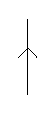
\includegraphics[scale=0.75]{graphics/particleline}
            \caption{Particle line}
        } \qquad
        \parbox{0.35\textwidth}{
            \centering
            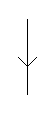
\includegraphics[scale=0.75]{graphics/holeline}
            \caption{Hole line}
        }
    \end{figure}

    \begin{itemize}
        \item A line represents a contraction between second quantized operators of the 
type $ \contraction{}{a}{{}^{\dagger}_i}{a}
    a^\dagger_i a_j=\delta_{ij}$ and  $\contraction{}{\an{a}}{}{\cre{b}}
\an{a}\cre{b}=\delta_{ab}$. 
        \item Hole (vacant) states are represented as downgoing lines 
        \item Particle (virtual) states are represented as upgoing lines
    \end{itemize}

\end{frame}
\begin{frame}{Diagram elements - Onebody Hamiltonian $\hat{F}_N =\sum_{pq} f_q^p \normord{a^\dagger_p a_q}$}
    \renewcommand{\figurename}{Level}
    \begin{figure}
    \centering
    \parbox{0.20\textwidth}{
            \centering
            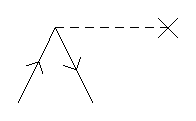
\includegraphics[scale=0.65]{graphics/f1}
            \caption{-1}
        }
        \parbox{0.20\textwidth}{
            \centering
            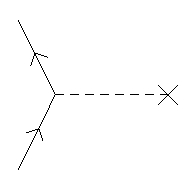
\includegraphics[scale=0.65]{graphics/f2}
            \caption{0}
        }
        \parbox{0.20\textwidth}{
            \centering
            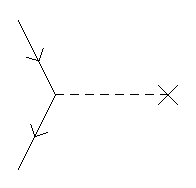
\includegraphics[scale=0.65]{graphics/f3}
            \caption{0}
        }
        \parbox{0.20\textwidth}{
            \centering
            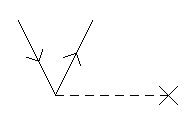
\includegraphics[scale=0.65]{graphics/f4}
            \caption{+1}
        }
    \end{figure}

    \begin{itemize}
        \item Horisontal dashed line segment with one vertex. Assume time axis pointing upward, with 
the state $\langle p|$ being above the vertex and the state $|q\rangle$ being below. 
        \item Excitation level identify the number of particle/hole pairs created by the operator.
    \end{itemize}
\end{frame}


\begin{frame}{Diagram elements - Twobody Hamiltonian $\hat{V}_N=\frac{1}{4} \sum_{pqrs} \bra{pq}\hat{v}\ket{rs} \normord{a^\dagger_p a^\dagger_q a_s  a_r}$}
    \renewcommand{\figurename}{Level}

    \begin{figure}
    \centering
    \parbox{0.30\textwidth}{
            \centering
            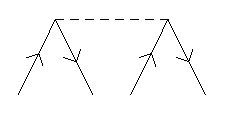
\includegraphics[scale=0.45]{graphics/v1}
            \caption{-2}
        }\quad
        \parbox{0.30\textwidth}{
            \centering
            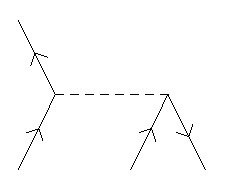
\includegraphics[scale=0.45]{graphics/v2}
            \caption{-1}
        }\quad
        \parbox{0.30\textwidth}{
            \centering
            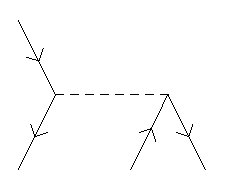
\includegraphics[scale=0.45]{graphics/v3}
            \caption{-1}
        }
    \end{figure}

    \begin{figure}
    \centering
    \parbox{0.30\textwidth}{
            \centering
            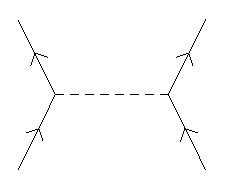
\includegraphics[scale=0.45]{graphics/v4}
            \caption{0}
        }\quad
        \parbox{0.30\textwidth}{
            \centering
            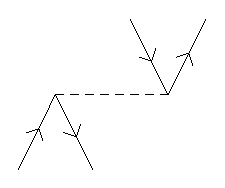
\includegraphics[scale=0.45]{graphics/v5}
            \caption{0}
        }\quad
        \parbox{0.30\textwidth}{
            \centering
            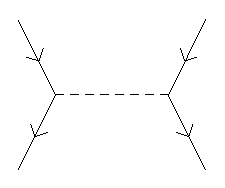
\includegraphics[scale=0.45]{graphics/v6}
            \caption{0}
        }
    \end{figure}

    \begin{figure}
    \centering
    \parbox{0.30\textwidth}{
            \centering
            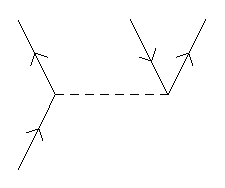
\includegraphics[scale=0.45]{graphics/v7}
            \caption{+1}
        }\quad
        \parbox{0.30\textwidth}{
            \centering
            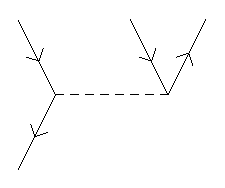
\includegraphics[scale=0.45]{graphics/v8}
            \caption{+1}
        }\quad
        \parbox{0.30\textwidth}{
            \centering
            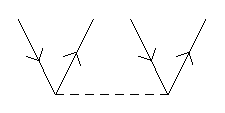
\includegraphics[scale=0.45]{graphics/v9}
            \caption{+2}
        }
    \end{figure}

\end{frame}

\begin{frame}{Diagram rules for operators}
    \begin{itemize}
        \item Label all lines.
        \item Sum over all indices. 
        \item For two-body operators draw dotted lines for the operator from endpoint to endpoint. 
Keep only topologically distinct diagrams and draw incoming and outgoing lines at every endpoint.
\item Mark the lines as either holes or particles. 
        \item Extract matrix elements from diagrams as follows: $f_{\mathrm{in}}^{\mathrm{out}}$ or 
$\langle \mathrm{out}|f|\mathrm{in}\rangle$, 
            $\bra{\mathrm{leftout, rightout}}\hat{v}\ket{\mathrm{leftin, rightin}}$)
\item For the two-body operators, crossing lines (below or above the interaction line) 
give rise to a minus sign.
\item For hole states, a hole line which goes through the whole diagram, add a minus sign.  
    \end{itemize}
\end{frame}





\frame
{
  \frametitle{Summary Particle-hole formalism}
\begin{small}
{\scriptsize
We defined the normal-ordered Hamiltonian wrt to the new vacuum as:
    \begin{block}{Twobody Hamiltonian}
    \begin{align*}
        \hat{H}_N &= 
            \frac{1}{4} \sum_{pqrs} \bra{pq}\hat{v}\ket{rs} \normord{a^\dagger_p a^\dagger_q a_s  a_r} 
            + \sum_{pq} f_q^p \normord{a^\dagger_p a_q} \\
        &= \hat{V}_N + \hat{F}_N
    \end{align*}
    where
    \begin{subequations}
    \begin{align*}
        \hat{F}_N &= \sum_{pq} f_q^p \normord{a^\dagger_p a_q} \\
        \hat{V}_N &= \frac{1}{4} \sum_{pqrs} \bra{pq}\hat{v}\ket{rs} \normord{a^\dagger_p a^\dagger_q a_s  a_r} \\
    \end{align*}
    \end{subequations}
How do we translate this to the standard particle-hole operators?
    \end{block}
}
\end{small}
}



\frame
{
  \frametitle{Summary: Particle-hole formalism}
\begin{small}
{\scriptsize
We can define
\[
	b_\alpha^\dagger = \Bigg\{ \begin{array}{ll}
		a_\alpha^\dagger & \alpha > F \\
		\\
		a_\alpha & \alpha \leq F
	\end{array} \qquad 
	b_\alpha = \Bigg\{ \begin{array}{ll}
		a_\alpha & \alpha > F \\
		\\
		 a_\alpha^\dagger & \alpha \leq F
	\end{array} 
\]
}
\end{small}
}


\frame
{
  \frametitle{Summary: Particle-hole formalism}
\begin{small}
{\scriptsize
The compact notation is 
\[
        \hat{H}_0 = \sum_{pq} \element{p}{h_0}{q} \normord{a^\dagger_p a_q} +\sum_{i} \element{i}{h_0}{i}.
\]
Spelling it out we can write $H_0$ as 
\begin{eqnarray}
	\hat{H}_0 &=& \sum_{ab} \element{a}{h_0}{b}  b_a^\dagger b_b +
		\sum_{ai} \left[
		\element{a}{h_0}{i} b_a^\dagger b_i^\dagger + 
		\element{i}{h_0}{a} b_i  b_a \right] \nonumber \\
	&+& \sum_{i} \element{i}{h_0}{i} - 
		\sum_{ij} \element{j}{h_0}{i}
		b_i^\dagger b_j \nonumber
\end{eqnarray}
}
\end{small}
}

\begin{frame}{This translates into the following diagram elements}
    \renewcommand{\figurename}{Level}
    \begin{figure}
    \centering
    \parbox{0.20\textwidth}{
            \centering
            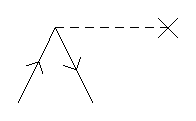
\includegraphics[scale=0.65]{graphics/f1}
            \caption{-1}
        }
        \parbox{0.20\textwidth}{
            \centering
            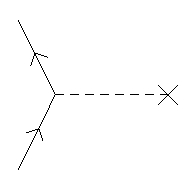
\includegraphics[scale=0.65]{graphics/f2}
            \caption{0}
        }
        \parbox{0.20\textwidth}{
            \centering
            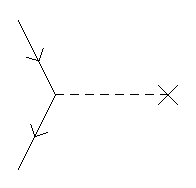
\includegraphics[scale=0.65]{graphics/f3}
            \caption{0}
        }
        \parbox{0.20\textwidth}{
            \centering
            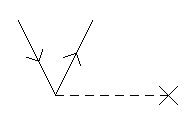
\includegraphics[scale=0.65]{graphics/f4}
            \caption{+1}
        }
    \end{figure}

    \begin{itemize}
        \item Horisontal dashed line segment with one vertex. Assume time axis pointing upward, with 
the state $\langle p|$ being above the vertex and the state $|q\rangle$ being below. 
        \item Excitation level identify the number of particle/hole pairs created by the operator.
    \end{itemize}
\end{frame}



\frame
{
  \frametitle{Summary: Particle-hole formalism}
\begin{small}
{\scriptsize
Similarly, the compact notation for the  two-body operator
    A twobody part
    \begin{equation*}
            \hat{V}_N \Leftarrow \frac{1}{4} \sum_{pqrs} \element{pq}{\hat{v}}{rs} 
                \normord{a^\dagger_p a^\dagger_q a_s  a_r}
    \end{equation*}
    A onebody part
    \begin{equation*}
            \hat{F}_N \Leftarrow \sum_{pqi} \element{pi}{\hat{v}}{qi} \normord{a^\dagger_p a_q}
    \end{equation*}
    and a scalar part
    \begin{equation*}
                E_0 \Leftarrow \frac{1}{2} \sum_{ij} \element{ij}{\hat{v}}{ij}
    \end{equation*}
has its root in the particle-hole operators as:
}
\end{small}
}



\frame
{
  \frametitle{Summary: Particle-hole formalism}
\begin{small}
{\scriptsize
\[
	\hat{H}_I = \hat{H}_I^{(a)} + \hat{H}_I^{(b)} + \hat{H}_I^{(c)} + \hat{H}_I^{(d)} + \hat{H}_I^{(e)}
\]
Using anti-symmetrized  matrix elements, 
the term  $\hat{H}_I^{(a)}$ is  
\[
	\hat{H}_I^{(a)} = \frac{1}{4}
	\sum_{abcd} \element{ab}{V}{cd} 
		b_a^\dagger b_b^\dagger b_d b_c 
\]
}
\end{small}
}


\frame
{
  \frametitle{Particle-hole formalism}
\begin{small}
{\scriptsize
The next term $\hat{H}_I^{(b)}$  reads
\[
	 \hat{H}_I^{(b)} = \frac{1}{2} \sum_{abci}\left(\element{ab}{V}{ci}b_a^\dagger b_b^\dagger b_i^\dagger b_c +\element{ai}{V}{cb}
		b_a^\dagger b_i b_b b_c\right)
\]
This term conserves the number of quasiparticles but creates or removes a 
three-particle-one-hole  state. 
For $\hat{H}_I^{(c)}$  we have
\begin{eqnarray}
	\hat{H}_I^{(c)}& =& \frac{1}{4}
		\sum_{abij}\left(\element{ab}{V}{ij}b_a^\dagger b_b^\dagger b_j^\dagger b_i^\dagger +
		\element{ij}{V}{ab}b_a  b_b b_j b_i \right)+  \nonumber \\
	&&	\sum_{abij}\element{ai}{V}{bj}b_a^\dagger b_j^\dagger b_b b_i + 
		\sum_{abi}\element{ai}{V}{bi}b_a^\dagger b_b. \nonumber
\end{eqnarray}
}
\end{small}
}


\frame
{
  \frametitle{Particle-hole formalism}
\begin{small}
{\scriptsize
The first line stands for the creation of a two-particle-two-hole state, while the second line represents
the creation to two one-particle-one-hole pairs
while the last term represents a contribution to the particle single-particle energy
from the hole states, that is an interaction between the particle states and the hole states
within the new vacuum  state.
The fourth term reads
\begin{eqnarray}
	 \hat{H}_I^{(d)}& = &\frac{1}{2} 
	 	\sum_{aijk}\left(\element{ai}{V}{jk}b_a^\dagger b_k^\dagger b_j^\dagger b_i+
\element{ji}{V}{ak}b_k^\dagger b_j b_i b_a\right)+\nonumber \\
&&\sum_{aij}\left(\element{ai}{V}{ji}b_a^\dagger b_j^\dagger+\element{ji}{V}{ai}b_j b_a \right). \nonumber
\end{eqnarray}
}
\end{small}
}


\frame
{
  \frametitle{Particle-hole formalism}
\begin{small}
{\scriptsize
The terms in the first line  stand for the creation of a particle-hole state 
interacting with hole states, we will label this as a two-hole-one-particle contribution. 
The remaining terms are a particle-hole state interacting with the holes in the vacuum state. 
Finally we have 
\[
	\hat{H}_I^{(e)} = \frac{1}{4}
		 \sum_{ijkl}
		 \element{kl}{V}{ij}b_i^\dagger b_j^\dagger b_l b_k
	        -\sum_{ijk}\element{ij}{V}{kj}b_k^\dagger b_i
	        +\frac{1}{2}\sum_{ij}\element{ij}{V}{ij}
\]
The first terms represents the 
interaction between two holes while the second stands for the interaction between a hole and the remaining holes in the vacuum state.
It represents a contribution to single-hole energy  to first order.
The last term collects all contributions to the energy of the ground state of a closed-shell system arising
from hole-hole correlations.
}
\end{small}
}


\section[Week 40]{Week 40}
\frame
{
  \frametitle{Topics for Week 40}
  \begin{block}{Hartree-Fock theory}
\begin{itemize}
\item Monday:
\item Summary from last week
\item Derivation of Hartree-Fock equations
\item Koopman's theorem
\item Tuesday:
\item Thouless' theorem
\item Stability of Hartree-Fock theory
\end{itemize}

  \end{block}
} 



\frame[containsverbatim]
{
  \frametitle{Hartree-Fock: our first many-body approach}
\begin{small}
{\scriptsize
HF theory is an algorithm for a finding an approximative expression for the ground state of a given
Hamiltonian. The basic ingredients are
\begin{itemize}
\item Define a single-particle basis $\{\psi_{\alpha}\}$ so that
\[ \hat{h}^{\mathrm{HF}}\psi_{\alpha} = \varepsilon_{\alpha}\psi_{\alpha}\]
with \[\hat{h}^{\mathrm{HF}}=\hat{t}+\hat{u}_{\matrhm{ext}}+\hat{u}^{\mathrm{HF}}\]
\item where $\hat{u}^{\mathrm{HF}}$ is a single-particle potential to be determined by the HF algorithm.
\item The HF algorithm means to choose $\hat{u}^{\mathrm{HF}}$ in order to have 
\[ \langle \hat{H} \rangle = E^{\mathrm{HF}}= \langle \Phi_0 | \hat{H}|\Phi_0 \rangle\]
a local minimum with $\Phi_0$ being the SD ansatz for the ground state. 
\item The variational principle ensures that $E^{\mathrm{HF}} \ge \tilde{E}_0$, $\tilde{E}_0$ the exact ground state energy.
\end{itemize}

 }
 \end{small}
 }


\frame[containsverbatim]
{
  \frametitle{Hartree-Fock: }
\begin{small}
{\scriptsize
Let us now compute the  Hamiltonian matrix for a system consisting of a Slater determinant for the ground state 
$|\Phi_0 \rangle$ and two 1p1h SDs $|\Phi_i^a \rangle$ and $|\Phi_j^b \rangle$. This can obviously be generalized to many more 1p1h SDs.  Using diagrammatic as well as algebraic representations we obtain the following 
expectation values
\[ \langle \Phi_0 | \hat{H}|\Phi_0 \rangle = E_0, \]
\[ \langle \Phi_i^a | \hat{H}|\Phi_0 \rangle = \langle a | \hat{f} | i \rangle,\]
\[ \langle \Phi_j^b | \hat{H}|\Phi_0 \rangle = \langle b | \hat{f} | j \rangle,\]
\[\langle \Phi_i^a | \hat{H}|\Phi_j^b \rangle = \langle aj | \hat{v} | ib \rangle,\]
and the diagonal elements
\[ \langle \Phi_i^a | \hat{H}|\Phi_i^a \rangle = E_0+\varepsilon_{a}-\varepsilon_{i}+\langle ai | \hat{v} | ia \rangle,\]
and 
\[ \langle \Phi_j^b | \hat{H}|\Phi_j^b \rangle =E_0+\varepsilon_{b}-\varepsilon_{j}+\langle bj | \hat{v} | jb \rangle.\]
 }
 \end{small}
 }



\frame[containsverbatim]
{
  \frametitle{Hartree-Fock}
\begin{small}
{\scriptsize
We can then set up a Hamiltonian matrix to be diagonalized
\[
 \left( \begin{array}{ccc} 
               E_0  & \langle i | \hat{f} | a \rangle &  \langle j | \hat{f} | b\rangle\\
               \langle a | \hat{f} | i \rangle  &E_0+\varepsilon_{a}-\varepsilon_{i}+\langle ai | \hat{v} | ia \rangle  & \langle aj | \hat{v} | ib \rangle      \\
               \langle b | \hat{f} | j \rangle  & \langle bi | \hat{v} | ja \rangle &E_0+\varepsilon_{b}-\varepsilon_{j}+\langle bj | \hat{v} | jb \rangle         \\
             \end{array} \right) .
\]
The HF method corresponds to finding a similarity transformation where the non-diagonal matrix elements
\[\langle i | \hat{f} | a \rangle=0\].   We will link this expectation value with the HF method, meaning that
we want to find
\[\langle i | \hat{h}^{\mathrm{HF}}| a \rangle=0\]
 }
 \end{small}
 }

\frame[containsverbatim]
{
  \frametitle{Variational Calculus and Lagrangian Multiplier}
\begin{small}
{\scriptsize
The calculus of variations involves 
problems where the quantity to be minimized or maximized is an integral. 

In the general case we have an integral of the type
\[ E[\Phi]= \int_a^b f(\Phi(x),\frac{\partial \Phi}{\partial x},x)dx,\]
where $E$ is the quantity which is sought minimized or maximized.
The problem is that although $f$ is a function of the variables $\Phi$, $\partial \Phi/\partial x$ and $x$, the exact dependence of
$\Phi$ on $x$ is not known.  This means again that even though the integral has fixed limits $a$ and $b$, the path of integration is
not known. In our case the unknown quantities are the single-particle wave functions and we wish to choose an integration path which makes
the functional $E[\Phi]$ stationary. This means that we want to find minima, or maxima or saddle points. In physics we search normally for minima.
Our task is therefore to find the minimum of $E[\Phi]$ so that its variation $\delta E$ is zero  subject to specific
constraints. In our case the constraints appear as the integral which expresses the orthogonality of the  single-particle wave functions.
The constraints can be treated via the technique of Lagrangian multipliers
 }
 \end{small}
 }




\frame[containsverbatim]
{
  \frametitle{Reminder on Variational Calculus and Lagrangian Multipliers}
\begin{small}
{\scriptsize
Let us specialize to the expectation value of the energy for one particle in three-dimensions.
This expectation value reads
\[
  E=\int dxdydz \psi^*(x,y,z) \hat{H} \psi(x,y,z),
\]
with the constraint
\[
 \int dxdydz \psi^*(x,y,z) \psi(x,y,z)=1,
\]
and a Hamiltonian
\[
\hat{H}=-\frac{1}{2}\nabla^2+V(x,y,z).
\]
I will skip the variables $x,y,z$ below, and write for example $V(x,y,z)=V$.
 }
 \end{small}
 }


\frame[containsverbatim]
{
  \frametitle{Variational Calculus and Lagrangian Multiplier}
\begin{small}
{\scriptsize
The integral involving the kinetic energy can be written as, if we assume periodic boundary conditions or that the function $\psi$ vanishes
strongly for large values of $x,y,z$, 
 \[
  \int dxdydz \psi^* \left(-\frac{1}{2}\nabla^2\right) \psi dxdydz = \psi^*\nabla\psi|+\int dxdydz\frac{1}{2}\nabla\psi^*\nabla\psi.
\]
Inserting this expression into the expectation value for the energy and taking the variational minimum  we obtain
\[
\delta E = \delta \left\{\int dxdydz\left( \frac{1}{2}\nabla\psi^*\nabla\psi+V\psi^*\psi\right)\right\} = 0.
\]
 }
 \end{small}
 }

\frame[containsverbatim]
{
  \frametitle{Variational Calculus and Lagrangian Multiplier}
\begin{small}
{\scriptsize
The constraint appears in integral form as 
\[
 \int dxdydz \psi^* \psi=\mathrm{constant},
\]
and multiplying with a Lagrangian multiplier $\lambda$ and taking the variational minimum we obtain the final variational equation
\[
\delta \left\{\int dxdydz\left( \frac{1}{2}\nabla\psi^*\nabla\psi+V\psi^*\psi-\lambda\psi^*\psi\right)\right\} = 0.
\]
Introducing the function  $f$
\[
  f =  \frac{1}{2}\nabla\psi^*\nabla\psi+V\psi^*\psi-\lambda\psi^*\psi=
\frac{1}{2}(\psi^*_x\psi_x+\psi^*_y\psi_y+\psi^*_z\psi_z)+V\psi^*\psi-\lambda\psi^*\psi,
\]
where we have skipped the dependence on $x,y,z$ and introduced the shorthand $\psi_x$, $\psi_y$ and $\psi_z$  for the various derivatives.
 }
 \end{small}
 }


\frame[containsverbatim]
{
  \frametitle{Variational Calculus and Lagrangian Multiplier}
\begin{small}
{\scriptsize
For $\psi^*$ the Euler  equation results in
\[
\frac{\partial f}{\partial \psi^*}- \frac{\partial }{\partial x}\frac{\partial f}{\partial \psi^*_x}-\frac{\partial }{\partial y}\frac{\partial f}{\partial \psi^*_y}-\frac{\partial }{\partial z}\frac{\partial f}{\partial \psi^*_z}=0,
\] 
which yields 
\[
    -\frac{1}{2}(\psi_{xx}+\psi_{yy}+\psi_{zz})+V\psi=\lambda \psi.
\]
We can then identify the  Lagrangian multiplier as the energy of the system. Then the last equation is 
nothing but the standard 
Schr\"odinger equation and the variational  approach discussed here provides 
a powerful method for obtaining approximate solutions of the wave function.

 }
 \end{small}
 }


\frame[containsverbatim]
{
  \frametitle{Finding the Hartree-Fock functional $E[\Phi]$}
\begin{small}
{\scriptsize
We rewrite our Hamiltonian (we specialize to atomic physics, but the interactions can easily be changed with other one and two-body ones)
\[
  \hat{H} = -\sum_{i=1}^N \frac{1}{2} \nabla^2_i 
  - \sum_{i=1}^N \frac{Z}{r_i} + \sum_{i<j}^N \frac{1}{r_{ij}},
\]
as
\[
    \hat{H} = \hat{H_0} + \hat{H_I} 
    = \sum_{i=1}^N\hat{h_o}(x_i) + \sum_{i<j=1}^N\frac{1}{r_{ij}},
\]

\[
  \hat{h}_0(x_i) = - \frac{1}{2} \nabla^2_i - \frac{Z}{r_i}.
\]
 }
 \end{small}
 }


\frame[containsverbatim]
{
  \frametitle{Finding the Hartree-Fock functional $E[\Phi]$}
\begin{small}
{\scriptsize
Let us denote the ground state energy by $E_0$. According to the
variational principle we have
\begin{equation*}
  E_0 \le E[\Phi] = \int \Phi^*\hat{H}\Phi d\mathbf{\tau}
\end{equation*}
where $\Phi$ is a trial function which we assume to be normalized
\begin{equation*}
  \int \Phi^*\Phi d\mathbf{\tau} = 1,
\end{equation*}
where we have used the shorthand $d\mathbf{\tau}=dx_1dx_2\dots dx_N$.
 }
 \end{small}
 }


\frame[containsverbatim]
{
  \frametitle{Finding the Hartree-Fock functional $E[\Phi]$}
\begin{small}
{\scriptsize
In the Hartree-Fock method the trial function is the Slater
determinant which can be rewritten as 
\[
  \Psi(x_1,x_2,\dots,x_N,\alpha,\beta,\dots,\nu) = \frac{1}{\sqrt{N!}}\sum_{P} (-)^PP\psi_{\alpha}(x_1)
    \psi_{\beta}(x_2)\dots\psi_{\nu}(x_N)=\sqrt{N!}{\cal A}\Phi_H,
\]
where we have introduced the anti-symmetrization operator ${\cal A}$ defined by the 
summation over all possible permutations of two fermions.
It is defined as
\[
  {\cal A} = \frac{1}{N!}\sum_{P} (-)^PP,
\]
with the the Hartree-function given by the simple product of all possible single-particle function (in case of atomic systems: 
two electrons for helium, four electrons for beryllium and ten for
neon)
\[
  \Phi_H(x_1,x_2,\dots,x_N,\alpha,\beta,\dots,\nu) =
  \psi_{\alpha}(x_1)
    \psi_{\beta}(x_2)\dots\psi_{\nu}(x_N).
\]

 }
 \end{small}
 }


\frame[containsverbatim]
{
  \frametitle{Finding the Hartree-Fock functional $E[\Phi]$}
\begin{small}
{\scriptsize
Both $\hat{H_0}$ and $\hat{H_I}$ are invariant under 
permutations of fermions, and hence commute with ${\cal A}$
\[
  [H_0,{\cal A}] = [H_I,{\cal A}] = 0.
\]
Furthermore, ${\cal A}$ satisfies
\[
  {\cal A}^2 = {\cal A},
\]
since every permutation of the Slater
determinant reproduces it.
 }
 \end{small}
 }


\frame[containsverbatim]
{
  \frametitle{Variational Calculus and Lagrangian Multiplier, back to Hartree-Fock}
\begin{small}
{\scriptsize
Our functional is written (recall that we have specialized to the case of atoms) as 
\[
  E[\Phi] = \sum_{\mu=1}^N \int \psi_{\mu}^*(x_i)\hat{h}_0(x_i)\psi_{\mu}(x_i) dx_i 
  + \frac{1}{2}\sum_{\mu=1}^N\sum_{\nu=1}^N
   \left[ \int \psi_{\mu}^*(x_i)\psi_{\nu}^*(x_j)\frac{1} 
    {r_{ij}}\psi_{\mu}(x_i)\psi_{\nu}(x_j)
    dx_idx_j \right.
\]
\[ \left.
  - \int \psi_{\mu}^*(x_i)\psi_{\nu}^*(x_j)
  \frac{1}{r_{ij}}\psi_{\nu}(x_i)\psi_{\mu}(x_j)
  dx_idx_j\right]
\]
The more compact version is
\[
  E[\Phi] 
  = \sum_{\mu=1}^N \langle \mu | \hat{h}_0 | \mu\rangle+ \frac{1}{2}\sum_{\mu=1}^N\sum_{\nu=1}^N\left[\langle \mu\nu |\frac{1}{r_{ij}}|\mu\nu\rangle-\langle \mu\nu |\frac{1}{r_{ij}}|\nu\mu\rangle\right].
\]
 }
 \end{small}
 }



\frame[containsverbatim]
{
  \frametitle{Hartree-Fock: Variational Calculus and Lagrangian Multiplier}
\begin{small}
{\scriptsize
If we generalize the Euler-Lagrange equations to more variables 
and introduce $N^2$ Lagrange multipliers which we denote by 
$\epsilon_{\mu\nu}$, we can write the variational equation for the functional of $E$
\[
  \delta E - \sum_{{\mu}=1}^N\sum_{{\nu}=1}^N \epsilon_{\mu\nu} \delta
  \int \psi_{\mu}^* \psi_{\nu} = 0.
\]
For the orthogonal wave functions $\psi_{\mu}$ this reduces to
\[
  \delta E - \sum_{{\mu}=1}^N \epsilon_{\mu} \delta
  \int \psi_{\mu}^* \psi_{\mu} = 0.
\]
 }
 \end{small}
 }


\frame[containsverbatim]
{
  \frametitle{Hartree-Fock: Variational Calculus and Lagrangian Multiplier}
\begin{small}
{\scriptsize
Variation with respect to the single-particle wave functions $\psi_{\mu}$ yields then

\begin{equation*}
\begin{split}
  \sum_{\mu=1}^N \int \delta\psi_{\mu}^*\hat{h_0}(x_i)\psi_{\mu}
  dx_i  
  + \frac{1}{2}\sum_{{\mu}=1}^N\sum_{{\nu}=1}^N \left[ \int
  \delta\psi_{\mu}^*\psi_{\nu}^*\frac{1} 
  {r_{ij}}\psi_{\mu}\psi_{\nu} dx_idx_j- \int
  \delta\psi_{\mu}^*\psi_{\nu}^*\frac{1}{r_{ij}}\psi_{\nu}\psi_{\mu}
  dx_idx_j \right] & \\
  + \sum_{\mu=1}^N \int \psi_{\mu}^*\hat{h_0}(x_i)\delta\psi_{\mu}
  dx_i 
  + \frac{1}{2}\sum_{{\mu}=1}^N\sum_{{\nu}=1}^N \left[ \int
  \psi_{\mu}^*\psi_{\nu}^*\frac{1} 
  {r_{ij}}\delta\psi_{\mu}\psi_{\nu} dx_idx_j- \int
  \psi_{\mu}^*\psi_{\nu}^*\frac{1}{r_{ij}}\psi_{\nu}\delta\psi_{\mu}
  dx_idx_j \right] & \\
  -  \sum_{{\mu}=1}^N E_{\mu} \int \delta\psi_{\mu}^*
  \psi_{\mu}dx_i
  -  \sum_{{\mu}=1}^N E_{\mu} \int \psi_{\mu}^*
  \delta\psi_{\mu}dx_i & = 0.
\end{split}
\end{equation*}

 }
 \end{small}
 }


\frame[containsverbatim]
{
  \frametitle{Hartree-Fock: Variational Calculus and Lagrangian Multiplier}
\begin{small}
{\scriptsize
Although the variations $\delta\psi$ and $\delta\psi^*$ are not
independent, they may in fact be treated as such, so that the 
terms dependent on either $\delta\psi$ and $\delta\psi^*$ individually 
may be set equal to zero. To see this, simply 
replace the arbitrary variation $\delta\psi$ by $i\delta\psi$, so that
$\delta\psi^*$ is replaced by $-i\delta\psi^*$, and combine the two
equations. We thus arrive at the Hartree-Fock equations
\[
  \begin{split}
    \left[ -\frac{1}{2}\nabla_i^2-\frac{Z}{r_i} + \sum_{{\nu}=1}^N
      \int \psi_{\nu}^*(x_j)\frac{1}{r_{ij}}
      \psi_{\nu}(x_j)dx_j \right]
    \psi_{\mu}(x_i)  & \\
    - \left[ \sum_{{\nu}=1}^N \int
      \psi_{\nu}^*(x_j) 
      \frac{1}{r_{ij}}\psi_{\mu}(x_j) dx_j
      \right] \psi_{\nu}(x_i)  & 
  = \epsilon_{\mu} \psi_{\mu}(x_i).
  \end{split}
\]
Notice that the integration $\int dx_j$ implies an
integration over the spatial coordinates $\mathbf{r_j}$ and a summation
over the spin-coordinate of fermion $j$.
 }
 \end{small}
 }


\frame[containsverbatim]
{
  \frametitle{Hartree-Fock: Variational Calculus and Lagrangian Multiplier}
\begin{small}
{\scriptsize
The two first terms are the one-body kinetic energy and the
electron-nucleus potential. The third or
\emph{direct} term is the averaged electronic repulsion of the other
electrons. This term is identical to the Coulomb integral introduced in
the simple perturbative approach to the helium atom. As written, the
term includes the 'self-interaction' of 
electrons when $i=j$. The self-interaction is cancelled in the fourth
term, or the \emph{exchange} term. The exchange term results from our
inclusion of the Pauli principle and the assumed determinantal form of
the wave-function. The effect of exchange is for electrons of
like-spin to avoid each other.
 }
 \end{small}
 }


\frame[containsverbatim]
{
  \frametitle{Hartree-Fock: Variational Calculus and Lagrangian Multiplier}
\begin{small}
{\scriptsize
  A theoretically convenient form of the
Hartree-Fock equation is to regard the direct and exchange operator
defined through 
\begin{equation*}
  V_{\mu}^{d}(x_i) = \int \psi_{\mu}^*(x_j) 
  \frac{1}{r_{ij}}\psi_{\mu}(x_j) dx_j
\end{equation*}
and
\begin{equation*}
  V_{\mu}^{ex}(x_i) g(x_i) 
  = \left(\int \psi_{\mu}^*(x_j) 
  \frac{1}{r_{ij}}g(x_j) dx_j
  \right)\psi_{\mu}(x_i),
\end{equation*}
respectively. 
 }
 \end{small}
 }


\frame[containsverbatim]
{
  \frametitle{Hartree-Fock: Variational Calculus and Lagrangian Multiplier}
\begin{small}
{\scriptsize
The function $g(x_i)$ is an arbitrary function,
and by the substitution $g(x_i) = \psi_{\nu}(x_i)$
we get
\begin{equation*}
  V_{\mu}^{ex}(x_i) \psi_{\nu}(x_i) 
  = \left(\int \psi_{\mu}^*(x_j) 
  \frac{1}{r_{ij}}\psi_{\nu}(x_j)
  dx_j\right)\psi_{\mu}(x_i).
\end{equation*}
 }
 \end{small}
 }


\frame[containsverbatim]
{
  \frametitle{Hartree-Fock: Variational Calculus and Lagrangian Multiplier}
\begin{small}
{\scriptsize
We may then rewrite the Hartree-Fock equations as
\[
  \hat{h}^{HF}(x_i) \psi_{\nu}(x_i) = \epsilon_{\nu}\psi_{\nu}(x_i),
\]
with
\[
  \hat{h}^{HF}(x_i)= \hat{h}_0(x_i) + \sum_{\mu=1}^NV_{\mu}^{d}(x_i) -
  \sum_{\mu=1}^NV_{\mu}^{ex}(x_i),
\]
and where $\hat{h}_0(i)$ is the one-body part. The latter is normally chosen as a part which yields solutions in closed form. The harmonic oscilltor is a classical problem thereof.
We normally rewrite the last equation as
\[
  \hat{h}^{HF}(x_i)= \hat{h}_0(x_i) + \hat{u}^{HF}(x_i). 
\]
 }
 \end{small}
 }


\frame[containsverbatim]
{
  \frametitle{Rewriting the energy functional}
\begin{small}
{\scriptsize
The last equation 
\[
  \hat{h}^{HF}(x_i)= \hat{h}_0(x_i) + \hat{u}^{HF}(x_i), 
\]
allows us to rewrite the ground state energy (adding and subtracting $\hat{u}^{HF}(x_i)$ 
\[
  E_0^{HF} =\langle \Phi_0 | \hat{H} | \Phi_0\rangle = 
\sum_{i\le F}^N \langle i | \hat{h}_0 +\hat{u}^{HF}| j\rangle+ \frac{1}{2}\sum_{i\le F}^N\sum_{j \le F}^N\left[\langle ij |\hat{v}|ij \rangle-\langle ij|\hat{v}|ji\rangle\right]-\sum_{i\le F}^N \langle i |\hat{u}^{HF}| i\rangle,
\]
as
\[
  E_0^{HF}
  = \sum_{i\le F}^N \varepsilon_i + \frac{1}{2}\sum_{i\le F}^N\sum_{j \le F}^N\left[\langle ij |\hat{v}|ij \rangle-\langle ij|\hat{v}|ji\rangle\right]-\sum_{i\le F}^N \langle i |\hat{u}^{HF}| i\rangle,
\]
which is nothing but
\[
  E_0^{HF}
  = \sum_{i\le F}^N \varepsilon_i - \frac{1}{2}\sum_{i\le F}^N\sum_{j \le F}^N\left[\langle ij |\hat{v}|ij \rangle-\langle ij|\hat{v}|ji\rangle\right].
\]
This form will be used in our discussion of Koopman's theorem.
 }
 \end{small}
 }


\frame[containsverbatim]
{
  \frametitle{Hartree-Fock by varying the coefficients of a wave function expansion}
\begin{small}
{\scriptsize

Another possibility is to expand the single-particle functions in a known basis  and vary the coefficients, 
that is, the new single-particle wave function is written as a linear expansion
in terms of a fixed chosen orthogonal basis (for example harmonic oscillator, Laguerre polynomials etc)
\be
\psi_a  = \sum_{\lambda} C_{a\lambda}\psi_{\lambda}.
\label{eq:newbasis}
\ee
In this case we vary the coefficients $C_{a\lambda}$. If the basis has infinitely many solutions, we need
to truncate the above sum.  In all our equations we assume a truncation has been made.

The single-particle wave functions $\psi_{\lambda}({\bf r})$, defined by the quantum numbers $\lambda$ and ${\bf r}$
are defined as the overlap 
\[
   \psi_{\lambda}({\bf r})  = \langle {\bf r} | \lambda \rangle .
\]
 }
 \end{small}
 }

\frame[containsverbatim]
{
  \frametitle{Hartree-Fock by varying the coefficients of a wave function expansion}
\begin{small}
{\scriptsize
We will omit the radial dependence of the wave functions and 
introduce first the following shorthands for the Hartree and Fock integrals
\[
\langle \mu\nu|V|\mu\nu\rangle =  \int \psi_{\mu}^*(\mathbf{r}_i)\psi_{\nu}^*(\mathbf{r}_j)V(r_{ij})\psi_{\mu}(\mathbf{r}_i)\psi_{\nu}(\mathbf{r}_j)
    d\mathbf{r}_i\mathbf{r}_j,
\]
and 
\[
\langle \mu\nu|V|\nu\mu\rangle = \int \psi_{\mu}^*(\mathbf{r}_i)\psi_{\nu}^*(\mathbf{r}_j)
  V(r_{ij})\psi_{\nu}(\mathbf{r}_i)\psi_{\mu}(\mathbf{r}_i)
  d\mathbf{r}_i\mathbf{r}_j.  
\]
 }
 \end{small}
 }

\frame[containsverbatim]
{
  \frametitle{Hartree-Fock by varying the coefficients of a wave function expansion}
\begin{small}
{\scriptsize
Since the interaction is invariant under the interchange of two particles it means for example that we have
\[
\langle \mu\nu|V|\mu\nu\rangle =  \langle \nu\mu|V|\nu\mu\rangle,  
\]
or in the more general case
\[
\langle \mu\nu|V|\sigma\tau\rangle =  \langle \nu\mu|V|\tau\sigma\rangle.  
\]
 }
 \end{small}
 }

\frame[containsverbatim]
{
  \frametitle{Hartree-Fock by varying the coefficients of a wave function expansion}
\begin{small}
{\scriptsize
The direct and exchange matrix elements can be  brought together if we define the antisymmetrized matrix element
\[
\langle \mu\nu|V|\mu\nu\rangle_{AS}= \langle \mu\nu|V|\mu\nu\rangle-\langle \mu\nu|V|\nu\mu\rangle,
\]
or for a general matrix element  
\[
\langle \mu\nu|V|\sigma\tau\rangle_{AS}= \langle \mu\nu|V|\sigma\tau\rangle-\langle \mu\nu|V|\tau\sigma\rangle.
\]
It has the symmetry property
\[
\langle \mu\nu|V|\sigma\tau\rangle_{AS}= -\langle \mu\nu|V|\tau\sigma\rangle_{AS}=-\langle \nu\mu|V|\sigma\tau\rangle_{AS}.
\]
The antisymmetric matrix element is also hermitian, implying 
\[
\langle \mu\nu|V|\sigma\tau\rangle_{AS}= \langle \sigma\tau|V|\mu\nu\rangle_{AS}.
\]
 }
 \end{small}
 }

\frame[containsverbatim]
{
  \frametitle{Hartree-Fock by varying the coefficients of a wave function expansion}
\begin{small}
{\scriptsize
With these notations we rewrite the Hartree-Fock functional as
\begin{equation}
  \int \Phi^*\hat{H_1}\Phi d\mathbf{\tau} 
  = \frac{1}{2}\sum_{\mu=1}^A\sum_{\nu=1}^A \langle \mu\nu|V|\mu\nu\rangle_{AS}.
\label{H2Expectation2}
\end{equation}


Combining Eqs.~(\ref{H1Expectation1}) and
(\ref{H2Expectation2}) we obtain the energy functional 
\begin{equation}
  E[\Phi] 
  = \sum_{\mu=1}^N \langle \mu | h | \mu \rangle +
  \frac{1}{2}\sum_{{\mu}=1}^N\sum_{{\nu}=1}^N \langle \mu\nu|V|\mu\nu\rangle_{AS}.
\label{FunctionalEPhi}
\end{equation}
 }
 \end{small}
 }

\frame[containsverbatim]
{
  \frametitle{Hartree-Fock by varying the coefficients of a wave function expansion}
\begin{small}
{\scriptsize
If we vary the above energy functional with respect to the basis functions $|\mu \rangle$, this corresponds to 
what was done in the previous case. We are however interested in defining a new basis defined in terms of
a chosen basis as defined in Eq.~(\ref{eq:newbasis}). We can then rewrite the energy functional as
\begin{equation}
  E[\Psi] 
  = \sum_{a=1}^N \langle a | h | a \rangle +
  \frac{1}{2}\sum_{ab=1}^N\langle ab|V|ab\rangle_{AS},
\label{FunctionalEPhi2}
\end{equation}
where $\Psi$ is the new Slater determinant defined by the new basis of Eq.~(\ref{eq:newbasis}). 

 }
 \end{small}
 }

\frame[containsverbatim]
{
  \frametitle{Hartree-Fock by varying the coefficients of a wave function expansion}
\begin{small}
{\scriptsize
Using Eq.~(\ref{eq:newbasis}) we can rewrite Eq.~(\ref{FunctionalEPhi2}) as 
\begin{equation}
  E[\Psi] 
  = \sum_{a=1}^N \sum_{\alpha\beta} C^*_{a\alpha}C_{a\beta}\langle \alpha | h | \beta \rangle +
  \frac{1}{2}\sum_{ab=1}^N\sum_{{\alpha\beta\gamma\delta}} C^*_{a\alpha}C^*_{b\beta}C_{a\gamma}C_{b\delta}\langle \alpha\beta|V|\gamma\delta\rangle_{AS}.
\label{FunctionalEPhi3}
\end{equation}
 }
 \end{small}
 }

\frame[containsverbatim]
{
  \frametitle{Hartree-Fock by varying the coefficients of a wave function expansion}
\begin{small}
{\scriptsize
We wish now to minimize the above functional. We introduce again a set of Lagrange multipliers, noting that
since $\langle a | b \rangle = \delta_{a,b}$ and $\langle \alpha | \beta \rangle = \delta_{\alpha,\beta}$, 
the coefficients $C_{a\gamma}$ obey the relation
\[
 \langle a | b \rangle=\delta_{a,b}=\sum_{\alpha\beta} C^*_{a\alpha}C_{a\beta}\langle \alpha | \beta \rangle=
\sum_{\alpha} C^*_{a\alpha}C_{a\alpha},
\]
which allows us to define a functional to be minimized that reads
\begin{equation}
  E[\Psi] - \sum_{a=1}^N\epsilon_a\sum_{\alpha} C^*_{a\alpha}C_{a\alpha}.
\end{equation}
 }
 \end{small}
 }

\frame[containsverbatim]
{
  \frametitle{Hartree-Fock by varying the coefficients of a wave function expansion}
\begin{small}
{\scriptsize
Minimizing with respect to $C^*_{k\alpha}$, remembering that $C^*_{k\alpha}$ and $C_{k\alpha}$
are independent, we obtain
\be
\frac{d}{dC^*_{k\alpha}}\left[  E[\Psi] - \sum_{a}\epsilon_a\sum_{\alpha} C^*_{a\alpha}C_{a\alpha}\right]=0,
\ee
which yields for every single-particle state $k$ the following Hartree-Fock equations
\be
\sum_{\gamma} C_{k\gamma}\langle \alpha | h | \gamma \rangle+
\sum_{a=1}^N\sum_{\beta\gamma\delta} C^*_{a\beta}C_{a\delta}C_{k\gamma}\langle \alpha\beta|V|\gamma\delta\rangle_{AS}=\epsilon_kC_{k\alpha}.
\ee
 }
 \end{small}
 }

\frame[containsverbatim]
{
  \frametitle{Hartree-Fock by varying the coefficients of a wave function expansion}
\begin{small}
{\scriptsize
We can rewrite this equation as 
\be
\sum_{\gamma} \left\{\langle \alpha | h | \gamma \rangle+
\sum_{a}^N\sum_{\beta\delta} C^*_{a\beta}C_{a\delta}\langle \alpha\beta|V|\gamma\delta\rangle_{AS}\right\}C_{k\gamma}=\epsilon_kC_{k\alpha}.
\ee
Note that the sums over greek indices run over the number of basis set functions (in principle an infinite number).
 }
 \end{small}
 }

\frame[containsverbatim]
{
  \frametitle{Hartree-Fock by varying the coefficients of a wave function expansion}
\begin{small}
{\scriptsize
Defining 
\[
h_{\alpha\gamma}^{HF}=\langle \alpha | h | \gamma \rangle+
\sum_{a=1}^N\sum_{\beta\delta} C^*_{a\beta}C_{a\delta}\langle \alpha\beta|V|\gamma\delta\rangle_{AS},
\]
we can rewrite the new equations as 
\be
\sum_{\gamma}h_{\alpha\gamma}^{HF}C_{k\gamma}=\epsilon_kC_{k\alpha}.
\label{eq:newhf}
\ee
Note again that the sums over greek indices run over the number of basis set functions (in principle an infinite number).
 }
 \end{small}
 }




{
  \frametitle{Hartree-Fock formalism in second quantization, Thouless' theorem}
\begin{small}
{\scriptsize
We wish now to derive the Hartree-Fock equations using our second-quantized formalism and study the stability of the equations. 
Our SD ansatz for the ground state of the system is approximated as
\[   |\Phi_0\rangle = |c\rangle = \cre{i} \cre{j}\dots\cre{l}|0\rangle.\]
We wish to determine $\hat{u}^{HF}$ so that 
$E_0^{HF}= \langle c|\hat{H}| c\rangle$ becomes a local minimum. 

An arbitrary Slater determinant $\ket{c'}$ which is not orthogonal to a determinant
$\ket{c}={\displaystyle\prod_{i=1}^{n}}
a_{i}^{\dagger}\ket{0}$, can be written as
\[
\ket{c'}=exp\left\{\sum_{a>F}^{\infty}
\sum_{i\le F}C_{ai}a_{a}^{\dagger}
a_{i}\right\}\ket{c}
\]
 }
 \end{small}
 }

\frame[containsverbatim]
{
  \frametitle{Thouless' theorem}
\begin{small}
{\scriptsize
An arbitrary Slater determinant $\ket{c'}$ which is not orthogonal to a determinant
$\ket{c}={\displaystyle\prod_{i=1}^{n}}
a_{\alpha_{i}}^{\dagger}\ket{0}$, can be written as
\[
\ket{c'}=exp\left\{\sum_{a>F}\sum_{i\le F}C_{ai}a_{a}^{\dagger}
a_{i}\right\}\ket{c}
\]
Proof: see blackboard.
 }
 \end{small}
 }

\frame[containsverbatim]
{
  \frametitle{Stability of the Hartree-Fock equations}
\begin{small}
{\scriptsize
The variational condition for deriving the Hartree-Fock equations guarantees only that the expectation value
$\langle c | \hat{H} | c \rangle$ has an extreme value, not necessarily a minimum. To figure out whether the extreme value we have found  is a minimum, we can use second quantization to analyze our results and find a criterion 
for the above expectation value to a local minimum. We will use Thouless' theorem and show that
\[
\frac{\langle c' |\hat{H} | c'\rangle}{\langle c' |c'\rangle} \ge \langle c |\hat{H} | c\rangle= E_0,
\]
with 
\[
|c'\rangle = |c\rangle + |\delta c\rangle.
\]
Using Thouless' theorem we can write out $|c'\rangle$ as
\[
\ket{c'}=exp\left\{\sum_{a>F}
\sum_{i\le F}\delta C_{ai}a_{a}^{\dagger}
a_{i}\right\}\ket{c}=
\]
\[
\left\{1+\sum_{a>F}\sum_{i\le F}\delta C_{ai}a_{a}^{\dagger}
a_{i}+\frac{1}{2!}\sum_{ab>F}
\sum_{ij\le F}\delta C_{ai}\delta C_{bj}a_{a}^{\dagger}a_{i}a_{b}^{\dagger}a_{j}+\dots\right\}
\]
where the amplitudes $\delta C$ are small.
 }
 \end{small}
 }

\frame[containsverbatim]
{
  \frametitle{Stability of the Hartree-Fock equations}
\begin{small}
{\scriptsize
The norm of $|c'\rangle$ is given by (using the intermediate normalization condition $\langle c' |c\rangle=1$) 
\[
\langle c' | c'\rangle = 1+\sum_{a>F}
\sum_{i\le F}|\delta C_{ai}|^2+O(\delta C_{ai}^3).
\]
The expectation value for the energy is now given by (using the Hartree-Fock condition)
\[
\langle c' |\hat{H} | c'\rangle=\langle c |\hat{H} | c\rangle +
\sum_{ab>F}
\sum_{ij\le F}\delta C_{ai}^*\delta C_{bj}\langle c |a_{i}^{\dagger}a_{a}\hat{H}a_{b}^{\dagger}a_{j}|c\rangle+
\]
\[
\frac{1}{2!}\sum_{ab>F}
\sum_{ij\le F}\delta C_{ai}\delta C_{bj}\langle c |\hat{H}a_{a}^{\dagger}a_{i}a_{b}^{\dagger}a_{j}|c\rangle+\frac{1}{2!}\sum_{ab>F}
\sum_{ij\le F}\delta C_{ai}^*\delta C_{bj}^*\langle c|a_{j}^{\dagger}a_{b}a_{i}^{\dagger}a_{a}\hat{H}|c\rangle
+\dots
\] 
We will skip higher-order terms later.
}
 \end{small}
 }

\frame[containsverbatim]
{
  \frametitle{Stability of the Hartree-Fock equations}
\begin{small}
{\scriptsize
We have already calculated the second term on the rhs of the previous equation
\[
\bra{c} \left(\normord{a^\dagger_i a_a} \op{H} \normord{a^\dagger_b a_j} \right) \ket{c} =
\]
\[
\sum_{pq} \sum_{ijab}\delta C_{ai}^*\delta C_{bj} \bra{p}\hat{h}_0\ket{q} 
            \bra{c} \left(\normord{a^\dagger_i a_a}\normord{a^\dagger_pa_q} 
             \normord{a^\dagger_b a_j} \right)\ket{c}+ 
\]
\[
\frac{1}{4} \sum_{pqrs} \sum_{ijab}\delta C_{ai}^*\delta C_{bj} \bra{pq}\hat{v}\ket{rs} 
            \bra{c} \left(\normord{a^\dagger_i a_a}\normord{a^\dagger_p a^\dagger_q a_s  a_r} \normord{a^\dagger_b a_j} \right)\ket{c},
\]
resulting in
\[
E_0\sum_{ai}|\delta C_{ai}|^2+\sum_{ai}|\delta C_{ai}|^2(\varepsilon_a-\varepsilon_i)-\sum_{ijab} \bra{aj}\hat{v}\ket{bi}\delta C_{ai}^*\delta C_{bj}.
\]
 }
 \end{small}
 }



\frame[containsverbatim]
{
  \frametitle{Stability of the Hartree-Fock equations}
\begin{small}
{\scriptsize
The third term in the rhs of the last equation can then be written out (where is the reference energy and why do we only consider the two-particle interaction $\hat{V}_N$?)
    \begin{align*}
        & \frac{1}{2!}\bra{c}  \left( \op{V}_N \normord{a^\dagger_a a_i} \normord{a^\dagger_b a_j} \right) \ket{c} = \\
            & \quad \frac{1}{8} \sum_{pqrs} \sum_{ijab}\delta C_{ai}\delta C_{bj} \bra{pq}\hat{v}\ket{rs} 
            \bra{c} \left(\normord{a^\dagger_p a^\dagger_q a_s  a_r} 
            \normord{a^\dagger_a a_i} \normord{a^\dagger_b a_j} \right)\ket{c} \\
        &= \frac{1}{8} \sum_{pqrs} \sum_{ijab} \bra{pq}\hat{v}\ket{rs} \delta C_{ai}\delta C_{bj} \bra{c} \\
        & \quad \Bigl( 
        \left\{
        \contraction{a^\dagger_p a^\dagger_q a_s}{a}{{}_r}{a}
        \contraction[1.25ex]{a^\dagger_p}{a}{{}^\dagger_q a_s a_r a^\dagger_a}{a}
        \contraction[1.5ex]{a^\dagger_p a^\dagger_q }{a}{{}_s a_r a^\dagger_a a_i}{a}
        \contraction[1.75ex]{}{a}{{}^\dagger_p a^\dagger_q a_s a_r a^\dagger_a a_i a^\dagger_b}{a}
        a^\dagger_p a^\dagger_q a_s  a_r a^\dagger_a a_i a^\dagger_b a_j \right\}
        +\left\{
        \contraction{a^\dagger_p a^\dagger_q}{a}{{}_s a_r}{a}
        \contraction[1.25ex]{a^\dagger_p}{a}{{}^\dagger_q a_s a_r a^\dagger_a}{a}
        \contraction[1.5ex]{a^\dagger_p a^\dagger_q a_s}{a}{{}_r a^\dagger_a a_i}{a}
        \contraction[1.75ex]{}{a}{{}^\dagger_p a^\dagger_q a_s a_r a^\dagger_a a_i a^\dagger_b}{a}
        a^\dagger_p a^\dagger_q a_s  a_r a^\dagger_a a_i a^\dagger_b a_j \right\}
        + \left\{
        \contraction{a^\dagger_p a^\dagger_q a_s}{a}{{}_r}{a}
        \contraction[1.25ex]{}{a}{{}^\dagger_p q^\dagger_q a_s a_r a^\dagger_a}{a}
        \contraction[1.5ex]{a^\dagger_p a^\dagger_q }{a}{{}_s a_r a^\dagger_a a_i}{a}
        \contraction[1.75ex]{a^\dagger_p}{a}{{}^\dagger_q a_s a_r a^\dagger_a a_i a^\dagger_b}{a}
        a^\dagger_p a^\dagger_q a_s  a_r a^\dagger_a a_i a^\dagger_b a_j \right\} \\
        & \quad +\left\{
        \contraction{a^\dagger_p a^\dagger_q}{a}{{}_s a_r}{a}
        \contraction[1.25ex]{}{a}{{}^\dagger_p q^\dagger_q a_s a_r a^\dagger_a}{a}
        \contraction[1.5ex]{a^\dagger_p a^\dagger_q a_s}{a}{{}_r a^\dagger_a a_i}{a}
        \contraction[1.75ex]{a^\dagger_p}{a}{{}^\dagger_q a_s a_r a^\dagger_a a_i a^\dagger_b}{a}
        a^\dagger_p a^\dagger_q a_s  a_r a^\dagger_a a_i a^\dagger_b a_j \right\}
        \Bigr) \ket{c} \\
        &= \frac{1}{2} \sum_{ijab} \bra{ij}\hat{v}\ket{ab}\delta C_{ai}\delta C_{bj}
    \end{align*}
 }
 \end{small}
 }


\frame[containsverbatim]
{
  \frametitle{Stability of the Hartree-Fock equations}
\begin{small}
{\scriptsize
The final term in the rhs of the last equation can then be written out as
    \[
\frac{1}{2!}\bra{c}\left(\normord{a^\dagger_j a_b} \normord{a^\dagger_i a_a} \op{V}_N  \right) \ket{c} = 
\frac{1}{2!}\bra{c}\left( \op{V}_N \normord{a^\dagger_a a_i} \normord{a^\dagger_b a_j} \right)^{\dagger} \ket{c}
\]
which is nothing but
\[
\frac{1}{2!}\bra{c}  \left( \op{V}_N \normord{a^\dagger_a a_i} \normord{a^\dagger_b a_j} \right) \ket{c}^*
=\frac{1}{2} \sum_{ijab} (\bra{ij}\hat{v}\ket{ab})^*\delta C_{ai}^*\delta C_{bj}^*
\]
or 
\[
\frac{1}{2} \sum_{ijab} (\bra{ab}\hat{v}\ket{ij})\delta C_{ai}^*\delta C_{bj}^*
\]
where we have used the relation
\[ \langle a |\hat{A} | b\rangle =  (\langle b |\hat{A}^{\dagger} | a\rangle)^*
\]
due to the hermiticity of $\hat{H}$ and $\hat{V}$.
 }
 \end{small}
 }



\frame[containsverbatim]
{
  \frametitle{Stability of the Hartree-Fock equations}
\begin{small}
{\scriptsize
We define two matrix elements
\[
A_{ai,bj}=-\bra{aj}\hat{v}\ket{bi}
\]
\[
B_{ai,bj}=\bra{ab}\hat{v}\ket{ij}
\]
both being anti-symmetrized.
}
 \end{small}
 }



\frame[containsverbatim]
{
  \frametitle{Stability of the Hartree-Fock equations}
\begin{small}
{\scriptsize
We can then write out the energy
\[
\langle c'|H|c'\rangle = \left(1+\sum_{ai}|\delta C_{ai}|^2\right)\langle c |H|c\rangle+
\]
\[
\sum_{ai}|\delta C_{ai}|^2(\varepsilon_a^{HF}-\varepsilon_i^{HF})+\sum_{ijab}A_{ai,bj}\delta C_{ai}^*\delta C_{bj}+
\]
\[
\frac{1}{2} \sum_{ijab} B_{ai,bj}^*\delta C_{ai}\delta C_{bj}+\frac{1}{2} \sum_{ijab} B_{ai,bj}\delta C_{ai}^*\delta C_{bj}^*
+O(\delta C_{ai}^3),\]
which allows us to rewrite it as 
\[
\langle c'|H|c'\rangle = \left(1+\sum_{ai}|\delta C_{ai}|^2\right)\langle c |H|c\rangle+\Delta E+O(\delta C_{ai}^3),
\]
and skipping higher-order terms we have
\[
\frac{\langle c' |\hat{H} | c'\rangle}{\langle c' |c'\rangle} =E_0+\frac{\Delta E}{\left(1+\sum_{ai}|\delta C_{ai}|^2\right)}.
\]
}
 \end{small}
 }

\frame[containsverbatim]
{
  \frametitle{Stability of the Hartree-Fock equations}
\begin{small}
{\scriptsize
We have defined 
\[
\Delta E = \frac{1}{2} \langle \chi | \hat{M}| \chi \rangle
\]
with the vectors 
\[ \chi = \left[ \delta C\hspace{0.2cm} \delta C^*\right]^T
\]
and the matrix 
\[
\hat{M}=\left(\begin{array}{cc} \Delta + A & B \\ B^* & \Delta + A^*\end{array}\right),
\]
with $\Delta_{ai,bj} = (\varepsilon_a-\varepsilon_i)\delta_{ab}\delta_{ij}$.
}
 \end{small}
 }


\frame[containsverbatim]
{
  \frametitle{Stability of the Hartree-Fock equations}
\begin{small}
{\scriptsize
The condition
\[
\Delta E = \frac{1}{2} \langle \chi | \hat{M}| \chi \rangle \ge 0
\]
for an arbitrary  vector 
\[ \chi = \left[ \delta C\hspace{0.2cm} \delta C^*\right]^T\]
means that all eigenvalues of the matrix have to be larger than or equal zero. 
A necessary (but no sufficient) condition is that the matrix elements (for all $ai$ )
\[
(\varepsilon_a-\varepsilon_i)\delta_{ab}\delta_{ij}+A_{ai,bj} \ge 0.
\]
This equation can be used as a first test of the stability of the Hartree-Fock equation.
}
 \end{small}
 }


\frame[containsverbatim]
{
  \frametitle{Koopman's theorem and interpretation of the Hartree-Fock energies, nuclear physics example}
\begin{small}
{\scriptsize
We have defined 
\[
  E[\Phi^{\mathrm{HF}}(A)] 
  = \sum_{i=1}^A \langle i | \hat{h}_0 | i \rangle +
  \frac{1}{2}\sum_{ij=1}^A\langle ij|V|ij\rangle_{AS},
\]
where $\Phi^{\mathrm{HF}}(A)$ is the new Slater determinant defined by the new basis of Eq.~(\ref{eq:newbasis})
for $A$ nucleons.  If we assume that the single-particle wave functions in the new basis do not change from a nucleus with $A$ nucleons to a nucleus with $A-1$  nucleons, we can then define the corresponding energy for the $A-1$ systems as 
\[
  E[\Phi^{\mathrm{HF}}(A-1)] 
  = \sum_{i=1; i\ne k}^A \langle i | \hat{h}_0 | i \rangle +
  \frac{1}{2}\sum_{ij=1;i,j\ne k}^A\langle ij|V|ij\rangle_{AS},
\]
where we have removed a single-particle state $k\le F$, that is a state below the Fermi level.  

 }
 \end{small}
 }

\frame[containsverbatim]
{
  \frametitle{Koopman's theorem and interpretation of the Hartree-Fock energies}
\begin{small}
{\scriptsize
Calculating the difference 
\[
  E[\Phi^{\mathrm{HF}}(A)]-   E[\Phi^{\mathrm{HF}}(A-1)] 
  = \langle k | \hat{h}_0 | k \rangle +
  \frac{1}{2}\sum_{i=1;i\ne k}^A\langle ik|V|ik\rangle_{AS}  \frac{1}{2}\sum_{j=1;j\ne k}^A\langle kj|V|kj\rangle_{AS},
\]
which becomes 
\[
  E[\Phi^{\mathrm{HF}}(A)]-   E[\Phi^{\mathrm{HF}}(A-1)] 
  = \langle k | \hat{h}_0 | k \rangle +
  \frac{1}{2}\sum_{j=1}^A\langle kj|V|kj\rangle_{AS}
\]
which is just our definition of the Hartree-Fock single-particle energy
\[
  E[\Phi^{\mathrm{HF}}(A)]-   E[\Phi^{\mathrm{HF}}(A-1)] 
  = \epsilon_k^{\mathrm{HF}} 
\]
 }
 \end{small}
 }


\frame[containsverbatim]
{
  \frametitle{Koopman's theorem and interpretation of the Hartree-Fock energies}
\begin{small}
{\scriptsize
Similarly, we can now compute the difference (recall that the single-particle states $abcd > F$)
\[
  E[\Phi^{\mathrm{HF}}(A+1)]-   E[\Phi^{\mathrm{HF}}(A)]= \epsilon_a^{\mathrm{HF}}. 
\]
This equation and the one on the previous slide, are linked to Koopman's theorem.
In atomic physics it is used to define the electron ionization or affinity energies. 
Koopman's theorem states that the ionization energy of closed-shell systems is given by the energy of the highest occupied single-particle state.
In nuclear physics, the binding energy differences 
\[
BE(A)-BE(A-1) \hspace{0.5cm} \mathrm{and} \hspace{0.5cm} BE(A+1)-BE(A), 
\]
define the so-called separation energies.  We see that the Hartree-Fock single-particle energies can be used to
define separation energies. We have thus our first link between nuclear forces (included in the potential energy term) and possible observables. 
 }
 \end{small}
 }



\frame[containsverbatim]
{
  \frametitle{Koopman's theorem and interpretation of the Hartree-Fock energies}
\begin{small}
{\scriptsize
We have thus the following interpretations (if the single-particle field do not change)
\[
BE(A)-BE(A-1)\approx  E[\Phi^{\mathrm{HF}}(A)]-   E[\Phi^{\mathrm{HF}}(A-1)] 
  = \epsilon_k^{\mathrm{HF}}, 
\]
and 
\[
BE(A+1)-BE(A)\approx  E[\Phi^{\mathrm{HF}}(A+1)]-   E[\Phi^{\mathrm{HF}}(A)] =  \epsilon_a^{\mathrm{HF}}. 
\]
If we use the $^{16}$O as our closed-shell nucleus, we could then interpret the separation energy
\[
BE(^{16}\mathrm{O})-BE(^{15}\mathrm{O})\approx \epsilon_{0p^{\nu}_{1/2}}^{\mathrm{HF}}, 
\]
and 
\[
BE(^{16}\mathrm{O})-BE(^{15}\mathrm{N})\approx \epsilon_{0p^{\pi}_{1/2}}^{\mathrm{HF}}.
\]

 }
 \end{small}
 }


\frame[containsverbatim]
{
  \frametitle{Koopman's theorem and interpretation of the Hartree-Fock energies}
\begin{small}
{\scriptsize
Similalry, we could interpret
\[
BE(^{17}\mathrm{O})-BE(^{16}\mathrm{O})\approx \epsilon_{0d^{\nu}_{5/2}}^{\mathrm{HF}}, 
\]
and 
\[
BE(^{17}\mathrm{F})-BE(^{16}\mathrm{O})\approx\epsilon_{0d^{\pi}_{5/2}}^{\mathrm{HF}}.
\]
We can continue like this for all $A\pm 1$ nuclei where $A$ is a good closed-shell (or subshell closure)
nucleus. Examples are $^{4}$He, $^{22}$O, $^{24}$O, $^{40}$Ca, $^{48}$Ca, $^{52}$Ca, $^{54}$Ca, $^{56}$Ni, 
$^{68}$Ni, $^{78}$Ni, $^{90}$Zr, $^{88}$Sr, $^{100}$Sn, $^{132}$Sn and $^{208}$Pb, to mention some possile cases.

We see thus that we can make our first interpretation of the separation energies in terms of the simplest
possible many-body theory. 
}
 \end{small}
}


\frame[containsverbatim]
{
  \frametitle{Koopman's theorem and interpretation of the Hartree-Fock energies}
\begin{small}
{\scriptsize
If we also recall the so-called energy gap for neutrons (or protons) defined as
\[
\Delta S_n= 2BE(N,Z)-BE(N-1,Z)-BE(N+1,Z),
\]
for neutrons and the corresponding gap for protons
\[
\Delta S_p= 2BE(N,Z)-BE(N,Z-1)-BE(N,Z+1),
\]
we can define the neutron and proton energy gaps for $^{16}$O as
\[
\Delta S_{\nu}=\epsilon_{0d^{\nu}_{5/2}}^{\mathrm{HF}}-\epsilon_{0p^{\nu}_{1/2}}^{\mathrm{HF}}, 
\]
and 
\[
\Delta S_{\pi}=\epsilon_{0d^{\pi}_{5/2}}^{\mathrm{HF}}-\epsilon_{0p^{\pi}_{1/2}}^{\mathrm{HF}}. 
\]
 }
 \end{small}
 }



\frame[containsverbatim]


\section{Week 41}
\frame
{
  \frametitle{Topics for Week 41}
  \begin{block}{The electron gas in three dimensions and begin configuration interaction theory}
\begin{itemize}
\item Monday:
\item Summary from last week and discussion of the first midterm project
\item Discussion of the electron gas, computing the Hartree-Fock energy 
\item Calculating the total energy for the electron gas
\item Tuesday:
\item Calculating the total energy for the electron gas
\end{itemize}
  \end{block}
} 

\section{Week 42}
\frame
{
  \frametitle{Topics for Week 42}
  \begin{block}{Configuration Interaction theory and Perturbation theory}
\begin{itemize}
\item Monday:
\item Computing the energy of the electron gas and discussion of the midterm project
\item Tuesday:
\item Finalizing the electron gas and discussion of the midterm project
\end{itemize}
  \end{block}
} 



\frame[containsverbatim]
{
  \frametitle{The electron gas}
\begin{small}
{\scriptsize
The electron gas is perhaps the only realistic model of a 
system of many interacting particles that allows for a solution
of the Hartree-Fock equations on a closed form. Furthermore, to first order in the interaction, one can also
compute on a closed form the total energy and several other properties of a many-particle systems. 
The model gives a very good approximation to the properties of valence electrons in metals.
The assumptions are
\begin{itemize}
\item System of electrons that is not influenced by external forces except by an attraction provided by a uniform background of ions. These ions give rise to a uniform background charge. The ions are stationary.
\item The system as a whole is neutral.
\item We assume we have $N_e$ electrons in a cubic box of length $L$ and volume $\Omega=L^3$. This volume contains also a
uniform distribution of positive charge with density $N_ee/\Omega$. 
\end{itemize}
}
 \end{small}
 }


\frame[containsverbatim]
{
  \frametitle{The electron gas}
\begin{small}
{\scriptsize
This is a homogeneous system and the one-particle wave functions are given by plane wave functions normalized to a volume $\Omega$ 
for a box with length $L$ (the limit $L\rightarrow \infty$ is to be taken after we have computed various expectation values)
\[
\psi_{{\bf k}\sigma}({\bf r})= \frac{1}{\sqrt{\Omega}}\exp{(i{\bf kr})}\xi_{\sigma}
\]
where ${\bf k}$ is the wave number and  $\xi_{\sigma}$ is a spin function for either spin up or down
\[ 
\xi_{\sigma=+1/2}=\left(\begin{array}{c} 1 \\ 0 \end{array}\right) \hspace{0.5cm}
\xi_{\sigma=-1/2}=\left(\begin{array}{c} 0 \\ 1 \end{array}\right).\]

We assume that we have periodic boundary conditions which limit the allowed wave numbers to
\[
k_i=\frac{2\pi n_i}{L}\hspace{0.5cm} i=x,y,z \hspace{0.5cm} n_i=0,\pm 1,\pm 2, \dots
\]
We assume first that the electrons interact via a central, symmetric and translationally invariant
interaction  $V(r_{12})$ with
$r_{12}=|{\bf r}_1-{\bf r}_2|$.  The interaction is spin independent.

The total Hamiltonian consists then of kinetic and potential energy
\[
\hat{H} = \hat{T}+\hat{V}.
\]
The operator for the kinetic energy can be written as
\[
\hat{T}=\sum_{{\bf k}\sigma}\frac{\hbar^2k^2}{2m}a_{{\bf k}\sigma}^{\dagger}a_{{\bf k}\sigma}.
\]

}
 \end{small}
 }


\frame[containsverbatim]
{
  \frametitle{The electron gas}
\begin{small}
{\scriptsize
The Hamilton operator is given by
\[
\hat{H}=\hat{H}_{el}+\hat{H}_{b}+\hat{H}_{el-b},
\]
with the electronic part
\[
\hat{H}_{el}=\sum_{i=1}^N\frac{p_i^2}{2m}+\frac{e^2}{2}\sum_{i\ne j}\frac{e^{-\mu |{\bf r}_i-{\bf r}_j|}}{|{\bf r}_i-{\bf r}_j|},
\]
where we have introduced an explicit convergence factor
(the limit $\mu\rightarrow 0$ is performed after having calculated the various integrals).
Correspondingly, we have
\[
\hat{H}_{b}=\frac{e^2}{2}\int\int d{\bf r}d{\bf r}'\frac{n({\bf r})n({\bf r}')e^{-\mu |{\bf r}-{\bf r}'|}}{|{\bf r}-{\bf r}'|},
\]
which is the energy contribution from the positive background charge with density
$n({\bf r})=N/\Omega$. Finally,
\[
\hat{H}_{el-b}=-\frac{e^2}{2}\sum_{i=1}^N\int d{\bf r}\frac{n({\bf r})e^{-\mu |{\bf r}-{\bf x}_i|}}{|{\bf r}-{\bf x}_i|},
\]
is the interaction between the electrons and the positive background.
}
 \end{small}
 }



\frame[containsverbatim]
{
  \frametitle{The electron gas}
\begin{small}
{\scriptsize
In exercise 18 we show that the Hartree-Fock energy can be written as 
\[
\varepsilon_{k}^{HF}=\frac{\hbar^{2}k^{2}}{2m_e}-\frac{e^{2}}
{\Omega^{2}}\sum_{k'\leq
k_{F}}\int d\vec{r}e^{i(\vec{k'}-\vec{k})\vec{r}}\int
d\vec{r'}\frac{e^{i(\vec{k}-\vec{k'})\vec{r'}}}
{\vert\vec{r}-\vec{r'}\vert}
\]
resulting in
\[
\varepsilon_{k}^{HF}=\frac{\hbar^{2}k^{2}}{2m_e}-\frac{e^{2}
k_{F}}{2\pi}
\left[
2+\frac{k_{F}^{2}-k^{2}}{kk_{F}}ln\left\vert\frac{k+k_{F}}
{k-k_{F}}\right\vert
\right]
\]
}
 \end{small}
 }

\frame[containsverbatim]
{
  \frametitle{The electron gas}
\begin{small}
{\scriptsize
We introduce a convergence factor $e^{-\mu\vert\vec{r}-\vec{r'}\vert}$ and use
$\sum_{\vec{k}}\rightarrow
\frac{\Omega}{(2\pi)^{3}}\int d\vec{k}$. The results can be rewritten in terms of the density
\[
n= \frac{k_F^3}{3\pi^2}=\frac{3}{4\pi r_s^3},
\]
where $n=N_e/\Omega$, $N_e$ being the number of electrons, and $r_s$ is the radius of a sphere which represents the volum per conducting electron.  
It can be convenient to use the Bohr radius $a_0=\hbar^2/e^2m_e$.
For most metals we have a relation $r_s/a_0\sim 2-6$.
}
 \end{small}
 }




\frame[containsverbatim]
{
  \frametitle{The electron gas, total energy (Exercise 19)}
\begin{small}
{\scriptsize
We wish to show first  that
\[
\hat{H}_{b}=\frac{e^2}{2}\frac{N_e^2}{\Omega}\frac{4\pi}{\mu^2},
\]
and
\[
\hat{H}_{el-b}=-e^2\frac{N_e^2}{\Omega}\frac{4\pi}{\mu^2}.
\]
And then that the final Hamiltonian can be written as 
\[
H=H_{0}+H_{I},
\]
with
\[
H_{0}={\displaystyle\sum_{{\bf k}\sigma}}
\frac{\hbar^{2}k^{2}}{2m_e}a_{{\bf k}\sigma}^{\dagger}
a_{{\bf k}\sigma},
\]
and
\[
H_{I}=\frac{e^{2}}{2\Omega}{\displaystyle\sum_{\sigma_{1}
\sigma_{2}}}{\displaystyle
\sum_{{\bf q}\neq 0,{\bf k},{\bf p}}}\frac{4\pi}{q^{2}}
a_{{\bf k}+{\bf q},\sigma_{1}}^{\dagger}
a_{{\bf p}-{\bf q},\sigma_{2}}^{\dagger}
a_{{\bf p}\sigma_{2}}a_{{\bf k}\sigma_{1}}.
\] 

}
 \end{small}
 }



\frame[containsverbatim]
{
  \frametitle{The electron gas, total energy}
\begin{small}
{\scriptsize
Finally, we want to
calculate
$E_0/N_e=\bra{\Phi_{0}}H\ket{\Phi_{0}}/N_e$ for
for this system to first order in the interaction.  
Using
\[
\rho= \frac{k_F^3}{3\pi^2}=\frac{3}{4\pi r_0^3},
\]
with $\rho=N_e/\Omega$, $r_0$
being the radius of a sphere representing the volume an electron occupies 
and the Bohr radius $a_0=\hbar^2/e^2m$, 
that the energy per electron can be written as 
\[
E_0/N_e=\frac{e^2}{2a_0}\left[\frac{2.21}{r_s^2}-\frac{0.916}{r_s}\right].
\]
Here we have defined
$r_s=r_0/a_0$ to be a dimensionless quantity.

}
 \end{small}
 }


\frame[containsverbatim]
{
  \frametitle{The electron gas, total energy}
\begin{small}
{\scriptsize
Let us now calculate the following part of the Hamiltonian
\[ \hat H_b = \frac{e^2}{2} \iint \frac{n(\vec r) n(\vec r')e^{-\mu|\vec r - \vec r'|}}{|\vec r - \vec r'|} \dr \dr' , \]
%
where $n(\vec r) = N_e/\Omega$, the density of the positive backgroun charge. We define $\vec r_{12} = \vec r - \vec r'$, reulting in $\md^3 \vec r_{12} = \md^3 r$, and allowing us to rewrite the integral as
\[ \hat H_b = \frac{e^2 N_e^2}{2\Omega^2} \iint \frac{e^{-\mu |\vec r_{12}|}}{|\vec r_{12}|} \dr_{12} \dr' = \frac{e^2 N_e^2}{2\Omega} \int \frac{e^{-\mu |\vec r_{12}|}}{|\vec r_{12}|} \dr_{12} . \]
%
Here we have used that $\int \! \dr = \Omega$. We change to spherical coordinates and the lack of angle 
dependencies yields a factor $4\pi$, resulting in
\[ \hat H_b = \frac{4\pi e^2 N_e^2}{2\Omega} \int_0^\infty re^{-\mu r} \, \md r . \]
%

}
 \end{small}
 }


\frame[containsverbatim]
{
  \frametitle{The electron gas, total energy}
\begin{small}
{\scriptsize
Solving by partial integration
\[ \int_0^\infty re^{-\mu r} \, \md r = \left[ -\frac{r}{\mu} e^{-\mu r} \right]_0^\infty + \frac{1}{\mu} \int_0^\infty e^{-\mu r} \, \md r
%
= \frac{1}{\mu} \left[ - \frac{1}{\mu} e^{-\mu r} \right]_0^\infty = \frac{1}{\mu^2}, \]
%
gives
\[
\hat H_b = \frac{e^2}{2} \frac{N_e^2}{\Omega} \frac{4\pi}{\mu^2} .
\]
%
The next term is 
\[ \hat H_{el-b} = -e^2 \sum_{i = 1}^N \int \frac{n(\vec r) e^{-\mu |\vec r - \vec x_i|}}{|\vec r - \vec x_i|} \dr . \]
%
Inserting  $n(\vec r)$ and changing variables in the same way as in the previous integral $\vec y = \vec r - \vec x_i$, we get $\md^3 \vec y = \md^3 \vec r$. This gives
\[ \hat H_{el-b} = -\frac{e^2 N_e}{\Omega} \sum_{i = 1^N} \int \frac{e^{-\mu |\vec y|}}{|\vec y|} \, \md^3 \vec y
%
=  -\frac{4\pi e^2 N_e}{\Omega} \sum_{i = 1}^N \int_0^\infty y e^{-\mu y} \md y. \]
%
We have already seen this  type of integral. The answer is 
\[ \hat H_{el-b} = -\frac{4\pi e^2 N_e}{\Omega} \sum_{i = 1}^N \frac{1}{\mu^2}, \]
which gives
\[
\hat H_{el-b} = -e^2 \frac{N_e^2}{\Omega} \frac{4\pi}{\mu^2} .
\]

}
 \end{small}
 }


\frame[containsverbatim]
{
  \frametitle{The electron gas, total energy}
\begin{small}
{\scriptsize
Finally, we need to evaluate $\hat H_{el}$. This term reads
\[ \hat H_{el} = \sum_{i=1}^{N_e} \frac{\hat{\vec p}_i^2}{2m_e} + \frac{e^2}{2} \sum_{i \neq j} \frac{e^{-\mu |\vec r_i - \vec r_j|}}{\vec r_i - \vec r_j} . \]
%
The last term represents the repulsion between two electrons. It is a central symmetric interaction
and is translationally invariant. The potential is given by the expression
\[ v(|\vec r|) = e^2 \frac{e^{\mu|\vec r|}}{|\vec r|}, \]
which we derived last week in connection with the Hartree-Fock derivation.
}
 \end{small}
 }


\frame[containsverbatim]
{
  \frametitle{The electron gas, total energy}
\begin{small}
{\scriptsize
The results becomes
\[ \int v(|\vec r|) e^{-i \vec q \cdot \vec r} \dr =
e^2 \int \frac{e^{\mu |\vec r|}}{|\vec r|} e^{-i \vec q \cdot \vec r} \dr =
e^2 \frac{4\pi}{\mu^2 + q^2} , \]
%
which gives us
\begin{align*}
\hat H_{el} &= \sum_{\vec k \sigma} \frac{\hbar^2 k^2}{2m} \hat a_{\vec k \sigma}^\dagger \hat a_{\vec k \sigma} +
\frac{e^2}{2\Omega} \sum_{\sigma \sigma'} \sum_{\vec k \vec p \vec q} \frac{4\pi}{\mu^2 + q^2}
\hat a_{\vec k + \vec q, \sigma}^\dagger \hat a_{\vec p - \vec q, \sigma'}^\dagger \hat a_{\vec p \sigma'} \hat a_{\vec k \sigma} \\
%
&= \sum_{\vec k \sigma} \frac{\hbar^2 k^2}{2m_e} \hat a_{\vec k \sigma}^\dagger \hat a_{\vec k \sigma} +
\frac{e^2}{2\Omega} \sum_{\sigma \sigma'} \sum_{\substack{\vec k \vec p \vec q \\ q \neq 0}} \frac{4\pi}{q^2}
\hat a_{\vec k + \vec q, \sigma}^\dagger \hat a_{\vec p - \vec q, \sigma'}^\dagger \hat a_{\vec p \sigma'} \hat a_{\vec k \sigma} + \\
&\quad\,\,
\frac{e^2}{2\Omega} \sum_{\sigma \sigma'} \sum_{\vec k \vec p} \frac{4\pi}{\mu^2}
\hat a_{\vec k, \sigma}^\dagger \hat a_{\vec p, \sigma'}^\dagger \hat a_{\vec p \sigma'} \hat a_{\vec k \sigma} ,
\end{align*}
%
where in the last sum we have split the sum over $\vec q$ in two parts, one with $\vec q\ne 0$ and one with 
$\vec q=0$. In the first term we also let $\mu\rightarrow 0$.
}
 \end{small}
 }


\frame[containsverbatim]
{
  \frametitle{The electron gas, total energy}
\begin{small}
{\scriptsize
The last term has the following set of creation and annihilation operatord
\[ \hat a_{\vec k, \sigma}^\dagger \hat a_{\vec p, \sigma'}^\dagger \hat a_{\vec p \sigma'} \hat a_{\vec k \sigma} =
- \hat a_{\vec k, \sigma}^\dagger \hat a_{\vec p, \sigma'}^\dagger \hat a_{\vec k \sigma} \hat a_{\vec p \sigma'} =
- \hat a_{\vec k, \sigma}^\dagger \hat a_{\vec p \sigma'} \delta_{\vec p \vec k} \delta_{\sigma \sigma'} + \hat a_{\vec k, \sigma}^\dagger \hat a_{\vec k \sigma} \hat a_{\vec p, \sigma'}^\dagger \hat a_{\vec p \sigma'} , \]
which gives
\[ \sum_{\sigma \sigma'} \sum_{\vec k \vec p} \hat a_{\vec k, \sigma}^\dagger \hat a_{\vec p, \sigma'}^\dagger \hat a_{\vec p \sigma'} \hat a_{\vec k \sigma} =
\hat N^2 - \hat N , \]
where we have used the expression for the number operator.  The term to the first power in $\hat N$ 
goes to zero in the thermodynamic limit since we are interested in the energy per electron $E_0/N_e$. This term will then be pr<oportional with $1/(\Omega \mu^2)$. 
In the thermodynamical limit $\Omega\rightarrow \infty$ we can set this term equal to zero.
}
 \end{small}
 }


\frame[containsverbatim]
{
  \frametitle{The electron gas, total energy}
\begin{small}
{\scriptsize
We then get
%
\[ \hat H_{el} = \sum_{\vec k \sigma} \frac{\hbar^2 k^2}{2m} \hat a_{\vec k \sigma}^\dagger \hat a_{\vec k \sigma} +
\frac{e^2}{2\Omega} \sum_{\sigma \sigma'} \sum_{\substack{\vec k \vec p \vec q \\ q \neq 0}} \frac{4\pi}{q^2}
\hat a_{\vec k + \vec q, \sigma}^\dagger \hat a_{\vec p - \vec q, \sigma'}^\dagger \hat a_{\vec p \sigma'} \hat a_{\vec k \sigma} +
\frac{e^2}{2} \frac{N_e^2}{\Omega} \frac{4\pi}{\mu^2}. \]
%
The total Hamiltonian is $\hat H = \hat H_{el} + \hat H_{b} + \hat H_{el-b}$. 
Collecting all our terms we end up with
\[
\hat H_0 = \sum_{\vec k \sigma} \frac{\hbar^2 k^2}{2m_e} \hat a_{\vec k \sigma}^\dagger \hat a_{\vec k \sigma},
\]
and
\[
\hat H_I = \frac{e^2}{2\Omega} \sum_{\sigma \sigma'} \sum_{\substack{\vec k \vec p \vec q \\ q \neq 0}} \frac{4\pi}{q^2}
\hat a_{\vec k + \vec q, \sigma}^\dagger \hat a_{\vec p - \vec q, \sigma'}^\dagger \hat a_{\vec p \sigma'} \hat a_{\vec k \sigma},
\]
}
 \end{small}
 }


%



\frame[containsverbatim]
{
  \frametitle{The electron gas, total energy}
\begin{small}
{\scriptsize
Now we need $E_0 = \bra{\Phi_0} \hat H \ket{\Phi_0}$.
The kinetic energy gives  simply
\[
\bra{\Phi_0} \hat H_0 \ket{\Phi_0} =
\frac{\hbar^2 \Omega}{10\pi^2 m_e} k_F^5 .
\]
%

}
 \end{small}
 }
\frame[containsverbatim]
{
  \frametitle{The electron gas, total energy}
\begin{small}
{\scriptsize
The expectation value for  $\hat H_I$ is
\begin{align*}
\bra{\Phi_0} \hat H_I \ket{0} &=
\bra{\Phi_0} \left( \frac{e^2}{2\Omega} \sum_{\sigma \sigma'} \sum_{\substack{\vec k \vec p \vec q \\ q \neq 0}} \frac{4\pi}{q^2}
\hat a_{\vec k + \vec q, \sigma}^\dagger \hat a_{\vec p - \vec q, \sigma'}^\dagger \hat a_{\vec p \sigma'} \hat a_{\vec k \sigma} \right) \ket{\Phi_0} \\
%
&= \frac{e^2}{2\Omega} \sum_{\sigma \sigma'} \sum_{\substack{\vec k \vec p \vec q \\ q \neq 0}} \frac{4\pi}{q^2} \bra{\Phi_0}
\hat a_{\vec k + \vec q, \sigma}^\dagger \hat a_{\vec p - \vec q, \sigma'}^\dagger \hat a_{\vec p \sigma'} \hat a_{\vec k \sigma} \ket{\Phi_0}.
\end{align*}
%
}
 \end{small}
 }
\frame[containsverbatim]
{
  \frametitle{The electron gas, total energy}
\begin{small}
{\scriptsize
 For the matrix element to be different from zero $0$, we must have $\vec k + \vec q = \vec p$ and  $\sigma = \sigma'$. We must also have $p \leq k_F$ and $k \leq k_F$. We get
\[ \bra{\Phi_0} \hat H_I \ket{0} =
-\frac{4\pi e^2}{2\Omega} \sum_{\sigma} \sum_{\substack{\vec k, \vec p \neq \vec k \\ k, p \leq k_F}} \frac{1}{|\vec p - \vec k|^2} =
-\frac{4\pi e^2}{\Omega} \sum_{\substack{\vec k, \vec p \neq \vec k \\ k, p \leq k_F}} \frac{1}{|\vec p - \vec k|^2}. \]
%
Changing to an integral we get
\[ \bra{\Phi_0} \hat H_I \ket{\Phi_0} =
-\frac{4\pi e^2}{\Omega} \left( \frac{\Omega}{(2\pi)^3} \right)^2 \int_0^{k_F} \!\!\!\! \int_0^{k_F} \frac{1}{|\vec p - \vec k|^2} \, \md^3 \vec k \, \md^3 \vec p . \]
%
}
 \end{small}
 }
\frame[containsverbatim]
{
  \frametitle{The electron gas, total energy}
\begin{small}
{\scriptsize
Using spherical coordinates 
\[ \int_0^{k_F} \!\!\! \int_0^{k_F} \frac{1}{|\vec p - \vec k|^2} \, \md^3 \vec k \, \md^3 \vec p =
2\pi \int_0^{k_F} \!\!\! \int_0^\pi \!\!\! \int_0^{k_F} \frac{k^2 \sin \theta}{p^2 + k^2 - 2kp \cos \theta} \, \md k \md \theta \, \md^3 \vec p , \]
%
since $p$ is a constant in the integral over $k$. First we integrate over  $\theta$, resulting in
\begin{align*}
\int_0^{k_F} \!\!\! \int_0^{k_F} \frac{1}{|\vec p - \vec k|^2} \, \md^3 \vec k \, \md^3 \vec p &=
%
2\pi \int_0^{k_F} \!\!\! \int_0^{k_F} \left[ \frac{k^2 \ln \left( k^2 + p^2 - 2kp\cos \theta \right)}{2kp} \right]_{\theta = 0}^{\theta = \pi} \, \md k \, \md^3 \vec p \\
%
&= \pi \int_0^{k_F} \!\!\! \int_0^{k_F} \frac{k}{p} \ln \left( \frac{(p + k)^2}{(p - k)^2} \right) \, \md k \, \md^3 \vec p \\
%
&= 2\pi \int_0^{k_F} \!\!\! \int_0^{k_F} \frac{k}{p} \ln \left| \frac{p + k}{p - k} \right| \, \md k \, \md^3 \vec p \\
%
&= 2\pi \int_0^{k_F} \!\!\! \int_0^{k_F} \frac{k}{p} \ln | p + k| - \frac{k}{p} \ln|k-p| \, \md k \, \md^3 \vec p .
\end{align*}
}
 \end{small}
 }
\frame[containsverbatim]
{
  \frametitle{The electron gas, total energy}
\begin{small}
{\scriptsize
We use the following relations
\[ \int k\ln|k+p| = \frac{1}{2} k^2 \ln|k + p| - \frac{k^2}{4} - \frac{1}{2} p^2 \ln|k+p| + \frac{kp}{2} + C , \]
%
which give
\[ \int_0^{k_F} k\ln|k+p| = \frac{1}{2} k_F^2 \ln|k_F + p| - \frac{k_F^2}{4} - \frac{1}{2} p^2 \ln|k_F+p| + \frac{k_F p}{2} + \frac{1}{2} p^2 \ln p , \]
%
and
\[ \int_0^{k_F} k\ln|k-p| = \frac{1}{2} k_F^2 \ln|k_F - p| - \frac{k_F^2}{4} - \frac{1}{2} p^2 \ln|k_F-p| - \frac{k_F p}{2} + \frac{1}{2} p^2 \ln p . \]

}
 \end{small}
 }
\frame[containsverbatim]
{
  \frametitle{The electron gas, total energy}
\begin{small}
{\scriptsize
Summing up we get
\begin{align*}
\int_0^{k_F} \!\!\! \int_0^{k_F} \frac{1}{|\vec p - \vec k|^2} \, \md^3 \vec k \, \md^3 \vec p &=
%
2\pi \int_0^{k_F} \frac{1}{p} \left( \frac{1}{2} k_F^2 \ln \left| \frac{k_F + p}{k_F - p} \right| - \frac{1}{2} p^2 \ln \left| \frac{k_F + p}{k_F - p} \right| + k_F p \right) \, \md^3 \vec p \\
%
&= 2\pi k_F \frac{4}{3} \pi k_F^3 + \pi \int_0^{k_F} \left( \frac{k_F^2}{p} - p \right) \ln \left| \frac{k_F + p}{k_F - p} \right| \, \md^3 \vec p \\
%
&= \frac{8\pi^2}{3} k_F^4 + 4\pi^2 \int_0^{k_F} \left( k_F^2 p - p^3 \right) \ln \left| \frac{k_F + p}{k_F - p} \right| \, \md p .
\end{align*}
}
 \end{small}
 }
\frame[containsverbatim]
{
  \frametitle{The electron gas, total energy}
\begin{small}
{\scriptsize
Utilizing
\[ \int_0^{k_F} p \ln |p + k_F| \, \md p = \frac{1}{4} k_F^2 \left( 2\ln k_F + 1 \right), \]
%
\[ \int_0^{k_F} p^3 \ln |p + k_F| \, \md p = \frac{1}{48} k_F^4 \left( 12\ln k_F + 7 \right), \]
%
\[ \int_0^{k_F} p \ln |p - k_F| \, \md p = \frac{1}{4} k_F^2 \left( 2\ln k_F - 3 \right), \]
%
and
\[ \int_0^{k_F} p^3 \ln |p - k_F| \, \md p = \frac{1}{48} k_F^4 \left( 12\ln k_F - 25 \right). \]
%

}
 \end{small}
 }
\frame[containsverbatim]
{
  \frametitle{The electron gas, total energy}
\begin{small}
{\scriptsize
This gives
\begin{multline*}
\int_0^{k_F} \!\!\! \int_0^{k_F} \frac{1}{|\vec p - \vec k|^2} \, \md^3 \vec k \, \md^3 \vec p = \\
\frac{8\pi^2}{3} \pi k_F^4 + 4\pi^2 \left( k_F^2 \frac{1}{4} k_F^2 \left( 2\ln k_F + 1 \right) - k_F^2 \frac{1}{4} k_F^2 \left( 2\ln k_F - 3 \right) - \right. \\
\left. \frac{1}{48} k_F^4 \left( 12\ln k_F + 7 \right) + \frac{1}{48} k_F^4 \left( 12\ln k_F - 25 \right) \right),
\end{multline*}
%
which we can bring together to
\[ \int_0^{k_F} \!\!\! \int_0^{k_F} \frac{1}{|\vec p - \vec k|^2} \, \md^3 \vec k \, \md^3 \vec p =
%
\frac{8}{3} \pi^2 k_F^4 + 4\pi^2 \left( k_F^4 - \frac{2}{3} k_F^4 \right) =
4\pi^2 k_F^4 . \]
%
Inserting this in the expression for $\bra{\Phi_0} \hat H_I \ket{\Phi_0}$ we obtain
\[ \bra{\Phi_0} \hat H_I \ket{\Phi_0} =
-\frac{4\pi e^2}{\Omega} \left( \frac{\Omega}{(2\pi)^3} \right)^2 4\pi^2 k_F^4 . \]
%
We get 
\[ \frac{E_0}{N} = \frac{1}{N} \left( \frac{\hbar^2 \Omega}{10\pi^2 m} k_F^5 -\frac{4\pi e^2}{\Omega} \left( \frac{\Omega}{(2\pi)^3} \right)^2 4\pi^2 k_F^4 \right) . \]

}
 \end{small}
 }
\frame[containsverbatim]
{
  \frametitle{The electron gas, total energy}
\begin{small}
{\scriptsize
Inserting $k_F$ we get
\begin{align*}
\frac{E_0}{N} &=
%
\frac{\hbar^2 \Omega}{10\pi^2 m N} k_F^5 - \frac{4\pi e^2}{\Omega N} \left( \frac{\Omega}{(2\pi)^3} \right)^2 4\pi^2 k_F^4 \\
%
&= \frac{\hbar^2 \Omega}{10\pi^2 m N} k_F^5 - \frac{e^2 \Omega}{4\pi^3 N}k_F^4 \\
%
&= \frac{\hbar^2 \Omega}{10\pi^2 m N} \left( \frac{3\pi^2 N}{\Omega} \right)^{5/3} - \frac{e^2 \Omega}{4\pi^3 N} \left( \frac{3\pi^2 N}{\Omega} \right)^{4/3} \\
%
&= \frac{\hbar^2 N^{2/3}}{\Omega^{2/3}} \frac{(3\pi^2)^{5/3}}{10\pi^2 m} -
\frac{e^2 \Omega^{1/3}}{N^{1/3}} \frac{(3\pi^2)^{4/3}}{4\pi^3} .
\end{align*}

}
 \end{small}
 }

\frame[containsverbatim]
{
  \frametitle{The electron gas, total energy}
\begin{small}
{\scriptsize
Finally, we introduce
\[ r_0 = \left( \frac{3\Omega}{4\pi N} \right)^{1/3}, \quad \text{og} \quad
a_0 = \frac{\hbar^2}{e^2 m} , \]
%
which gives
\begin{align*}
\frac{E_0}{N} &=
%
\hbar^2 \frac{(3\pi^2)^{5/3}}{10\pi^2 m} \left( \frac{3}{4\pi} \right)^{2/3} \frac{1}{r_0^2} -
e^2 \frac{(3\pi^2)^{4/3}}{4\pi^3} \left( \frac{3}{4\pi} \right)^{1/3} \frac{1}{r_0} \\
%
&= \frac{1}{2} \left( \frac{\hbar^2}{m} \frac{2.21}{r_0^2} -
e^2 \frac{0.916}{r_0} \right)
\end{align*}

}
 \end{small}
 }
\frame[containsverbatim]
{
  \frametitle{The electron gas, total energy}
\begin{small}
{\scriptsize
Finally we define  $r_s = r_0 / a_0$, and get
\[
\frac{E_0}{N} = \frac{e^2}{2a_0} \left( \frac{2.21}{r_s^2} - \frac{0.916}{r_s} \right).
\]
%
To find the minimum we take the partial derivative
\[ \frac{\partial}{\partial r_s} \left( \frac{E_0}{N} \right) = 0 \quad \Rightarrow \quad
\frac{2 \times 2.21}{r_s^3} - \frac{0.916}{r_s^2} = 0, \]
%
which results in
\[ r_s = \frac{2 \times 2.21}{0.916} \approx 4.83 . \]
%
}
 \end{small}
 }



\section{Week 43}
\frame
{
  \frametitle{Topics for Week 43}
  \begin{block}{Configuration interaction theory and time-independent Perturbation theory}
\begin{itemize}
\item Monday:
\item Configuration interaction theory
\item Diagrammatic interpretation
\item Tuesday:
\item Configuration interaction theory continues
\item Derivation of Brillouin-Wigner and Rayleigh-Schr\"odinger perturbation theory
\item Wave operator in perturbation theory

%\item Discussion of diagrams and derivation of diagram rules
%\item Introduction to time-dependent perturbation theory
%\item Schr\"odinger, Heisenberg and interaction pictures
\end{itemize}
The material can be found in chapters 4 and 5 of Shavitt and Bartlett.

  \end{block}
} 




 \frame
 {
   \frametitle{Configuration interaction theory, understanding excitations}
 \begin{small}
 {\scriptsize
 We always start with a 'vacuum' reference state, the Slater determinant for the believed
 dominating configuration of the ground state. Here a simple case of
 eight particles with single-particle wave functions $\phi_i({\bf x}_i)$
 \[
 \Phi_0 =
       \frac{1}{\sqrt{8!}}\left( \begin{array}{cccc} 
 \phi_1({\bf x}_1) & \phi_1({\bf x}_2) & \dots & \phi_1({\bf x}_8) \\
 \phi_2({\bf x}_1) & \phi_2({\bf x}_2) & \dots & \phi_2({\bf x}_8) \\
 \phi_3({\bf x}_1) & \phi_3({\bf x}_2) & \dots & \phi_3({\bf x}_8) \\
 \dots & \dots & \dots & \dots \\ \dots & \dots & \dots & \dots \\
 \phi_8({\bf x}_1) & \phi_8({\bf x}_2) & \dots & \phi_8({\bf x}_8) 
	      \end{array} \right)
 \]

 We can allow for a linear combination of excitations beyond the ground state, viz., we could assume that we include 1p-1h and 2p-2h excitations
 \[
 \Psi_{2p-2h}=(1+T_1+T_2)\Phi_0
 \]
 $T_1$ is a 1p-1h excitation while $T_2$ is a 2p-2h excitation.
 }
 \end{small}

 }



 \frame
 {
   \frametitle{Configuration interaction theory}
 \begin{small}
 {\scriptsize
The single-particle wave functions of 
 \[
 \Phi_0 =
       \frac{1}{\sqrt{8!}}\left( \begin{array}{cccc} 
 \phi_1({\bf x}_1) & \phi_1({\bf x}_2) & \dots & \phi_1({\bf x}_8) \\
 \phi_2({\bf x}_1) & \phi_2({\bf x}_2) & \dots & \phi_2({\bf x}_8) \\
 \phi_3({\bf x}_1) & \phi_3({\bf x}_2) & \dots & \phi_3({\bf x}_8) \\
 \dots & \dots & \dots & \dots \\ \dots & \dots & \dots & \dots \\
 \phi_8({\bf x}_1) & \phi_8({\bf x}_2) & \dots & \phi_8({\bf x}_8) 
	      \end{array} \right)
 \]
are normally chosen as the solutions of the so-called non-interacting part of the
Hamiltonian, $H_0$.  A typical basis is provided by the harmonic oscillator problem or hydrogen-like wave functions.
 }
 \end{small}

 }


 \frame
 {
   \frametitle{Excitations in Pictures}
 \begin{columns}
 \column{5cm}
 \begin{center}
 \setlength{\unitlength}{0.4cm}
 \begin{picture}(9,10)
 \thicklines
    \put(1,0.5){\makebox(0,0)[bl]{
	       \put(0,1){\line(0,1){9}}
	       \put(0,1){\line(1,0){8}}
	       \put(8,1){\line(0,1){9}}
 \thinlines
	       \put(0,2){\line(1,0){8}}
	       \put(0,3){\line(1,0){8}}
	       \put(0,2){\line(1,0){8}}
	       \put(0,6){\line(1,0){8}}
	       \put(0,7){\line(1,0){8}}
 \thicklines
	       \put(-1,4){\line(1,0){10}}
 \put(1,2){\circle{0.2}}
 \put(3,2){\circle{0.2}}
 \put(5,2){\circle{0.2}}
 \put(7,2){\circle{0.2}}
 \put(1,3){\circle{0.2}}
 \put(3,3){\circle{0.2}}
 \put(5,3){\circle{0.2}}
 \put(7,3){\circle{0.2}}
 \put(10,4){\makebox(0,0){$\Phi_0$}}
 \put(-2,4){\makebox(0,0){$\epsilon_F$}}
 \put(-2,7){\makebox(0,0){$\epsilon_4$}}
 \put(-2,6){\makebox(0,0){$\epsilon_3$}}
 \put(-2,3){\makebox(0,0){$\epsilon_2$}}
 \put(-2,2){\makebox(0,0){$\epsilon_1$}}
\pause
 \qbezier(0.7,2.2)(0,4)(0.7,5.8)
 \put(0.5,5.5){\vector(1,1){0.5}}
 \put(0.5,2.5){\vector(1,-1){0.5}}
 \put(1,6){\circle{0.2}}
 \put(2.8,-1){\makebox(0,0){\alert{From $T_1$}}}
 \put(2.8,-2.5){\makebox(0,0){\alert{$T_1\propto a^+_a a_i$}}}
 \pause
 \put(7,7){\circle{0.2}}
 \qbezier(6.7,3.2)(6,4)(6.65,6.8)
 \put(6.5,6.5){\vector(1,1){0.5}}
 \put(6.5,3.5){\vector(1,-1){0.5}}
 \put(6,-1){\makebox(0,0){\alert{ to $T_1^2$}}}
 \pause
	  }}
 \end{picture}
 \end{center}

 \column{5cm}
 \begin{center}
 \setlength{\unitlength}{0.4cm}
 \begin{picture}(9,10)
 \thicklines
    \put(1,0.5){\makebox(0,0)[bl]{
	       \put(0,1){\line(0,1){9}}
	       \put(0,1){\line(1,0){8}}
	       \put(8,1){\line(0,1){9}}
 \thinlines
	       \put(0,2){\line(1,0){8}}
	       \put(0,3){\line(1,0){8}}
	       \put(0,2){\line(1,0){8}}
	       \put(0,6){\line(1,0){8}}
	       \put(0,7){\line(1,0){8}}
 \thicklines
	       \put(-1,4){\line(1,0){10}}
 \put(1,2){\circle{0.2}}
 \put(3,2){\circle{0.2}}
 \put(5,2){\circle{0.2}}
 \put(7,2){\circle{0.2}}
 \put(1,3){\circle{0.2}}
 \put(3,3){\circle{0.2}}
 \put(5,3){\circle{0.2}}
 \put(7,3){\circle{0.2}}
 \put(10,4){\makebox(0,0){$\Phi_0$}}
 \put(-2,4){\makebox(0,0){$\epsilon_F$}}
 \put(-2,7){\makebox(0,0){$\epsilon_4$}}
 \put(-2,6){\makebox(0,0){$\epsilon_3$}}
 \put(-2,3){\makebox(0,0){$\epsilon_2$}}
 \put(-2,2){\makebox(0,0){$\epsilon_1$}}
 \qbezier(0.7,2.2)(0,4)(0.7,5.8)
 \put(0.5,5.5){\vector(1,1){0.5}}
 \put(0.5,2.5){\vector(1,-1){0.5}}
 \put(1,6){\circle{0.2}}
 \put(3,6){\circle{0.2}}
 \qbezier(2.7,2.2)(2,4)(2.7,5.8)
 \put(2.5,5.5){\vector(1,1){0.5}}
 \put(2.5,2.5){\vector(1,-1){0.5}}
 \put(2.8,-1){\makebox(0,0){\alert{From $T_2$}}}
 \put(2.8,-2.5){\makebox(0,0){\alert{$T_2\propto a^+_a a^+_b a_j a_i$}}}
 \pause
 \put(7,7){\circle{0.2}}
 \put(5,7){\circle{0.2}}
 \qbezier(6.7,3.2)(6,4)(6.65,6.8)
 \qbezier(4.7,3.2)(4,4)(4.65,6.8)
 \put(6.5,6.5){\vector(1,1){0.5}}
 \put(6.5,3.5){\vector(1,-1){0.5}}
 \put(4.5,6.5){\vector(1,1){0.5}}
 \put(4.5,3.5){\vector(1,-1){0.5}}
 \put(6,-1){\makebox(0,0){\alert{ to $T_2^2$}}}
	  }}
 \end{picture}
 \end{center}
 \end{columns}
 }



 \frame
 {
   \frametitle{Excitations}
 \begin{columns}
 \column{4.5cm}
 \begin{center}
 \setlength{\unitlength}{0.4cm}
 \begin{picture}(9,10)
 \thicklines
    \put(1,0.5){\makebox(0,0)[bl]{
	       \put(0,1){\line(0,1){9}}
	       \put(0,1){\line(1,0){8}}
	       \put(8,1){\line(0,1){9}}
 \thinlines
	       \put(0,2){\line(1,0){8}}
	       \put(0,3){\line(1,0){8}}
	       \put(0,2){\line(1,0){8}}
	       \put(0,6){\line(1,0){8}}
	       \put(0,7){\line(1,0){8}}
 \thicklines
	       \put(-1,4){\line(1,0){10}}
 \put(1,2){\circle{0.2}}
 \put(3,2){\circle{0.2}}
 \put(5,2){\circle{0.2}}
 \put(7,2){\circle{0.2}}
 \put(1,3){\circle{0.2}}
 \put(3,3){\circle{0.2}}
 \put(5,3){\circle{0.2}}
 \put(7,3){\circle{0.2}}
 \put(-2,4){\makebox(0,0){$\epsilon_F$}}
 \put(-2,7){\makebox(0,0){$\epsilon_4$}}
 \put(-2,6){\makebox(0,0){$\epsilon_3$}}
 \put(-2,3){\makebox(0,0){$\epsilon_2$}}
 \put(-2,2){\makebox(0,0){$\epsilon_1$}}
 \qbezier(0.7,2.2)(0,4)(0.7,5.8)
 \put(0.5,5.5){\vector(1,1){0.5}}
 \put(0.5,2.5){\vector(1,-1){0.5}}
 \put(1,6){\circle{0.2}}
 \put(3,7){\circle{0.2}}
 \qbezier(2.7,2.2)(2,4)(2.65,6.8)
 \put(2.5,6.5){\vector(1,1){0.5}}
 \put(2.5,2.5){\vector(1,-1){0.5}}
% \put(2.8,-1){\makebox(0,0){\alert{$T_1^2T_2$}}}
 \put(7,7){\circle{0.2}}
 \put(5,7){\circle{0.2}}
 \qbezier(6.7,3.2)(6,4)(6.65,6.8)
 \qbezier(4.7,3.2)(4,4)(4.65,6.8)
 \put(6.5,6.5){\vector(1,1){0.5}}
 \put(6.5,3.5){\vector(1,-1){0.5}}
 \put(4.5,6.5){\vector(1,1){0.5}}
 \put(4.5,3.5){\vector(1,-1){0.5}}
 \put(5,9){\makebox(0,0){$2p-2h$}}
 \put(2,8){\makebox(0,0){$1p-1h$}}
 \thinlines
 \put(5,8.5){\vector(1,-1){1}}
 \put(1,7.5){\vector(0,-1){1}}
 \put(1,7.5){\vector(1,-1){1}}
	  }}
 \end{picture}
 \end{center}
 \column{6.5cm}
   \begin{block}{Truncations}
 \begin{itemize}
 \item Truncated basis of Slater determinants with $2p-2h$ has
 $\Psi_{2p-2h}=(1+T_1+T_2)\Phi_0$
 \item Energy contains then
 \[
 E_{2p-2h}=
 \]
 \[
 \langle\Phi_0(1+T_1^{\dagger}+T_2^{\dagger})|H|
 (1+T_1+T_2)\Phi_0\rangle
 \]
% \item Note that $T_1^2T_2$ is not in truncated shell model. Important.
 \end{itemize}
   \end{block}
 \end{columns}
 }


\frame[containsverbatim]
{
  \frametitle{Configuration interaction (CI) theory}
\begin{small}
{\scriptsize
We have defined the ansatz for the ground state as 
\[
|\Phi_0\rangle = \left(\prod_{i=1}^n}\hat{a}_{i}^{\dagger}\right)|0\rangle,
\]
where the $i$ define different single-particle states up to the Fermi level. We have assumed that we have $n$ fermions. 
A given one-particle-one-hole ($1p1h$) state can be written as
\[
|\Phi_i^a\rangle = \hat{a}_{a}^{\dagger}\hat{a}_i|\Phi_0\rangle,
\]
while a $2p2h$ state can be written as
\[
|\Phi_{ij}^{ab}\rangle = \hat{a}_{a}^{\dagger}\hat{a}_{b}^{\dagger}\hat{a}_j\hat{a}_i|\Phi_0\rangle,
\]
and a general $npnh$ state as 
\[
|\Phi_{ijk\dots}^{abc\dots}\rangle = \hat{a}_{a}^{\dagger}\hat{a}_{b}^{\dagger}\hat{a}_{c}^{\dagger}\dots\hat{a}_k\hat{a}_j\hat{a}_i|\Phi_0\rangle.
\]
 }
 \end{small}
 }


\frame[containsverbatim]
{
  \frametitle{Configuration interaction (CI) theory}
\begin{small}
{\scriptsize
We can then expand our exact state function for the ground state 
as
\[
|\Psi_0\rangle=C_0|\Phi_0\rangle+\sum_{ai}C_i^a|\Phi_i^a\rangle+\sum_{abij}C_{ij}^{ab}|\Phi_{ij}^{ab}\rangle+\dots
=(C_0+\hat{C})|\Phi_0\rangle,
\]
where we have introduced the so-called correlation operator 
\[
\hat{C}=\sum_{ai}C_i^a\hat{a}_{a}^{\dagger}\hat{a}_i  +\sum_{abij}C_{ij}^{ab}\hat{a}_{a}^{\dagger}\hat{a}_{b}^{\dagger}\hat{a}_j\hat{a}_i+\dots
\]
Since the normalization of $\Psi_0$ is at our disposal and since $C_0$ is by hypothesis non-zero, we may arbitrarily set $C_0=1$ with 
corresponding proportional changes in all other coefficients. Using this so-called intermediate normalization we have
\[
\langle \Psi_0 | \Phi_0 \rangle = \langle \Phi_0 | \Phi_0 \rangle = 1, 
\]
resulting in 
\[
|\Psi_0\rangle=(1+\hat{C})|\Phi_0\rangle.
\]
 }
 \end{small}
 }


\frame[containsverbatim]
{
  \frametitle{Configuration interaction (CI) theory}
\begin{small}
{\scriptsize
We rewrite 
\[
|\Psi_0\rangle=C_0|\Phi_0\rangle+\sum_{ai}C_i^a|\Phi_i^a\rangle+\sum_{abij}C_{ij}^{ab}|\Phi_{ij}^{ab}\rangle+\dots,
\]
in a more compact form as 
\[
|\Psi_0\rangle=\sum_{PH}C_H^P\Phi_H^P=\left(\sum_{PH}C_H^P\hat{A}_H^P\right)|\Phi_0\rangle,
\]
where $H$ stands for $0,1,\dots,n$ hole states and $P$ for $0,1,\dots,n$ particle states. 
Our requirement of unit normalization gives
\[
\langle \Psi_0 | \Phi_0 \rangle = \sum_{PH}|C_H^P|^2= 1,
\]
and the energy can be written as 
\[
E= \langle \Psi_0 | \hat{H} |\Phi_0 \rangle= \sum_{PP'HH'}C_H^{*P}\langle \Phi_H^P | \hat{H} |\Phi_{H'}^{P'} \rangle C_{H'}^{P'}.
\]
 }
 \end{small}
 }


\frame[containsverbatim]
{
  \frametitle{Configuration interaction (CI) theory}
\begin{small}
{\scriptsize
Normally 
\[
E= \langle \Psi_0 | \hat{H} |\Phi_0 \rangle= \sum_{PP'HH'}C_H^{*P}\langle \Phi_H^P | \hat{H} |\Phi_{H'}^{P'} \rangle C_{H'}^{P'},
\]
is solved by diagonalization setting up the Hamiltonian matrix defined by the basis of all possible Slater determinants. A diagonalization
is equivalent to finding the variational minimum  of 
\[
 \langle \Psi_0 | \hat{H} |\Phi_0 \rangle-\lambda \langle \Psi_0 |\Phi_0 \rangle,
\]
where $\lambda$ is a variational multiplier to be identified with the energy of the system.
The minimization process results in 
\[
\delta\left[ \langle \Psi_0 | \hat{H} |\Phi_0 \rangle-\lambda \langle \Psi_0 |\Phi_0 \rangle\right]=
\sum_{P'H'}\left\{\delta[C_H^{*P}]\langle \Phi_H^P | \hat{H} |\Phi_{H'}^{P'} \rangle C_{H'}^{P'}+
C_H^{*P}\langle \Phi_H^P | \hat{H} |\Phi_{H'}^{P'} \rangle \delta[C_{H'}^{P'}]  .\right
\]
\[
.\left -
\lambda( \delta[C_H^{*P}]C_{H'}^{P'}+C_H^{*P}\delta[C_{H'}^{P'}]\right\} = 0.
\]
Since the coefficients $\delta[C_H^{*P}]$ and $\delta[C_{H'}^{P'}]$ are complex conjugates it is necessary and sufficient to require the quantities that multiply with $\delta[C_H^{*P}]$ to vanish.  
 }
 \end{small}
 }


\frame[containsverbatim]
{
  \frametitle{Configuration interaction (CI) theory}
\begin{small}
{\scriptsize
This leads to 
\[
\sum_{P'H'}\langle \Phi_H^P | \hat{H} |\Phi_{H'}^{P'} \rangle C_{H'}^{P'}-\lambda C_H^{P}=0,
\]
for all sets of $P$ and $H$.

If we then multiply by the corresponding $C_H^{*P}$ and sum over $PH$ we obtain
\[ 
\sum_{PP'HH'}C_H^{*P}\langle \Phi_H^P | \hat{H} |\Phi_{H'}^{P'} \rangle C_{H'}^{P'}-\lambda\sum_{PH}|C_H^P|^2=0,
\]
leading to the identification $\lambda = E$. This means that we have for all $PH$ sets
\begin{equation}
\sum_{P'H'}\langle \Phi_H^P | \hat{H} -E|\Phi_{H'}^{P'} \rangle = 0.\label{eq:fullci}
\end{equation}
 }
 \end{small}
 }


\frame[containsverbatim]
{
  \frametitle{Configuration interaction (CI) theory}
\begin{small}
{\scriptsize
An alternative way to derive the last equation is to start from 
\[
(\hat{H} -E)|\Psi_0\rangle = (\hat{H} -E)\sum_{P'H'}C_{H'}^{P'}|\Phi_{H'}^{P'} \rangle=0, 
\]
and if this equation is successively projected against all $\Phi_H^P$ in the expansion of $\Psi$, then the last equation on the previous slide
results.   As stated previously, one solves this equation normally by diagonalization. If we are able to solve this equation exactly (that is
numerically exactly) in a large Hilbert space (it will be truncated in terms of the number of single-particle states included in the definition
of Slater determinants), it can then serve as a benchmark for other many-body methods which approximate the correlation operator
$\hat{C}$.  

For reasons to come (link with Coupled-Cluster theory and Many-Body perturbation theory), 
we will rewrite Eq.~(\ref{eq:fullci}) as a set of coupled non-linear equations in terms of the unknown coefficients $C_H^P$. 
 }
 \end{small}
 }


\frame[containsverbatim]
{
  \frametitle{Configuration interaction (CI) theory}
\begin{small}
{\scriptsize
To see this, we look at $ \langle \Phi_H^P | = \langle \Phi_0 |$ in  Eq.~(\ref{eq:fullci}), that is we multiply with $\langle \Phi_0 |$
from the left in 
\[
(\hat{H} -E)\sum_{P'H'}C_{H'}^{P'}|\Phi_{H'}^{P'} \rangle=0, 
\]
and we assume that we have a two-body operator at most.  Using Slater's rule gives then and equation for the 
correlation energy in terms of $C_i^a$ and $C_{ij}^{ab}$.  We get then
\[
\langle \Phi_0 | \hat{H} -E| \Phi_0\rangle + \sum_{ai}\langle \Phi_0 | \hat{H} -E|\Phi_{i}^{a} \rangle C_{i}^{a}+
\sum_{abij}\langle \Phi_0 | \hat{H} -E|\Phi_{ij}^{ab} \rangle C_{ij}^{ab}=0,
\]
or 
\[
E-E_0 =\Delta E=\sum_{ai}\langle \Phi_0 | \hat{H}|\Phi_{i}^{a} \rangle C_{i}^{a}+
\sum_{abij}\langle \Phi_0 | \hat{H}|\Phi_{ij}^{ab} \rangle C_{ij}^{ab},
\]
where the $E_0$ is the reference energy and $\Delta E$ becomes the correlation energy.
We have already computed the expectation values $\langle \Phi_0 | \hat{H}|\Phi_{i}^{a} $ and $\langle \Phi_0 | \hat{H}|\Phi_{ij}^{ab}\rangle$.
 }
 \end{small}
 }


\frame[containsverbatim]
{
  \frametitle{Configuration interaction (CI) theory}
\begin{small}
{\scriptsize
We can rewrite
\[
E-E_0 =\Delta E=\sum_{ai}\langle \Phi_0 | \hat{H}|\Phi_{i}^{a} \rangle C_{i}^{a}+
\sum_{abij}\langle \Phi_0 | \hat{H}|\Phi_{ij}^{ab} \rangle C_{ij}^{ab},
\]
as
\[
\Delta E=\sum_{ai}\langle i| \hat{f}|a \rangle C_{i}^{a}+
\sum_{abij}\langle ij | \hat{v}| ab \rangle C_{ij}^{ab}.
\]
This equation determines the correlation energy but not the coefficients $C$. 
We need more equations. Our next step is to set up
\[
\langle \Phi_i^a | \hat{H} -E| \Phi_0\rangle + \sum_{bj}\langle \Phi_i^a | \hat{H} -E|\Phi_{j}^{b} \rangle C_{j}^{b}+
\sum_{bcjk}\langle \Phi_i^a | \hat{H} -E|\Phi_{jk}^{bc} \rangle C_{jk}^{bc}+
\sum_{bcdjkl}\langle \Phi_i^a | \hat{H} -E|\Phi_{jkl}^{bcd} \rangle C_{jkl}^{bcd}=0,
\]
as this equation will allow us to find an expression for the coefficents $C_i^a$ since we can rewrite this equation as 
\[
\langle i | \hat{f}| a\rangle +\langle \Phi_i^a | \hat{H}-E|\Phi_{i}^{a} \rangle C_{i}^{a}+ \sum_{bj\ne ai}\langle \Phi_i^a | \hat{H}|\Phi_{j}^{b} \rangle C_{j}^{b}+
\sum_{bcjk}\langle \Phi_i^a | \hat{H}|\Phi_{jk}^{bc} \rangle C_{jk}^{bc}+
\sum_{bcdjkl}\langle \Phi_i^a | \hat{H}|\Phi_{jkl}^{bcd} \rangle C_{jkl}^{bcd}=0.
\]
 }
 \end{small}
 }


\frame[containsverbatim]
{
  \frametitle{Configuration interaction (CI) theory}
\begin{small}
{\scriptsize
We rewrite this equation as
\[
C_{i}^{a}=-(\langle \Phi_i^a | \hat{H}-E|\Phi_{i}^{a})^{-1}\left(\langle i | \hat{f}| a\rangle+ \sum_{bj\ne ai}\langle \Phi_i^a | \hat{H}|\Phi_{j}^{b} \rangle C_{j}^{b}+.\right
\]
\[
.\left
\sum_{bcjk}\langle \Phi_i^a | \hat{H}|\Phi_{jk}^{bc} \rangle C_{jk}^{bc}+
\sum_{bcdjkl}\langle \Phi_i^a | \hat{H}|\Phi_{jkl}^{bcd} \rangle C_{jkl}^{bcd}\right).
\]
Since these equations are solved iteratively ( that is we can start with a guess for the coefficients $C_i^a$), it is common to start the  iteration 
by setting 
\[
 C_{i}^{a}=-\frac{\langle i | \hat{f}| a\rangle}{\langle \Phi_i^a | \hat{H}-E|\Phi_{i}^{a}\rangle},
\]
and the denominator can be written as
\[
  C_{i}^{a}=\frac{\langle i | \hat{f}| a\rangle}{\langle i | \hat{f}| i\rangle-\langle a | \hat{f}| a\rangle+\langle ai | \hat{v}| ai\rangle-E}.
\]
The observant reader will however see that we need an equation for $C_{jk}^{bc}$ and $C_{jkl}^{bcd}$ as well.
To find equations for these coefficients we need then to continue our multiplications from the left with the various
$\Phi_{H}^P$ terms. 
 }
 \end{small}
 }



\frame[containsverbatim]
{
  \frametitle{Configuration interaction (CI) theory}
\begin{small}
{\scriptsize
For $C_{jk}^{bc}$ we need then
\[
\langle \Phi_{ij}^{ab} | \hat{H} -E| \Phi_0\rangle + \sum_{kc}\langle \Phi_{ij}^{ab} | \hat{H} -E|\Phi_{k}^{c} \rangle C_{k}^{c}+
\sum_{cdkl}\langle \Phi_{ij}^{ab} | \hat{H} -E|\Phi_{kl}^{cd} \rangle C_{kl}^{cd}+
\]
\[
\sum_{cdeklm}\langle \Phi_{ij}^{ab} | \hat{H} -E|\Phi_{klm}^{cde} \rangle C_{klm}^{cde}+\sum_{cdefklmn}\langle \Phi_{ij}^{ab} | \hat{H} -E|\Phi_{klmn}^{cdef} \rangle C_{klmn}^{cdef}=0,
\]
and we can isolate the coefficients $C_{kl}^{cd}$ in a similar way as we did for the coefficients $C_{i}^{a}$. 
At the end we can rewrite our solution of the Schr\"odinger equation in terms of $n$ coupled equations for the coefficients $C_H^P$.
This is a very cumbersome way of solving the equation. However, by using this iterative scheme we can illustrate how we can compute the
various terms in the wave operator or correlation operator $\hat{C}$. We will later identify the calculation of the various terms $C_H^P$
as parts of different many-body approximations to full CI. In particular, we will relate this non-linear scheme with Coupled Cluster theory and
many-body perturbation theory.
 }
 \end{small}
 }

\frame[containsverbatim]
{
  \frametitle{Configuration interaction (CI) theory}
\begin{small}
{\scriptsize
If we use a Hartree-Fock basis, how can one   simplify the equation
\[
\Delta E=\sum_{ai}\langle i| \hat{f}|a \rangle C_{i}^{a}+
\sum_{abij}\langle ij | \hat{v}| ab \rangle C_{ij}^{ab}?
\]
And what about
\[
\langle \Phi_i^a | \hat{H} -E| \Phi_0\rangle + \sum_{bj}\langle \Phi_i^a | \hat{H} -E|\Phi_{j}^{b} \rangle C_{j}^{b}+
\sum_{bcjk}\langle \Phi_i^a | \hat{H} -E|\Phi_{jk}^{bc} \rangle C_{jk}^{bc}+
\sum_{bcdjkl}\langle \Phi_i^a | \hat{H} -E|\Phi_{jkl}^{bcd} \rangle C_{jkl}^{bcd}=0,
\]
and
\[
\langle \Phi_{ij}^{ab} | \hat{H} -E| \Phi_0\rangle + \sum_{kc}\langle \Phi_{ij}^{ab} | \hat{H} -E|\Phi_{k}^{c} \rangle C_{k}^{c}+
\sum_{cdkl}\langle \Phi_{ij}^{ab} | \hat{H} -E|\Phi_{kl}^{cd} \rangle C_{kl}^{cd}+
\]
\[
\sum_{cdeklm}\langle \Phi_{ij}^{ab} | \hat{H} -E|\Phi_{klm}^{cde} \rangle C_{klm}^{cde}+\sum_{cdefklmn}\langle \Phi_{ij}^{ab} | \hat{H} -E|\Phi_{klmn}^{cdef} \rangle C_{klmn}^{cdef}=0?
\]
 }
 \end{small}
 }





\frame
{
\frametitle{Perturbation theory (time-independent)}
\begin{small}
{\scriptsize
We assume here that we are only interested in the ground state of the system and 
expand the exact wave function in term of a series of Slater determinants
\[
|\Psi_0\rangle = |\Phi_0\rangle + \sum_{m=1}^{\infty}C_m|\Phi_m\rangle,
\]
where we have assumed that the true ground state is dominated by the 
solution of the unperturbed problem, that is
\[
\hat{H}_0|\Phi_0\rangle= W_0|\Phi_0\rangle.
\]
The state $|\Psi_0\rangle$ is not normalized, rather we have used an intermediate 
normalization $\langle \Phi_0 |\Psi_0\rangle=1$ since we have $\langle \Phi_0|\Phi_0\rangle=1$. 
}
\end{small}
}


\frame
{
\frametitle{Perturbation theory (time-independent)}
\begin{small}
{\scriptsize
The Schr\"odinger equation is
\[
\hat{H}|\Psi_0\rangle = E|\Psi_0\rangle,
\]
and multiplying the latter from the left with $\langle \Phi_0|$ gives
\[
\langle \Phi_0|\hat{H}|\Psi_0\rangle = E\langle \Phi_0|\Psi_0\rangle=E,
\]
and subtracting from this equation
\[
\langle \Psi_0|\hat{H}_0|\Phi_0\rangle= W_0\langle \Psi_0|\Phi_0\rangle=W_0,
\]
and using the fact that the both operators $\hat{H}$ and $\hat{H}_0$ are hermitian 
results in
\[
\Delta E=E-W_0=\langle \Phi_0|\hat{H}_I|\Psi_0\rangle,
\]
which is an exact result. We call this quantity the correlation energy.
}
\end{small}
}


\frame
{
\frametitle{Perturbation theory (time-independent)}
\begin{small}
{\scriptsize
This equation forms the starting point for all perturbative derivations. However,
as it stands it represents nothing but a mere formal rewriting of Schr\"odinger's equation and is not of much practical use. The exact wave function $|\Psi_0\rangle$ is unknown. In order to obtain a perturbative expansion, we need to expand the exact wave function in terms of the interaction $\hat{H}_I$. 

Here we have assumed that our model space defined by the operator $\hat{P}$ is one-dimensional, meaning that
\[
\hat{P}= |\Phi_0\rangle \langle \Phi_0|,
\]
and 
\[
\hat{Q}=\sum_{m=1}^{\infty}|\Phi_m\rangle \langle \Phi_m|.
\]
}
\end{small}
}


\frame
{
\frametitle{Perturbation theory (time-independent)}
\begin{small}
{\scriptsize
We can thus rewrite the exact wave function as
\[
|\Psi_0\rangle= (\hat{P}+\hat{Q})|\Psi_0\rangle=|\Phi_0\rangle+\hat{Q}|\Psi_0\rangle.
\]
Going back to the Schr\"odinger equation, we can rewrite it as, adding and a subtracting a term $\omega |\Psi_0\rangle$ as
\[
\left(\omega-\hat{H}_0\right)|\Psi_0\rangle=\left(\omega-E+\hat{H}_I\right)|\Psi_0\rangle,
\]
where $\omega$ is an energy variable to be specified later. 
}
\end{small}
}


\frame
{
\frametitle{Perturbation theory (time-independent)}
\begin{small}
{\scriptsize
We assume also that the resolvent of $\left(\omega-\hat{H}_0\right)$ exits, that is
it has an inverse which defined the unperturbed Green's function as
\[
\left(\omega-\hat{H}_0\right)^{-1}=\frac{1}{\left(\omega-\hat{H}_0\right)}.
\]

}
\end{small}
}


\frame
{
\frametitle{Perturbation theory (time-independent)}
\begin{small}
{\scriptsize
We can rewrite Schr\"odinger's equation as
\[
|\Psi_0\rangle=\frac{1}{\omega-\hat{H}_0}\left(\omega-E+\hat{H}_I\right)|\Psi_0\rangle,
\]
and multiplying from the left with $\hat{Q}$ results in
\[
\hat{Q}|\Psi_0\rangle=\frac{\hat{Q}}{\omega-\hat{H}_0}\left(\omega-E+\hat{H}_I\right)|\Psi_0\rangle,
\]
which is possible since we have defined the operator $\hat{Q}$ in terms of the eigenfunctions of $\hat{H}$.
}
\end{small}
}


\frame
{
\frametitle{Perturbation theory (time-independent)}
\begin{small}
{\scriptsize
 These operators commute meaning that
\[
\hat{Q}\frac{1}{\left(\omega-\hat{H}_0\right)}\hat{Q}=\hat{Q}\frac{1}{\left(\omega-\hat{H}_0\right)}=\frac{\hat{Q}}{\left(\omega-\hat{H}_0\right)}.
\]
With these definitions we can in turn define the wave function as 
\[
|\Psi_0\rangle=|\Phi_0\rangle+\frac{\hat{Q}}{\omega-\hat{H}_0}\left(\omega-E+\hat{H}_I\right)|\Psi_0\rangle.
\]
}
\end{small}
}


\frame
{
\frametitle{Perturbation theory (time-independent)}
\begin{small}
{\scriptsize
\[
|\Psi_0\rangle=|\Phi_0\rangle+\frac{\hat{Q}}{\omega-\hat{H}_0}\left(\omega-E+\hat{H}_I\right)|\Psi_0\rangle.
\]
This equation is again nothing but a formal rewrite of Schr\"odinger's equation
and does not represent a practical calculational scheme.  
It is a non-linear equation in two unknown quantities, the energy $E$ and the exact
wave function $|\Psi_0\rangle$. We can however start with a guess for $|\Psi_0\rangle$ on the right hand side of the last equation.
}
\end{small}
}
\frame
{
\frametitle{Perturbation theory (time-independent)}
\begin{small}
{\scriptsize
 The most common choice is to start with the function which is expected to exhibit the largest overlap with the wave function we are searching after, namely $|\Phi_0\rangle$. This can again be inserted in the solution for $|\Psi_0\rangle$ in an iterative fashion and if we continue along these lines we end up with
\[
|\Psi_0\rangle=\sum_{i=0}^{\infty}\left\{\frac{\hat{Q}}{\omega-\hat{H}_0}\left(\omega-E+\hat{H}_I\right)\right\}^i|\Phi_0\rangle, 
\]
for the wave function and
\[
\Delta E=\sum_{i=0}^{\infty}\langle \Phi_0|\hat{H}_I\left\{\frac{\hat{Q}}{\omega-\hat{H}_0}\left(\omega-E+\hat{H}_I\right)\right\}^i|\Phi_0\rangle, 
\]
which is now  a perturbative expansion of the exact energy in terms of the interaction
$\hat{H}_I$ and the unperturbed wave function $|\Psi_0\rangle$.
}
\end{small}
}


\frame
{
\frametitle{Brillouin-Wigner theory}
\begin{small}
{\scriptsize
In our equations for $|\Psi_0\rangle$ and $\Delta E$ in terms of the unperturbed
solutions $|\Phi_i\rangle$  we have still an undetermined parameter $\omega$
and a dependecy on the exact energy $E$. Not much has been gained thus from a practical computational point of view. 

In Brilluoin-Wigner perturbation theory it is customary to set $\omega=E$. This results in the following perturbative expansion for the energy $\Delta E$
\[
\Delta E=\sum_{i=0}^{\infty}\langle \Phi_0|\hat{H}_I\left\{\frac{\hat{Q}}{\omega-\hat{H}_0}\left(\omega-E+\hat{H}_I\right)\right\}^i|\Phi_0\rangle=
\]
\[
\langle \Phi_0|\left(\hat{H}_I+\hat{H}_I\frac{\hat{Q}}{E-\hat{H}_0}\hat{H}_I+
\hat{H}_I\frac{\hat{Q}}{E-\hat{H}_0}\hat{H}_I\frac{\hat{Q}}{E-\hat{H}_0}\hat{H}_I+\dots\right)|\Phi_0\rangle. 
\]
}
\end{small}
}


\frame
{
\frametitle{Brillouin-Wigner theory}
\begin{small}
{\scriptsize
\[
\Delta E=\sum_{i=0}^{\infty}\langle \Phi_0|\hat{H}_I\left\{\frac{\hat{Q}}{\omega-\hat{H}_0}\left(\omega-E+\hat{H}_I\right)\right\}^i|\Phi_0\rangle=\]
\[
\langle \Phi_0|\left(\hat{H}_I+\hat{H}_I\frac{\hat{Q}}{E-\hat{H}_0}\hat{H}_I+
\hat{H}_I\frac{\hat{Q}}{E-\hat{H}_0}\hat{H}_I\frac{\hat{Q}}{E-\hat{H}_0}\hat{H}_I+\dots\right)|\Phi_0\rangle. 
\]
This expression depends however on the exact energy $E$ and is again not very convenient from a practical point of view. It can obviously be solved iteratively, by starting with a guess for  $E$ and then solve till some kind of self-consistency criterion has been reached. 

Actually, the above expression is nothing but a rewrite again of the full Schr\"odinger equation. 
}
\end{small}
}

\frame
{
\frametitle{Brillouin-Wigner theory}
\begin{small}
{\scriptsize
Defining $e=E-\hat{H}_0$ and recalling that $\hat{H}_0$ commutes with 
$\hat{Q}$ by construction and that $\hat{Q}$ is an idempotent operator
$\hat{Q}^2=\hat{Q}$. 
Using this equation in the above expansion for $\Delta E$ we can write the denominator 

\[\hat{Q}\frac{1}{\hat{e}-\hat{Q}\hat{H}_I\hat{Q}}=\]
\[
\hat{Q}\left[\frac{1}{\hat{e}}+\frac{1}{\hat{e}}\hat{Q}\hat{H}_I\hat{Q}}\frac{1}{\hat{e}}+\frac{1}{\hat{e}}\hat{Q}\hat{H}_I\hat{Q}}\frac{1}{\hat{e}}\hat{Q}\hat{H}_I\hat{Q}}\frac{1}{\hat{e}}+\dots\right]\hat{Q}.
\]
Inserted in the expression for $\Delta E$ leads to 
\[
\Delta E=
\langle \Phi_0|\hat{H}_I+\hat{H}_I\hat{Q}\frac{1}{E-\hat{H}_0-\hat{Q}\hat{H}_I\hat{Q}}\hat{Q}\hat{H}_I|\Phi_0\rangle. 
\]
}
\end{small}
}

\frame
{
\frametitle{Rayleigh-Schr\"odinger (RS) perturbation theory}
\begin{small}
{\scriptsize
In RS perturbation theory we set $\omega = W_0$ and obtain the following expression for the energy difference
\[
\Delta E=\sum_{i=0}^{\infty}\langle \Phi_0|\hat{H}_I\left\{\frac{\hat{Q}}{W_0-\hat{H}_0}\left(\hat{H}_I\right-\Delta E)\right\}^i|\Phi_0\rangle=
\]
\[
\langle \Phi_0|\left(\hat{H}_I+\hat{H}_I\frac{\hat{Q}}{W_0-\hat{H}_0}(\hat{H}_I-\Delta E)+
\hat{H}_I\frac{\hat{Q}}{W_0-\hat{H}_0}(\hat{H}_I-\Delta E)\frac{\hat{Q}}{W_0-\hat{H}_0}(\hat{H}_I-\Delta E)+\dots\right)|\Phi_0\rangle.
\]
}
\end{small}
}

\frame
{
\frametitle{Rayleigh-Schr\"odinger perturbation theory}
\begin{small}
{\scriptsize
Recalling that $\hat{Q}$ commutes with $\hat{H_0}$ and since $\Delta E$ is a constant we obtain that
\[
\hat{Q}\Delta E|\Phi_0\rangle = \hat{Q}\Delta E|\hat{Q}\Phi_0\rangle = 0.
\]
Inserting this results in the expression for the energy results in
\[
\Delta E=\langle \Phi_0|\left(\hat{H}_I+\hat{H}_I\frac{\hat{Q}}{W_0-\hat{H}_0}\hat{H}_I+
\hat{H}_I\frac{\hat{Q}}{W_0-\hat{H}_0}(\hat{H}_I-\Delta E)\frac{\hat{Q}}{W_0-\hat{H}_0}\hat{H}_I+\dots\right)|\Phi_0\rangle.
\]
}
\end{small}
}
\frame
{
\frametitle{Rayleigh-Schr\"odinger perturbation theory}
\begin{small}
{\scriptsize
We can now this expression in terms of a perturbative expression in terms
of $\hat{H}_I$ where we iterate the last expression in terms of $\Delta E$
\[
\Delta E=\sum_{i=1}^{\infty}\Delta E^{(i)}.
\]
We get the following expression for $\Delta E^{(i)}$
\[
\Delta E^{(1)}=\langle \Phi_0|\hat{H}_I|\Phi_0\rangle,
\] 
which is just the contribution to first order in perturbation theory,
\[
\Delta E^{(2)}=\langle\Phi_0|\hat{H}_I\frac{\hat{Q}}{W_0-\hat{H}_0}\hat{H}_I|\Phi_0\rangle, 
\]
which is the contribution to second order.
}
\end{small}
}
\frame
{
\frametitle{Rayleigh-Schr\"odinger perturbation theory}
\begin{small}
{\scriptsize
\[
\Delta E^{(3)}=\langle \Phi_0|\hat{H}_I\frac{\hat{Q}}{W_0-\hat{H}_0}\hat{H}_I\frac{\hat{Q}}{W_0-\hat{H}_0}\hat{H}_I\Phi_0\rangle-
\langle\Phi_0|\hat{H}_I\frac{\hat{Q}}{W_0-\hat{H}_0}\langle \Phi_0|\hat{H}_I|\Phi_0\rangle\frac{\hat{Q}}{W_0-\hat{H}_0}\hat{H}_I|\Phi_0\rangle,
\]
being the third-order contribution. The last term is a so-called unlinked diagram!
}
\end{small}
}
\frame
{
\frametitle{Rayleigh-Schr\"odinger perturbation theory}
\begin{small}
{\scriptsize
The fourth order term is
\[
\Delta E^{(4)}=\langle \Phi_0|\hat{H}_I\frac{\hat{Q}}{W_0-\hat{H}_0}\hat{H}_I\frac{\hat{Q}}{W_0-\hat{H}_0}\hat{H}_I\frac{\hat{Q}}{W_0-\hat{H}_0}\hat{H}_I\Phi_0\rangle-\]
\[
\langle \Phi_0|\hat{H}_I\frac{\hat{Q}}{W_0-\hat{H}_0}\langle \Phi_0|\hat{H}_I|\Phi_0\rangle\frac{\hat{Q}}{W_0-\hat{H}_0}\hat{H}_I\frac{\hat{Q}}{W_0-\hat{H}_0}\hat{H}_I\Phi_0\rangle
\]
\[
-\langle \Phi_0|\hat{H}_I\frac{\hat{Q}}{W_0-\hat{H}_0}\hat{H}_I\frac{\hat{Q}}{W_0-\hat{H}_0}\langle \Phi_0|\hat{H}_I|\Phi_0\rangle\frac{\hat{Q}}{W_0-\hat{H}_0}\hat{H}_I\Phi_0\rangle\]
\[
+\langle \Phi_0|\hat{H}_I\frac{\hat{Q}}{W_0-\hat{H}_0}\hat{H}_I\langle \Phi_0|\hat{H}_I|\Phi_0\rangle\frac{\hat{Q}}{W_0-\hat{H}_0}\langle \Phi_0|\hat{H}_I|\Phi_0\rangle\frac{\hat{Q}}{W_0-\hat{H}_0}\hat{H}_I\Phi_0\rangle
-\]
\[
\langle\Phi_0|\hat{H}_I\frac{\hat{Q}}{W_0-\hat{H}_0}\langle\Phi_0|\hat{H}_I\frac{\hat{Q}}{W_0-\hat{H}_0}\hat{H}_I|\Phi_0\rangle  \frac{\hat{Q}}{W_0-\hat{H}_0}\hat{H}_I|\Phi_0\rangle,
\]
}
\end{small}
}




\section{Week  44}
\frame
{
  \frametitle{Topics for Week 44}
  \begin{block}{Perturbation theory}
\begin{itemize}
\item Monday:
\item Summary from last week
\item Derivation and discussion of Rayleigh-Schr\"odinger perturbation theory
\item Tuesday:
\item Derivation and discussion of Rayleigh-Schr\"odinger perturbation theory
\item Diagram rules and examples
\end{itemize}
No exercises this week.
  \end{block}
} 

\section{Week 45}

\frame
{
  \frametitle{Topics for Week 45}
  \begin{block}{Many-body Perturbation theory}
\begin{itemize}
\item Monday:
\item Summary from last week
\item Diagram rules and unlinked diagrams
\item Tuesday:
\item More on diagram rules and examples
\end{itemize}
  \end{block}
} 


\frame
{
\frametitle{Diagram rules}
\begin{small}
{\scriptsize
    \begin{itemize}
        \item Draw all topologically distinct diagrams by linking up particle and hole lines with various interaction vertices. Two diagrams can be made topologically equivalent by deformation of fermion lines under the restriction that the ordering of the vertices is not changed and particle lines and hole lines remain particle and hole lines.
        \item For the explicit evaluation of a diagram: Sum freely over all internal indices and label all lines. 
        \item Extract matrix elements for the one-body operators (if present) as $\langle \mathrm{out} |\hat{f}| \mathrm{in}\rangle$ and for the two-body operator (if present) as  
            $\bra{\mathrm{left\hspace{0.1cm}out, right\hspace{0.1cm}out}}|\hat{v}|\ket{\mathrm{left\hspace{0.1cm}in, right\hspace{0.1cm}in}}$. 
    \end{itemize}

}
\end{small}
}

\frame
{
\frametitle{Diagram rules}
\begin{small}
{\scriptsize
    \begin{itemize}
        \item Calculate the phase factor: $(-1)^{\mathrm{holelines} + \mathrm{loops}}$ 
        \item Multiply by a factor of $\frac{1}{2}$ for each equivalent pair of lines (particle lines or hole lines) that begin at the same interaction vertex and end at the same (yet different from the first) interaction vertex. 
\item For each interval between successive interaction vertices with minimum one single-particle state above the Fermi level with $n$ hole states and $m$ particle states there is a factor
\[
\frac{1}{\sum_i^n\epsilon_i-\sum_a^m\epsilon_a}.
\]
\end{itemize}

}
\end{small}
}


\frame
{
  \frametitle{Topics for Week 46}
  \begin{block}{Many-body Perturbation theory}
\begin{itemize}
\item Monday:
\item Summary from last week
\item Canonical and non-canonical Hartree-Fock.  
\item Goldstone's linked diagram theorem and further examples of diagrams
\item Derivation of diagram rules
\item Tuesday:
\item More on diagram rules and examples
\item Start Coupled cluster theory
\end{itemize}
Project 2 will be available from November 10.  The reading material is for week 46 is given by chapters 5 and 6 of Shavitt and Bartlett.  Coupled cluster theory at the singles and doubles level is described in chapters 9 and 10 of Shavitt and Bartlett. 
  \end{block}
} 

\section{Coupled Cluster theory}


\begin{frame}{CCSD with twobody Hamiltonian}
    \note{Filename: ccsd\_H2summary01.tex}
    Truncating the cluster operator $\op{T}$ at the $n=2$ level, defines CCSD approximation to the Coupled Cluster wavefunction.
    The coupled cluster wavefunction is now given by
        \begin{equation*}
            \ket{\Psi_{CC}} = e^{\op{T}_1 + \op{T}_2} \ket{\Phi_0}
        \end{equation*}
        where 
        \begin{align*}
            \hat{T}_1 &= 
            \sum_{ia}
                t_{i}^{a} a_{a}^\dagger a_i \\
            \hat{T}_2 &= \frac{1}{4} 
            \sum_{ijab}
                t_{ij}^{ab} a_{a}^\dagger a_{b}^\dagger a_{j} a_{i}.
        \end{align*}
\end{frame}

    

\begin{frame}{CCSD with twobody Hamiltonian cont.}
    \note{Filename: ccsd\_H2summary02.tex}

    \begin{block}{Normal ordered Hamiltonian}
        \begin{align*}
            \op{H} &= \sum_{pq} f_q^p\left\{ a_p^\dagger a_q \right\} + 
                \frac{1}{4} \sum_{pqrs} \bra{pq}\op{v} \ket{rs} \left\{ a_p^\dagger a_q^\dagger a_s a_r \right\} \\
                & \quad + \mathrm{E}_0 \\
                &= \op{F}_N + \op{V}_N  + \mathrm{E}_0 
                = \op{H}_N  + \mathrm{E}_0
        \end{align*}
        where (often used notations, see also Shavitt and Bartlett chapters 3-4)
        \begin{align*}
            f_q^p &= \bra{p} \op{h}_0 \ket{q} + \sum_i \bra{pi} \op{v} \ket{qi} \\
            \bra{pq} \ket{rs} &= \bra{pq} \op{v} \ket{rs} \\
            \mathrm{E}_0 &= \sum_i \bra{i} \op{h}_0 \ket{i} + \frac{1}{2} \sum_{ij} \bra{ij} \op{v} \ket{ij}
        \end{align*}
    \end{block}

\end{frame}

    

%\input{src/ccsd_summary02}
%\input{src/ccsd_summary03}

\begin{frame}{Diagram equations - Derivation}
    \note<5>{Filename: diagram\_derivation01.tex}

    \emph{Contract $\op{H}_N$ with $\op{T}$ in all possible unique combinations that satisfy a given form. The diagram equation is the sum of all these diagrams.}

    \pause
    \begin{itemize}
        \item Contract one $\op{H}_N$ element with $0,1$ or multiple $\op{T}$ elements. \pause
        \item All $\op{T}$ elements must have \alert{atleast} one contraction with $\op{H}_N$. \pause
        \item No contractions between $\op{T}$ elements are allowed. \pause
        \item A single $\op{T}$ element can contract with a single element of $\op{H}_N$ in different ways.
    \end{itemize}
\end{frame}

    

\begin{frame}{Diagram elements - Directed lines}
    \note{Filename: diagram\_lines01.tex}

    \begin{figure}
    \centering
        \parbox{0.35\textwidth}{
            \centering
            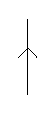
\includegraphics[scale=0.75]{graphics/particleline}
            \caption{Particle line}
        } \qquad
        \parbox{0.35\textwidth}{
            \centering
            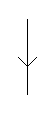
\includegraphics[scale=0.75]{graphics/holeline}
            \caption{Hole line}
        }
    \end{figure}

    \begin{itemize}
        \item Represents a contraction between second quantized operators.
        \item External lines are connected to one operator vertex and infinity.
        \item Internal lines are connected to operator vertices in both ends.
    \end{itemize}

\end{frame}

    

\begin{frame}{Diagram elements - Onebody Hamiltonian}
    \note{Filename: diagram\_hamiltonian01.tex}

    \renewcommand{\figurename}{Level}

    \begin{figure}
    \centering
    \parbox{0.20\textwidth}{
            \centering
            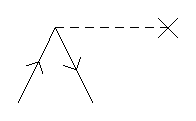
\includegraphics[scale=0.65]{graphics/f1}
            \caption{-1}
        }
        \parbox{0.20\textwidth}{
            \centering
            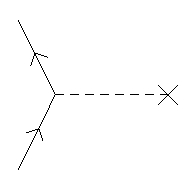
\includegraphics[scale=0.65]{graphics/f2}
            \caption{0}
        }
        \parbox{0.20\textwidth}{
            \centering
            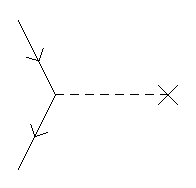
\includegraphics[scale=0.65]{graphics/f3}
            \caption{0}
        }
        \parbox{0.20\textwidth}{
            \centering
            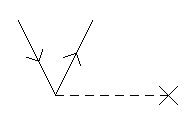
\includegraphics[scale=0.65]{graphics/f4}
            \caption{+1}
        }
    \end{figure}

    \begin{itemize}
        \item Horisontal dashed line segment with one vertex.
        \item Excitation level identify the number of particle/hole pairs created by the operator.
    \end{itemize}
\end{frame}

    

\begin{frame}{Diagram elements - Twobody Hamiltonian}
    \note{Filename: diagram\_hamiltonian02.tex}

    \renewcommand{\figurename}{Level}

    \begin{figure}
    \centering
    \parbox{0.30\textwidth}{
            \centering
            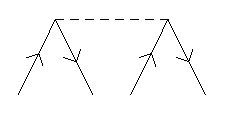
\includegraphics[scale=0.45]{graphics/v1}
            \caption{-2}
        }\quad
        \parbox{0.30\textwidth}{
            \centering
            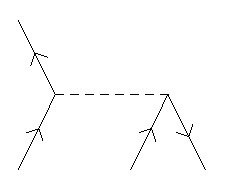
\includegraphics[scale=0.45]{graphics/v2}
            \caption{-1}
        }\quad
        \parbox{0.30\textwidth}{
            \centering
            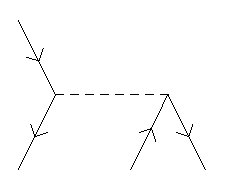
\includegraphics[scale=0.45]{graphics/v3}
            \caption{-1}
        }
    \end{figure}

    \begin{figure}
    \centering
    \parbox{0.30\textwidth}{
            \centering
            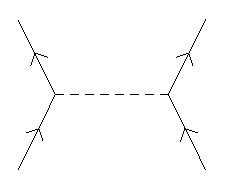
\includegraphics[scale=0.45]{graphics/v4}
            \caption{0}
        }\quad
        \parbox{0.30\textwidth}{
            \centering
            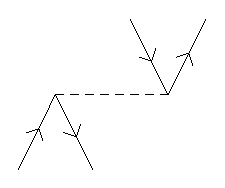
\includegraphics[scale=0.45]{graphics/v5}
            \caption{0}
        }\quad
        \parbox{0.30\textwidth}{
            \centering
            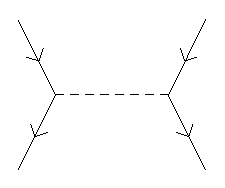
\includegraphics[scale=0.45]{graphics/v6}
            \caption{0}
        }
    \end{figure}

    \begin{figure}
    \centering
    \parbox{0.30\textwidth}{
            \centering
            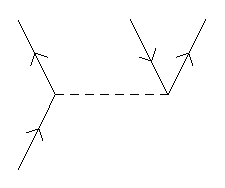
\includegraphics[scale=0.45]{graphics/v7}
            \caption{+1}
        }\quad
        \parbox{0.30\textwidth}{
            \centering
            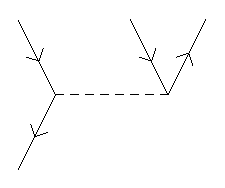
\includegraphics[scale=0.45]{graphics/v8}
            \caption{+1}
        }\quad
        \parbox{0.30\textwidth}{
            \centering
            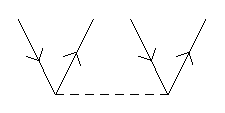
\includegraphics[scale=0.45]{graphics/v9}
            \caption{+2}
        }
    \end{figure}

\end{frame}

    

\begin{frame}{Diagram elements - Onebody cluster operator}
    \note{Filename: diagram\_cc01.tex}

    \renewcommand{\figurename}{Level}

    \begin{figure}
    \centering
    \parbox{0.20\textwidth}{
            \centering
            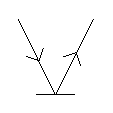
\includegraphics[scale=0.65]{graphics/t1}
            \caption{+1}
        }
    \end{figure}

    \begin{itemize}
        \item Horisontal line segment with one vertex.
        \item Excitation level of +1.
    \end{itemize}
\end{frame}

    

\begin{frame}{Diagram elements - Twobody cluster operator}
    \note{Filename: diagram\_cc02.tex}

    \renewcommand{\figurename}{Level}

    \begin{figure}
    \centering
    \parbox{0.20\textwidth}{
            \centering
            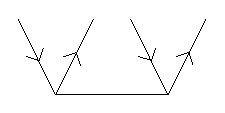
\includegraphics[scale=0.65]{graphics/t2}
            \caption{+2}
        }
    \end{figure}

    \begin{itemize}
        \item Horisontal line segment with two vertices.
        \item Excitation level of +2.
    \end{itemize}
\end{frame}

    

\begin{frame}{CCSD energy equation - Derivation }
    \note{Filename: ccsd\_diagramderivation01.tex}

    \begin{equation*}
        \mathrm{E}_{\mathrm{CCSD}} = \bra{\Phi_0} \barh \ket{\Phi_0}
    \end{equation*}
    \begin{columns}
    \column{0.5\textwidth}
    \begin{itemize}
        \item No external lines.
        \item Final excitation level: 0 
    \end{itemize}
    \column{0.5\textwidth}
    \begin{figure}
        \centering
        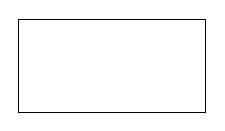
\includegraphics[scale=0.65]{graphics/energy_diag}
    \end{figure}
    \end{columns}
    \renewcommand{\figurename}{Elements}
    \begin{columns}[t]
    \column{0.75\textwidth}
    \begin{figure}
        \caption{$\op{H}_N$}
        \centering
        \parbox{0.20\textwidth}{
            \centering
            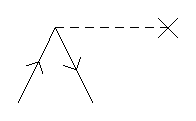
\includegraphics[scale=0.35]{graphics/f1}} 
        \parbox{0.20\textwidth}{
            \centering
            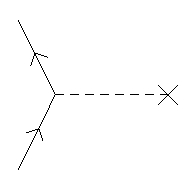
\includegraphics[scale=0.35]{graphics/f2}} 
        \parbox{0.20\textwidth}{
            \centering
            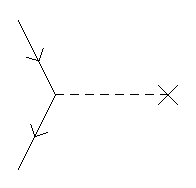
\includegraphics[scale=0.35]{graphics/f3}} 
        \parbox{0.20\textwidth}{
            \centering
            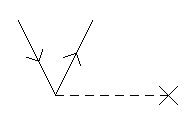
\includegraphics[scale=0.35]{graphics/f4}} 
        \parbox{0.20\textwidth}{
            \centering
            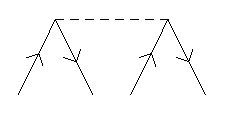
\includegraphics[scale=0.35]{graphics/v1}} 
        \parbox{0.20\textwidth}{
            \centering
            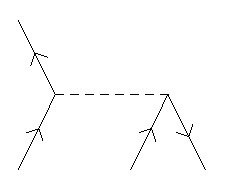
\includegraphics[scale=0.35]{graphics/v2}} 
        \parbox{0.20\textwidth}{
            \centering
            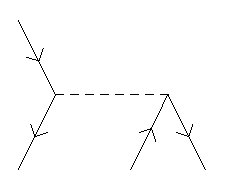
\includegraphics[scale=0.35]{graphics/v3}} 
        \parbox{0.20\textwidth}{
            \centering
            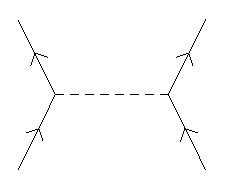
\includegraphics[scale=0.35]{graphics/v4}} 
        \parbox{0.20\textwidth}{
            \centering
            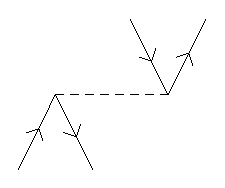
\includegraphics[scale=0.35]{graphics/v5}} 
        \parbox{0.20\textwidth}{
            \centering
            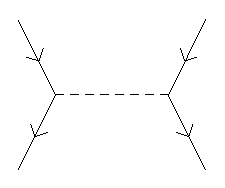
\includegraphics[scale=0.35]{graphics/v6}} 
        \parbox{0.20\textwidth}{
            \centering
            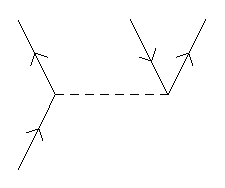
\includegraphics[scale=0.35]{graphics/v7}} 
        \parbox{0.20\textwidth}{
            \centering
            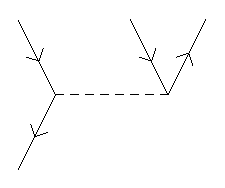
\includegraphics[scale=0.35]{graphics/v8}} 
        \parbox{0.20\textwidth}{
            \centering
            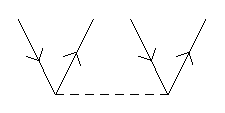
\includegraphics[scale=0.35]{graphics/v9}} 
    \end{figure}
    \column{0.25\textwidth}
    \begin{figure}
        \caption{$\op{T}$}
        \centering
        \parbox[height=3cm]{0.60\textwidth}{
            \centering
            \includegraphics[scale=0.45]{graphics/t1}} 
    \end{figure}
    \begin{figure}
        \parbox[height=3cm]{0.60\textwidth}{
            \centering
            \includegraphics[scale=0.45]{graphics/t2}} 
    \end{figure}
\end{columns}


\end{frame}

    

\begin{frame}{CCSD energy equation }
    \note{Filename: ccsd\_diagramequations01.tex}
    \begin{equation*}
    E_{CCSD} = 
    \parbox{15mm}{\includegraphics[scale=0.5]{graphics/ccsd_e1}}
    + \parbox{15mm}{\includegraphics[scale=0.5]{graphics/ccsd_e2}}
    + \parbox{15mm}{\includegraphics[scale=0.5]{graphics/ccsd_e3}}
\end{equation*}



\end{frame}

    

\begin{frame}{Diagram rules }
    \note<6>{Filename: diagram\_rules01.tex}

    \begin{itemize}
        \item Label all lines. \pause
        \item Sum over all internal indices. \pause
        \item Extract matrix elements. 
            ($f_{\mathrm{in}}^{\mathrm{out}}$, 
            $\bra{\mathrm{lout, rout}}\ket{\mathrm{lin, rin}}$) \pause
        \item Extract cluster amplitudes with indices in the order left to right. Incoming lines are subscripts, while outgoing lines are superscripts. ($t_{\mathrm{in}}^{\mathrm{out}}$,
                        $t^{\mathrm{lout, rout}}_{\mathrm{lin, rin}}$)\pause
        \item Calculate the phase: $(-1)^{\mathrm{holelines} + \mathrm{loops}}$ \pause
        \item Multiply by a factor of $\frac{1}{2}$ for each equivalent line and each ecuivalent vertex.
    \end{itemize}

\end{frame}

    


\begin{frame}{CCSD energy equation }
    \note{Filename: ccsd\_algebraicequations02.tex}
    \begin{equation*}
    E_{CCSD} = 
    f_a^i t_i^a + \frac{1}{4} \bra{ij}\ket{ab} t_{ij}^{ab} + \frac{1}{2} \bra{ij}\ket{ab}  t_i^a  t_j^b
\end{equation*}

Note the implicit sum over repeated indices.



\end{frame}

    



\begin{frame}{CCSD $\op{T}_1$ amplitude equation - Derivation }
    \note{Filename: ccsd\_diagramderivation02.tex}

    \small
    \begin{equation*}
        0 = \bra{\Phi_i^a} \barh \ket{\Phi_0}
    \end{equation*}
    \begin{columns}
    \column{0.5\textwidth}
    \begin{itemize}
        \item One pair of particle/hole  external lines.
        \item Final excitation level: +1
    \end{itemize}
    \column{0.5\textwidth}
    \begin{figure}
        \centering
        \includegraphics[scale=0.45]{graphics/t1amp_diag}
    \end{figure}
    \end{columns}
    \renewcommand{\figurename}{Elements}
    \begin{columns}[t]
    \column{0.75\textwidth}
    \begin{figure}
        \caption{$\op{H}_N$}
        \centering
        \parbox{0.20\textwidth}{
            \centering
            \includegraphics[scale=0.35]{graphics/f1}} 
        \parbox{0.20\textwidth}{
            \centering
            \includegraphics[scale=0.35]{graphics/f2}} 
        \parbox{0.20\textwidth}{
            \centering
            \includegraphics[scale=0.35]{graphics/f3}} 
        \parbox{0.20\textwidth}{
            \centering
            \includegraphics[scale=0.35]{graphics/f4}} 
        \parbox{0.20\textwidth}{
            \centering
            \includegraphics[scale=0.35]{graphics/v1}} 
        \parbox{0.20\textwidth}{
            \centering
            \includegraphics[scale=0.35]{graphics/v2}} 
        \parbox{0.20\textwidth}{
            \centering
            \includegraphics[scale=0.35]{graphics/v3}} 
        \parbox{0.20\textwidth}{
            \centering
            \includegraphics[scale=0.35]{graphics/v4}} 
        \parbox{0.20\textwidth}{
            \centering
            \includegraphics[scale=0.35]{graphics/v5}} 
        \parbox{0.20\textwidth}{
            \centering
            \includegraphics[scale=0.35]{graphics/v6}} 
        \parbox{0.20\textwidth}{
            \centering
            \includegraphics[scale=0.35]{graphics/v7}} 
        \parbox{0.20\textwidth}{
            \centering
            \includegraphics[scale=0.35]{graphics/v8}} 
        \parbox{0.20\textwidth}{
            \centering
            \includegraphics[scale=0.35]{graphics/v9}} 
    \end{figure}
    \column{0.25\textwidth}
    \begin{figure}
        \caption{$\op{T}$}
        \centering
        \parbox[height=3cm]{0.60\textwidth}{
            \centering
            \includegraphics[scale=0.45]{graphics/t1}} 
    \end{figure}
    \begin{figure}
        \parbox[height=3cm]{0.60\textwidth}{
            \centering
            \includegraphics[scale=0.45]{graphics/t2}} 
    \end{figure}
\end{columns}


\end{frame}

    

\begin{frame}{CCSD $\op{T}_1$ amplitude equation }
    \note{Filename: ccsd\_diagramequations02.tex}

\begin{align*}
    0 &= 
    \parbox{10mm}{\includegraphics[scale=0.4]{graphics/ccsd_hbar_04a}}
    + \parbox{18mm}{\includegraphics[scale=0.4]{graphics/ccsd_hbar_04b}}
    + \parbox{15mm}{\includegraphics[scale=0.4]{graphics/ccsd_hbar_04c}}
    + \parbox{15mm}{\includegraphics[scale=0.4]{graphics/ccsd_hbar_04d}} \\
    & \quad + \parbox{21mm}{\includegraphics[scale=0.4]{graphics/ccsd_hbar_04e}}
    + \parbox{17mm}{\includegraphics[scale=0.4]{graphics/ccsd_hbar_04f}}
    + \parbox{15mm}{\includegraphics[scale=0.4]{graphics/ccsd_hbar_04g}}
    + \parbox{15mm}{\includegraphics[scale=0.4]{graphics/ccsd_hbar_04h}} \\
    & \quad + \parbox{17mm}{\includegraphics[scale=0.4]{graphics/ccsd_hbar_04i}}
    + \parbox{15mm}{\includegraphics[scale=0.4]{graphics/ccsd_hbar_04j}}
    + \parbox{20mm}{\includegraphics[scale=0.4]{graphics/ccsd_hbar_04k}}
    + \parbox{15mm}{\includegraphics[scale=0.4]{graphics/ccsd_hbar_04l}} \\
    & \quad + \parbox{17mm}{\includegraphics[scale=0.4]{graphics/ccsd_hbar_04m}}
    + \parbox{15mm}{\includegraphics[scale=0.4]{graphics/ccsd_hbar_04n}}
\end{align*}

\end{frame}

    

\begin{frame}{Diagram rules }
    \note<6>{Filename: diagram\_rules01.tex}

    \begin{itemize}
        \item Label all lines. \pause
        \item Sum over all internal indices. \pause
        \item Extract matrix elements. 
            ($f_{\mathrm{in}}^{\mathrm{out}}$, 
            $\bra{\mathrm{lout, rout}}\ket{\mathrm{lin, rin}}$) \pause
        \item Extract cluster amplitudes with indices in the order left to right. Incoming lines are subscripts, while outgoing lines are superscripts. ($t_{\mathrm{in}}^{\mathrm{out}}$,
                        $t^{\mathrm{lout, rout}}_{\mathrm{lin, rin}}$)\pause
        \item Calculate the phase: $(-1)^{\mathrm{holelines} + \mathrm{loops}}$ \pause
        \item Multiply by a factor of $\frac{1}{2}$ for each equivalent line and each ecuivalent vertex.
    \end{itemize}

\end{frame}

    


\begin{frame}{CCSD $\op{T}_1$ amplitude equation }
    \note{Filename: ccsd\_algebraicequations02.tex}

\begin{align*}
    0 &= f_{i}^a + f_{e}^a t_i^e - f_{i}^mt_m^a + \bra{ma}\ket{ei} t_m^e 
        + f_{e}^m t_{im}^{ae} + \frac{1}{2} \bra{am}\ket{ef} t_{im}^{ef} \\
        &\, - \frac{1}{2} \bra{mn}\ket{ei} t_{mn}^{ea} - f_{e}^m t_i^e t_m^a
        + \bra{am}\ket{ef} t_i^e t_m^f - \bra{mn}\ket{ei} t_m^e t_n^a  \\
        & \quad + \bra{mn}\ket{ef} t_m^e t_{ni}^{fa}
        - \frac{1}{2} \bra{mn}\ket{ef} t_i^e t_{mn}^{af}
        - \frac{1}{2} \bra{mn}\ket{ef} t_n^a t_{mi}^{ef}\\
        & \quad  - \bra{mn}\ket{ef} t_i^e t_m^a t_n^f
\end{align*}


\end{frame}

    


\begin{frame}{CCSD $\op{T}_2$ amplitude equation - Derivation }
    \note{Filename: ccsd\_diagramderivation03.tex}

    \begin{equation*}
        0 = \bra{\Phi_{ij}^{ab}} \barh \ket{\Phi_0}
    \end{equation*}
    \begin{columns}
    \column{0.5\textwidth}
    \begin{itemize}
        \item Two pairs of particle/hole  external lines.
        \item Final excitation level: +2
    \end{itemize}
    \column{0.5\textwidth}
    \begin{figure}
        \centering
        \includegraphics[scale=0.45]{graphics/t2amp_diag}
    \end{figure}
    \end{columns}
    \renewcommand{\figurename}{Elements}
    \begin{columns}[t]
    \column{0.75\textwidth}
    \begin{figure}
        \caption{$\op{H}_N$}
        \centering
        \parbox{0.20\textwidth}{
            \centering
            \includegraphics[scale=0.35]{graphics/f1}} 
        \parbox{0.20\textwidth}{
            \centering
            \includegraphics[scale=0.35]{graphics/f2}} 
        \parbox{0.20\textwidth}{
            \centering
            \includegraphics[scale=0.35]{graphics/f3}} 
        \parbox{0.20\textwidth}{
            \centering
            \includegraphics[scale=0.35]{graphics/f4}} 
        \parbox{0.20\textwidth}{
            \centering
            \includegraphics[scale=0.35]{graphics/v1}} 
        \parbox{0.20\textwidth}{
            \centering
            \includegraphics[scale=0.35]{graphics/v2}} 
        \parbox{0.20\textwidth}{
            \centering
            \includegraphics[scale=0.35]{graphics/v3}} 
        \parbox{0.20\textwidth}{
            \centering
            \includegraphics[scale=0.35]{graphics/v4}} 
        \parbox{0.20\textwidth}{
            \centering
            \includegraphics[scale=0.35]{graphics/v5}} 
        \parbox{0.20\textwidth}{
            \centering
            \includegraphics[scale=0.35]{graphics/v6}} 
        \parbox{0.20\textwidth}{
            \centering
            \includegraphics[scale=0.35]{graphics/v7}} 
        \parbox{0.20\textwidth}{
            \centering
            \includegraphics[scale=0.35]{graphics/v8}} 
        \parbox{0.20\textwidth}{
            \centering
            \includegraphics[scale=0.35]{graphics/v9}} 
    \end{figure}
    \column{0.25\textwidth}
    \begin{figure}
        \caption{$\op{T}$}
        \centering
        \parbox[height=3cm]{0.60\textwidth}{
            \centering
            \includegraphics[scale=0.45]{graphics/t1}} 
    \end{figure}
    \begin{figure}
        \parbox[height=3cm]{0.60\textwidth}{
            \centering
            \includegraphics[scale=0.45]{graphics/t2}} 
    \end{figure}
\end{columns}


\end{frame}

    
\begin{frame}{CCSD $\op{T}_2$ amplitude equation }
    \note{Filename: ccsd\_diagramequations03.tex}

\begin{align*}
    0 &= 
    \parbox{10mm}{\includegraphics[scale=0.25]{graphics/ccsd_hbar_13_01}} + 
    \parbox{10mm}{\includegraphics[scale=0.25]{graphics/ccsd_hbar_13_02}} + 
    \parbox{10mm}{\includegraphics[scale=0.25]{graphics/ccsd_hbar_13_03}} +
    \parbox{14mm}{\includegraphics[scale=0.25]{graphics/ccsd_hbar_13_04}} + 
    \parbox{14mm}{\includegraphics[scale=0.25]{graphics/ccsd_hbar_13_05}} + 
    \parbox{14mm}{\includegraphics[scale=0.25]{graphics/ccsd_hbar_13_06}} \\
    & + \parbox{14mm}{\includegraphics[scale=0.25]{graphics/ccsd_hbar_13_07}} + 
    \parbox{14mm}{\includegraphics[scale=0.25]{graphics/ccsd_hbar_13_08}} + 
    \parbox{14mm}{\includegraphics[scale=0.25]{graphics/ccsd_hbar_13_09}} +
    \parbox{14mm}{\includegraphics[scale=0.25]{graphics/ccsd_hbar_13_10}} + 
    \parbox{14mm}{\includegraphics[scale=0.25]{graphics/ccsd_hbar_13_11}} \\
    & + \parbox{15mm}{\includegraphics[scale=0.25]{graphics/ccsd_hbar_13_12}} +
    \parbox{19mm}{\includegraphics[scale=0.25]{graphics/ccsd_hbar_13_13}} + 
    \parbox{15mm}{\includegraphics[scale=0.25]{graphics/ccsd_hbar_13_14}} +
    \parbox{15mm}{\includegraphics[scale=0.25]{graphics/ccsd_hbar_13_15}} + 
    \parbox{15mm}{\includegraphics[scale=0.25]{graphics/ccsd_hbar_13_16}} \\
    & + \parbox{15mm}{\includegraphics[scale=0.25]{graphics/ccsd_hbar_13_17}} +
    \parbox{17mm}{\includegraphics[scale=0.25]{graphics/ccsd_hbar_13_18}} + 
    \parbox{15mm}{\includegraphics[scale=0.25]{graphics/ccsd_hbar_13_19}} +
    \parbox{15mm}{\includegraphics[scale=0.25]{graphics/ccsd_hbar_13_20}} + 
    \parbox{15mm}{\includegraphics[scale=0.25]{graphics/ccsd_hbar_13_21}} \\
    & + \parbox{15mm}{\includegraphics[scale=0.25]{graphics/ccsd_hbar_13_22}} + 
    \parbox{15mm}{\includegraphics[scale=0.25]{graphics/ccsd_hbar_13_23}} +
    \parbox{15mm}{\includegraphics[scale=0.25]{graphics/ccsd_hbar_13_24}} + 
    \parbox{15mm}{\includegraphics[scale=0.25]{graphics/ccsd_hbar_13_25}} +
    \parbox{15mm}{\includegraphics[scale=0.25]{graphics/ccsd_hbar_13_26}} \\
    & + \parbox{16mm}{\includegraphics[scale=0.25]{graphics/ccsd_hbar_13_27}} +
    \parbox{17mm}{\includegraphics[scale=0.25]{graphics/ccsd_hbar_13_28}} + 
    \parbox{14mm}{\includegraphics[scale=0.25]{graphics/ccsd_hbar_13_29}} +
    \parbox{15mm}{\includegraphics[scale=0.25]{graphics/ccsd_hbar_13_30}} + 
    \parbox{15mm}{\includegraphics[scale=0.25]{graphics/ccsd_hbar_13_31}}
\end{align*}

\end{frame}

    


\begin{frame}{Diagram rules }
    \begin{itemize}
        \item Label all lines. 
        \item Sum over all internal indices. 
        \item Extract matrix elements. 
            ($f_{\mathrm{in}}^{\mathrm{out}}$, 
            $\bra{\mathrm{lout, rout}}\ket{\mathrm{lin, rin}}$) 
        \item Extract cluster amplitudes with indices in the order left to right. Incoming lines are subscripts, while outgoing lines are superscripts. ($t_{\mathrm{in}}^{\mathrm{out}}$,
                        $t^{\mathrm{lout, rout}}_{\mathrm{lin, rin}}$)
        \item Calculate the phase: $(-1)^{\mathrm{holelines} + \mathrm{loops}}$ 
        \item Multiply by a factor of $\frac{1}{2}$ for each equivalent line and each ecuivalent vertex. 
        \item Antisymmetrize a pair of external particle/hole line that does not connect to the same operator.
    \end{itemize}

\end{frame}

    



\begin{frame}{CCSD $\op{T}_2$ amplitude equation }
    \note{Filename: ccsd\_algebraicequations03.tex}
    \scriptsize
\begin{align*}
    0 &= 
        \bra{ab} \ket{ij}
        + P(ij) \bra{ab}\ket{ej} t_i^e
        - P(ab) \bra{am} \ket{ij} t_m^b
        + P(ab) f_{e}^b t_{ij}^{ae}
        - P(ij) f_{i}^m t_{mj}^{ab} \\
        & + \, \frac{1}{2} \bra{ab}\ket{ef} t_{ij}^{ef}
        + \frac{1}{2} \bra{mn}\ket{ij} t_{mn}^{ab}
        + P(ij) P(ab) \bra{mb}\ket{ej} t_{im}^{ae} \\
        & + \, \frac{1}{2} P(ij) \bra{ab}\ket{ef} t_i^e t_j^f
        + \frac{1}{2} P(ab) \bra{mn}\ket{ij} t_m^a t_n^b
        - P(ij) P(ab) \bra{mb}\ket{ej} t_i^e t_m^a \\
        & + \, \frac{1}{4} \bra{mn}\ket{ef} t_{ij}^{ef} t_{mn}^{ab}
        + \frac{1}{2} P(ij) P(ab) \bra{mn}\ket{ef} t_{im}^{ae} t_{nj}^{fb}
        - \frac{1}{2} P(ab) \bra{mn}\ket{ef} t_{ij}^{ae} t_{mn}^{bf} \\
        & - \, \frac{1}{2} P(ij) \bra{mn}\ket{ef} t_{mi}^{ef} t_{nj}^{ab}
        - P(ij) f_{e}^m t_i^e t_{mj}^{ab}
        - P(ab) f_{e}^m t_{ij}^{ae} t_m^b \\
        & + \, P(ij) P(ab) \bra{am}\ket{ef} t_i^e t_{mj}^{fb}
        - \frac{1}{2} P(ab) \bra{am}\ket{ef} t_{ij}^{ef} t_m^b
        + P(ab) \bra{bm}\ket{ef} t_{ij}^{ae} t_m^f \\
        & - \, P(ij) P(ab) \bra{mn} \ket{ej} t_{im}^{ae} t_n^b
        + \frac{1}{2} P(ij) \bra{mn}\ket{ej} t_i^e t_{mn}^{ab}
        -P(ij) \bra{mn}\ket{ei} t_m^e t_{nj}^{ab} \\
        & - \, \frac{1}{2} P(ij) P(ab) \bra{am}\ket{ef} t_i^e t_j^f t_m^b
        + \frac{1}{2} P(ij) P(ab) \bra{mn}\ket{ej} t_i^e t_m^a t_n^b \\
        & + \, \frac{1}{4} P(ij) \bra{mn}\ket{ef} t_i^e t_{mn}^{ab} t_j^f
        - P(ij) P(ab) \bra{mn}\ket{ef} t_i^e t_m^a t_{nj}^{fb} \\
        & + \, \frac{1}{4} P(ab) \bra{mn}\ket{ef} t_m^a t_{ij}^{ef} t_n^b
        - P(ij) \bra{mn}\ket{ef} t_m^e t_i^f t_{nj}^{ab}
        - P(ab) \bra{mn}\ket{ef} t_{ij}^{ae} t_m^b t_n^f \\
        & + \, \frac{1}{4} P(ij) P(ab) \bra{mn}\ket{ef} t_i^e t_m^a t_j^f t_n^b \\
\end{align*}

\end{frame}

    

\begin{frame}{The $\barh$ expansion}
    \note{Filename: ccsd\_barh\_expansion01.tex}
        \small
        \begin{align*}
            E_{CC} &= \bra{\Psi_0}\Bigl( \hat{H}_N + \left[ \hat{H}_N, \hat{T} \right] +
                \frac{1}{2} \left[\left[ \hat{H}_N, \hat{T} \right], \hat{T}\right]
                + \frac{1}{3!} \left[ \left[\left[ \hat{H}_N, \hat{T} \right], \hat{T}\right], \hat{T} \right] \\
                & \quad + \frac{1}{4!} \left[ \left[ \left[\left[ \hat{H}_N, \hat{T} \right], \hat{T}\right], \hat{T} \right], \hat{T} \right] ++ \Bigr) \ket{\Psi_0} \\
        \end{align*}
        \begin{align*}
            0 &= \bra{\Psi_{ij\ldots}^{ab\ldots}}\Bigl( \hat{H}_N + \left[ \hat{H}_N, \hat{T} \right] +
                \frac{1}{2} \left[\left[ \hat{H}_N, \hat{T} \right], \hat{T}\right]
                + \frac{1}{3!} \left[ \left[\left[ \hat{H}_N, \hat{T} \right], \hat{T}\right], \hat{T} \right] \\
                & \quad + \frac{1}{4!} \left[ \left[ \left[\left[ \hat{H}_N, \hat{T} \right], \hat{T}\right], \hat{T} \right], \hat{T} \right] ++\Bigr) \ket{\Psi_0} \\
        \end{align*}

\end{frame}

    

\begin{frame}{The CCSD energy equation revisited}
    \note{Filename: ccsd\_barh\_expansion02.tex}
        The expanded CC energy equation involves an infinite sum over nested commutators
        \begin{align*}
            E_{CC} &= \bra{\Psi_0}\Bigl( \hat{H}_N + \left[ \hat{H}_N, \hat{T} \right] +
                \frac{1}{2} \left[\left[ \hat{H}_N, \hat{T} \right], \hat{T}\right] \\
                & \qquad + \frac{1}{3!} \left[ \left[\left[ \hat{H}_N, \hat{T} \right], \hat{T}\right], \hat{T} \right] \\
                & \qquad + \frac{1}{4!} \left[ \left[ \left[\left[ \hat{H}_N, \hat{T} \right], \hat{T}\right], \hat{T} \right], \hat{T} \right] ++ \Bigr) \ket{\Psi_0}, \\
        \end{align*}
        but fortunately we can show that it truncates naturally, depending on the Hamiltonian.
        
    \begin{block}{}
        The first term is zero by construction.
        \begin{equation*}
            \bra{\Psi_0} \op{H}_N \ket{\Psi_0} = 0
        \end{equation*}       
    \end{block}
\end{frame}

    

\begin{frame}{The CCSD energy equation revisited.}
    \note{Filename: ccsd\_barh\_expansion03.tex}
     The second term can be split up into different pieces
    \small
        \begin{align*}
        \bra{\Psi_0}\left[ \hat{H}_N, \hat{T} \right]\ket{\Psi_0} & = 
            \bra{\Psi_0} \Bigl(\left[ \hat{F}_N, \hat{T}_1 \right] + \left[ \hat{F}_N, \hat{T}_2 \right]
            + \left[ \hat{V}_N, \hat{T}_1 \right] + \left[ \hat{V}_N, \hat{T}_2 \right] \Bigr) \ket{\Psi_0}
    \end{align*}

    \begin{block}{}
    Since we need the explicit expressions for the commutators both in the next term and in the amplitude equations, we calculate them separately.
    \end{block}

\end{frame}

    

\begin{frame}{The $\barh$ expansion - $\left[ \hat{F}_N, \hat{T}_1 \right]$}
    \note{Filename: ccsd\_barh\_expansion04.tex}
    \begin{align*}
        \left[ \hat{F}_N, \hat{T}_1 \right] &= \sum_{pqia} \left(f_q^p \normord{a_p^\dagger a_q} 
            t_i^a \normord{a_a^\dagger a_i} - t_i^a \normord{a_a^\dagger a_i} f_q^p \normord{a_p^\dagger a_q} \right) \\
        &= \sum_{pqia} f_q^p t_i^a \left( \normord{a_p^\dagger a_q} \normord{a_a^\dagger a_i} -
                \normord{a_a^\dagger a_i} \normord{a_p^\dagger a_q} \right)
    \end{align*} \pause
        \begin{align*}
            \left\{a_a^\dagger a_i\right\} \left\{a_p^\dagger a_q \right\} &= \normord{a_a^\dagger a_i a_p^\dagger a_q} \pause
                = \normord{a_p^\dagger a_q a_a^\dagger a_i} \\ \pause
        \normord{a_p^\dagger a_q}\normord{a_a^\dagger a_i} &= \normord{a_p^\dagger a_q a_a^\dagger a_i}  \\ \pause
            & \quad + \normord{
               \contraction{}{a}{{}^\dagger_pa_q a^\dagger_a}{a}
                a^\dagger_p a_q a^\dagger_a a_i} +
            \normord{
                \contraction{a^\dagger_p}{a}{{}_q}{a}
                a^\dagger_p a_q a^\dagger_a a_i} \\ \pause
            & \quad + \normord{
                \contraction[1.5ex]{}{a}{{}^\dagger_pa_q a^\dagger_a}{a}
                \contraction{a^\dagger_p}{a}{{}_q}{a}
                a^\dagger_p a_q a^\dagger_a a_i} \\ \pause
            &=  \normord{a_p^\dagger a_q a_a^\dagger a_i} + \delta_{qa} \normord{a_p^\dagger a_i} + \delta_{pi} \normord{a_q a_a^\dagger}
            + \delta_{qa}\delta_{pi}
        \end{align*}
\end{frame}

    

\begin{frame}{The $\barh$ expansion - $\left[ \hat{F}_N, \hat{T}_1 \right]$}
    \note{Filename: ccsd\_barh\_expansion05.tex}

        Wicks theorem gives us
        \begin{align*}
            \left\{a_p^\dagger a_q \right\}\left\{a_a^\dagger a_i\right\} - \left\{a_a^\dagger a_i\right\} \left\{a_p^\dagger a_q \right\} &= \delta_{qa} \left\{ a_p^\dagger a_i\right\} + \delta_{pi} \left\{ a_q a_a^\dagger \right\} + \delta_{qa}\delta_{pi}.
    \end{align*}

        Inserted into the original expression, we arrive at the explicit value of the commutator
        \begin{align*}
        \left[ \hat{F}_N, \hat{T}_1 \right] &= \sum_{pai} f_a^p t_i^a \normord{a_p^\dagger a_i} + 
                \sum_{qai} f_q^i t_i^a \normord{a_q a_a^\dagger} + \sum_{ai} f_a^i t_i^a \\
            &= \left( \op{F}_N \op{T}_1 \right)_c.
        \end{align*}
    The subscript means that the product only includes terms where the operators are connected by atleast one shared index.

\end{frame}

    

\begin{frame}{The $\barh$ expansion - $\left[ \hat{F}_N, \hat{T}_2 \right]$}
    \note{Filename: ccsd\_barh\_expansion06.tex}
    \begin{align*}
        \left[ \hat{F}_N, \hat{T}_2 \right] 
        &= \left[\sum_{pq} f_q^p \normord{a^\dagger_p a_q},
            \frac{1}{4}\sum_{ijab} t_{ij}^{ab} \normord{a^\dagger_a a^\dagger_b a_j a_i} \right] \\
        &= \frac{1}{4}\sum_{\substack{pq\\ijab}}
        \left[ \normord{a^\dagger_p a_q}, \normord{a^\dagger_a a^\dagger_b a_j a_i} \right] \\
        &= \frac{1}{4}\sum_{\substack{pq\\ijab}}
            f_q^p t_{ij}^{ab}
        \left( \normord{a^\dagger_p a_q} \normord{a^\dagger_a a^\dagger_b a_j a_i}
            - \normord{a^\dagger_a a^\dagger_b a_j a_i} \normord{a^\dagger_p a_q} \right)
    \end{align*}
\end{frame}

    

\begin{frame}{The $\barh$ expansion - $\left[ \hat{F}_N, \hat{T}_2 \right]$}
    \note{Filename: ccsd\_barh\_expansion07.tex}
    \small
    \begin{align*}
        \normord{a^\dagger_a a^\dagger_b a_j a_i} \normord{a^\dagger_p a_q} &= 
            \normord{a^\dagger_a a^\dagger_b a_j a_i a^\dagger_p a_q} \\ \pause
        &= \normord{a^\dagger_p a_q a^\dagger_a a^\dagger_b a_j a_i} \pause
        \\
        \normord{a^\dagger_p a_q} \normord{a^\dagger_a a^\dagger_b a_j a_i} &= 
            \normord{a^\dagger_p a_q a^\dagger_a a^\dagger_b a_j a_i} \pause
        + \left\{ 
        \contraction{}{a}{{}^\dagger_pa_q a^\dagger_a a^\dagger_b}{a}
        a^\dagger_p a_q a^\dagger_a a^\dagger_b a_j a_i\right\}
        + \left\{ 
        \contraction{}{a}{{}^\dagger_pa_q a^\dagger_a a^\dagger_b a_j}{a}
        a^\dagger_p a_q a^\dagger_a a^\dagger_b a_j a_i\right\} \\
        & \quad 
        + \left\{ 
        \contraction{a^\dagger_p}{a}{{}_q}{a}
        a^\dagger_p a_q a^\dagger_a a^\dagger_b a_j a_i\right\}
        + \left\{ 
        \contraction{a^\dagger_p}{a}{{}_q a^\dagger_a}{a}
        a^\dagger_p a_q a^\dagger_a a^\dagger_b a_j a_i\right\} \pause
        + \left\{ 
        \contraction{a^\dagger_p}{a}{{}_q}{a}
        \contraction[1.5ex]{}{a}{{}^\dagger_pa_q a^\dagger_a a^\dagger_b}{a}
        a^\dagger_p a_q a^\dagger_a a^\dagger_b a_j a_i\right\} \\
        & \quad 
        + \left\{ 
        \contraction{a^\dagger_p}{a}{{}_q}{a}
        \contraction[1.5ex]{}{a}{{}^\dagger_pa_q a^\dagger_a a^\dagger_b a_j}{a}
        a^\dagger_p a_q a^\dagger_a a^\dagger_b a_j a_i\right\}
        + \left\{ 
        \contraction{a^\dagger_p}{a}{{}_q a^\dagger_a}{a}
        \contraction[1.5ex]{}{a}{{}^\dagger_pa_q a^\dagger_a a^\dagger_b}{a}
        a^\dagger_p a_q a^\dagger_a a^\dagger_b a_j a_i\right\}
        + \left\{ 
        \contraction{a^\dagger_p}{a}{{}_q a^\dagger_a}{a}
        \contraction[1.5ex]{}{a}{{}^\dagger_pa_q a^\dagger_a a^\dagger_b a_j}{a}
        a^\dagger_p a_q a^\dagger_a a^\dagger_b a_j a_i\right\} \\ \pause
        &= \normord{a^\dagger_p a_q a^\dagger_a a^\dagger_b a_j a_i}
        - \delta_{pj} \normord{a_q a^\dagger_a a^\dagger_b a_i}
        + \delta_{pi} \normord{a_q a^\dagger_a a^\dagger_b a_j} \\
        & \quad + \delta_{qa} \normord{a^\dagger_p a^\dagger_b a_j a_i}
        - \delta_{qb}\normord{a^\dagger_p a^\dagger_a a_j a_i} 
        - \delta_{pj} \delta_{qa} \normord{a^\dagger_b a_i} \\
        & \quad + \delta_{pi} \delta_{qa} \normord{a^\dagger_b a_j}
        + \delta_{pj} \delta_{qb} \normord{a^\dagger_a a_i}
        - \delta_{pi} \delta_{qb} \normord{a^\dagger_a a_j}
    \end{align*}

\end{frame}

    

\begin{frame}{The $\barh$ expansion - $\left[ \hat{F}_N, \hat{T}_2 \right]$}
    \note{Filename: ccsd\_barh\_expansion08.tex}
    Wicks theorem gives us
    \small
    \begin{align*}
        & \Bigl( \normord{a^\dagger_p a_q} \normord{a^\dagger_a a^\dagger_b a_j a_i}
            - \normord{a^\dagger_a a^\dagger_b a_j a_i} \normord{a^\dagger_p a_q} \Bigr) = \\
        & \qquad - \delta_{pj} \normord{a_q a^\dagger_a a^\dagger_b a_i}
        + \delta_{pi} \normord{a_q a^\dagger_a a^\dagger_b a_j}
        + \delta_{qa} \normord{a^\dagger_p a^\dagger_b a_j a_i} \\
        & \qquad - \delta_{qb}\normord{a^\dagger_p a^\dagger_a a_j a_i} 
        - \delta_{pj} \delta_{qa} \normord{a^\dagger_b a_i}
        + \delta_{pi} \delta_{qa} \normord{a^\dagger_b a_j}
        + \delta_{pj} \delta_{qb} \normord{a^\dagger_a a_i} \\
        & \qquad - \delta_{pi} \delta_{qb} \normord{a^\dagger_a a_j}
    \end{align*}
    \pause
    Inserted into the original expression, we arrive at
    \begin{align*}
        \left[ \op{F}_N, \op{T}_2 \right]
        &= \frac{1}{4} \sum_{\substack{pq\\abij}} f_q^p t_{ij}^{ab} \Bigl(
        - \delta_{pj} \normord{a_q a^\dagger_a a^\dagger_b a_i}
        + \delta_{pi} \normord{a_q a^\dagger_a a^\dagger_b a_j} \\
        & \quad + \delta_{qa} \normord{a^\dagger_p a^\dagger_b a_j a_i}
        - \delta_{qb}\normord{a^\dagger_p a^\dagger_a a_j a_i} 
        - \delta_{pj} \delta_{qa} \normord{a^\dagger_b a_i} \\
        & \quad + \delta_{pi} \delta_{qa} \normord{a^\dagger_b a_j}
        + \delta_{pj} \delta_{qb} \normord{a^\dagger_a a_i}
        - \delta_{pi} \delta_{qb} \normord{a^\dagger_a a_j} \Bigr).
    \end{align*}

\end{frame}

    

\begin{frame}{The $\barh$ expansion - $\left[ \hat{F}_N, \hat{T}_2 \right]$}
    \note{Filename: ccsd\_barh\_expansion09.tex}

    After renaming indices and changing the order of operators, we arrive at the explicit expression
    \begin{align*}
        \left[ \op{F}_N, \op{T}_2 \right]
        &= \frac{1}{2} \sum_{qijab} f_q^i t_{ij}^{ab} \normord{a_q a^\dagger_a a^\dagger_b a_j}
        + \frac{1}{2} \sum_{pijab} f_a^p t_{ij}^{ab} \normord{a^\dagger_p a^\dagger_b a_j a_i} \\
        & \quad + \sum_{ijab} f_a^i t_{ij}^{ab} \normord{a^\dagger_b a_j} \\
    &= \left( \op{F}_N \op{T}_2\right)_c.
    \end{align*}
    The subscript implies that only the connected terms from the product contribute.

\end{frame}

    

\begin{frame}{The $\barh$ expansion - $\frac{1}{2}\left[ \left[ \op{F}_N, \op{T}_1 \right], \op{T}_1 \right]$}
    \note{Filename: ccsd\_barh\_expansion10.tex}
    \small
        \begin{align*}
        \left[ \hat{F}_N, \hat{T}_1 \right] &= \sum_{pai} f_a^p t_i^a \normord{a_p^\dagger a_i} + 
                \sum_{qai} f_q^i t_i^a \normord{a_q a_a^\dagger} + \sum_{ai} f_a^i t_i^a
        \end{align*}

        \pause
    \begin{align*}
        \left[ \left[ \op{F}_N, \op{T}_1 \right], \op{T}_1\right] 
        &= \Bigl[ \sum_{pai} f_a^p t_i^a \normord{a_p^\dagger a_i} +
            \sum_{qai} f_q^i t_i^a \normord{a_q a_a^\dagger} + \sum_{ai} f_a^i t_i^a, \sum_{jb} t_j^b \normord{a_b^\dagger a_j} \\
        &= \Bigl[ \sum_{pai} f_a^p t_i^a \normord{a_p^\dagger a_i} +
            \sum_{qai} f_q^i t_i^a \normord{a_q a_a^\dagger}, \sum_{jb} t_j^b \normord{a_b^\dagger a_j} \\
        &= \sum_{pabij} f_a^p t_i^a t_j^b \left[ \normord{a_p^\dagger a_i}, \normord{a_b^\dagger a_j} \right] +
            \sum_{qabij} f_q^i t_i^a t_j^b \left[ \normord{a_q a_a^\dagger}, \normord{a_b^\dagger a_j} \right]
    \end{align*}
        \pause
    \begin{align*}
        \normord{a_b^\dagger a_j} \normord{a_p^\dagger a_i} &= \normord{a_b^\dagger a_j a_p^\dagger a_i} 
            = \normord{ a_p^\dagger a_i a_b^\dagger a_j} \\
        \pause
        \normord{a_b^\dagger a_j} \normord{a_q a_a^\dagger} &= \normord{ a_b^\dagger a_j a_q a_a^\dagger} 
            =  \normord{ a_q a_a^\dagger a_b^\dagger a_j}
    \end{align*}
\end{frame}

    

\begin{frame}{The $\barh$ expansion - $\left[ \left[ \op{F}_N, \op{T}_1 \right], \op{T}_1 \right]$}
    \note{Filename: ccsd\_barh\_expansion11.tex}

    \small
    \begin{align*}
        \frac{1}{2} \left[ \left[ \op{F}_N, \op{T}_1 \right], \op{T}_1\right] 
        &= \frac{1}{2} \left(\sum_{pabij} f_a^p t_i^a t_j^b \delta_{pj} \normord{a_i a_b^\dagger}
            - \sum_{qabij} f_q^i t_i^a t_j^b \delta_{qb} \normord{a_a^\dagger a_j}\right) \\
        &= -\frac{1}{2} 2 \sum_{abij} f_b^j t_j^a t_i^b \normord{a_a^\dagger a_i} \\
        &= -\sum_{abij} f_b^j t_j^a t_i^b \normord{a_a^\dagger a_i} \\
        &= \frac{1}{2} \left(  \op{F}_N \op{T}_1^2 \right)_c
    \end{align*}

\end{frame}

    

\begin{frame}{The CCSD energy equation revisited }
    \note{Filename: ccsd\_barh\_expansion12.tex}

    \small
    \begin{align*}
        \bra{\Phi_0} \left[ \hat{V}_N, \hat{T}_1 \right] \ket{\Phi_0} &= 
            \bra{\Phi_0}
                \left[ \frac{1}{4} \sum_{pqrs} \bra{pq}\ket{rs} \normord{a^\dagger_p a^\dagger_q a_s  a_r},
                    \sum_{ia} t_i^a \normord{a^\dagger_a a_i} \right] \ket{\Phi_0} \\ \pause
            &= \frac{1}{4}\sum_{\substack{
                pqr \\
                sia}} \bra{pq}\ket{rs} t_i^a \bra{\Phi_0} 
                \left[ \normord{a^\dagger_p a^\dagger_q a_s  a_r}, \normord{a^\dagger_a a_i} \right]
                \ket{\Phi_0} \\ \pause
        &= 0
    \end{align*}



\end{frame}

    

\begin{frame}{The CCSD energy equation revisited }
    \note{Filename: ccsd\_barh\_expansion13.tex}

    \small
    \begin{align*}
        & \bra{\Phi_0} \left[ \hat{V}_N, \hat{T}_2 \right] \ket{\Phi_0}= \\
            & \quad \bra{\Phi_0}
                \left[ \frac{1}{4} \sum_{pqrs} \bra{pq}\ket{rs} \normord{a^\dagger_p a^\dagger_q a_s  a_r},
                    \frac{1}{4}\sum_{ijab} t_{ij}^{ab} \normord{a^\dagger_a a^\dagger_b a_j a_i} \right] \ket{\Phi_0} \\ \pause
            &= \frac{1}{16}\sum_{\substack{
                    pqr \\
                    sijab}} \bra{pq}\ket{rs}t_{ij}^{ab} \bra{\Phi_0} 
                \left[ \normord{a^\dagger_p a^\dagger_q a_s  a_r}, \normord{a^\dagger_a a^\dagger_b a_j a_i} \right]
                \ket{\Phi_0} \\ \pause
            &= \frac{1}{16}\sum_{\substack{
                    pqr \\
                    sijab}} \bra{pq}\ket{rs}t_{ij}^{ab} \bra{\Phi_0}
            \Bigl(
            \left\{
            \contraction{a^\dagger_p a^\dagger_q a_s}{a}{{}_r}{a}
            \contraction[1.25ex]{a^\dagger_p a^\dagger_q}{a}{{}_s a_r a^\dagger_a}{a}
            \contraction[1.50ex]{a^\dagger_p}{a}{{}^\dagger_q a_s a_r a^\dagger_a a^\dagger_b}{a}
            \contraction[1.75ex]{}{a}{{}^\dagger_p a^\dagger_q a_s a_r a^\dagger_a a^\dagger_b a_j}{a}
            a^\dagger_p a^\dagger_q a_s  a_r a^\dagger_a a^\dagger_b a_j a_i \right\}
            + \left\{
            \contraction{a^\dagger_p a^\dagger_q}{a}{{}_s a_r}{a}
            \contraction[1.25ex]{a^\dagger_p a^\dagger_q a_s}{a}{{}_r a^\dagger_p}{a}
            \contraction[1.50ex]{a^\dagger_p}{a}{{}^\dagger_q a_s a_r a^\dagger_a a^\dagger_b}{a}
            \contraction[1.75ex]{}{a}{{}^\dagger_p a^\dagger_q a_s a_r a^\dagger_a a^\dagger_b a_j}{a}
            a^\dagger_p a^\dagger_q a_s  a_r a^\dagger_a a^\dagger_b a_j a_i \right\} \\
            & \quad \left\{
            \contraction{a^\dagger_p a^\dagger_q a_s}{a}{{}_r}{a}
            \contraction[1.25ex]{a^\dagger_p a^\dagger_q}{a}{{}_s a_r a^\dagger_a}{a}
            \contraction[1.5ex]{}{a}{{}^\dagger_p a^\dagger_q a_s a_r a^\dagger_a a^\dagger_b}{a}
            \contraction[1.75ex]{a^\dagger_p}{a}{{}^\dagger_q a_s a_r a^\dagger_a a^\dagger_b a_j}{a}
            a^\dagger_p a^\dagger_q a_s  a_r a^\dagger_a a^\dagger_b a_j a_i \right\}
            + \left\{
            \contraction{a^\dagger_p a^\dagger_q}{a}{{}_s a_r}{a}
            \contraction[1.25ex]{a^\dagger_p a^\dagger_q a_s}{a}{{}_r a^\dagger_p}{a}
            \contraction[1.5ex]{}{a}{{}^\dagger_p a^\dagger_q a_s a_r a^\dagger_a a^\dagger_b}{a}
            \contraction[1.75ex]{a^\dagger_p}{a}{{}^\dagger_q a_s a_r a^\dagger_a a^\dagger_b a_j}{a}
            a^\dagger_p a^\dagger_q a_s  a_r a^\dagger_a a^\dagger_b a_j a_i \right\}
            \Bigr) \ket{\Phi_0} \\ \pause
            &= \frac{1}{4} \sum_{ijab} \bra{ij}\ket{ab} t_{ij}^{ab}
    \end{align*}


\end{frame}

    

\begin{frame}{The CCSD energy equation revisited }
    \note{Filename: ccsd\_barh\_expansion14.tex}

    The CCSD energy get two contributions from $\left(\op{H}_N \op{T}\right)_c$
    \begin{align*}
        E_{CC} & \Leftarrow \bra{\Phi_0} \left[ \hat{H}_N, \hat{T} \right] \ket{\Phi_0} \\
            &= \sum_{ia} f_a^i t_i^a + \frac{1}{4} \sum_{ijab} \bra{ij}\ket{ab} t_{ij}^{ab}
    \end{align*}



\end{frame}

    

\begin{frame}{The CCSD energy equation revisited }
    \note{Filename: ccsd\_barh\_expansion15.tex}

    \begin{align*}
        E_{CC} & \Leftarrow \bra{\Phi_0} \frac{1}{2} \left( \op{H}_N \op{T}^2 \right)_c \ket{\Phi_0}
     \end{align*}
    \pause
    \small
    \begin{align*}
        & \bra{\Phi_0} \frac{1}{2} \left( \op{V}_N \op{T}_1^2 \right)_c \ket{\Phi_0} = \\
            & \quad \frac{1}{8} \sum_{pqrs} \sum_{ijab} \bra{pq}\ket{rs} t_i^a t_j^b 
            \bra{\Phi_0} \left(\normord{a^\dagger_p a^\dagger_q a_s  a_r} 
            \normord{a^\dagger_a a_i} \normord{a^\dagger_b a_j} \right)_c\ket{\Phi_0} \\ \pause
        &= \frac{1}{8} \sum_{pqrs} \sum_{ijab} \bra{pq}\ket{rs} t_i^a t_j^b \bra{\Phi_0} \\
        & \quad \Bigl( 
        \left\{
        \contraction{a^\dagger_p a^\dagger_q a_s}{a}{{}_r}{a}
        \contraction[1.25ex]{a^\dagger_p}{a}{{}^\dagger_q a_s a_r a^\dagger_a}{a}
        \contraction[1.5ex]{a^\dagger_p a^\dagger_q }{a}{{}_s a_r a^\dagger_a a_i}{a}
        \contraction[1.75ex]{}{a}{{}^\dagger_p a^\dagger_q a_s a_r a^\dagger_a a_i a^\dagger_b}{a}
        a^\dagger_p a^\dagger_q a_s  a_r a^\dagger_a a_i a^\dagger_b a_j \right\}
        +\left\{
        \contraction{a^\dagger_p a^\dagger_q}{a}{{}_s a_r}{a}
        \contraction[1.25ex]{a^\dagger_p}{a}{{}^\dagger_q a_s a_r a^\dagger_a}{a}
        \contraction[1.5ex]{a^\dagger_p a^\dagger_q a_s}{a}{{}_r a^\dagger_a a_i}{a}
        \contraction[1.75ex]{}{a}{{}^\dagger_p a^\dagger_q a_s a_r a^\dagger_a a_i a^\dagger_b}{a}
        a^\dagger_p a^\dagger_q a_s  a_r a^\dagger_a a_i a^\dagger_b a_j \right\}
        + \left\{
        \contraction{a^\dagger_p a^\dagger_q a_s}{a}{{}_r}{a}
        \contraction[1.25ex]{}{a}{{}^\dagger_p q^\dagger_q a_s a_r a^\dagger_a}{a}
        \contraction[1.5ex]{a^\dagger_p a^\dagger_q }{a}{{}_s a_r a^\dagger_a a_i}{a}
        \contraction[1.75ex]{a^\dagger_p}{a}{{}^\dagger_q a_s a_r a^\dagger_a a_i a^\dagger_b}{a}
        a^\dagger_p a^\dagger_q a_s  a_r a^\dagger_a a_i a^\dagger_b a_j \right\} \\
        & \quad +\left\{
        \contraction{a^\dagger_p a^\dagger_q}{a}{{}_s a_r}{a}
        \contraction[1.25ex]{}{a}{{}^\dagger_p q^\dagger_q a_s a_r a^\dagger_a}{a}
        \contraction[1.5ex]{a^\dagger_p a^\dagger_q a_s}{a}{{}_r a^\dagger_a a_i}{a}
        \contraction[1.75ex]{a^\dagger_p}{a}{{}^\dagger_q a_s a_r a^\dagger_a a_i a^\dagger_b}{a}
        a^\dagger_p a^\dagger_q a_s  a_r a^\dagger_a a_i a^\dagger_b a_j \right\}
        \Bigr) \ket{\Phi_0} \\ \pause
        &= \frac{1}{2} \sum_{ijab} \bra{ij}\ket{ab} t_i^a t_j^b
    \end{align*}



\end{frame}

    

\begin{frame}{The CCSD energy equation revisited }
    \note{Filename: ccsd\_barh\_expansion16.tex}

    \begin{itemize}
        \item No contractions possible between cluster operators. \pause
        \item Cluster operators need to contract with free indices to the left. \pause
        \item Disconnected parts automatically cancel in the commutator. \pause
        \item Onebody operators can connect to maximum two cluster operators. \pause
        \item Twobody operators can connect to maximum four cluster operators. \pause
        \item Different terms in the $\barh$ expansion contributes to different equations.
    \end{itemize}


\end{frame}

    


\begin{frame}
    \frametitle{Factoring, motivation}
\note{Filename: ccsd\_factoring01.tex}

\small
\begin{block}{Diagram (2.12)}
    \begin{equation*}
        \parbox{40mm}{\includegraphics[scale=0.5]{graphics/ccsd_hbar_13_12}}
        = \frac{1}{4}  \bra{mn}\ket{ef} t_{ij}^{ef} t_{mn}^{ab}
    \end{equation*}
\end{block}
\begin{block}{Diagram (2.26)}
    \begin{equation*}
        \parbox{40mm}{\includegraphics[scale=0.5]{graphics/ccsd_hbar_13_26}}
        = \frac{1}{4} P(ij) \bra{mn}\ket{ef} t_i^e t_{mn}^{ab} t_j^f
    \end{equation*}
\end{block}
\begin{block}{Diagram (2.31)}
    \begin{equation*}
        \parbox{40mm}{\includegraphics[scale=0.5]{graphics/ccsd_hbar_13_31}}
        = \frac{1}{4} P(ij) P(ab) \bra{mn}\ket{ef} t_i^e t_m^a t_j^f t_n^b
    \end{equation*}
\end{block}
\end{frame}


\begin{frame}
    \frametitle{Factoring, motivation}
\note{Filename: ccsd\_factoring02.tex}

\scriptsize
\begin{block}{Diagram (2.12)}
    \begin{equation*}
        \parbox{40mm}{\includegraphics[scale=0.5]{graphics/ccsd_hbar_13_12}}
        = \frac{1}{4}  \bra{mn}\ket{ef} t_{ij}^{ef} t_{mn}^{ab}
    \end{equation*}
\end{block}
Diagram cost: $n_p^4 n_h^4$
\begin{block}{Diagram (2.13) - Factored}
\small
    \begin{align*}
        \parbox{40mm}{\includegraphics[scale=0.5]{graphics/ccsd_hbar_13_12}}
        &= \frac{1}{4}  \bra{mn}\ket{ef} t_{ij}^{ef} t_{mn}^{ab} \nn
        &= \frac{1}{4}  \left(\bra{mn}\ket{ef} t_{ij}^{ef}\right)  t_{mn}^{ab} \nn
        &= \frac{1}{4} X_{ij}^{mn} t_{mn}^{ab}
    \end{align*}
\end{block}
\end{frame}


\begin{frame}
    \frametitle{Factoring, motivation}
\note{Filename: ccsd\_factoring03.tex}

\small
\begin{block}{Diagram (2.26)}
    \begin{align*}
        \parbox{40mm}{\includegraphics[scale=0.5]{graphics/ccsd_hbar_13_26}}
        &= \frac{1}{4} P(ij) \bra{mn}\ket{ef} t_i^e t_{mn}^{ab} t_j^f
    \end{align*}
\end{block}
Diagram cost: $n_p^4 n_h^4$
\begin{block}{Diagram (2.26) - Factored}
    \begin{align*}
        \parbox{40mm}{\includegraphics[scale=0.5]{graphics/ccsd_hbar_13_26}}
        &= \frac{1}{4} P(ij) \bra{mn}\ket{ef} t_i^e t_{mn}^{ab} t_j^f \nn
        &= \frac{1}{4} P(ij) t_{mn}^{ab} t_i^e X_{ej}^{mn} \nn
        &= \frac{1}{4} P(ij) t_{mn}^{ab} Y^{mn}_{ij}
    \end{align*}
\end{block}
\end{frame}



\begin{frame}
    \frametitle{Factoring, motivation}
\note{Filename: ccsd\_factoring04.tex}

\scriptsize
\begin{block}{Diagram (2.31)}
    \begin{align*}
        \parbox{40mm}{\includegraphics[scale=0.5]{graphics/ccsd_hbar_13_31}}
        &= \frac{1}{4} P(ij) P(ab) \bra{mn}\ket{ef} t_i^e t_m^a t_j^f t_n^b
    \end{align*}
\end{block}
Diagram cost: $n_p^4 n_h^4$
\begin{block}{Diagram (2.31) - Factored}
    \begin{align*}
        \parbox{40mm}{\includegraphics[scale=0.4]{graphics/ccsd_hbar_13_31}}
        &= \frac{1}{4} P(ij) P(ab) \bra{mn}\ket{ef} t_i^e t_m^a t_j^f t_n^b \nn
        &= \frac{1}{4} P(ij) P(ab) t_m^a t_n^b t_i^e X_{ej}^{mn} \nn
        &= \frac{1}{4} P(ij) P(ab) t_m^a t_n^b Y_{ij}^{mn} \nn
        &= \frac{1}{4} P(ij) P(ab) t_m^a Z_{ij}^{mb}
    \end{align*}
\end{block}
\end{frame}

\begin{frame}
    \frametitle{Factoring, Classification}
\note{Filename: ccsd\_factoring05.tex}

A diagram is classified by how many hole and particle lines between a $\hat{T}_i$ operator and the interaction ($T_i(p^{np} h^{nh})$).
\begin{block}{Diagram (2.12) Classification}
    \begin{equation*}
        \parbox{40mm}{\includegraphics[scale=0.5]{graphics/ccsd_hbar_13_12}}
        = \frac{1}{4}  \bra{mn}\ket{ef} t_{ij}^{ef} t_{mn}^{ab}
    \end{equation*}
\end{block}
This diagram is classified as $T_2(p^2) \times T_2(h^2)$
\end{frame}



\begin{frame}
    \frametitle{Factoring, Classification}
\note{Filename: ccsd\_factoring06.tex}

\begin{block}{Diagram (2.26)} 
    \begin{equation*}
        \parbox{40mm}{\includegraphics[scale=0.5]{graphics/ccsd_hbar_13_26}}
        = \frac{1}{4} P(ij) \bra{mn}\ket{ef} t_i^e t_{mn}^{ab} t_j^f
    \end{equation*}
\end{block}
This diagram is classified as $T_2(h^2) \times T_1(p) \times T_1(p)$
\begin{block}{Diagram (2.31)} 
    \begin{equation*}
        \parbox{40mm}{\includegraphics[scale=0.5]{graphics/ccsd_hbar_13_31}}
        = \frac{1}{4} P(ij) P(ab) \bra{mn}\ket{ef} t_i^e t_m^a t_j^f t_n^b
    \end{equation*}
\end{block}
This diagram is classified as $T_1(p) \times T_1(p) \times T_1(h) \times T_1(h)$
\end{frame}


\begin{frame}
    \frametitle{Factoring, Classification}
\note{Filename: ccsd\_factoring07.tex}

\begin{block}{\centering Cost of making intermediates}
\begin{center}
\begin{tabular}{|l||c|c|}
    \hline
    Object & CPU cost & Memory cost \\
    \hline
    $T_2(h)$ & $n_p^2 n_h$ & $ n_p^2$ \\
    \hline
    $T_2(h^2)$ & $n_p^2$ & $ n_h^{-2} n_p^2$ \\
    \hline
    $T_2(p)$ & $n_p n_h^2$ & $ n_h^2$ \\
    \hline
    $T_2(ph)$ & $n_p n_h$ & $1$ \\
    \hline
    $T_1(h)$ & $n_p$ & $ n_h^{-1} n_p$ \\
    \hline
    $T_2(ph^2)$ & $n_p$ & $ n_h^{-2}$ \\
    \hline
    $T_2(p^2)$ & $ n_h^2$ & $ n_p^{-2} n_h^2$ \\
    \hline
    $T_1(p)$ & $n_h$ & $ n_p^{-1} n_h$ \\
    \hline
    $T_2(p^2h)$ & $n_h$ & $ n_p^{-2}$ \\
    \hline
    $T_1(ph)$ & $1$ & $ n_p^{-1} n_h^{-1}$ \\
    \hline
\end{tabular}
\end{center}

\end{block}
\end{frame}


\begin{frame}
    \frametitle{Factoring, Classification}
\note{Filename: ccsd\_factoring11.tex}

\begin{block}{Classification of $\hat{T}_1$ diagrams}
\begin{tabular}{|l||l|}
    \hline
    Object & Expression id \\
    \hline
    $T_2(ph)$ & 5, 11\\
    \hline
    $T_1(h)$ & 3, 8, 10, 13, 14\\
    \hline
    $T_2(ph^2)$ & 7, 12\\
    \hline
    $T_1(p)$ & 2, 8, 9, 12, 14 \\
    \hline
    $T_2(p^2h)$ & 6, 13\\
    \hline
    $T_1(ph)$ & 4, 9, 10, 11, 14\\
    \hline
\end{tabular}

\end{block}
\end{frame}



\begin{frame}
    \frametitle{Factoring, Classification}
\note{Filename: ccsd\_factoring08.tex}

\begin{block}{Classification of $\hat{T}_2$ diagrams}
\small
\begin{tabular}{|l||l|}
    \hline
    Object & Expression id \\
    \hline
    $T_2(h)$ & 5, 15, 16, 23, 29 \\
    \hline
    $T_2(h^2)$ & 7, 12, 22, 26 \\
    \hline
    $T_2(p)$ & 4, 14, 17, 20, 30 \\
    \hline
    $T_2(ph)$ & 8, 13, 13, 18, 21, 27 \\
    \hline
    $T_1(h)$ & 3, 10, 10, 11, 17, 19, 21, 24, 25, 25, 27, 28, 28, 30, 31, 31 \\
    \hline
    $T_2(ph^2)$ & 14 \\
    \hline
    $T_2(p^2)$ & 6, 12, 19, 28 \\
    \hline
    $T_1(p)$ & 2, 9, 9, 11, 16, 18, 22, 24, 24, 25, 26, 26, 27, 29, 31, 31 \\
    \hline
    $T_2(p^2h)$ & 15 \\
    \hline
    $T_1(ph)$ & 20, 23, 29, 30 \\
    \hline
\end{tabular}

\end{block}
\end{frame}



\begin{frame}
    \frametitle{Factoring, $T_2(h)$}
\note{Filename: ccsd\_factoring09.tex}

\begin{block}{Contribution to the $\hat{T}_2$ amplitude equation from $T_2(h)$}
\begin{align*}
    T_2(h) & \Leftarrow 
        - P(ij) f_{i}^m t_{mj}^{ab}
        - \frac{1}{2} P(ij) \bra{mn}\ket{ef} t_{mi}^{ef} t_{nj}^{ab}
        - P(ij) f_{e}^m t_i^e t_{mj}^{ab} \nn
        & \quad - P(ij) \bra{mn}\ket{ei} t_m^e t_{nj}^{ab}
        - P(ij) \bra{mn}\ket{ef} t_m^e t_i^f t_{nj}^{ab} \nn
    & = - P(ij) t_{im}^{ab} \Bigl[ 
        f_j^m 
        + \bra{mn}\ket{je} t_n^e
        + \frac{1}{2} \bra{mn}\ket{ef}  t_{jn}^{ef} \nn
        & \quad + t_j^e \Bigl(
            f_e^m 
            + \bra{mn}\ket{ef} t_n^f
        \Bigr)
    \Bigr] \nn
    & = - P(ij) t_{im}^{ab} (\mathrm{\bar{H}3})_j^m
\end{align*}

\end{block}
\end{frame}


\begin{frame}
    \frametitle{Factoring, $T_2(h^2)$}
\note{Filename: ccsd\_factoring10.tex}

\begin{block}{Contribution to the $\hat{T}_2$ amplitude equation from $T_2(h^2)$}
\begin{align*}
    T_2(h^2) & \Leftarrow
        \frac{1}{2} \bra{mn}\ket{ij} t_{mn}^{ab}
        + \frac{1}{4} \bra{mn}\ket{ef} t_{ij}^{ef} t_{mn}^{ab}
        + \frac{1}{2} P(ij) \bra{mn}\ket{ej} t_i^e t_{mn}^{ab} \nn
        & \quad + \frac{1}{4} P(ij) \bra{mn}\ket{ef} t_i^e t_{mn}^{ab} t_j^f \nn
    &= \frac{1}{2} t_{mn}^{ab} \Bigl[
        \bra{mn}\ket{ij}
        + \frac{1}{2} \bra{mn}\ket{ef} t_{ij}^{ef} \nn
        & \quad + P(ij) t_j^e \Bigl(
            \bra{mn}\ket{ie} + \frac{1}{2} \bra{mn}\ket{fe} t_i^f
        \Bigr)
    \Bigr] \nn
    &= \frac{1}{2} t_{mn}^{ab} (\mathrm{\bar{H}9})_{ij}^{mn}
\end{align*}

\end{block}
\end{frame}


\begin{frame}
    \frametitle{Factored $T_1$ amplitude equations}
\note{Filename: ccsd\_factoring12.tex}

\begin{align*}
    0 &= f_{i}^a + \bra{ma}\ket{ei} t_m^e + \frac{1}{2} \bra{am}\ket{ef} t_{im}^{ef}
        + t_i^e (\mathrm{I2a})_e^a - t_m^a (\mathrm{\bar{H}3})_i^m \nn
    & \quad + \frac{1}{2} t_{mn}^{ea} (\mathrm{\bar{H}7})_{ie}^{mn} + t_{im}^{ae} 
        (\mathrm{\bar{H}1})_e^m \nn
\end{align*}

Can be solved by
\begin{enumerate}
\item Matrix inversion for each iteration ($n_p^3 n_h^3$)
\item Extracting diagonal elements ($n_p^3 n_h^2$)
\end{enumerate}
\end{frame}


\begin{frame}
    \frametitle{Factored $T_1$ amplitude equations}
\note{Filename: ccsd\_factoring13.tex}

\begin{align*}
    0 &= f_{i}^a + \bra{ma}\ket{ei} t_m^e + \frac{1}{2} \bra{am}\ket{ef} t_{im}^{ef}
        + t_i^e (\mathrm{I2a})_e^a - t_m^a (\mathrm{\bar{H}3})_i^m \nn
    & \quad + \frac{1}{2} t_{mn}^{ea} (\mathrm{\bar{H}7})_{ie}^{mn} + t_{im}^{ae} 
        (\mathrm{\bar{H}1})_e^m \nn \pause
    &= f_{i}^a + \bra{ma}\ket{ei} t_m^e
        + t_i^a (\mathrm{I2a})_a^a + (1 - \delta_{ea}) t_i^e (\mathrm{I2a})_e^a \nn
    & \quad - t_i^a (\mathrm{\bar{H}3})_i^i - (1 - \delta_{mi}) t_m^a (\mathrm{\bar{H}3})_i^m 
        + \frac{1}{2} \bra{am}\ket{ef} t_{im}^{ef} + \frac{1}{2} t_{mn}^{ea} (\mathrm{\bar{H}7})_{ie}^{mn} \nn
    & \quad + t_{im}^{ae} (\mathrm{\bar{H}1})_e^m \nn \pause
    &= f_{i}^a + t_i^a \Bigl( (\mathrm{I2a})_a^a - (\mathrm{\bar{H}3})_i^i \Bigr)
        + \bra{ma}\ket{ei} t_m^e \nn
    & \quad + (1 - \delta_{ea}) t_i^e (\mathrm{I2a})_e^a - (1 - \delta_{mi}) t_m^a (\mathrm{\bar{H}3})_i^m
        + \frac{1}{2} \bra{am}\ket{ef} t_{im}^{ef} \nn
    & \quad + \frac{1}{2} t_{mn}^{ea} (\mathrm{\bar{H}7})_{ie}^{mn} + t_{im}^{ae} (\mathrm{\bar{H}1})_e^m \nn
\end{align*}
\end{frame}




\begin{frame}
    \frametitle{Factored $T_1$ amplitude equations}
\note{Filename: ccsd\_factoring14.tex}

    Define
\begin{equation*}
    D_i^a = (\mathrm{\bar{H}3})_i^i - (\mathrm{I2a})_a^a,
\end{equation*}
and we get the $T_1$ amplitude equations
\begin{align*}
    D_i^a t_i^a &= 
        f_{i}^a + \bra{ma}\ket{ei} t_m^e+ (1 - \delta_{ea}) t_i^e (\mathrm{I2a})_e^a & \\
    & \quad - (1 - \delta_{mi}) t_m^a (\mathrm{\bar{H}3})_i^m
        + \frac{1}{2} \bra{am}\ket{ef} t_{im}^{ef} \nn
    & \quad + \frac{1}{2} t_{mn}^{ea} (\mathrm{\bar{H}7})_{ie}^{mn} + t_{im}^{ae} (\mathrm{\bar{H}1})_e^m.
\end{align*}
\end{frame}




\begin{frame}
    \frametitle{Factored $T_2$ amplitude equations}
\note{Filename: ccsd\_factoring15.tex}

\begin{align*}
    0 &= \bra{ab} \ket{ij}
        + \frac{1}{2} \bra{ab}\ket{ef} t_{ij}^{ef}
        - P(ij) t_{im}^{ab} (\mathrm{\bar{H}3})_j^m
        + \frac{1}{2} t_{mn}^{ab} (\mathrm{\bar{H}9})_{ij}^{mn} \\
        & \quad + P(ab) t_{ij}^{ae} (\mathrm{\bar{H}2})_e^b
        + P(ij) P(ab) t_{im}^{ae} (\mathrm{I10c})_{ej}^{mb}
        - P(ab) t_m^a (\mathrm{I12a})_{ij}^{mb} \\
        & \quad + P(ij)t_i^e (\mathrm{I}11a)_{ej}^{ab} 
\end{align*}

Can be solved by
\begin{enumerate}
\item Matrix inversion for each iteration ($n_p^6 n_h^6$)
\item Extracting diagonal elements ($n_p^4 n_h^2$)
\end{enumerate}
\end{frame}


\begin{frame}
    \frametitle{Factored $T_2$ amplitude equations}
\note{Filename: ccsd\_factoring16.tex}

Similarily we define
\begin{equation*}
    D_{ij}^{ab} = (\mathrm{\bar{H}3})_i^i + (\mathrm{\bar{H}3})_j^j
        - (\mathrm{\bar{H}2})_a^a - (\mathrm{\bar{H}2})_b^b 
\end{equation*}
and get the $T_2$ amplitude equations
\begin{equation*}
\begin{split}
    D_{ij}^{ab} t_{ij}^{ab} &= 
        \bra{ab} \ket{ij} 
        + \frac{1}{2} \bra{ab}\ket{ef} t_{ij}^{ef}
        - P(ij)(1-\delta_{jm}) t_{im}^{ab} (\mathrm{\bar{H}3})_j^m \\
        & \quad + \frac{1}{2} t_{mn}^{ab} (\mathrm{\bar{H}9})_{ij}^{mn}
        + P(ab) (1-\delta_{be}) t_{ij}^{ae} (\mathrm{\bar{H}2})_e^b \\
        & \quad + P(ij) P(ab) t_{im}^{ae} (\mathrm{I10c})_{ej}^{mb}
        - P(ab) t_m^a (\mathrm{I12a})_{ij}^{mb} \\
        & \quad + P(ij)t_i^e (\mathrm{I}11a)_{ej}^{ab}
\end{split}
\end{equation*}

\end{frame}



\begin{frame}
\frametitle{Coupled Cluster algorithm}
\note{Filename: ccsd\_algorithm01.tex}
\begin{center}
\begin{fmpage}{7.7cm}
\hspace*{0.4cm} Setup modelspace \\ 
\hspace*{0.4cm} Calculate f and v amplitudes \\
\hspace*{0.4cm} $t_i^a \gets 0$; $t_{ij}^{ab} \gets 0$ \\
\hspace*{0.4cm} $E \gets 1$; $E_{old} \gets 0$ \\ \pause
\hspace*{0.4cm} $E_{ref} \gets \sum_{i} \bra{i} \op{t} \ket{i} +
    \frac{1}{2} \sum_{ij} \bra{ij} \op{v} \ket{ij}$ \\ \pause
\hspace*{0.4cm} while not converged $(E - E_{old} > \epsilon)$ \\ \pause
\hspace*{0.8cm} Calculate intermediates \\ \pause
\hspace*{0.8cm} $t_i^a \gets $ calculated value \\
\hspace*{0.8cm} $t_{ij}^{ab} \gets $ calculated value \\ \pause
\hspace*{0.8cm} $E_{old} \gets E$ \\
\hspace*{0.8cm} $E \gets f_a^i t_i^a + \frac{1}{4} \bra{ij}\ket{ab} t_{ij}^{ab} + \frac{1}{2} \bra{ij}\ket{ab}  t_i^a  t_j^b$ \\ \pause
\hspace*{0.4cm} end while \\
\hspace*{0.4cm} $E_{GS} \gets E_{ref} + E$
\end{fmpage}
\end{center}
\end{frame}

%\begin{frame}
\frametitle{Coupled Cluster algorithm}
\note{Filename: ccsd\_algorithm02.tex}

Typical convergence of the $T_2$ amplitudes
\begin{center}
    \includegraphics[scale=0.3]{../graphics/He4-convergence-N2}
\end{center}
\end{frame}






\end{document}



\frame
{
\frametitle{Schr\"odinger picture}
\begin{small}
{\scriptsize
The time-dependent Schr\"odinger equation (or equation of motion) reads
\[
\imath \hbar\frac{\partial }{\partial t}|\Psi_S(t)\rangle = \hat{H}\Psi_S(t)\rangle,
\]
where the subscript $S$ stands for Schr\"odinger here.
A formal solution is given by 
\[
|\Psi_S(t)\rangle = \exp{(-\imath\hat{H}(t-t_0)/\hbar)}|\Psi_S(t_0)\rangle.
\]
The Hamiltonian $\hat{H}$ is hermitian and the exponent represents a unitary 
operator with an operation carried ut on the wave function at a time $t_0$.
}
\end{small}
}

\frame
{
\frametitle{Interaction picture}
\begin{small}
{\scriptsize
Our Hamiltonian is normally written out as the sum of an unperturbed part $\hat{H}_0$ and an interaction part $\hat{H}_I$, that is
\[
\hat{H}=\hat{H}_0+\hat{H}_I.
\]
In general we have $[\hat{H}_0,\hat{H}_I]\ne 0$ since $[\hat{T},\hat{V}]\ne 0$.
We wish now to define a unitary transformation in terms of $\hat{H}_0$ by defining
\[
|\Psi_I(t)\rangle = \exp{(\imath\hat{H}_0t/\hbar)}|\Psi_S(t)\rangle,
\]
which is again a unitary transformation carried out now at the time $t$ on the 
wave function in the Schr\"odinger picture. 
}
\end{small}
}
\frame
{
\frametitle{Interaction picture}
\begin{small}
{\scriptsize
We can easily find the equation of motion by taking the time derivative
\[
\imath \hbar\frac{\partial }{\partial t}|\Psi_I(t)\rangle = -\hat{H}_0\exp{(\imath\hat{H}_0t/\hbar)}\Psi_S(t)\rangle+\exp{(\imath\hat{H}_0t/\hbar)}
\imath \hbar\frac{\partial }{\partial t}\Psi_S(t)\rangle.
\]
}
\end{small}
}
\frame
{
\frametitle{Interaction picture}
\begin{small}
{\scriptsize
Using the definition of the Schr\"odinger equation, we can rewrite the last equation as 
\[
\imath \hbar\frac{\partial }{\partial t}|\Psi_I(t)\rangle = \exp{(\imath\hat{H}_0t/\hbar)}\left[-\hat{H}_0+\hat{H}_0+\hat{H}_I\right]\exp{(-\imath\hat{H}_0t/\hbar)}\Psi_I(t)\rangle,
\]
which gives us
\[
\imath \hbar\frac{\partial }{\partial t}|\Psi_I(t)\rangle = \hat{H}_I(t)\Psi_I(t)\rangle,
\]
 with 
\[
\hat{H}_I(t)=
\exp{(\imath\hat{H}_0t/\hbar)}\hat{H}_I\exp{(-\imath\hat{H}_0t/\hbar)}.
\]
}
\end{small}
}
\frame
{
\frametitle{Interaction picture}
\begin{small}
{\scriptsize
The order of the operators is important since $\hat{H}_0$ and $\hat{H}_I$ do generally not commute.
The expectation value of
an arbitrary operator in the interaction picture can now be written as
\[
\langle \Psi'_S(t)|\hat{O}_S|\Psi_S(t)\rangle = 
\langle \Psi'_I(t) |\exp{(\imath\hat{H}_0t/\hbar)}\hat{O}_I
\exp{(-\imath\hat{H}_0t/\hbar)}|\Psi_I(t)\rangle,
\]
and using the definition
\[
\hat{O}_I(t)=
\exp{(\imath\hat{H}_0t/\hbar)}\hat{O}_I\exp{(-\imath\hat{H}_0t/\hbar)},
\]
we obtain
\[
\langle \Psi'_S(t)|\hat{O}_S|\Psi_S(t)\rangle = 
\langle \Psi'_I(t) |\hat{O}_I(t)|\Psi_I(t)\rangle,
\]
stating that a unitary transformation does not change expectation values!
}
\end{small}
}
\frame
{
\frametitle{Interaction picture}
\begin{small}
{\scriptsize
If the take the time derivative of the operator in the interaction picture we arrive at the following equation of motion
\[
\imath \hbar\frac{\partial }{\partial t}\hat{O}_I(t) = \exp{(\imath\hat{H}_0t/\hbar)}\left[\hat{O}_S\hat{H}_0-\hat{H}_0\hat{O}_S\right]\exp{(-\imath\hat{H}_0t/\hbar)}=\left[\hat{O}_I(t),\hat{H}_0\right].
\]
Here we have used the time-independence of the Schr\"odinger equation
together with the observation that any function of an operator commutes with the operator itself. 
}
\end{small}
}
\frame
{
\frametitle{Interaction picture}
\begin{small}
{\scriptsize
In order to solve the equation of motion equation in the interaction picture, we define a unitary operator
time-development operator $\hat{U}(t,t')$. Later we will derive its
connection with the linked-diagram theorem, which yields a
linked expression for the actual operator. 
The action of the operator on the wave function is
\[
|\Psi_I(t) \rangle = \hat{U}(t,t_0)|\Psi_I(t_0)\rangle,
\]
with the obvious value $\hat{U}(t_0,t_0)=1$.
}
\end{small}
}
\frame
{
\frametitle{Interaction picture}
\begin{small}
{\scriptsize
The time-development operator $U$ has the
properties that
\[
     \hat{U}^{\dagger}(t,t')\hat{U}(t,t')=\hat{U}(t,t')\hat{U}^{\dagger}(t,t')=1,
\]
which implies that $U$ is unitary
\[
     \hat{U}^{\dagger}(t,t')=\hat{U}^{-1}(t,t').
\]
Further,
\[
    \hat{U}(t,t')\hat{U}(t't'')=\hat{U}(t,t'')
\]
and
\[
    \hat{U}(t,t')\hat{U}(t',t)=1,
\]
which leads to
\[
    \hat{U}(t,t')=\hat{U}^{\dagger}(t',t).
\]
}
\end{small}
}


\frame
{
\frametitle{Interaction picture}
\begin{small}
{\scriptsize
Using our definition of Schr\"odinger's equation in the interaction picture, we can then construct the operator $\hat{U}$. We have defined
\[
|\Psi_I(t)\rangle = \exp{(\imath\hat{H}_0t/\hbar)}|\Psi_S(t)\rangle,
\]
which can be rewritten as 
\[
|\Psi_I(t)\rangle = \exp{(\imath\hat{H}_0t/\hbar)}\exp{(-\imath\hat{H}(t-t_0)/\hbar)}|\Psi_S(t_0)\rangle,
\]
or
\[
|\Psi_I(t)\rangle = \exp{(\imath\hat{H}_0t/\hbar)}\exp{(-\imath\hat{H}(t-t_0)/\hbar)}\exp{(-\imath\hat{H}_0t_0/\hbar)}|\Psi_I(t_0)\rangle.
\]
}
\end{small}
}
\frame
{
\frametitle{Interaction picture}
\begin{small}
{\scriptsize
From the last expression we can define
\[
\hat{U}(t,t_0)=\exp{(\imath\hat{H}_0t/\hbar)}\exp{(-\imath\hat{H}(t-t_0)/\hbar)}\exp{(-\imath\hat{H}_0t_0/\hbar)}.
\]
It is then easy to convince oneself that the properties defined above are satisfied by the definition of $\hat{U}$. 
}
\end{small}
}
\frame
{
\frametitle{Interaction picture}
\begin{small}
{\scriptsize
We derive the equation of motion for $\hat{U}$ using the above definition.
This results in
\[
\imath \hbar\frac{\partial }{\partial t}\hat{U}(t,t_0) = \hat{H}_I(t)\hat{U}(t,t_0),
\]
which we integrate from $t_0$ to a time $t$ resulting in
\[
\hat{U}(t,t_0)-\hat{U}(t_0,t_0)=\hat{U}(t,t_0)-1=-\frac{\imath}{\hbar}\int_{t_0}^t dt' \hat{H}_I(t')\hat{U}(t',t_0),
\]
which can be rewritten as
\[
\hat{U}(t,t_0)=1-\frac{\imath}{\hbar}\int_{t_0}^t dt' \hat{H}_I(t')\hat{U}(t',t_0).
\]
}
\end{small}
}
\frame
{
\frametitle{Interaction picture}
\begin{small}
{\scriptsize
We can solve this equation iteratively keeping in mind the time-ordering of the of the operators
\[
\hat{U}(t,t_0)=1-\frac{\imath}{\hbar}\int_{t_0}^t dt' \hat{H}_I(t')+\left(\frac{-\imath}{\hbar}\right)^2\int_{t_0}^t dt'\int_{t_0}^{t'} dt'' \hat{H}_I(t')\hat{H}_I(t'')+\dots
\]
The third term can be written as 
\[
\int_{t_0}^t dt'\int_{t_0}^{t'} dt'' \hat{H}_I(t')\hat{H}_I(t'')=
\frac{1}{2}\int_{t_0}^t dt'\int_{t_0}^{t'} dt'' \hat{H}_I(t')\hat{H}_I(t'')
+\frac{1}{2}\int_{t_0}^t dt''\int_{t''}^{t} dt' \hat{H}_I(t')\hat{H}_I(t'').
\]
}
\end{small}
}
\frame
{
\frametitle{Interaction picture}
\begin{small}
{\scriptsize
We obtain this expression by changing the integration order in the second term
via a change of the integration variables $t'$ and $t''$  in 
\[
\frac{1}{2}\int_{t_0}^t dt'\int_{t_0}^{t'} dt'' \hat{H}_I(t')\hat{H}_I(t'').
\]
We can rewrite the terms which contain the double integral as
\[
\int_{t_0}^t dt'\int_{t_0}^{t'} dt'' \hat{H}_I(t')\hat{H}_I(t'')=\]
\[
\frac{1}{2}\int_{t_0}^t dt'\int_{t_0}^{t'} dt''\left[\hat{H}_I(t')\hat{H}_I(t'')\Theta(t'-t'')
+\hat{H}_I(t')\hat{H}_I(t'')\Theta(t''-t')\right],
\]
with $\Theta(t''-t')$ being the standard Heavyside or step function. The step function allows us to give a specific time-ordering to the above expression.
}
\end{small}
}
\frame
{
\frametitle{Interaction picture}
\begin{small}
{\scriptsize
With the $\Theta$-function we can rewrite the last expression as 
\[
\int_{t_0}^t dt'\int_{t_0}^{t'} dt'' \hat{H}_I(t')\hat{H}_I(t'')=
\frac{1}{2}\int_{t_0}^t dt'\int_{t_0}^{t'} dt''\hat{T}\left[\hat{H}_I(t')\hat{H}_I(t'')\right],
\]
where $\Hat{T}$ is the so-called time-ordering operator. 
}
\end{small}
}
\frame
{
\frametitle{Interaction picture}
\begin{small}
{\scriptsize
With this definition, we can rewrite the expression for $\hat{U}$ as 
\[
\hat{U}(t,t_0)=\sum_{n=0}^{\infty}\left(\frac{-\imath}{\hbar}\right)^n\frac{1}{n!}
\int_{t_0}^t dt_1\dots \int_{t_0}^t dt_N \hat{T}\left[\hat{H}_I(t_1)\dots\hat{H}_I(t_n)\right]=\hat{T}\exp{\left[\frac{-\imath}{\hbar}
\int_{t_0}^t dt' \hat{H}_I(t')\right]}.
\]
The above time-evolution operator in the interaction picture will be used
to derive various contributions to many-body perturbation theory. See also exercise 26 for a discussion of the various time orderings.
}
\end{small}
}

\frame
{
\frametitle{Heisenberg picture}
\begin{small}
{\scriptsize
We wish now to define a unitary transformation in terms of $\hat{H}$ by defining
\[
|\Psi_H(t)\rangle = \exp{(\imath\hat{H}t/\hbar)}|\Psi_S(t)\rangle,
\]
which is again a unitary transformation carried out now at the time $t$ on the 
wave function in the Schr\"odinger picture. If we combine this equation with 
Schr\"odinger's equation we obtain the following equation of motion
\[
\imath \hbar\frac{\partial }{\partial t}|\Psi_H(t)\rangle = 0,
\]
meaning that $|\Psi_H(t)\rangle$ is time independent. An operator in this picture is defined as
\[
\hat{O}_H(t)=
\exp{(\imath\hat{H}t/\hbar)}\hat{O}_S\exp{(-\imath\hat{H}t/\hbar)}.
\]
}
\end{small}
}
\frame
{
\frametitle{Heisenberg picture}
\begin{small}
{\scriptsize
The time dependence is then in the operator itself, and this yields in turn the
following equation of motion
\[
\imath \hbar\frac{\partial }{\partial t}\hat{O}_H(t) = \exp{(\imath\hat{H}t/\hbar)}\left[\hat{O}_H\hat{H}-\hat{H}\hat{O}_H\right]\exp{(-\imath\hat{H}t/\hbar)}=\left[\hat{O}_H(t),\hat{H}\right].
\]
We note that an operator in the Heisenberg picture can be related to the corresponding
operator in the interaction picture as 
\[
\hat{O}_H(t)=
\exp{(\imath\hat{H}t/\hbar)}\hat{O}_S\exp{(-\imath\hat{H}t/\hbar)}=\]
\[
\exp{(\imath\hat{H}_It/\hbar)}\exp{(-\imath\hat{H}_0t/\hbar)}\hat{O}_I\exp{(\imath\hat{H}_0t/\hbar)}\exp{(-\imath\hat{H}_It/\hbar)}.
\]
}
\end{small}
}
\frame
{
\frametitle{Heisenberg picture}
\begin{small}
{\scriptsize
With our definition of the time evolution operator we see that
\[
\hat{O}_H(t)=\hat{U}(0,t)\hat{O}_I\hat{U}(t,0),
\]
which in turn implies that $\hat{O}_S=\hat{O}_I(0)=\hat{O}_H(0)$, all operators are equal at $t=0$. The wave function in the Heisenberg formalism is 
related to the other pictures as 
\[
|\Psi_H\rangle=|\Psi_S(0)\rangle=|\Psi_I(0)\rangle,
\]
since the wave function in the Heisenberg picture is time independent. 
We can relate this wave function to that a given time $t$ via the time evolution operator as
\[
|\Psi_H\rangle=\hat{U}(0,t)|\Psi_I(t)\rangle.
\]
}
\end{small}
}



\frame
{
\frametitle{Adiabatic hypothesis}
\begin{small}
{\scriptsize
We assume that the interaction term is switched on gradually. Our wave function at time $t=-\infty$ and $t=\infty$ is supposed to represent a non-interacting system
given by the solution to the unperturbed part of our Hamiltonian $\hat{H}_0$.
We assume the ground state is given by $|\Phi_0\rangle$, which could be a Slater determinant.

We define our Hamiltonian as
\[
\hat{H}=\hat{H}_0+\exp{(-\varepsilon t/\hbar)}\hat{H}_I,
\]
where $\varepsilon$ is a small number. The way we write the Hamiltonian 
and its interaction term is meant to simulate the switching of the interaction.
}
\end{small}
}


\frame
{
\frametitle{Adiabatic hypothesis}
\begin{small}
{\scriptsize
The time evolution of the wave function in the interaction picture is then
\[
|\Psi_I(t) \rangle = \hat{U}_{\varepsilon}(t,t_0)|\Psi_I(t_0)\rangle,
\]
with 
\[
\hat{U}_{\varepsilon}(t,t_0)=\sum_{n=0}^{\infty}\left(\frac{-\imath}{\hbar}\right)^n\frac{1}{n!}
\int_{t_0}^t dt_1\dots \int_{t_0}^t dt_N \exp{(-\varepsilon(t_1+\dots+t_n)/\hbar)}\hat{T}\left[\hat{H}_I(t_1)\dots\hat{H}_I(t_n)\right]
\]

}
\end{small}
}

\frame
{
\frametitle{Adiabatic hypothesis}
\begin{small}
{\scriptsize
In the limit $t_0\rightarrow -\infty$, the solution ot Schr\"odinger's equation is
$|\Phi_0\rangle$, and the eigenenergies are given by 
\[
\hat{H}_0|\Phi_0\rangle=W_0|\Phi_0\rangle,
\]
meaning that 
\[
|\Psi_S(t_0)\rangle = \exp{(-\imath W_0t_0/\hbar)}|\Phi_0\rangle,
\]
with the corresponding interaction picture wave function given by
\[
|\Psi_I(t_0)\rangle = \exp{(\imath \hat{H}_0t_0/\hbar)}|\Psi_S(t_0)\rangle=|\Phi_0\rangle.
\]
}
\end{small}
}


\frame
{
\frametitle{Adiabatic hypothesis}
\begin{small}
{\scriptsize
The solution becomes time independent in the limit $t_0\rightarrow -\infty$.
The same conclusion can be reached by looking at 
\[
\imath \hbar\frac{\partial }{\partial t}|\Psi_I(t)\rangle =
\exp{(\varepsilon |t|/\hbar)}\hat{H}_I|\Psi_I(t)\rangle 
\]
and taking the limit $t\rightarrow -\infty$.
We can rewrite the equation for the wave function at a time $t=0$ as
\[
|\Psi_I(0) \rangle = \hat{U}_{\varepsilon}(0,-\infty)|\Phi_0\rangle.
\]
}
\end{small}
}

\frame
{
\frametitle{Goldstone's theorem and Gell-Mann and Low theorem on the ground state}
\begin{small}
{\scriptsize
Our wave function for ground state (after Gell-Mann and Low, see Phys.~Rev.~{\bf 84}, 350 (1951)) is then
\[
        \frac{\ket{\Psi_0}}{\left\langle\Phi_0 | \Psi_0 \right\rangle}=
    \lim_{\epsilon \rightarrow 0}
   \lim_{t'\rightarrow -\infty}
   \frac{U(0,-\infty )\ket{\Phi_0} }
   { \bra{\Phi_0} U(0,-\infty )\ket{\Phi_0} },
\]
and we ask whether this quantity exists to all orders in perturbation theory.
Goldstone's theorem states that only linked diagrams enter the expression for the final binding energy. It means that energy difference reads now
\[
\Delta E=\sum_{i=0}^{\infty}\langle \Phi_0|\hat{H}_I\left\{\frac{\hat{Q}}{W_0-\hat{H}_0}\hat{H}_I\right\}^i|\Phi_0\rangle_L,
\]
where the subscript $L$ indicates that only linked diagrams are included. In our Rayleigh-Schr\"odinger expansion, the energy difference included also unlinked diagrams. 

}
\end{small}
}

\frame
{
\frametitle{Goldstone's theorem and Gell-Mann and Low theorem on the ground state}
\begin{small}
{\scriptsize
If it does, Gell-Mann and Low showed that it is an eigenstate of $\hat{H}$ with eigenvalue
\[
 \hat{H}\frac{\ket{\Psi_0}}{\left\langle\Phi_0 | \Psi_0 \right\rangle}= E\frac{\ket{\Psi_0}}{\left\langle\Phi_0 | \Psi_0 \right\rangle}
\]
and multiplying from the left with $\langle \Phi_0|$ we can rewrite the last equation
as
\[
E-W_0=\frac{\langle \Phi_0|\hat{H}_I\ket{\Psi_0}}{\left\langle\Phi_0 | \Psi_0 \right\rangle},
\]
since $\hat{H}_0|\Phi_0\rangle = W_0|\Phi_0\rangle$. The numerator and the denominators of the last equation do not exist separately. The theorem of Gell-Mann and Low asserts that this ratio exists. 
}
\end{small}
}


\frame
{
\frametitle{Goldstone's theorem and Gell-Mann and Low theorem on the ground state}
\begin{small}
{\scriptsize
We wish to link the above expression with the corresponding expression from time-dependent perturbation theory. We write our expression as
\[
E-W_0=\Delta E= \lim_{\epsilon \rightarrow 0^+}
   \frac{\bra{\Phi_0(0)}\hat{H}_IU_{\epsilon }(0,-\infty )\ket{\Phi_0(-\infty)} }
   { \bra{\Phi_0(0)} U_{\epsilon}(0,-\infty )\ket{\Phi_0(-\infty)} },
\]
with a numerator 
\[
N=\lim_{\epsilon \rightarrow 0^+}\bra{\Phi_0(0)}\hat{H}_IU_{\epsilon}(0,-\infty )\ket{\Phi_0(-\infty)}, 
\]
which we rewrite as
\[
 N=\lim_{\epsilon \rightarrow 0^+}\bra{\Phi_0(0)}\hat{H}_I(t=0)\displaystyle\sum_{n=0}^{\infty}\frac{(-i)^n}{n!}
   \int_{-\infty}^{0}dt_1  \int_{-\infty}^{0}dt_2\dots  \int_{-\infty}^{0}dt_n}\exp{(\epsilon/\hbar(t_1+\dots+t_n))} \hat{T}\left[H_1(t_1)H_1(t_2)\dots H_1(t_n)\right] \ket{\Phi_0(-\infty)}. 
\]
}
\end{small}
}



\frame
{
\frametitle{Goldstone's theorem and Gell-Mann and Low theorem on the ground state}
\begin{small}
{\scriptsize
A linked diagram (or connected diagram) is a diagram which is linked to the last interaction vertex at $t=0$.
We divide the diagrams into linked and unlinked. 
In general, the way we can distribute $\mu$ unlinked diagrams among the total of $n$ diagrams is given by the combinatorial factor
\[
\left(\begin{array}{c} n \\ \mu \end{array}\right) = \frac{n!}{\mu!\nu!},
\]
and using the following relation
\[
\sum_{n=0}^{\infty}\frac{1}{n!}\sum_{\mu+\nu=n}^{\infty}\frac{n!}{\mu!\nu!}=\sum_{\mu=0}^{\infty}\frac{1}{\mu!}\sum_{\nu}^{\infty}\frac{1}{\nu!},
\]
we can rewrite the numerator $N$ as 
\[
N=\bra{\Phi_0(0)}\hat{H}_IU_{\epsilon}(0,-\infty )\ket{\Phi_0(-\infty)}_L\bra{\Phi_0(0)}U_{\epsilon}(0,-\infty )\ket{\Phi_0(-\infty)},  
=N_LD,
\]
with $N_L$ now containing only linked terms
\[
 N_L=\lim_{\epsilon \rightarrow 0^+}\bra{\Phi_0(0)}\hat{H}_I(t=0)\displaystyle\sum_{\nu=0}^{\infty}\frac{(-i)^{\nu}}{\nu!}
   \int_{-\infty}^{0}dt_1  \int_{-\infty}^{0}dt_2\dots  \int_{-\infty}^{0}dt_n}\exp{(\epsilon/\hbar(t_1+\dots+t_n))} \hat{T}\left[H_1(t_1)H_1(t_2)\dots H_1(t_n)\right] \ket{\Phi_0(-\infty)}_L, 
\]
with the subscript $L$ indicating that only linked diagrams appear, that is those diagrams which are linked to the last interaction vertex.
}
\end{small}
}

\frame
{
\frametitle{Goldstone's theorem and Gell-Mann and Low theorem on the ground state}
\begin{small}
{\scriptsize
A linked diagram (or connected diagram) is a diagram which is linked to the last interaction vertex at $t=0$.
We divide the diagrams into linked and unlinked. 
In general, the way we can distribute $\mu$ unlinked diagrams among the total of $n$ diagrams is given by the combinatorial factor
\[
\left(\begin{array}{c} n \\ \mu \end{array}\right) = \frac{n!}{\mu!\nu!},
\]
and using the following relation
\[
\sum_{n=0}^{\infty}\frac{1}{n!}\sum_{\mu+\nu=n}^{\infty}\frac{n!}{\mu!\nu!}=\sum_{\mu=0}^{\infty}\frac{1}{\mu!}\sum_{\nu}^{\infty}\frac{1}{\nu!},
\]
we can rewrite the numerator $N$ as 
\[
N=\bra{\Phi_0(0)}\hat{H}_IU_{\epsilon}(0,-\infty )\ket{\Phi_0(-\infty)}_L\bra{\Phi_0(0)}U_{\epsilon}(0,-\infty )\ket{\Phi_0(-\infty)},  
=N_LD,
\]
with $N_L$ now containing only linked terms
\[
 N_L=\lim_{\epsilon \rightarrow 0^+}\bra{\Phi_0(0)}\hat{H}_I(t=0)\displaystyle\sum_{\nu=0}^{\infty}\frac{(-i)^{\nu}}{\nu!}
   \int_{-\infty}^{0}dt_1  \int_{-\infty}^{0}dt_2\dots  \int_{-\infty}^{0}dt_n}\exp{(\epsilon/\hbar(t_1+\dots+t_n))} \hat{T}\left[H_1(t_1)H_1(t_2)\dots H_1(t_n)\right] \ket{\Phi_0(-\infty)}_L, 
\]
with the subscript $L$ indicating that only linked diagrams appear, that is those diagrams which are linked to the last interaction vertex.
}
\end{small}
}




\frame
{
\frametitle{Goldstone's theorem and Gell-Mann and Low theorem on the ground state}
\begin{small}
{\scriptsize
We note that also that the term $D$ is nothing but the denominator of the equation for the energy. We obtain then the following expression for the energy
\[
E-W_0=\Delta E=N_L= \bra{\Phi_0(0)}\hat{H}_IU_{\epsilon}(0,-\infty )\ket{\Phi_0(-\infty)}_L,
\]
and Goldstone's theorem is then proved. 
The corresponding expression from Rayleigh-Schr\"odinger perturbation theory is given by
\[
\Delta E=\langle \Phi_0|\left(\hat{H}_I+\hat{H}_I\frac{\hat{Q}}{W_0-\hat{H}_0}\hat{H}_I+
\hat{H}_I\frac{\hat{Q}}{W_0-\hat{H}_0}\hat{H}_I\frac{\hat{Q}}{W_0-\hat{H}_0}\hat{H}_I+\dots\right)|\Phi_0\rangle_C.
\]
}
\end{small}
}


\frame
{
\frametitle{Goldstone's theorem and Gell-Mann and Low theorem on the ground state}
\begin{small}
{\scriptsize
An important point in the derivation of the Gell-Mann and Low theorem
\[
E-W_0=\frac{\langle \Phi_0|\hat{H}_I\ket{\Psi_0}}{\left\langle\Phi_0 | \Psi_0 \right\rangle},
\]
is that the numerator and the denominators of the last equation do not exist separately. The theorem of Gell-Mann and Low asserts that this ratio exists. To prove it we proceed as follows. Consider the expression
\[
(\hat{H}_0-E)U_{\epsilon }(0,-\infty )\ket{\Phi_0}=\left[\hat{H}_0,U_{\epsilon }(0,-\infty )\right]\ket{\Phi_0}.
\]
}
\end{small}
}

\frame
{
\frametitle{Goldstone's theorem and Gell-Mann and Low theorem on the ground state}
\begin{small}
{\scriptsize
To evaluate the commutator 
\[
(\hat{H}_0-E)U_{\epsilon }(0,-\infty )\ket{\Phi_0}=\left[\hat{H}_0,U_{\epsilon }(0,-\infty )\right]\ket{\Phi_0}.
\]
we write the associate commutator as
\[
\left[\hat{H}_0,\hat{H}_I(t_1)\hat{H}_I(t_2)\dots \hat{H}_I(t_n)\right]=
\left[\hat{H}_0,\hat{H}_I(t_1)\right]\hat{H}_I(t_2)\dots \hat{H}_I(t_n)+
\]
\[
\dots+\hat{H}_I(t_1)\left[\hat{H}_0,\hat{H}_I(t_2)\right]\hat{H}_I(t_3)\dots \hat{H}_I(t_n)+\dots
\]
Using the equation of motion for an operator in the interaction picture we have
\[
\imath \hbar\frac{\partial }{\partial t}\hat{H}_I(t) = \left[\hat{H}_I(t),\hat{H}_0\right].
\]
Each of the above commutators yield then a time derivative!
}
\end{small}
}

\frame
{
\frametitle{Goldstone's theorem and Gell-Mann and Low theorem on the ground state}
\begin{small}
{\scriptsize
We have then
\[
\left[\hat{H}_0,\hat{H}_I(t_1)\hat{H}_I(t_2)\dots \hat{H}_I(t_n)\right]=\imath \hbar\left(\frac{\partial }{\partial t_n}+\frac{\partial }{\partial t_1}+\dots+\frac{\partial }{\partial t_n}\right) \hat{H}_I(t_1)\hat{H}_I(t_2)\dots\hat{H}_I(t_n),
\]
meaning that we can rewrite
\[
(\hat{H}_0-E)U_{\epsilon }(0,-\infty )\ket{\Phi_0}=\left[\hat{H}_0,U_{\epsilon }(0,-\infty )\right]\ket{\Phi_0},
\]
as
\[
(\hat{H}_0-E)U_{\epsilon }(0,-\infty )\ket{\Phi_0}=-\sum_{n=1}^{\infty}\left(\frac{-\imath}{\hbar}\right)^{n-1}\frac{1}{n!}
\int_{t_0}^t dt_1\dots \int_{t_0}^t dt_N \exp{(-\varepsilon(t_1+\dots+t_n)/\hbar)}
\]
\[
\times\sum_{i=1}^n(\frac{\partial }{\partial t_i} )\hat{T}\left[\hat{H}_I(t_1)\dots\hat{H}_I(t_n)\right].
\]
}
\end{small}
}

\frame
{
\frametitle{Goldstone's theorem and Gell-Mann and Low theorem on the ground state}
\begin{small}
{\scriptsize
All the time derivatives in this equation 
\[
(\hat{H}_0-E)U_{\epsilon }(0,-\infty )\ket{\Phi_0}=-\sum_{n=1}^{\infty}\left(\frac{-\imath}{\hbar}\right)^{n-1}\frac{1}{n!}
\int_{t_0}^t dt_1\dots \int_{t_0}^t dt_N \exp{(-\varepsilon(t_1+\dots+t_n)/\hbar)}
\]
\[
\times\sum_{i=1}^n(\frac{\partial }{\partial t_i} )\hat{T}\left[\hat{H}_I(t_1)\dots\hat{H}_I(t_n)\right],
\]
make the same contribution, as can be seen by changing dummy variables. We can therefore retain just one time derivative $\partial/\partial t$ and multiply with $n$. Integrating by parts wrt $t_1$  we obtain two terms. 
}
\end{small}
}


\frame
{
\frametitle{Goldstone's theorem and Gell-Mann and Low theorem on the ground state}
\begin{small}
{\scriptsize
Integrating by parts wrt $t_1$  one can finally show that
\[
        \frac{\ket{\Psi_0}}{\left\langle\Phi_0 | \Psi_0 \right\rangle}=
    \lim_{\epsilon \rightarrow 0}
   \lim_{t'\rightarrow -\infty}
   \frac{U(0,-\infty )\ket{\Phi_0} }
   { \bra{\Phi_0} U(0,-\infty )\ket{\Phi_0} },
\]
For more details about the derivation, see Gell-Mann and Low, Phys.~Rev.~{\bf 84}, 350  (1951). See also chapter 6.2 of Raimes or Fetter and Walecka, chapter 3.6.
}
\end{small}
}


\frame
{
\frametitle{Goldstone's theorem and Gell-Mann and Low theorem on the ground state}
\begin{small}
{\scriptsize
In the present discussion of the time-dependent theory we will make
use of the so-called complex-time approach to describe the time
evolution operator $U$.
This means that we
allow the time $t$ to be rotated by a small angle $\epsilon$
relative to the real time axis. The complex time $t$ is then
related to the real time $\tilde{t}$ by
\[
t=\tilde{t}(1-i\epsilon ).
\]
Let us first study the true eigenvector $\Psi_{\alpha}$ which evolves
from the unperturbed eigenvectors $\Phi_{\alpha}$ through the action of the
time development operator
\[
   U_{\varepsilon}(t,t')=\lim_{\epsilon \rightarrow 0}
   \lim_{t'\rightarrow -\infty}
   {\displaystyle\sum_{n=0}^{\infty}\frac{(-i)^n}{n!}
   \int_{t'}^{t}dt_1  \int_{t'}^{t}dt_2\dots  \int_{t'}^{t}dt_n}
\]
\[
	      \times T\left[H_1(t_1)H_1(t_2)\dots H_1(t_n)\right],
\]
where $T$ stands for the correct time-ordering.
}
\end{small}
}
\frame
{
\frametitle{Goldstone's theorem and Gell-Mann and Low theorem on the ground state}
\begin{small}
{\scriptsize
In time-dependent
perturbation theory we let $\Psi_{\alpha}$ develop from $\Phi_{\alpha}$ in the
remote past to a given time $t$
\[
    \frac{\ket{\Psi_{\alpha}}}
    {\left\langle\psi_{\alpha} | \Psi_{\alpha} \right\rangle}=
    \lim_{\epsilon \rightarrow 0}
   \lim_{t'\rightarrow -\infty}
   \frac{U_{\varepsilon}(t,t' )\ket{\psi_{\alpha}} }
   { \bra{\psi_{\alpha}} U(t,t' )\ket{\Phi_{\alpha}} },
\]
and similarly, we let
$\Psi_{\beta}$ develop from $\Phi_{\beta}$ in the remote future
\[
    \frac{\bra{\Psi_{\beta}}}{\left\langle
    \psi_{\beta} | \Psi_{\beta} \right\rangle}=
    \lim_{\epsilon \rightarrow 0}
    \lim_{t'\rightarrow \infty}
    \frac{\bra{\psi_{\beta}}U_{\varepsilon}(t' ,t) }
    { \bra{\psi_{\beta}} U_{\varepsilon}(t' ,t)\ket{\Phi_{\beta}} }.
\]
}
\end{small}
}
\frame
{
\frametitle{Goldstone's theorem and Gell-Mann and Low theorem on the ground state}
\begin{small}
{\scriptsize
Here we are interested in the expectation value of a given
operator ${\cal O}$ acting at a time $t=0$. This can be achieved
from the two previous equations defining
\[
     \ket{\Psi_{\alpha ,\beta}'}=
     \frac{\ket{\Psi_{\alpha ,\beta}}}
     {\left\langle\Phi_{\alpha ,\beta} | \Psi_{\alpha ,\beta} \right\rangle}
\]
we have
\[
   {\cal O}_{\alpha\beta}
  =\frac{N_{\beta\alpha}}{D_{\beta}D_{\alpha}},
\]
where we have introduced
\[
   N_{\beta\alpha}=
   \bra{\Phi_{\beta}}U_{\varepsilon}(\infty ,0){\cal O}U_{\varepsilon}(0,-\infty )\ket{\Phi_{\alpha}} ,
\]
and 
\[
   D_{\alpha ,\beta}=
   \sqrt{\bra{\psi_{\alpha ,\beta}}
   U_{\varepsilon}(\infty ,0)U_{\varepsilon}(0,-\infty )\ket{\Phi_{\alpha ,\beta}}}. 
\]
}
\end{small}
}
\frame
{
\frametitle{Goldstone's theorem and Gell-Mann and Low theorem on the ground state}
\begin{small}
{\scriptsize
If the operator ${\cal O}$ stands for the hamiltonian $H$ we obtain
\[
    {\displaystyle  \frac{\bra{\Psi_{\lambda}'}H\ket{\Psi_{\lambda}'} }
   { \left\langle\Psi_{\lambda}' | \Psi_{\lambda}' \right\rangle} }
\]

At this stage, {\em it is important to observe} that our 
expression for the expectation value of a given operator ${\cal O}$
{\em is hermitian} insofar ${\cal O}^{\dagger}={\cal O}$. This is readily 
demonstrated. The above equation is of the general form
\[
U(t,t_0){\cal O}U(t_0,-t),
\]
and noting that 
\[
   U^{\dagger}(t,t_0)=
   \left({\displaystyle e^{iH_0t}e^{-iH(t-t_0)}e^{-iH_0t}}\right)^{\dagger}
   =U(t_0,-t),
\]
since $H^{\dagger}=H$ and $H_0^{\dagger}=H_0$, we have that
\[
    \left(U(t,t_0){\cal O}U(t_0,-t)\right)^{\dagger}
    =U(t,t_0){\cal O}U(t_0,-t).
\]
The question we pose now is what happens in the limit $\varepsilon\rightarrow 0$?
Do we get results which are meaningful?
}
\end{small}
}
\frame
{
\frametitle{Goldstone's theorem and Gell-Mann and Low theorem on the ground state}
\begin{small}
{\scriptsize
Our wave function for ground state is then
\[
        \frac{\ket{\Psi_0}}{\left\langle\Phi_0 | \Psi_0 \right\rangle}=
    \lim_{\epsilon \rightarrow 0}
   \lim_{t'\rightarrow -\infty}
   \frac{U(0,-\infty )\ket{\Phi_0} }
   { \bra{\Phi_0} U(0,-\infty )\ket{\Phi_0} },
\]
meaning that the energy difference is given by
\[
E_0-W_0=\Delta E_0= \lim_{\epsilon \rightarrow 0}
   \lim_{t'\rightarrow -\infty}
   \frac{\bra{\Phi_0}\hat{H}_IU_{\varepsilon}(0,-\infty )\ket{\Phi_0} }
   { \bra{\Phi_0} U_{\varepsilon}(0,-\infty )\ket{\Phi_0} },
\]
and we ask whether this quantity exists to all orders in perturbation theory.
}
\end{small}
}
\frame
{
\frametitle{Goldstone's theorem and Gell-Mann and Low theorem on the ground state}
\begin{small}
{\scriptsize
If it does, Gell-Mann and Low showed that it is an eigenstate of $\hat{H}$ with eigenvalue
\[
 \hat{H}\frac{\ket{\Psi_0}}{\left\langle\Phi_0 | \Psi_0 \right\rangle}= E_0\frac{\ket{\Psi_0}}{\left\langle\Phi_0 | \Psi_0 \right\rangle}
\]
and multiplying from the left with $\langle \Phi_0|$ we can rewrite the last equation
as
\[
E_0-W_0=\frac{\langle \Phi_0|\hat{H}_I\ket{\Psi_0}}{\left\langle\Phi_0 | \Psi_0 \right\rangle},
\]
since $\hat{H}_0|\Phi_0\rangle = W_0|\Phi_0\rangle$. The numerator and the denominators of the last equation do not exist separately. The theorem of Gell-Mann and Low asserts that this ratio exists. 
}
\end{small}
}

\frame
{
\frametitle{Goldstone's theorem and Gell-Mann and Low theorem on the ground state}
\begin{small}
{\scriptsize
Goldstone's theorem states that only linked diagrams enter the expression for the final binding energy. It means that energy difference reads now
\[
\Delta E_0=\sum_{i=0}^{\infty}\langle \Phi_0|\hat{H}_I\left\{\frac{\hat{Q}}{W_0-\hat{H}_0}\hat{H}_I\right\}^i|\Phi_0\rangle_L,
\]
where the subscript $L$ indicates that only linked diagrams are included. In our Rayleigh-Schr\"odinger expansion, the energy difference included also unlinked diagrams. 
}
\end{small}
}


\frame
{
\frametitle{Goldstone's theorem and Gell-Mann and Low theorem on the ground state}
\begin{small}
{\scriptsize
We wish to link the above expression with the corresponding expression from time-dependent perturbation theory. We write our expression as
\[
E_0-W_0=\Delta E_0= \lim_{\epsilon \rightarrow 0^+}
   \frac{\bra{\Phi_0(0)}\hat{H}_IU_{\epsilon }(0,-\infty )\ket{\Phi_0(-\infty)} }
   { \bra{\Phi_0(0)} U_{\epsilon}(0,-\infty )\ket{\Phi_0(-\infty)} },
\]
with a numerator 
\[
N=\lim_{\epsilon \rightarrow 0^+}\bra{\Phi_0(0)}\hat{H}_IU_{\epsilon}(0,-\infty )\ket{\Phi_0(-\infty)}, 
\]
which we rewrite as
\[
 N=\lim_{\epsilon \rightarrow 0^+}\bra{\Phi_0(0)}\hat{H}_I(t=0)\displaystyle\sum_{n=0}^{\infty}\frac{(-i)^n}{n!}
   \int_{-\infty}^{0}dt_1  \int_{-\infty}^{0}dt_2\dots  \int_{-\infty}^{0}dt_n}\exp{(\epsilon/\hbar(t_1+\dots+t_n))} \hat{T}\left[H_1(t_1)H_1(t_2)\dots H_1(t_n)\right] \ket{\Phi_0(-\infty)}. 
\]
}
\end{small}
}





\frame
{
\frametitle{Goldstone's theorem and Gell-Mann and Low theorem on the ground state}
\begin{small}
{\scriptsize
From this term we can obtain both linked and unlinked contributions. Goldstone's theorem states that only linked diagrams enter the expression for the final binding energy. 
A linked diagram (or connected diagram) is a diagram which is linked to the last interaction vertex at $t=0$.

We label the number of linked diagrams with the variable $\nu$ and the number of unlinked with $\mu$  with $n=\nu+\mu$.  The number of unlinked diagrams is then $\mu=n-\nu$. 
}
\end{small}
}


\frame
{
\frametitle{Goldstone's theorem and Gell-Mann and Low theorem on the ground state}
\begin{small}
{\scriptsize
In general, the way we can distribute $\mu$ unlinked diagrams among the total of $n$ diagrams is given by the combinatorial factor
\[
\left(\begin{array}{c} n \\ \mu \end{array}\right) = \frac{n!}{\mu!\nu!},
\]
and using the following relation
\[
\sum_{n=0}^{\infty}\frac{1}{n!}\sum_{\mu+\nu=n}^{\infty}\frac{n!}{\mu!\nu!}=\sum_{\mu=0}^{\infty}\frac{1}{\mu!}\sum_{\nu}^{\infty}\frac{1}{\nu!},
\]
we can rewrite the numerator $N$ as 
\[
N=\bra{\Phi_0(0)}\hat{H}_IU_{\epsilon}(0,-\infty )\ket{\Phi_0(-\infty)}_L\bra{\Phi_0(0)}U_{\epsilon}(0,-\infty )\ket{\Phi_0(-\infty)}=N_LD.
\]
}
\end{small}
}


\frame
{
\frametitle{Goldstone's theorem and Gell-Mann and Low theorem on the ground state}
\begin{small}
{\scriptsize
We define  $N_L$ to contain only linked terms
%\[
% N_L=\lim_{\epsilon \rightarrow 0^+}\bra{\Phi_0(0)}\hat{H}_I(t=0)\sum_{\nu=0}^{\infty}\frac{(-i)^{\nu}}{\nu!}\int_{-\infty}^{0}dt_1  \int_{-\infty}^{0}dt_2\dots  \int_{-\infty}^{0}dt_n}\exp{(\epsilon/\hbar(t_1+\dots+t_n))} \hat{T}\left[H_1(t_1)H_1(t_2)\dots H_1(t_n)\right] \ket{\Phi_0(-\infty)}_L, 
%\]
with the subscript $L$ indicating that only linked diagrams appear, that is those diagrams which are linked to the last interaction vertex.
}
\end{small}
}


\frame
{
\frametitle{Goldstone's theorem and Gell-Mann and Low theorem on the ground state}
\begin{small}
{\scriptsize
We note that also that the term $D$ is nothing but the denominator of the equation for the energy. We obtain then the following expression for the energy
\[
E_0-W_0=\Delta E_0=N_L= \bra{\Phi_0(0)}\hat{H}_IU_{\epsilon}(0,-\infty )\ket{\Phi_0(-\infty)}_L,
\]
and Goldstone's theorem is then proved. 
The corresponding expression from Rayleigh-Schr\"odinger perturbation theory is given by
\[
\Delta E_0=\langle \Phi_0|\left(\hat{H}_I+\hat{H}_I\frac{\hat{Q}}{W_0-\hat{H}_0}\hat{H}_I+
\hat{H}_I\frac{\hat{Q}}{W_0-\hat{H}_0}\hat{H}_I\frac{\hat{Q}}{W_0-\hat{H}_0}\hat{H}_I+\dots\right)|\Phi_0\rangle_C.
\]
}
\end{small}
}
\end{document}



\end{document}




\begin{frame}{Diagram elements - Onebody cluster operator}
    \renewcommand{\figurename}{Level}

    \begin{figure}
    \centering
    \parbox{0.20\textwidth}{
            \centering
            \includegraphics[scale=0.65]{graphics/t1}
            \caption{+1}
        }
    \end{figure}

    \begin{itemize}
\item We have here assumed that a one-body operator has acted on a 1p1h Slater determinant $|\Phi_i^a\rangle$.
        \item Horisontal line segment with one vertex.
        \item Excitation level of +1.
    \end{itemize}
\end{frame}




\begin{frame}{Diagram elements - Twobody cluster operator}

    \renewcommand{\figurename}{Level}

    \begin{figure}
    \centering
    \parbox{0.20\textwidth}{
            \centering
            \includegraphics[scale=0.65]{graphics/t2}
            \caption{+2}
        }
    \end{figure}

    \begin{itemize}
\item We have here assumed that a one-body operator has acted on a 2p2h Slater determinant $|\Phi_{ij}^{ab}\rangle$.
        \item Horisontal line segment with two vertices.
        \item Excitation level of +2.
    \end{itemize}
\end{frame}

\begin{frame}{The expectation value of the energy }
    \begin{equation*}
        \mathrm{E} = \bra{\Phi_0} \overline{H}_N \ket{\Phi_0}
    \end{equation*}
    \begin{columns}
    \column{0.5\textwidth}
    \begin{itemize}
        \item No external lines.
        \item Final excitation level: 0 
    \end{itemize}
    \column{0.5\textwidth}
    \begin{figure}
        \centering
        \includegraphics[scale=0.65]{graphics/energy_diag}
    \end{figure}
    \end{columns}
    \renewcommand{\figurename}{Elements}
    \begin{columns}[t]
    \column{0.75\textwidth}
    \begin{figure}
        \caption{$\op{H}_N$}
        \centering
        \parbox{0.20\textwidth}{
            \centering
            \includegraphics[scale=0.35]{graphics/f1}} 
        \parbox{0.20\textwidth}{
            \centering
            \includegraphics[scale=0.35]{graphics/f2}} 
        \parbox{0.20\textwidth}{
            \centering
            \includegraphics[scale=0.35]{graphics/f3}} 
        \parbox{0.20\textwidth}{
            \centering
            \includegraphics[scale=0.35]{graphics/f4}} 
        \parbox{0.20\textwidth}{
            \centering
            \includegraphics[scale=0.35]{graphics/v1}} 
        \parbox{0.20\textwidth}{
            \centering
            \includegraphics[scale=0.35]{graphics/v2}} 
        \parbox{0.20\textwidth}{
            \centering
            \includegraphics[scale=0.35]{graphics/v3}} 
        \parbox{0.20\textwidth}{
            \centering
            \includegraphics[scale=0.35]{graphics/v4}} 
        \parbox{0.20\textwidth}{
            \centering
            \includegraphics[scale=0.35]{graphics/v5}} 
        \parbox{0.20\textwidth}{
            \centering
            \includegraphics[scale=0.35]{graphics/v6}} 
        \parbox{0.20\textwidth}{
            \centering
            \includegraphics[scale=0.35]{graphics/v7}} 
        \parbox{0.20\textwidth}{
            \centering
            \includegraphics[scale=0.35]{graphics/v8}} 
        \parbox{0.20\textwidth}{
            \centering
            \includegraphics[scale=0.35]{graphics/v9}} 
    \end{figure}
    \column{0.25\textwidth}
    \begin{figure}
        \caption{Cluster operator}
        \centering
        \parbox[height=3cm]{0.60\textwidth}{
            \centering
            \includegraphics[scale=0.45]{graphics/t1}} 
    \end{figure}
    \begin{figure}
        \parbox[height=3cm]{0.60\textwidth}{
            \centering
            \includegraphics[scale=0.45]{graphics/t2}} 
    \end{figure}
\end{columns}
\end{frame}













\frame[containsverbatim]
{
  \frametitle{Euler-Lagrange equations}
\begin{small}
{\scriptsize
We assume the existence of an optimum path, that is a path for which $E[\Phi]$ is stationary. There are infinitely many such paths.
The difference between two paths $\delta\Phi$ is called the variation of $\Phi$.

We call the variation $\eta(x)$  and it is scaled by a factor $\alpha$.  The function $\eta(x)$ is arbitrary except
for 
\[ 
\eta(a)=\eta(b)=0,
\]
and we assume that we can model the change in $\Phi$ as 
\[
\Phi(x,\alpha) = \Phi(x,0)+\alpha\eta(x),
\]
and 
\[
\delta\Phi = \Phi(x,\alpha) -\Phi(x,0)=\alpha\eta(x).
\]
 }
 \end{small}
 }


\frame[containsverbatim]
{
  \frametitle{Euler-Lagrange equations}
\begin{small}
{\scriptsize
We choose $\Phi(x,\alpha=0)$ as the unkonwn path  that will minimize $E$.  The value 
$\Phi(x,\alpha\ne 0)$  describes a neighbouring path. 
 
We have
\[ E[\Phi(\alpha)]= \int_a^b f(\Phi(x,\alpha),\frac{\partial \Phi(x,\alpha)}{\partial x},x)dx.\] 
In the slides I will use  the shorthand
\[
\Phi_x(x,\alpha) = \frac{\partial \Phi(x,\alpha)}{\partial x}.
\]
In our case $a=0$ and $b=\infty$ and we know the value of the wave function.
 }
 \end{small}
 }




\frame[containsverbatim]
{
  \frametitle{Euler-Lagrange equations}
\begin{small}
{\scriptsize
The condition for an extreme of
\[ E[\Phi(\alpha)]= \int_a^b f(\Phi(x,\alpha),\Phi_x(x,\alpha),x)dx,\]
is
\[
\left[\frac{\partial  E[\Phi(\alpha)]}{\partial x}\right]_{\alpha=0} =0.\]
The $\alpha$ dependence is contained in $\Phi(x,\alpha)$ and $\Phi_x(x,\alpha)$ meaning that
\[
\left[\frac{\partial  E[\Phi(\alpha)]}{\partial \alpha}\right]=\int_a^b \left( \frac{\partial f}{\partial \Phi}\frac{\partial \Phi}{\partial \alpha}+\frac{\partial f}{\partial \Phi_x}\frac{\partial \Phi_x}{\partial \alpha}        \right)dx.\]
We have defined 
\[
\frac{\partial \Phi(x,\alpha)}{\partial \alpha}=\eta(x)
\]
and thereby 
\[
\frac{\partial \Phi_x(x,\alpha)}{\partial \alpha}=\frac{d(\eta(x))}{dx}.
\]

 }
 \end{small}
 }



\frame[containsverbatim]
{
  \frametitle{Euler-Lagrange equations}
\begin{small}
{\scriptsize
Using
\[
\frac{\partial \Phi(x,\alpha)}{\partial \alpha}=\eta(x),
\]
and 
\[
\frac{\partial \Phi_x(x,\alpha)}{\partial \alpha}=\frac{d(\eta(x))}{dx},
\]
in the integral gives 
\[
\left[\frac{\partial  E[\Phi(\alpha)]}{\partial \alpha}\right]=\int_a^b \left( \frac{\partial f}{\partial \Phi}\eta(x)+\frac{\partial f}{\partial \Phi_x}\frac{d(\eta(x))}{dx}        \right)dx.\]
Integrate the second term by parts

\[
\int_a^b \frac{\partial f}{\partial \Phi_x}\frac{d(\eta(x))}{dx}dx =\eta(x)\frac{\partial f}{\partial \Phi_x}|_a^b-
\int_a^b \eta(x)\frac{d}{dx}\frac{\partial f}{\partial \Phi_x}dx, 
\]
and since the first term dissappears due to $\eta(a)=\eta(b)=0$, we obtain
\[
\left[\frac{\partial  E[\Phi(\alpha)]}{\partial \alpha}\right]=\int_a^b \left( \frac{\partial f}{\partial \Phi}-\frac{d}{dx}\frac{\partial f}{\partial \Phi_x}
\right)\eta(x)dx=0.\]

 }
 \end{small}
 }


\frame[containsverbatim]
{
  \frametitle{Euler-Lagrange equations}
\begin{small}
{\scriptsize
\[
\left[\frac{\partial  E[\Phi(\alpha)]}{\partial \alpha}\right]=\int_a^b \left( \frac{\partial f}{\partial \Phi}-\frac{d}{dx}\frac{\partial f}{\partial \Phi_x}
\right)\eta(x)dx=0,\]
can also be written as 
\[
\alpha\left[\frac{\partial  E[\Phi(\alpha)]}{\partial \alpha}\right]_{\alpha=0}=\int_a^b \left( \frac{\partial f}{\partial \Phi}-\frac{d}{dx}\frac{\partial f}{\partial \Phi_x}
\right)\delta\Phi(x)dx=\delta E = 0.\]

The condition for a stationary value is thus a partial differential equation
\[
\frac{\partial f}{\partial \Phi}-\frac{d}{dx}\frac{\partial f}{\partial \Phi_x}=0,\]
known as Euler's equation.
Can easily be generalized to more variables.
 }
 \end{small}
 }


\frame[containsverbatim]
{
  \frametitle{Lagrangian Multipliers}
\begin{small}
{\scriptsize
Consider a function of three independent variables $f(x,y,z)$ . For the function $f$ to be an 
extreme we have
\[
df=0.
\]
A necessary and sufficient condition is
\[
\frac{\partial f}{\partial x} =\frac{\partial f}{\partial y}=\frac{\partial f}{\partial z}=0,
\]
due to 
\[
df = \frac{\partial f}{\partial x}dx+\frac{\partial f}{\partial y}dy+\frac{\partial f}{\partial z}dz.
\]
In physical problems the variables $x,y,z$ are often subject to constraints (in our case $\Phi$ and the orthogonality constraint)
so that they are no longer all independent. It is possible at least in principle to use each constraint to eliminate one variable
and to proceed with a new and smaller set of independent varables.
 }
 \end{small}
 }



\frame[containsverbatim]
{
  \frametitle{Lagrangian Multipliers}
\begin{small}
{\scriptsize
The use of so-called Lagrangian  multipliers is an alternative technique  when the elimination of
of variables is incovenient or undesirable.  Assume that we have an equation of constraint on the variables $x,y,z$
\[
\phi(x,y,z) = 0,
\]
 resulting in
\[
d\phi = \frac{\partial \phi}{\partial x}dx+\frac{\partial \phi}{\partial y}dy+\frac{\partial \phi}{\partial z}dz =0.
\]
Now we cannot set anymore 
\[
\frac{\partial f}{\partial x} =\frac{\partial f}{\partial y}=\frac{\partial f}{\partial z}=0,
\]
if $df=0$ is wanted 
because there are now only two independent variables!  Assume $x$ and $y$ are the independent variables.
Then $dz$ is no longer arbitrary. 
 }
 \end{small}
 }



\frame[containsverbatim]
{
  \frametitle{Lagrangian Multipliers}
\begin{small}
{\scriptsize
However, we can add to
\[
df = \frac{\partial f}{\partial x}dx+\frac{\partial f}{\partial y}dy+\frac{\partial f}{\partial z}dz,
\]
a multiplum of $d\phi$, viz. $\lambda d\phi$, resulting  in

\[
df+\lambda d\phi = (\frac{\partial f}{\partial z}+\lambda\frac{\partial \phi}{\partial x})dx+(\frac{\partial f}{\partial y}+\lambda\frac{\partial \phi}{\partial y})dy+
(\frac{\partial f}{\partial z}+\lambda\frac{\partial \phi}{\partial z})dz =0.
\]
Our multiplier is chosen so that
\[
\frac{\partial f}{\partial z}+\lambda\frac{\partial \phi}{\partial z} =0.
\]
 }
 \end{small}
 }



\frame[containsverbatim]
{
  \frametitle{Lagrangian Multipliers}
\begin{small}
{\scriptsize
However, we took $dx$ and $dy$ as to be arbitrary and thus we must have
\[
\frac{\partial f}{\partial x}+\lambda\frac{\partial \phi}{\partial x} =0,
\]
and
\[
\frac{\partial f}{\partial y}+\lambda\frac{\partial \phi}{\partial y} =0.
\]
When all these equations are satisfied, $df=0$.  We have four unknowns, $x,y,z$ and
$\lambda$. Actually we want only $x,y,z$, $\lambda$ need not to be determined, it is therefore often called
Lagrange's undetermined multiplier. 
If we have a set of constraints $\phi_k$ we have the equations
\[
\frac{\partial f}{\partial x_i}+\sum_k\lambda_k\frac{\partial \phi_k}{\partial x_i} =0.
\]
 }
 \end{small}
 }













\section{Week 46}
\frame
{
  \frametitle{Topics for Week 46}
  \begin{block}{Perturbation theory and Coupled cluster theory}
\begin{itemize}
\item Monday:
\item Repetion from last week
\item Goldstone's Linked diagram theorem and Gell-Mann's and Low's theorem
\item Wick's theorem for time-dependent products
\item Time-dependent Perturbation theory, computation of diagrams
\item Wednesday:
\item Time-dependent Perturbation theory, computation of diagrams
\item Coupled cluster theory, chapter 9 of Shavitt and Bartlett
\item Wednesday:
\item Exercise 30 (and if you get time, also 27).
\end{itemize}
  \end{block}
} 




%\begin{frame}[fragile]
    \frametitle{Problem statement}
    \note{Filename: mb\_problem01.tex}

    \begin{block}{Many-body systems}
    \begin{itemize}
    \item We study a bound system of $A$ interacting particles ...
    \end{itemize}
    \end{block}

\begin{center}
\parbox{0.3\textwidth}{\includegraphics[scale=0.1]{graphics/two-body-interaction}}
\parbox{0.3\textwidth}{\includegraphics[scale=0.1]{graphics/three-body-interaction}}
\parbox{0.3\textwidth}{\includegraphics[scale=0.1]{graphics/many-body-interaction}}
\end{center}
\begin{center}
and it quickly becomes unmanageable \ldots
\end{center}
\end{frame}


\begin{frame}[fragile]
    \frametitle{Problem statement}
    \note{Filename: mb\_problem02.tex}

    We are looking at non-relativistic particles, so the solutions of the A-body system, is given by the A-body \SED
    \begin{align*}
        \op{H}_A \ket{\Psi_A} = E_A \ket{\Psi_A}
    \end{align*}
\end{frame}



%\begin{frame}[fragile]
    \frametitle{Manybody wavefunction}
    \note{Filename: mb\_wf01.tex}

    The wavefunction of the manybody system can be decomposed into a suitable manybody basis
    \begin{equation*}
        \ket{\Psi_A} = \sum_{i} c_i \ket{\Phi_i}.
    \end{equation*} 
    For fermions, these are Slater-determinants
    \begin{align*}
        \ket{\Phi_i} &= \ket{ \alpha_{i_1} \alpha_{i_2} \ldots \alpha_{i_A}} \\
        &= \left(\prod_{j=1}^A a^\dagger_{{i_j}} \right)\ket{0},
    \end{align*}
    Where $a^\dagger$ is a second quantized operator satisfying
    \begin{align*}
        a_p^\dagger\ket{0} &= \ket{\alpha_p} 
        & a_p \ket{\alpha_q} = \left(a_p^\dagger \right)^\dagger\ket{\alpha_q} &= \delta_{pq}\ket{0} \\
        \left\{a_p, a_q^\dagger \right\} &= \delta_{pq}
            & \left\{a_p, a_q \right\} = \left\{a_p^\dagger, a_q^\dagger \right\} &= 0
    \end{align*}
\end{frame}

\begin{frame}[fragile]
    \frametitle{Manybody wavefunction}
    \note{Filename: mb\_wf02.tex}
    In the $\mathbf{x}$-representation the Slater-determinant is written
    \begin{equation*}
        \braket{\mathbf{x}}{\Phi_i} = \frac{1}{\sqrt{A}} \sum_{n=1}^{A!} (-1)^{P_n} \prod_{j=1}^A \phi_{i,n_j}(\mathbf{x}_j),
    \end{equation*}
    where
    \begin{equation*}
        \phi_{i,k} (\mathbf{x}_j) = \braket{\mathbf{x}_j}{\alpha_{i_k}}
    \end{equation*}
    are the solutions to a selected single particle problem
    \begin{equation*}
        \op{h} \phi_k(\mathbf{x}) = \epsilon_k \phi_k(\mathbf{x}).
    \end{equation*}
\end{frame}

\begin{frame}[fragile]
    \frametitle{Manybody wavefunction}
    \note{Filename: mb\_wf03.tex}
    In the particle-hole formalism all quantities are expressed in relation to the reference state
    \begin{equation*}
        \ket{\Phi_0} = \ket{\alpha_1 \dots \alpha_A}, \quad \alpha_1, \dots, \alpha_A \leq \alpha_F
    \end{equation*}
        
    The indices are partitioned according to their relation to the Fermi level
    \begin{align*}
        i,j,\ldots &\leq \alpha_F & a,b,\ldots &> \alpha_F & p,q, \ldots &: \textrm{any},
    \end{align*}
    and the second quantized operators now satisfy
    \begin{align*}
        \left\{a_i, a_j^\dagger \right\} &= \delta_{ij} &  \left\{a_a, a_b^\dagger \right\} &= \delta_{ab} \\
        a_i\ket{\Phi_0} &= \ket{\Phi_i} & a_a^\dagger\ket{\Phi_0} &= \ket{\Phi^a} \\
        a_i^\dagger\ket{\Phi_0} &= 0 & a_a\ket{\Phi_0} &= 0
    \end{align*}
            
\end{frame}
        

% include standard particle/hole expansion
\begin{frame}[fragile]
    \frametitle{Manybody wavefunction}
    \note{Filename: mb\_wf04.tex}

    For use with Wicks theorem, we define the contractions between operators in the particle-hole formalism

    \begin{align*}
        \contraction{}{a}{ {}^\dagger_p}{a} a^\dagger_p a_q =
            \bra{\Phi_0} a^\dagger_p a_q \ket{\Phi_0} &=
            \delta_{pq\in i} \\
            \contraction{}{a}{ {}_p}{a} a_q a_p^\dagger =
            \bra{\Phi_0} a_q a^\dagger_p \ket{\Phi_0} &=
            \delta_{pq\in a} \\
    \end{align*}
            
\end{frame}
        

\begin{frame}[fragile]
    \frametitle{Manybody wavefunction}
    \note{Filename: mb\_wf06.tex}
    
    The particle-hole expansion of a manybody wavefunction is a linear combination of all possible excitations of the reference wavefuncton.
\begin{center}
\parbox{0.23\textwidth}{\includegraphics[scale=0.22]{graphics/ground-state}} $+ \sum$
\parbox{0.23\textwidth}{\includegraphics[scale=0.22]{graphics/one-body-excitation}} $+ \sum$
\parbox{0.23\textwidth}{\includegraphics[scale=0.22]{graphics/two-body-excitation}} $+++$
\end{center}
\end{frame}

\begin{frame}[fragile]
    \frametitle{Manybody wavefunction}
    \note{Filename: mb\_wf05.tex}
    
    The manybody wavefunction can be expanded in a linear combination of particle-hole excitations, which is complete in agiven basis set
    \begin{align*}
        \ket{\Psi} &= \sum_{ia} \ket{\Phi_i^a} + \frac{1}{4} \sum_{ijab} \ket{\Phi_{ij}^{ab}} + \ldots +
            \frac{1}{(A!)^2} \sum_{\substack{ i_1 \ldots i_A \\ a_1 \ldots a_A}} 
            \ket{\Phi_{i_1 \ldots i_A}^{a_1 \ldots a_A}} \nn
        &= \sum_{ia} c_i^a a_a^\dagger a_i \ket{\Phi_0} + 
            \frac{1}{4} \sum_{ijab} c_{ij}^{ab} a_a^\dagger a_b^\dagger a_j a_i \ket{\Phi_0} + \ldots + \nn
        & \quad     \frac{1}{(A!)^2} \sum_{\substack{ i_1 \ldots i_A \\ a_1 \ldots a_A}} 
        c_{i_1 \ldots i_A}^{a_1 \ldots a_A} a_{a_1}^\dagger \ldots a_{a_A}^\dagger a_{i_A} \ldots a_{i_1} \ket{\Phi_0}
    \end{align*}
\end{frame}

% Include spherical sp states (irreducible tensor operators)

%\begin{frame}[fragile]
    \frametitle{Manybody Hamiltonian}
    \note{Filename: mb\_hamiltonian01.tex}

    A general Hamiltonian contains up to A-body interactions
    \begin{align*}
        \op{H}_A &= \sum_{i=1}^A \left(\op{t}_i + \op{u}_i\right) 
            + \sum_{i < j = 1}^A \op{v}_{ij}
            +++ 
            \sum_{i_1 < \dots < i_A =1}^A \op{v}_{i_1,\dots, i_A} \\
            &= \op{T}_{\mathrm{kin}} + \op{U} + \sum_{n = 2}^A \op{V}_n,
    \end{align*}
    where $\op{T}_{\mathrm{kin}}$ is the kinetic energy operator, $\op{U}$ is a generic onebody potential and $\op{V}_n$ is an n-body potential.
\end{frame}

\begin{frame}[fragile]
    \frametitle{Manybody Hamiltonian}
        \note{Filename: mb\_hamiltonian02.tex}

    In second quantized form, a general n-body operator is written
    \begin{equation*}
        \op{V}_n = \frac{1}{(n!)^2} \sum_{\substack{
            \alpha_1 \ldots \alpha_n \\
            \gamma_1 \ldots \gamma_n}}
        \bra{\alpha_1 \ldots \alpha_n} \op{v}_n \ket{\gamma_1 \ldots \gamma_n}
        a^\dagger_{\alpha_1} \ldots a^\dagger_{\alpha_n}
        a_{\gamma_n} \ldots a_{\gamma_1},
    \end{equation*}
    where the matrix elements $\bra{\alpha_1 \ldots \alpha_n} \op{V}_n \ket{\gamma_1 \ldots \gamma_n}$ are fully anti-symmetric with respect to the interchange of indices and the sum over $\alpha_i$ and $\gamma_i$ runs over all possible single particle states.
\end{frame}

\begin{frame}[fragile]
    \frametitle{Manybody Hamiltonian}
    \note{Filename: mb\_hamiltonian03.tex}

    We will truncate the Hamiltonian at the $n=3$ level at the most and skip the onebody potential, so the Hamiltonian will be written
    \begin{align*}
        \op{H} &= \sum_{p q} \bra{p} \op{t} \ket{q} a_p^\dagger a_q +
        \frac{1}{4} \sum_{pqrs} \bra{pq} \op{v} \ket{rs}  a_p^\dagger a_q^\dagger a_s a_r \nn
        & \quad \frac{1}{36} \sum_{pqrstu} \bra{pqr} \op{v}_3 \ket{stu}
            a_p^\dagger a_q^\dagger a_r^\dagger a_u a_t a_s
    \end{align*}
\end{frame}

\begin{frame}[fragile]
    \frametitle{Manybody Hamiltonian}
    \note{Filename: mb\_hamiltonian04.tex}

    We define the normal ordered operator
    \begin{equation*}
        \left\{a_a a_b \ldots a_c^\dagger a_d^\dagger\right\} = 
            (-1)^P a_c^\dagger a_d^\dagger \ldots a_a a_b
    \end{equation*}
    All creation operators to the left and all annihilation operators to the right times a factor determined by how many operators have been switched. 

    This object has the highly desired property that the expectation value is always zero
    \begin{equation*}
        \bra{\Phi_0} \left\{a_a a_b \ldots a_c^\dagger a_d^\dagger\right\} \ket{\Phi_0} = 0
    \end{equation*}

\end{frame}

\begin{frame}[fragile]
    \frametitle{Manybody Hamiltonian}
    \framesubtitle{Derivation of the normal ordered Hamiltonian}
    \note{Filename: mb\_hamiltonian05.tex}

    \begin{equation*}
        \op{T}_{\mathrm{kin}} = \sum_{pq} \bra{p} \op{t} \ket{q} a^\dagger_p a_q
    \end{equation*}

    \begin{align*}
        a^\dagger_p a_q &= \left\{a^\dagger_p a_q\right\} + \left\{ 
    \contraction{}{a}{{}^{\dagger}_p}{a}
    a^\dagger_p a_q
    \right\} \nn
        &= \left\{a^\dagger_p a_q\right\} + \delta_{pq\in i}
    \end{align*}
    \begin{align*}
        \op{T}_{\mathrm{kin}} &= \sum_{pq} \element{p}{\op{t}}{q} a^\dagger_p a_q \nn
            &= \sum_{pq} \element{p}{\op{t}}{q} \left\{a^\dagger_p a_q\right\} + 
                \delta_{pq\in i} \sum_{pq} \element{p}{\op{t}}{q} \nn
            &= \sum_{pq} \element{p}{\op{t}}{q} \left\{a^\dagger_p a_q\right\} +
                \sum_i \element{i}{\op{t}}{i}
    \end{align*}

\end{frame}

\begin{frame}[fragile]
    \frametitle{Manybody Hamiltonian}
    \framesubtitle{Derivation of the normal ordered Hamiltonian}
    \note<6>{Filename: mb\_hamiltonian06.tex}

    \begin{equation*}
        \hat{H}_2 = \frac{1}{4} \sum_{pqrs} \element{pq}{\hat{v}}{rs} a^\dagger_p a^\dagger_q a_s  a_r
    \end{equation*}

\begin{align*}
    a^\dagger_p a^\dagger_q a_s  a_r &= 
        \normord{a^\dagger_p a^\dagger_q a_s  a_r} \nn \pause
        & \quad + \normord{
            \contraction{a^\dagger_p}{a}{{}^\dagger_q}{a}
            a^\dagger_p a^\dagger_q a_s  a_r}
        + \normord{
            \contraction{a^\dagger_p}{a}{{}^\dagger_q a_s}{a}
            a^\dagger_p a^\dagger_q a_s  a_r}
        + \normord{
            \contraction{}{a}{{}^\dagger_p a^\dagger_q}{a}
            a^\dagger_p a^\dagger_q a_s  a_r} \nn
        & \quad + \normord{
            \contraction{}{a}{{}^\dagger_p a^\dagger_q a_s}{a}
            a^\dagger_p a^\dagger_q a_s  a_r} \pause
        + \normord{
            \contraction[1.5ex]{}{a}{{}^\dagger_p a_q^\dagger a_s}{a}
            \contraction{a^\dagger_p}{a}{{}^\dagger_q}{a}
            a^\dagger_p a^\dagger_q a_s  a_r}
        + \normord{
            \contraction{}{a}{{}^\dagger_p a_q^\dagger}{a}
            \contraction[1.5ex]{a^\dagger_p}{a}{{}^\dagger_q a_s}{a}
            a^\dagger_p a^\dagger_q a_s  a_r} \nn \pause
    &= \normord{a^\dagger_p a^\dagger_q a_s  a_r} \nn \pause
        & \quad + \delta_{qs\in i} \normord{ a^\dagger_p a_r}
        - \delta_{qr \in i} \normord{a^\dagger_p a_s}
        - \delta_{ps \in i} \normord{a^\dagger_q a_r} \nn
        & \quad + \delta_{pr \in i} \normord{a^\dagger_q a_s} \pause
        + \delta_{pr \in i} \delta_{qs \in i} - \delta_{ps \in i} \delta_{qr \in i}
\end{align*}

\end{frame}

\begin{frame}[fragile]
    \frametitle{Manybody Hamiltonian}
    \framesubtitle{Derivation of the normal ordered Hamiltonian}
    \note{Filename: mb\_hamiltonian07.tex} 

    \begin{align*}
    \hat{H}_2 &= \frac{1}{4} \sum_{pqrs} \element{pq}{\hat{v}}{rs} a^\dagger_p a^\dagger_q a_s  a_r \nn
        &= \frac{1}{4} \sum_{pqrs} \element{pq}{\hat{v}}{rs} \normord{a^\dagger_p a^\dagger_q a_s  a_r} 
        + \quad \frac{1}{4} \sum_{pqrs} \Bigl( 
            \delta_{qs\in i} \element{pq}{\hat{v}}{rs} \normord{ a^\dagger_p a_r} \nn
        & \quad - \delta_{qr \in i} \element{pq}{\hat{v}}{rs} \normord{a^\dagger_p a_s}
            - \delta_{ps \in i}\element{pq}{\hat{v}}{rs} \normord{a^\dagger_q a_r} \nn
        & \quad + \delta_{pr \in i} \element{pq}{\hat{v}}{rs} \normord{a^\dagger_q a_s}
            + \delta_{pr \in i} \delta_{qs \in i}
            - \delta_{ps \in i} \delta_{qr \in i} \Bigr) \nn
    \end{align*}

\end{frame}

\begin{frame}[fragile]
    \frametitle{Manybody Hamiltonian}
    \framesubtitle{Derivation of the normal ordered Hamiltonian}
    \note{Filename: mb\_hamiltonian08.tex}

    \begin{align*}
        &= \frac{1}{4} \sum_{pqrs} \element{pq}{\hat{v}}{rs} \normord{a^\dagger_p a^\dagger_q a_s  a_r} \nn
        & \quad + \frac{1}{4} \sum_{pqi} \Bigl(
            \element{pi}{\hat{v}}{qi} - \element{pi}{\hat{v}}{iq} - \element{ip}{\hat{v}}{qi} + \element{ip}{\hat{v}}{iq}
        \Bigr) \normord{a^\dagger_p a_q} \nn
        & \quad + \frac{1}{4} \sum_{ij} \Bigl( 
            \element{ij}{\hat{v}}{ij}
            - \element{ij}{\hat{v}}{ji}
        \Bigr) \nn
        &= \frac{1}{4} \sum_{pqrs} \element{pq}{\hat{v}}{rs} \normord{a^\dagger_p a^\dagger_q a_s  a_r}
            + \sum_{pqi} \element{pi}{\hat{v}}{qi} \normord{a^\dagger_p a_q} 
            + \frac{1}{2} \sum_{ij} \element{ij}{\hat{v}}{ij}
    \end{align*}


\end{frame}

%\begin{frame}[fragile]
    \frametitle{Manybody Hamiltonian}
    \framesubtitle{Derivation of the normal ordered Hamiltonian}
    \note{Filename: mb\_hamiltonian09.tex}

    \begin{block}{\centering Exercise}
     Derive the normal ordered form of the threebody part of the Hamiltonian.
    \begin{align*}
    \hat{H}_3 &= \frac{1}{36} \sum_{\substack{
                        pqr \\
                        stu}}
                 \element{pqr}{\hat{v}_3}{stu} a^\dagger_p a^\dagger_q a^\dagger_r a_u a_t a_s \\
        &= ?
    \end{align*}
    and specify the contributions to the twobody, onebody and the scalar part.
    \end{block}



\end{frame}

\begin{frame}[fragile]
    \frametitle{Manybody Hamiltonian}
    \framesubtitle{Derivation of the normal ordered Hamiltonian}
    \note{Filename: mb\_hamiltonian10.tex}

    \begin{align}
        \op{G}_N &= \frac{1}{36} \sum_{\substack{
            pqr \\
            stu}} \bra{pqr}\op{v}_3 \ket{stu}
            \normord{a^\dagger_p a^\dagger_q a^\dagger_r a_u a_t a_s} \nn
        \op{V}_N &= \frac{1}{4} \sum_{pqrs} \left( \element{pq}{\op{v}}{rs} 
        + \sum_{i} \bra{ipq} \op{v}_3 \ket{irs} \right)
            \normord{a^\dagger_p a^\dagger_q a_s  a_r} \nn
        \op{F}_N &= \sum_{pq} \left(  \element{p}{\op{t}}{q} +
            \sum_{i} \element{pi}{\op{v}}{qi} 
            + \frac{1}{2} \sum_{ij} \bra{ijp} \op{v}_3 \ket{ijq} \right)
                \normord{a^\dagger_p a_q} \nn
        E_0 &= \sum_i \bra{i} \op{t} \ket{i} 
        + \frac{1}{2} \sum_{ij} \bra{ij} \op{v} \ket{ij}
        + \frac{1}{6} \sum_{ijk} \bra{ijk} \op{v}_3 \ket{ijk} \nn
        \op{H} &= \op{G}_N + \op{V}_N + \op{F}_N + E_0
    \end{align}

\end{frame}

% Include Normal ordered form
% Include jj-scheme elements



\end{document}




















